%%%%%%%%%%%%%%%%%%%%%%%%%%%%%%%%%%%%%%%%%%%%%%%%%%%%%%%%%%%%%%%%%%%%%%
% Colorado State University LaTeX Thesis Template and Documentation
%
% by
%   Elliott Forney
%   2017
%
% This is free and unencumbered software released into the public domain.
% 
% Anyone is free to copy, modify, publish, use, compile, sell, or
% distribute this software, either in source code form or as a compiled
% binary, for any purpose, commercial or non-commercial, and by any
% means.
% 
% In jurisdictions that recognize copyright laws, the author or authors
% of this software dedicate any and all copyright interest in the
% software to the public domain. We make this dedication for the benefit
% of the public at large and to the detriment of our heirs and
% successors. We intend this dedication to be an overt act of
% relinquishment in perpetuity of all present and future rights to this
% software under copyright law.
% 
% THE SOFTWARE IS PROVIDED "AS IS", WITHOUT WARRANTY OF ANY KIND,
% EXPRESS OR IMPLIED, INCLUDING BUT NOT LIMITED TO THE WARRANTIES OF
% MERCHANTABILITY, FITNESS FOR A PARTICULAR PURPOSE AND NONINFRINGEMENT.
% IN NO EVENT SHALL THE AUTHORS BE LIABLE FOR ANY CLAIM, DAMAGES OR
% OTHER LIABILITY, WHETHER IN AN ACTION OF CONTRACT, TORT OR OTHERWISE,
% ARISING FROM, OUT OF OR IN CONNECTION WITH THE SOFTWARE OR THE USE OR
% OTHER DEALINGS IN THE SOFTWARE.
%%%%%%%%%%%%%%%%%%%%%%%%%%%%%%%%%%%%%%%%%%%%%%%%%%%%%%%%%%%%%%%%%%%%%%
% Preamble
%%%%%%%%%%%%%%%%%%%%%%%%%%%%%%%%%%%%%%%%%%%%%%%%%%%%%%%%%%%%%%%%
% use the thesis document class
% this is derived from the standard book class
% and supports many of the same features
%\documentclass[master]{thesis}
%\documentclass[master,showframe]{thesis} % showframe helps troubleshoot margins
\documentclass[doctor]{thesis} % for a dissertation
%\documentclass[bachelor]{thesis} % for an honor's thesis
% fonts
% use times font by default but you can choose a
% different font if you would like
\usepackage{fourier} % fourier is also a nice choice
%\usepackage{helvet} % sans-serif helvetica works too
%\renewcommand\familydefault{\sfdefault}
% ams math packages
\usepackage[cmex10]{amsmath}
\usepackage{amsthm,amssymb}
% graphics packages
\usepackage[pdftex]{graphicx} % remove pdftex if you are not compiling to pdf
\graphicspath{{./figures/}} % this places all graphics in the figures subdirectory
% allowed graphics extensions
% uncomment if you prefer to add extension in \includegraphics
\DeclareGraphicsExtensions{.pdf,.png,.jpg}
% allows the creation of subfigures
\usepackage[caption=false]{subfig}
% book tables are simple and look nice
\usepackage{booktabs}
% for specifying urls and links
\usepackage{url}
\urlstyle{same} % same style as regular text
% citation and reference formatting
\usepackage{apacite} % apa style citations, also change bibliographystyle below
%\usepackage{cite} % math and engineering style citations
\usepackage{algorithmicx}
\usepackage{times}
\usepackage{multirow}
\usepackage{helvet}
\usepackage{courier}
\usepackage{graphicx}
\usepackage{algorithm}
\usepackage[noend]{algpseudocode}
\newcommand{\smallurl}[1]{\scriptsize{\url{#1}}}
\usepackage{verbatim}
\usepackage{tabularx}
\usepackage[normalem]{ulem}
\usepackage{float}
\usepackage{subfig}
\usepackage{amssymb}
\usepackage{enumitem}
% define custom commands for creating references
% for tables, figures, equations and such
\newcommand{\eref}[1]{\eqref{#1}}        % cite equation
\newcommand{\fref}[1]{Figure~\ref{#1}}   % cite figure
\newcommand{\cref}[1]{Chapter~\ref{#1}}  % cite chapter
\newcommand{\sref}[1]{Section~\ref{#1}}  % cite section/sub(sub)section
\newcommand{\aref}[1]{Appendix~\ref{#1}} % cite appendix
\newcommand{\tref}[1]{Table~\ref{#1}}    % cite table
\newcommand{\dref}[1]{Definition~\ref{#1}} % cite definition
% commands from AAAI paper format
\DeclareMathAlphabet\mathbfcal{OMS}{cmsy}{b}{n}
% Use the postscript times font!
\newenvironment{smallenum}{\setlength{\topsep}{0.0 truein}\begin{enumerate} 
   \setlength{\leftmargin}{.25 truein}
   \setlength{\parsep}{0.0 truein}
   \setlength{\parskip}{0.0 truein}
   \setlength{\itemsep}{0.0 truein}}{\end{enumerate}}
\newenvironment{smalldesc}{\setlength{\topsep}{0.0 truein}\begin{description} 
   \setlength{\leftmargin}{.25 truein}
   \setlength{\parsep}{0.0 truein}
   \setlength{\parskip}{0.0 truein}
   \setlength{\itemsep}{0.0 truein}}{\end{description}}
\usepackage[dvipsnames,svgnames]{xcolor}
%known valid colors include: red, blu, ForestGreen, cyan, DarkOrchid
\newcommand{\fromsach}[1]{\frombody{blue}{Sachini}{#1}}
%Use the empty command below to hide all comments
\newcommand{\frombody}[3]{\noindent\textcolor{#1}{{$\bf [\![\!\![$}\underline{\scshape{#2}} {\scshape says:} \textsl{#3}{$\bf ]\!\!]\!]$}}}
%uncomment the following line to hide \fromXXX comments prior to publishing
%\renewcommand{\frombody}[3]{}
%mak: list with no symbol
\newenvironment{simplelist}{
 \begin{list}{}
  {\setlength{\itemsep}{1pt}
   \setlength{\parsep}{1pt}
   \setlength{\topsep}{2pt}
   \setlength{\partopsep}{1pt}
   \setlength{\leftmargin}{3em}
   \setlength{\labelwidth}{3em}
   \setlength{\labelsep}{0.6em}}}
  {\end{list}}
%mak: list with a dash
\newenvironment{dashlist}{
 \begin{list}{-}
  {\setlength{\itemsep}{0pt}
   \setlength{\parsep}{0pt}
   \setlength{\topsep}{0pt}
   \setlength{\partopsep}{1pt}
   \setlength{\leftmargin}{1.5em}
   \setlength{\labelwidth}{2em}
   \setlength{\labelsep}{0.6em}}}
  {\end{list}}
\usepackage{amsthm}
\theoremstyle{plain}
\newtheorem{definition}{Definition}
\frenchspacing
\setlength{\pdfpagewidth}{8.5in}
\setlength{\pdfpageheight}{11in} 

%colors
\definecolor{light-gray}{gray}{0.95} 
%
% Title Page
%%%%%%%%%%%%%%%%%%%%%%%%%%%%%%%%%%%%%%%%%%%%%%%%%%%%%%%%%%%%%%%%
% title of your thesis
\title{Helping Humans and Agents Avoid Undesirable Consequences with Models of Intervention}
%
%% author's name
\author{Sachini Weerawardhana}
%
%% author's email address
%\email{sachini@cs.colostate.edu}
%
%% department name
\department{Department of Computer Science}
%
%% semester of completion
\semester{Summer 2021}
%
%% committee member names
\advisor{Prof. Darrell Whitley}
\committee{Prof. Indrajit Ray}
\committee{Prof. Sangmi Pallickara}
\committee{Prof. Francisco Ortega}
\committee{Prof. Carol Seger} 
% Copyright Page
%%%%%%%%%%%%%%%%%%%%%%%%%%%%%%%%%%%%%%%%%%%%%%%%%%%%%%%%%%%%%%%%
% here is an example of student copyright declaration
% note that the \copyright command prints the copyright symbol,
% so we use the name \mycopyright instead
%\mycopyright{%
%Copyright by John M. Doe 20\_\_ \\
%All Rights Reserved
%}
% here is an example of a creative commons copyright license
% ask the graduate school for more information, if you are interested
%\mycopyright{%
%This work is licensed under the Creative Commons Attribution-NonCommercial-NoDerivatives 4.0 United States License.
%
%\vspace{3em}
%
%To view a copy of this license, visit:
%
%\vspace{2em}
%
%\url{http://creativecommons.org/licenses/by-nc-nd/4.0/legalcode}
%
%\vspace{3em}
%
%Or send a letter to:
%
%\vspace{2em}
%
%Creative Commons
%
%171 Second Street, Suite 300
%
%San Francisco, California, 94105, USA.
%}
% Abstract
%%%%%%%%%%%%%%%%%%%%%%%%%%%%%%%%%%%%%%%%%%%%%%%%%%%%%%%%%%%%%%%%
%\abstract{%
%This document aims to get you started typesetting your thesis or dissertation in \LaTeX{}.  It serves both as a sample and as the documentation for this package.  Please review the entire document for helpful tips about formatting your thesis or dissertation.  To get started writing your thesis, copy \textit{sample.tex} to something like \textit{thesis.tex} and begin inserting your own content.
%}
% Acknowledgments 
%%%%%%%%%%%%%%%%%%%%%%%%%%%%%%%%%%%%%%%%%%%%%%%%%%%%%%%%%%%%%%%%
%\acknowledgements{%
%I would like to thank the CSU Graduate Student Council and the CSU Graduate School for initiating, commissioning and supporting this project.  I would also like to thank Nicole Ramo for her support and ensuring that we followed through with this project to completion.  I would like to thank Leif Anderson, who created and supported the previous LaTeX template for a number of years.  Although I have never met Leif, his work was invaluable in the creation of this package and has helped many students get their thesis approved by the CSU graduate school.  Finally, I would like to thank everyone who helps to contribute to this package.  Your work will help many CSU graduate students to create professional, beautiful and compelling theses and dissertations using LaTex.  Last but not least, thank you to the creators and maintaners of \LaTeX{} for creating a fantastic typesetting tool.
%}
% Metadata
%%%%%%%%%%%%%%%%%%%%%%%%%%%%%%%%%%%%%%%%%%%%%%%%%%%%%%%%%%%%%%%%%%%%%%
% consider using hyperref to insert pdf metadata and make links clickable
% this is nice but can cause tricky problems, use at your own risk
%\usepackage[pdfpagelabels,pdfusetitle,colorlinks=false,pdfborder={0 0 0}]{hyperref}
\begin{document} % preamble is complete, add any custom packages above
%%%%%%%%%%%%%%%%%%%%%%%%%%%%%%%%%%%%%%%%%%%%%%%%%%%%%%%%%%%%%%%%
\frontmatter % starts preliminary pages
%%%%%%%%%%%%%%%%%%%%%%%%%%%%%%%%%%%%%%%%%%%%%%%%%%%%%%%%%%%%%%%%
\maketitle              % insert title page
%\makemycopyright        % insert copyright page
%\makeabstract           % insert abstract page
%\makeacknowledgements   % insert acknowledgements page
% any extra preliminary pages can be added here
% below is an example of a dedication page
% the dedication page is optional
%\prelimtocentry{Dedication} % add table of contents entry
%\begin{flatcenter} % center without extra space
%
%    % page title
%    DEDICATION
%
%    %\vspace{3em} % place at top
%    \vfill % or center on page
%
%    \noindent \textit{I would like to dedicate this thesis to my dog fluffy.}
%    \vfill % fill extra space at bottom
%\end{flatcenter}
%%\newpage
%
\tableofcontents    % insert table of contents
\listoftables       % insert list of tables (optional)
\listoffigures      % insert list of figures (optional)
\mainmatter % starts thesis body
%%%%%%%%%%%%%%%%%%%%%%%%%%%%%%%%%%%%%%%%%%%%%%%%%%%%%%%%%%%%%%%%
\chapter{Avoiding Undesirable Consequences}
\textit{\textbf{Imagine a human user learning to use a new software application. In the beginning, the user is more likely to make mistakes because he may not have all the information to work with the software. In another instance, while performing routine tasks on the computer, the user may receive a phishing email appearing to be from a well-known and trusted source, requesting personal information.}}
The two scenarios highlight how the routine tasks performed by human users can sometimes have unintended, perhaps dangerous consequences.
The same can occur when a software agent executes a task in a complex environment, where the agent may be subverted by hidden information or by a nefarious agent acting as an adversary. 
In the case of a human user, the cognitive load imposed by the task may be an additional impediment for the user to find a sequence of actions that completes the task safely.
User error or actions of nefarious agents may cause plans to accomplish the intended goal become vulnerable to undesirable consequences. 
Therefore, when working in an unfamiliar environment, it is important to have a system in place to recognize in advance when the software agent or the human user is executing a plan that will result in an undesirable consequence, and upon recognition, guide the agent (or the human user) toward the goal while avoiding the undesirable consequence. 
We propose intervention as a utility for online assistive agents and safety critical decision making for human users.
As illustrated in Figure~\ref{fig:stages}, we model intervention as a two stage process. 
The environment is modeled as a state transition system. 
The agent (or the human user), in order to achieve a desirable outcome, executes actions ($a_1$, $a_2, \ldots$) that change environment from one state to the next ($S_0, S_1, S_2, \ldots$). 
For simplicity, henceforth we refer to the agent in the environment as \textit{the user}.
Some states in the environment are undesirable and the user does not have the ability to recognize them. 
The intervening agent, henceforth referred to as \textit{the observer}, wants to help the user in the environment avoid the undesirable state.

In the first stage of the intervention process, which we refer to as \textit{\textbf{the Intervention Recognition}}, the observer monitors what the user doing.
The observations may consist of actions and/or the states resulting from the actions that the user executes. 
\textit{Using the model of the environment and the observations as evidence, how can the observer automatically detect that an undesirable state is developing and decide when to intervene in order to help the user}? In this dissertation, we present \textbf{three intervention models} to answer this question.
\begin{figure}[ptb]
 \centering{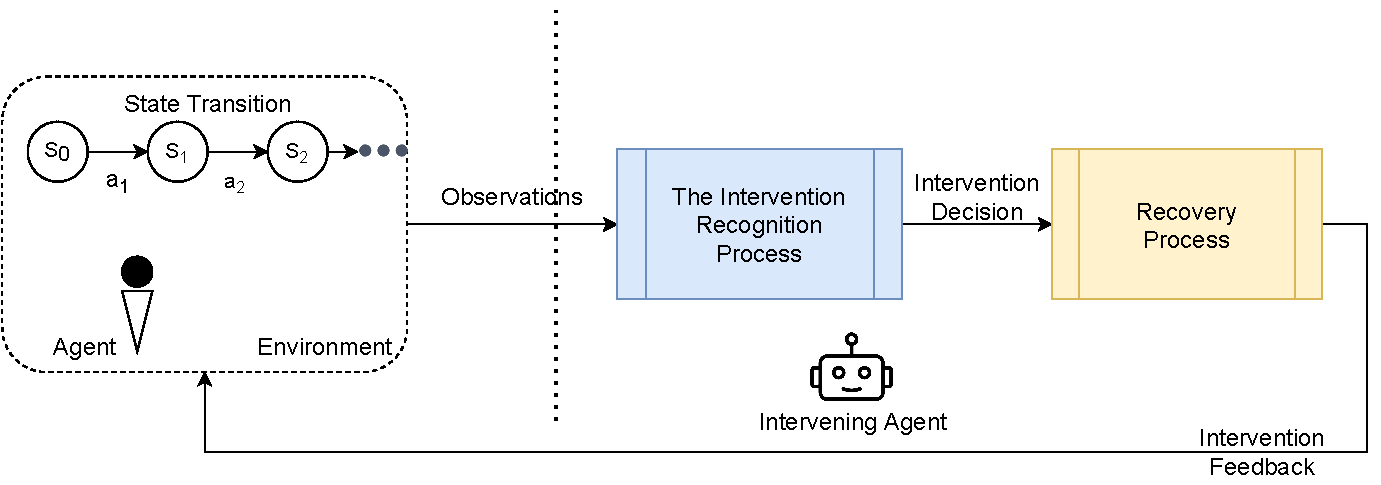
\includegraphics[width=\columnwidth]{img/interventionrecognition.pdf}}
   \caption{The stages of intervention}
\label{fig:stages}
\end{figure}

The second stage of the intervention process is \textit{\textbf{the intervention recovery process}}. 
It is natural to envision the intervention decision to manifest as an alert message for the agent in the intervention feedback loop. 
The simplest case of helping the user through intervention is to adopt a preventive measure such as blocking the recognized dangerous action or displaying an alert.
This approach makes sense in domains like cyber-security because once the attack is complete, reverting back to a safe state may be difficult. 
Furthermore, the user may not even be aware that an attack has taken place until long after. 
Examples of intervention actions include: cleaning attachments of a particular type, updating a software version or installing a firewall. 
In other domains, the preventive measures may not be as helpful. 
For example, if the intervention occurs when the human user is learning to use a new software application, the observer in addition to blocking the action, must also help the user in framing the decision about what to do next.
Therefore, in the intervention recovery process, we ask the question: \textit{can we improve the intervention recovery process to guide the user toward a desirable outcome while avoiding undesirable outcomes instead of blocking actions?} 
This is an important question, specially in cases where the agent is a human user. 
To answer this question, we present an \textbf{intervention feedback technique built on automated planning} to safely guide the user toward the goal.
The intervention feedback technique helps a human user complete a cognitively engaging problem solving task by providing helpful hints. 
A hint is a piece of information about the search problem the user is solving. 
We design helpful hints to allow the user to carefully probe the solution space of the problem during the search, while avoiding the undesirable consequence.
In this dissertation, we explore how automated planning can be used in:
\begin{itemize}
\item modeling the intervention environments
\item intervention recognition process
\item intervention recovery process
\end{itemize}
Automated planning is integral to the design of the intervening agent. 
First, planning is used to model the intervention environment as a state transition system comprised of preconditions and post-conditions of actions. 
Second, to achieve some goal in the environment, the user executes many actions; while a few of them incur risk, some are pivotal in triggering the undesirable consequence. 
Therefore, in order to identify when intervention is needed the observer must be able to generate alternative plans to find the many possible ways to reach the undesirable consequence. 
Third, when intervention occurs the user may still be incapable of deciding what to do next on his own, mainly because of hidden information about the domain or the actions of an adversary that the user can not control. 
Therefore, planning can be used to implement preventive measures such as blocking. 
Once the paths leading to an undesirable consequence have been identified, the planner can be provided with intervention actions that negates the states leading to the undesirable consequence. 
The preconditions of an intervention action are  states that are on the path to the undesirable consequence and the post-conditions of the intervention action negates that specific state. 
In situations where the user needs more help than a simple preventive measure, as we will show in this dissertation, automated planning can be used to help guide the user toward a plan that avoids the undesirable consequence.
Good intervention actions are those that block multiple undesirable consequences, are low cost to execute and do not interfere with the user’s needs or preferences. 
In this dissertation, we discuss three intervention models that address two of the aforementioned requirements, blocking multiple undesirable consequences and not interfering with the user's needs. 
\begin{description}
\item [Recognition of actions that ensures safety while allowing some freedom for the user : ] The observer and the user operate in an unfamiliar and online environment, where partial knowledge about the environment precludes the user from recognizing an unsafe state. 
The observer has knowledge about the user's desirable goal and the unsafe state the user likes to avoid.
We discuss the design of an observer that can intervene and guide a user toward a desirable outcome while avoiding undesirable outcomes or frustration.
When recognizing where intervention is required, the observer considers both the user's goal and the undesirable state.
Furthermore, the observer needs to allow the user reach his goal and not be constantly interrupted.
We present two intervention models that combine automated planning and machine learning. 
The observer can adopt these models to help the user reach the desirable goal while avoiding the undesirable state.
\item [Recognition of actions that enable multiple undesirable consequences : ] Using a cyber-security application, we study intervention when the observer is not aware of the user's goal, but still needs to help the user avoid multiple undesirable states in the environment. 
Because the user's goal is unknown, the observer cannot determine when to intervene based on the user's goal and the undesirable state. Therefore, we frame the observer's decision to recognize when intervention is required as a function of objective metrics. The objective metrics capture the timeliness and criticality of actions that must be flagged for intervention in order to help the observer identify at an opportune time, the actions that may cause the most damage. 
We also investigate how the missing and extraneous actions in the observation trace affects the intervention decision.
\end{description}
In both recognition types, the observer must deal with a trade-off in early recognition of potential danger versus certainty that the undesirable effects will occur. 
In this dissertation, we investigate different metrics to capture that trade-off and how to combine different objective metrics to identify pivotal actions.

\section{The Dimensions of an Intervention Problem}
Let us now look at an example application that requires intervention.
Figure \ref{fig:episode} models an application in the Blocks World domain \cite{gupta1992bw}, where two agents: a user and a competitor stack blocks to spell the words BAND and BRAND respectively.
In the environment, the user and the competitor perform the actions \textsc{pick-up}, \textsc{unstack}, \textsc{stack}, and \textsc{put-down} using the blocks A, B, N, D and R. 
The user can not recognize the block R.
The competitor uses the hidden block R to subvert the user's goal BAND and achieve his goal BRAND.
We refer to the user's goal BAND as the desirable goal (\desired) and the competitor's goal BRAND as the undesirable state (\undesired).
When the competitor and the user present actions to the observer, the observer must help the user achieve BAND while avoiding BRAND. 
The observer does this by accepting actions that help the user advance toward the goal BAND and rejecting the actions that do not. 
In this example, when the user first presents the action \textsc{unstack a b}, the observer asks the question: ``\textit{will the user avoid the undesirable state if the presented action \textsc{unstack a b} is accepted as an observation}?''
If the observer's analysis finds that the user will not avoid the undesirable state, then intervention occurs and the process moves on to the intervention recovery phase.
In the intervention recovery phase, the observer accepts actions that help the user advance toward \desired and rejects actions that enables or satisfies the undesirable state.
The actors continue to present actions until the user achieves \desired.
The observer makes the intervention decisions in favor of the user for each presented action.
\begin{figure}[ptb]
  \centering
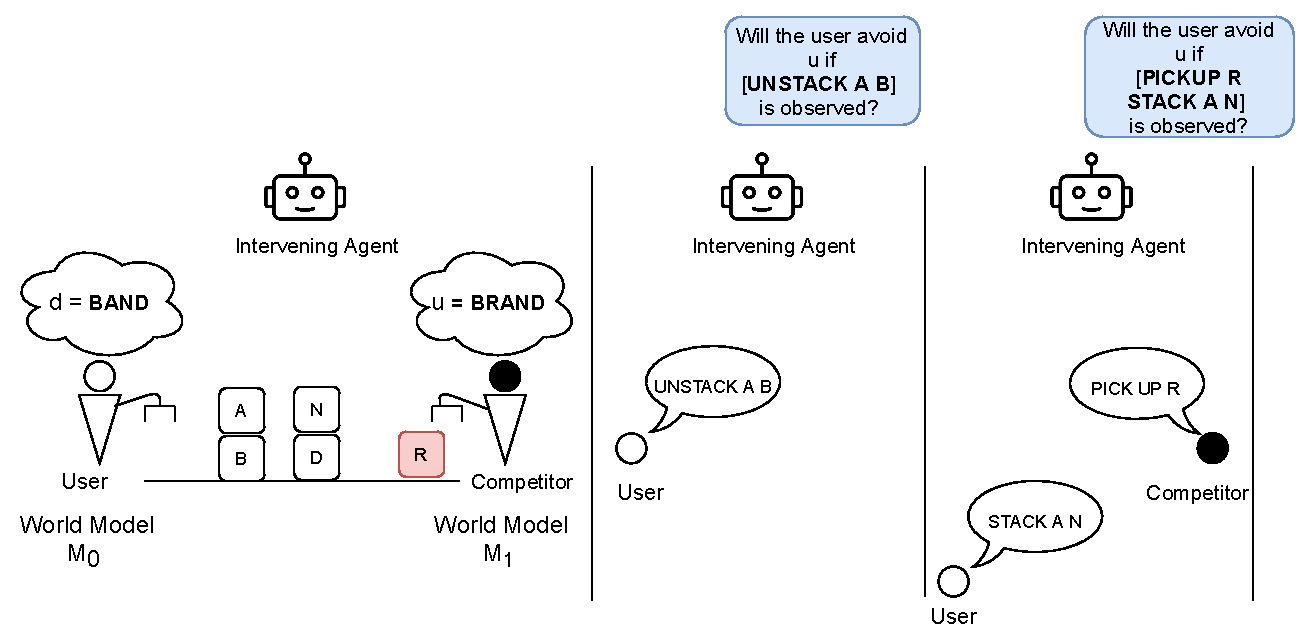
\includegraphics[width=\columnwidth]{img/episode.pdf}
\caption{An intervention episode modeled in the Blocks Words domain}
\label{fig:episode}
\end{figure}

We study several properties in the intervention environment in order to discuss the dimensions of an Intervention Problem, taking a cyber-security application and a cognitively engaging puzzle solving task as examples.
\begin{description}
\item [Actors in the environment :] The observer may be monitoring the user working alone or the user working with other agents in the domain. 
The example in Figure~\ref{fig:episode} shows a scenario where the observer monitors two actors. 
The intervention models we discuss in this dissertation consider both single agent and multi-agent intervention.
When there are other agents working to achieve goals that are different to the user's, the observer must  analyze how the post conditions of the other agents' actions affect the user's goal achievement. 
We can not assume that only the other agent's actions will always result in the undesirable state.
Sometimes, the other agents may execute actions that enable the undesirable state, but the undesirable state does not actually manifest until much later, possibly when the user executes an action that appear to be harmless. 
For example, consider a phishing attack. 
The attacker enables the attack vector by sending the phishing email to steal the user's password. However, the user's password does not get stolen until the user clicks on the link (normally, a  harmless action) to visit the phishing site and submits the information.
Recognizing these enabling actions allows the observer to intervene the user in advance and give the user some time to recover.
\item [Goals hidden to the observer :] To help the user trade-off benefits versus risks, the observer needs to know what the user thinks he/she is trying to accomplish.  
Using automated planning, we can categorize goals of the user and other actors in the environment in terms of  actions and their post conditions. 
However, in certain cases, specifying the user's goal may be difficult. 
For example, consider a home computer user preparing a document to send as an attachment in an email, while listening to music. 
In this situation, the home computer user will not be able to explicitly state his goals as post conditions of actions to the observer as required by planning.
At different times, the human user may change the order in which he wants to achieve the goals. 
For example, at the start he may want to play music in the background (as a secondary goal) while preparing the document (primary goal).
However, if he hears a song he doesn't like he may want to pause the document preparation task and change the song on the music player.
In this situation, the user's priorities change.
Therefore, in certain cases, the observer must also be able to make the intervention decision considering only the undesirable states the user wants to avoid.
\item [Types of observations :] In the example shown in Figure~\ref{fig:stages}, the observer makes the intervention decision based on actions presented by the actors. 
We make the differentiation between observations of actions and observations of state because in some intervention scenarios, the observer may not be able to observe the action itself but will be able to perceive the post conditions of the action in the environment. 
For example, consider the situation where a remote attacker sends a phishing email to the user. The observer may not be able to observe the action of sending the email.
However, the post condition of that remote action, i.e., the presence of the phishing email in the user's inbox, can be perceived by the observer.
When the actions are unobservable, the states resulting from actions can be used to extract the information necessary for the intervention decision.
Our intervention models consider both the observations of actions and states to decide when to intervene.
\item [Noise in observations :] When an agent or a human user executes actions to achieve a goal, lots of extraneous actions can be thrown into the observation trace. 
This is because the user does not intentionally want to trigger the undesirable state. Rather, he is trying accomplish a different (and useful) goal in the domain. 
This means that the plans that lead to the undesirable states may not encompass the user's goal and as a result, the observations will contain not only the undesirable actions, but also the desirable actions.
In addition to extraneous actions, the observer may miss some actions executed by the actors because of faulty sensors. 
Using the cyber-security domain as case study, we explore the impact of noise in the observation trace in making a correct intervention decision.
\item [Intervention recovery :] In this work, we model the observer as an agent who can intervene to help the user reach the desirable goal safely. We present two intervention models with different intervention recovery processes.
In one form of intervention, the observer considers the remaining plans in safe and unsafe partitions to learn to recognize unsafe suffixes in order to help the user avoid the undesirable state.
In this case, the observer can help the user by only accepting actions into the observation history that will safely advance the user toward the user's desirable goal.
In the second form of intervention, the observer learns to recognize that the user is not making progress toward \desired by analyzing the observation history when a suffix is not available. In this case,  the observer must offer enough help to \textit{guide} the user toward \desired without giving the solution. 
The second intervention model is particularly useful when the user is a human and it can be difficult evaluate progress with heuristics like a normal planning agent.
\end{description}


\section{Intervention Use Cases}
Users perform many actions in order to complete a task; while a few of them incur much risk, some are pivotal in triggering vulnerabilities. 
Given there are necessary preconditions in the system, either created by the user or by an adversary, any seemingly harmless action can suddenly become dangerous. 
The Intervention models allow us to automatically detect such vulnerable situations.
We discuss helpful intervention using two use cases. 
The uses cases we selected to study intervention have different dimensions. 
Table \ref{tab:properties} summarizes the intervention dimensions for each domain.
\begin{table}[tpb]
\caption{Dimensions of intervention use cases}
\label{tab:properties}
\resizebox{\columnwidth}{!}{%
  \begin{tabular}{|l|l|l|}
\hline
& \multicolumn{2}{c|}{\textbf{Domain}}  \\ \cline{2-3} 
\multicolumn{1}{|c|}{\textbf{Dimension}} &
  \multicolumn{1}{c|}{Cyber-security} &
  \multicolumn{1}{c|}{Rush Hour} \\ \hline
Actors in the environment  & User, Attacker, Observer & User, Observer \\ \hline
Goals hidden to the observer &
  \begin{tabular}[c]{@{}l@{}}User's goal is hidden\\ 
  Multiple known undesirable states \end{tabular} &
   \begin{tabular}[c]{@{}l@{}}User's goal is not hidden\\ 
  One or more known undesirable states \end{tabular} \\ \hline
Types of observations &
  \begin{tabular}[c]{@{}l@{}}The observer observes user's actions\\ 
  The observer only observes the effects of the attacker's actions\end{tabular} &
  The observer observes user's actions \\ \hline
Noise in observations     & Has missing and extraneous observations & None                           \\ \hline
Intervention recovery  & block action & Offer helpful hint   \\ \hline
\end{tabular}%
}
\end{table}

\subsection{Intervention in Cyber-security}
In the cyber-security domain, we model an attacker attempting to trick the user into compromising his security/privacy during day-to-day computing tasks.
The attacker creates opportunities for phishing and malware attacks by making them to appear as common harmless tasks such as email and installing software.
Unable to recognize these attacks in advance, the user becomes an unwitting accomplice to security breaches. 
The Intervention Problem for the cyber-security domain consists of three actors: the human user, the attacker (human/machine) and the observer. 
In most cyber-security cases, the attacker does not operate as a typical adversary (e.g., taking turns with the user). 
Instead the attacker takes preemptive actions and lays traps (e.g., send phishing email), which are often tied to typical actions the user performs (e.g., checking email). 
We model the cyber-security domain with multiple undesirable states: phishing attacks, malware installations. However, the user's goal is hidden to the observer.
In the cyber-security domain we model noisy observations in terms of missing and extraneous actions.
The observer considers the actions of the user and the post-conditions of attacker's actions to produce the intervention decision. 
The observation trace will contain varying noise levels from missing and extraneous actions.
Our helpful intervention solution for cyber-security is based on automated planning and uses the properties of a planning problem to identify ``\textit{critical trigger actions}'', that will cause the security breach. 
We do not study a specific recovery process for Cyber-security domain. 
We assume that when the observer identifies the critical trigger action, it is blocked.

\subsection{Intervention in Rush Hour}
Our second case study is a puzzle solving task called Rush Hour, which simulates a parking lot. In the standard version of the puzzle, the player has to clear a path on a board to move a target vehicle to the exit. To simulate the condition where the user is working only with partial knowledge about the domain, we introduced a hidden forbidden vehicle to the Rush Hour puzzle, which if moved will cause the undesirable state. 
We use the Rush Hour puzzle to approximate the case where human users learn to use a new software application and also it helps motivate the users to actually do the task in experiment conditions. 
The Rush Hour domain only has the human user and the observer. 
Unlike the cyber-security use case, the observer is aware of the desirable goal the user is trying to achieve (i.e., solve the puzzle by moving the target vehicle to the exit) and also the undesirable state (i.e., forbidden vehicle moves).
Similar to the cyber-security use case, the Rush Hour domain also contains multiple undesirable states. All states resulting from legal moves of the forbidden vehicle are undesirable.
The observations are actions the user executes to solve the puzzle. In this case, the observations are not noisy.
Our intervention solution for this case uses machine learning algorithms to recognize when the user is about to move the forbidden vehicle and intervene.
As the recovery process, we explore how to help the human user decide what to do next by offering further assistance as helpful hints.
In both cases the user actively pursues his own goal. 
The threats are triggered because the user did not understand the consequences of reaching the undesirable state (phishing/malware vulnerabilities) or was not aware of the undesirable state from the start (hidden forbidden vehicle in Rush Hour). 
The observer makes the decision to intervene upon recognizing actions in the observations that enable or satisfy the undesirable state.
 
\section{Distinguishing Intervention From Plan Recognition}
Plan recognition is the closest to our Intervention Problem. 
In the literature the plan recognition is defined as the problem of taking as input a sequence of actions performed by an actor and inferring the goal pursued by the actor and also organizing the sequence as a plan structure \cite{kautz1986generalized,schmidt1978}. 
The solution to the plan recognition problem is given by the set of goals that produces a plan that is compatible with the observations. 
The online version of the plan recognition problem uses observations as they happen as input. 
The offline version requires the complete observation to be available in advance. 
At first glance, it might seem that intervention is a variant of Plan Recognition for the user's desirable goal and the undesirable states the user wants to avoid. 
However, there are several subtleties that make intervention unique, which we now discuss.
\begin{itemize}
\item \textbf{Intervention is an online problem.}
In most cases Plan Recognition (e.g., \cite{ramirez2009plan,ramirez2010probabilistic, sohrabi2016plan}) is an offline problem;
there are a few notable exceptions \cite{mirsky2018}.
However, intervention is inherently online and dynamic.  
The observer decides whether to intervene (or not) every time the user(s) presents an action.
In order to make the decision, the observer uses the observation history, which contains accepted actions.
Intervention is a multi-agent problem as well. 
This has ramifications in environments where the user and the competitor compete to achieve close but different goals. 
With intervention, the observer can help the user by accepting actions into the observation history that only help further the user's goal. 
This is not possible with offline plan recognition.
\item \textbf{Agents may have distinct views of the problem.}  
The user and the competitor are modeled with different domain definitions. 
When the agents have distinct views of the problem and they can not satisfy the undesirable state on their own, conditions will arise such that the agents working together will enable the undesirable state.
The user wants to satisfy the desirable goal state, while avoiding the \textit{hidden} undesirable state.
The competitor is trying to subvert the user’s goal by enabling preconditions for the undesirable state without the user's knowledge.
When the user and the competitor reveal their plan(s) incrementally, the observer needs to decide whether the revealed actions make it impossible for the user to avoid the undesirable state considering the plans from the user's and the competitor's domain definitions collectively. 
Any action that make it impossible for the user to avoid the undesirable state must be flagged for intervention and not accepted into the observation history.
If the plans for the undesirable state and desirable goal share a long common prefix, 
it will be difficult for the observer to disambiguate between the goals and to use plan recognition algorithms in time to help the user avoid the undesirable state.
\item \textbf{Partitioned suffixes (with known desirable goal).}
When the desirable goal is known, the observer should allow the user to pursue suffixes leading to the desirable goal and intervene when actions are presented from suffixes that get ``too close'' to the undesirable state. 
Our key insight is to model the  ``goals'' of the user and competitor, which justifies our use of planning to find these suffixes. 
However, intervention adds new concerns beyond plan recognition, namely that the observer needs to consider two kinds of goals that might require intervention:
\begin{enumerate}
\item Cases where the user is headed toward a undesirable outcome. 
This can be easily be solved by plan recognition.
\item Cases where the user unwittingly enables an undesirable outcome by taking actions toward a desired goal. 
This is less easily solved by plan recognition because there is an inherent trade-off between intervening and allowing the user some freedom to pursue the desirable goal. 
Suppose that some suffix $\Suffix_{\undesired}$ leads to the undesirable state and suffix $\Suffix_{\desired}$ leads to the desirable goal.  
Then it can happen that by simply following the plan leading to the desirable goal, the user enables the undesirable state when there is enough overlap between  $\Suffix_{\undesired}$ and $\Suffix_{\desired}$.
\end{enumerate}
Partitioning the suffixes this way allows the observer to learn the differences between the safe and the unsafe suffixes and balance specific unsafe actions with those that are necessary for allowing the user some freedom.
For example, in a malicious email attack such as phishing, the user will still want to check email.
So prohibiting email is untenable; what the agent must do is intervene when the user attempts to click the phishing link.
This need for partitioning the suffixes  is distinct from plan recognition, where existing offline Plan Recognition algorithms often rely on  plan cost to disambiguate between goals and recognize suffixes. 
When the undesirable state and the desirable goal are too close, disambiguation based on plan cost will not work (we will demonstrate in a later chapter). 
Learning the differences between the plan partitions will allow us to address this issue.
\item \textbf{Suffix analysis with unknown desirable goal.}
When the desirable goal is unknown, the observer only has the space of plans leading to the undesirable goals to make the intervention decision when the agents reveal their plans incrementally.
Plan recognition over the undesirable goals does not really     apply because it is     focused on matching actions to  prior plans     to determine the goals the      user is trying  to achieve.     
In other words, the observer assumes that the user is executing some plan to reach the undesirable state.
In reality, the user wants to avoid the undesirable state and reach a different (desirable) goal, which may be unknown to the observer.
Therefore, when analyzing partition suffixes with known desirable goal, the observer uses the knowledge of the user's goal to determine which are critical actions that require intervention.   
In contrast, with unknown desirable goal, the observer analyzes the remaining undesirable suffixes to identify actions that cause the most damage to intervene the user.
\item \textbf{Goal priors cannot be estimated reliably.}  
Plan Recognition algorithms use a prior probability distribution over the goal hypotheses to estimate the posterior probability of the likely goals given the observations. 
Intervention must consider the likely goals regardless of their priors. 
For example, the undesirable state is hidden from the user, who does not intend to achieve it (i.e., prior probability $\approx 0$). 
In contrast, a competitor, when present, intends to achieve the undesirable state (i.e., prior probability $\approx 1$).
When the priors are not accurate, the observer (using Plan Recognition) may not be able to  disambiguate between likely goals (and recognize the correct plan) in time to avoid the undesirable state.
  
\item \textbf{Emphasis on intervention recovery.}
In Plan Recognition, the observer uses an observation trace to derive the user's likely plan. 
The observation trace can be either an ordered sequence of actions  \cite{ramirez2009plan,ramirez2010probabilistic} or an ordered sequence of states \cite{sohrabi2016plan}.
Plan Recognition does not define a method for the user to recover when the observer recognizes a plan leading to the undesirable state. 
With the proposed intervention models, we address that limitation with two different types of help the observer can offer to the user to decide what to do next.
\end{itemize}


\section{Research Questions}
The main objective of this research is to study different intervention models that help human users complete tasks safely. We address the following research questions: 
\begin{description}
\item[What are the salient characteristics for deciding when to intervene?]
We address this question considering the dimensions of an intervention problem, summarized in Table~\ref{tab:properties}.

Our intervention models are based on identifying actions in an observation trace that either satisfy the undesirable state or enable it. 
This requires the observer to evaluate the current state (i.e., state resulting from the observed actions) based on it's importance to causing the undesirable state considering the user's desirable goal (if available) and the undesirable state.
In the two intervention use cases, criticality of the current state is evaluated using two different methods. 
For the cyber-security domain we identify salient features by analyzing the plan space. 
We model the cyber-security domain as a planning problem and use an existing automated planner to  sample the possible solutions (plans) that project possible undesirable outcomes and then trace back to actions critical to their occurrence. 
The resulting plans are analyzed to extract objective metrics to predict if the current action is likely to trigger the undesirable consequences. 
Raising a warning to the user involves a trade-off in early recognition of potential danger versus certainty that the effects will occur. 
We investigate different objective metrics to capture that trade-off and how to combine these objective metrics to identify pivotal actions. 

To study intervention in the Rush Hour domain, we formalize a family of Intervention Problems and show how these problems can be solved using a combination of Plan Recognition methods and classification techniques to decide whether to intervene. 
We characterize the observer's decision space as an Intervention Graph and construct it using an ``Intervention as Classical Planning'' approach to generate potential suffixes of partially executed plans. 
We extract domain-independent features from this graph and extend several Plan Recognition benchmarks to evaluate this approach. 
We then generalize these results to Human-Aware Intervention, where the observer must decide in
real time whether to intervene for human users solving a cognitively engaging puzzle. 
Using a revised feature set more appropriate to human behavior, we produce a learned model to recognize when a human user is about to trigger an undesirable outcome.

\item[How should information be displayed to effectively inform users following intervention?] Using the Rush Hour domain, we study how an intervention model can be extended to help users continue a cognitively engaging task by providing helpful hints. 
In the context of the Rush Hour puzzle solving task, a hint is a piece of information about the Rush Hour search problem. 
We design helpful hints to allow the user to carefully probe the search space of the Rush Hour search problem, while avoiding the undesirable state.
We monitor how human users achieve planning landmarks of the Rush Hour problem when intervention is supported by hints compared to intervention without hints to evaluate the effectiveness of our intervention recovery process.

\item[How to design tools to study intervention in activities with human user participation?]
To identify pivotal events, the appropriate system states and user actions must be monitored and compared to a model of actions that can lead to the undesirable state. 
If an action that contributes to a trigger is suspected, it should be put in the context of what the user is trying to do and an estimate of how likely the action is to actually cause the undesirable state. 
We develop state/action models using automated planning that allow us to recognize the appropriate system \textit{states} (computer/puzzle board) that must be monitored and the \textit{actions}, which may lead to the undesirable state. 
For the cyber-security domain, we model the security vulnerabilities that occur in a home computer environment using PDDL (Planning Domain Definition Language) \cite{ghallab1998}, which is designed to represent pre-conditions and post-conditions of actions. 
PDDL is the prominent representation used in the AI Planning community. 
We also develop PDDL models for the Rush Hour domain, which will be used in generating the helpful hints. 
Our studies are focused on how human users solve these tasks (e.g., perform common home computer user actions, solve a Rush Hour puzzle), which requires studying human users in situ. 
To this end, we will develop a simulated home computer environment for studying users practice computer security and a Rush Hour puzzle simulator to study how human users respond to helpful hints. 
Both these tools are event monitoring systems that capture human user's actions when placed in different experimental conditions as well as system level events that are defined in the PDDL models.
\end{description}


The rest of this dissertation is organized as follows:
\begin{itemize}
\item \textbf{Chapter 2}: We present the background on automated planning and a review of existing plan recognition literature that studied methods to infer an agent's intention.
\item \textbf{Chapter 3}: We present the findings of an human subject study to motivate plan intervention. In this study, we simulate cyber-security vulnerabilities that occur in a home computer environment when the human users perform routine tasks like checking email and using software applications.
\item \textbf{Chapter 4}: We present the first intervention model based on the findings of the cyber-security human subject study. 
We formulate the Intervention Problem as a  planning problem of three domain independent objective metrics: timeliness, which captures how soon the undesirable state may occur; certainty, which captures how frequently the undesirable state may be seen; and desirability, which captures the user’s preference for continuing the current action despite the increased risk. 
Against an ideal baseline, we examine trade-offs in choosing the ``correct'' intervention point by varying the weights associated with these objective metrics, the observability of actions, and the presence of extraneous actions.
\item \textbf{Chapter 5}: We study two kinds of Intervention Problems in environments where an observer monitors a user (and a competitor) and help the user achieve a desirable goal, while avoiding an undesirable state. 
In ``\textbf{Unsafe Suffix Intervention}'', the observer uses automated planners to project the remaining suffixes and extract features that can differentiate between safe and unsafe plans. 
We evaluate the recognition accuracy of Unsafe Suffix Intervention on benchmark planning
problems. 
In ``\textbf{Human-aware Intervention}'', the observer uses the observed partial solution to extract features that can separate safe and unsafe solutions. 
We evaluate the accuracy of Human-aware Intervention on a new Intervention Planning benchmark Rush Hour.
\item \textbf{Chapter 6}: We present an intervention recovery process for the Human-aware Intervention model based on automated planning. 
We discuss the findings of a human subject study where human users solved a cognitively engaging Rush Hour puzzle task while being guided by a human-aware intervention agent. 
We evaluate the efficacy of our recovery approach using automated planning landmarks.
\item \textbf{Chapter 7}: We discuss some open issues in Intervention and provide an outline for future research.
\end{itemize}


\chapter{Preliminaries}
\label{chap:ch2}
In order to design intervention for human users, first we need to model human user behavior in some environment. 
We use the automated planning formalism \cite{nau2004} to describe the tasks the user performs in both the cyber-security and Rush Hour domains. 
The automated planning formalism is based on concepts such as goals, states and actions, to describe the behavior of rational agents. 
Although human user behavior is more complex than that of a rational agent, in our intervention models we assume the actor being intervened is a (bounded) rational agent.
In this chapter, we first present an overview of automated planning and describe how a state/action model can be represented as a classical planning problem. Next, we discuss the problem of inferring the intention of an agent and discuss three variants of the problem: plan recognition, goal recognition and activity recognition. Finally, we present a discussion on the existing literature on intention recognition considering a three-dimensional framework: number of agents in the environment, online/offline recognition and how the recognizer interacts with the environment during the intention recognition process.

\section{Automated Planning}
Planning aims at achieving some predefined objectives through a deliberation process that chooses and organizes actions by anticipating their outcomes. The planning formalism views the problem as a state transition system, defined as a tuple $\Sigma=(S,A,E,\gamma)$ where:
\begin{itemize}
\item $S = \lbrace s_1, s_2, \ldots \rbrace$ is a finite or recursively enumerable set of states;
\item $A = \lbrace a_1, a_2, \ldots \rbrace$ is a finite or recursively enumerable set of actions;
\item $E = \lbrace e_1, e_2, \ldots \rbrace$ is a finite or recursively enumerable set of events; and
\item $\gamma: S\times(A\cup E)\mapsto 2^S$ is a state transition function.
\end{itemize}
Given an action $a\in A$ and $\gamma(s,a)\neq\emptyset$, then $a$ is \textit{applicable} in state $s$. If $a$ is applied to the state $s$, it will take the system to a different state $s^\prime\in \gamma(s,a)$. A state transition system $\Sigma$ can be represented in a directed graph $G=(V_G,E_G)$, where $V_G=S$ and an edge $e_G\in E_G$ connects two states $e_G=s\mapsto s^\prime$, labeled with an action $a$ if and only if $s^\prime \in \gamma(s,a)$ as shown in Figure~\ref{fig:blockswords}. 

In this example, we model the Blocks Words problem \cite{ramirez2009plan}, which is a modification of the Blocks World domain \cite{gupta1992bw}. In the Blocks Words problem, the agent operates in an environment that contains a flat surface (a table) and a set of blocks identified by English letters. The blocks can be stacked on one another. The agent uses a set of actions (e.g., pick-up, put-down, stack, unstack) to build a stack such that it spells a word from the top to bottom (i.e., goal state). The agent can only move one block at a time. The agent's goal is to spell the word BAND. Initially, the blocks D, N are on the table and B is stacked on A. The partial graph shows some of the the state transitions that can happen in the domain. Red color edges show a path (i.e., an action sequence), which translates the initial state to the goal state. Let us map the Blocks Words environment in Figure \ref{fig:blockswords} to the definition of $\Sigma$.
\begin{itemize}
\item $S = \lbrace init, goal, s_1, s_2 \ldots \rbrace$ is a finite or recursively enumerable set of states;
\item $A = \lbrace pickup, unstack, stack, putdown \rbrace$ is a finite or recursively enumerable set of actions;
\item $E = \lbrace \rbrace$ assuming no exogenous events occur and;
\item $\gamma:$ transitions indicated by arrows in the graph.
\end{itemize} 


The state transition system $\Sigma$ describes all the ways in which our environment may evolve. Finding a \textit{plan} means that we need to extract a structure that gives appropriate actions to apply such that some \textit{objective} can be achieved. There can be many forms to define this objective: (1) defining a goal state or a set of goal states (e.g., state \textit{Goal} in Figure~\ref{fig:blockswords}), (2) optimize for a utility function attached to the states, (3) satisfying some condition over the sequence of states, (4) defining tasks to be performed. In our work, when we refer to the \textit{objective}, we mean type (1) objective.

The preliminary intervention designs are for an agent whose behavior can be represented using a classical planning model. The classical planning formalism requires eight restrictive assumptions about $\Sigma$:
\begin{enumerate}
\item The system is defined using a \textbf{finite} sets of states, actions and events.
\item The system defined in $\Sigma$ is \textbf{fully observable}. This means that the agent has knowledge  about every aspect of the state when an observation is made.
\item The system defined in $\Sigma$ is \textbf{deterministic}, i.e., an action in the system does not have alternative outcomes. Formally, for all $s\in S, u\in A\cup E; |\gamma(s,u)|\leq1$
\item The system define in $\Sigma$ is \textbf{static}, i.e., there are no exogenous events happening in the environment. $E=\emptyset$
\item Only \textbf{restricted goals} can be given to the planner. Restricted goals are given as an explicit goal state or a set of goal states.
\item The solution plan for a planning problem in $\Sigma$ is a linearly ordered finite sequence of actions.
\item The system defined in $\Sigma$ has \textbf{implicit time}. This means that actions and events do not have any time duration between state transitions.
\item Planning in $\Sigma$ is \textbf{offline}, which means that any changes to $\Sigma$ that takes place while the planner is searching for a plan, are ignored.
\end{enumerate}

Given a description of $\Sigma$, the initial state and an objective, an automated planner generates a plan that achieves the objective. A classical plan for the Blocks Words problem is a sequence of actions (e.g., \texttt{unstack B A, put down B, pick up N}, etc.). A plan can also be represented as a policy: a partial function from $S$ into $A$ (e.g.,  $\lbrace$(\texttt{init, unstack B}), ($s_1$,\texttt{ putdown B}), ($s_4$,\texttt{ pickup N}) $\ldots\rbrace$. When we refer to plans in this work, we mean a sequence of actions. The agent can execute these plans on the environment using actuators, which generates observations. In our Blocks Words example, the agent can use a mechanical arm to lift block B from the top of A. This generates an observation, the mechanical arm holding block B and the top of block A now being clear. Formally, the agent's behavior can be defined as a \textbf{planning problem} $P=(\Sigma, s_0, S_g)$ where, 
\begin{itemize}
\item $\Sigma=(S,A,\gamma)$ is a state transition system,
\item $s_0\in S$ is the initial state and
\item $S_g\subset S$ is a set of goal states.
\end{itemize}
\noindent The solution to $P$ is a sequence of actions $\langle a_1, a_2, a_3, \ldots, a_n\rangle$ such that it corresponds to a sequence of states $\langle s_0, s_1, s_2, \ldots, s_n\rangle$ where $s_1=\gamma(s_0,a_1), s_2=\gamma(s_1,a_2), \ldots, s_n=\gamma(s_{n-1},a_n)$ and $s_n \in S_g$

\begin{figure}[ht]
  \centering
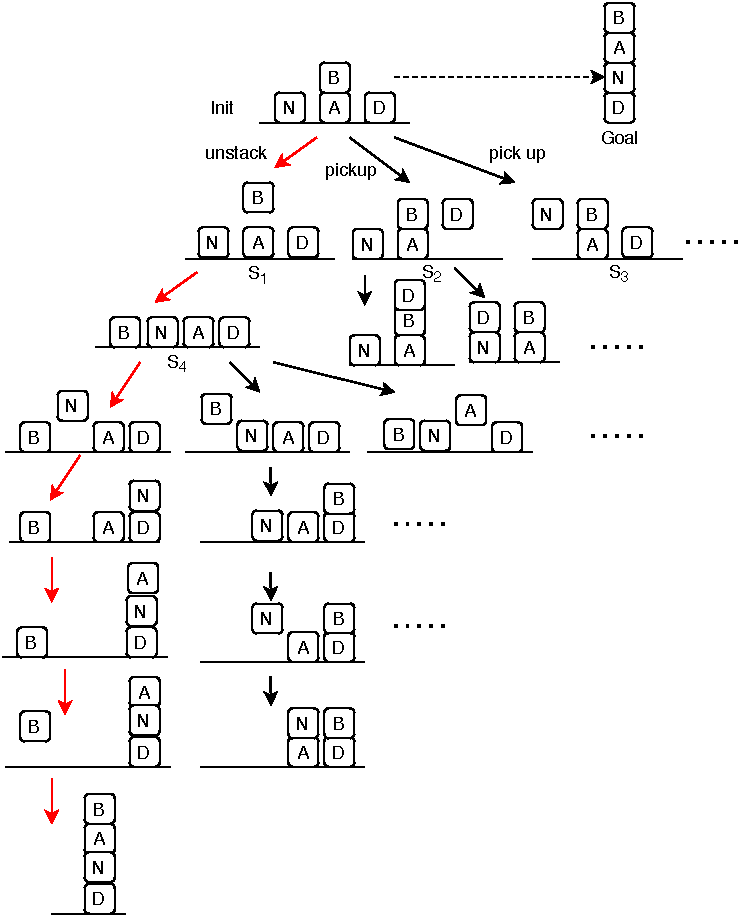
\includegraphics[width=0.6\columnwidth]{img/bw.pdf}
  \caption{Blocks Words problem as a state transition system}
  \label{fig:blockswords}
\end{figure} 

\section{Representing Classical Planning Tasks}
Although we can use the graph representation of the state transition system corresponding to a planning problem, the resulting graph can be very large and modifying this graph as new events occur in the system can become very cumbersome. In order to provide a compact representation of the transition system, \textit{states} (i.e., vertices) are represented using state variables, and actions (i.e., edges) are represented as \textit{operators} with preconditions and post-conditions specified as state variables. This way, in order to find a plan, we only need to provide the initial and goal states and use the operators to find other states as needed.

A classical planning problem can be represented using the \textbf{classical representation}, \textbf{the set-theoretic representation} or \textbf{the state-variable representation}. STRIPS \cite{fikes1971strips}, which we will use to model the domains described in this work, is an implementation of the classical representation. STRIPS uses first-order literals to describe states and actions. The set-theoretic representation is used when planning problems are solved with SAT solvers. The state-variable representation is implemented in SAS formalism \cite{backstrom91}.

In the classical representation, the world state is a set of \textbf{grounded} propositional state variables. $\Sigma$ is described using a finite set of grounded propositional state variables, which means there are only finitely many possible states. Operators that modify the world state consist of precondition propositions: propositions that must be true for the action to execute, and post-condition propositions: those will be made true as a result of the action. An \textit{action} is a ground instance of an operator. The initial state in the Blocks Words example in Figure~\ref{fig:blockswords} described in the grounded classical representation is: $\lbrace$
\texttt{ontable(N)}, \texttt{ontable(A)}, \texttt{ontable(D)}, \texttt{on(B,A)}, \texttt{clear(N)}, \texttt{clear(B)}, \texttt{clear(D)}$\rbrace$. The operator unstack is described as: \\
\textbf{operator}: \texttt{unstack (x, y)}\\[-0.5em]
\textbf{preconditions}: \texttt{(on x, y)},\texttt{(clear x)},\texttt{(handempty)},$\neg$\texttt{(equals x y)}\\[-0.5em]
\textbf{effects}: \texttt{(holding x)},\texttt{(clear y)},$\neg$\texttt{(clear x)},$\neg$\texttt{(handempty)},$\neg$\texttt{(on x, y)}

\noindent Grounding the unstack operator using blocks B and A defines the action as follows:\\
\textbf{action}: \texttt{unstack (B, A)}\\[-0.5em]
\textbf{preconditions}: \texttt{(on B, A)},\texttt{(clear B)},\texttt{(handempty)},$\neg$\texttt{(equals B A)}\\[-0.5em]
\textbf{effects}: \texttt{(holding B)},\texttt{(clear A)},$\neg$\texttt{(clear B)},$\neg$\texttt{(handempty)},$\neg$\texttt{(on B, A)}

\noindent An action is \textit{applicable} in state $s$ if $s$ satisfies the preconditions of the action. 
This means that the action's positive preconditions are  in $s$ whereas the negative preconditions are not in $s$. 
In the Blocks World example, (\texttt{unstack B A}), (\texttt{pickup D}), and (\texttt{pickup N}) are applicable in the initial state. If an action is applicable to $s$, the result of performing the action means to delete the negative propositions from the state $s$ and add the positive ones. For example, if \texttt{unstack B A} is executed in the initial state, the resulting state would be $\lbrace$ \texttt{ontable(N)}, \texttt{ontable(A)}, \texttt{ontable(D)}, $\neg$\texttt{on(B,A)}, \texttt{clear(N)}, $\neg$\texttt{clear(B)}, \texttt{clear(D)}, $\neg$(\texttt{handempty}), \texttt{clear (A)}, \texttt{holding (B)}$\rbrace$. Typically, in the classical representation, the state only explicitly contains the true propositional variables. Any propositional variable that are not included in the state is considered false.


\subsection{STRIPS Planning Task}
We now present a formal definition of a STRIPS domain and planning problem. In STRIPS, a planning task is defined using a planning domain and a planning problem.
\begin{definition}
A STRIPS planning domain is a tuple $\mathcal{D}=\langle F, Op\rangle$, where $F$ is a finite set of  state variables (predicates) and $Op$ is the set of operator schema. An operator schema $op \in Op$ is a tuple $ op = \langle Pre(op), Add(op), Del(op)\rangle$ that consists of preconditions, add and delete effects respectively, where $Pre(op)$, $Add(op)$, $Del(op)$ are all subsets of $F$. Predicates and operator schema have parameter lists and can be instantiated with objects (defined later). An instantiated operator (action) $op$ is applicable in a state $s$ if predicates in $Pre(op)$ are \textit{True} in $s$. A state transition induced by an action $op$ in a state $s$ is defined as a function $\delta$:
\begin{equation*}
\delta (s,op) = \left\{\begin{matrix}
s\setminus Del(op) \cup Add(op) & Pre(op) \subseteq s\\ 
undefined & otherwise
\end{matrix}\right.
\end{equation*}
\end{definition}

\begin{definition}
A STRIPS planning problem is a tuple $P = \langle \mathcal{O}, s_0, G\rangle$, where $\mathcal{O}$ is the set of objects. Objects can be either constant or non-constant and may have a type. Constant objects are common to all instances of the domain definition and shared by planning problems defined on that specific planning domain. Non-constant objects are unique to a specific planning problem. $s_0 \subseteq F$ is the set of propositions that are true in the initial state, $G\subseteq F$ represents the goal specification.
\end{definition}

Given a domain $\mathcal{D}$ and a planning problem $P$, an automated planner generates the planning task $\Pi=\langle \mathcal{F}, \mathcal{A}, s_0, G\rangle$, where $\mathcal{F}$ is a finite set of grounded propositions, $\mathcal{A}$ is the finite set of grounded actions instantiated from the operator schemata $Op$, $s_0$ is the grounded propositions specifying the initial state and $G$ is the grounded goal specification. Objects in $\mathcal{O}$ are used to ground $\mathcal{F}$, $\mathcal{A}$, $s_0$ and $G$. Grounding replaces the variable terms in the parameter lists of the propositions, action schema, goal specifications with constant/non-constant objects. 

\begin{definition}
A solution to $\Pi$ is a plan $\pi=\lbrace a_1, \ldots, a_k\rbrace$ of length $k$ that modifies $s_0$ into $G$ by successive execution of actions  $a_1, \ldots, a_k$ 
\end{definition}

Actions in $\pi$ may have a cost that assigns a non-negative value to the action schema defined in the STRIPS domain definition. The cost function is given as $C: Op \rightarrow \mathbb{R}^0_+$. The cost of the plan $c(\pi)$ is  $\sum(c(a_i))$. The optimal solution, the optimal plan $\pi^*$, minimizes the cost. 



\section{The Recognition Task}
Besides being able to plan, in certain cases the agent must also be able to \textit{recognize} another agent's behavior. This is specially important in the domains we are studying in this dissertation where the agent acts as an assistant to the human user.

We now extend our discussion to a multi-agent setting where, we consider at least two agents: an  acting agent $A$ and an observer agent $R$. To draw a realistic example, consider the Blocks World scenario in Figure~\ref{fig:bwpr}. Agent $A$ solves a planning task $\Pi_A=\langle \mathcal{F}_A, \mathcal{A}_A, s_{I_A}, G_A\rangle$ executes a sequence of actions $O=\lbrace$\texttt{unstack D A}, \texttt{putdown D}, \texttt{unstack R P}$\rbrace$. For simplicity let us assume that $R$ does not execute any actions, and passively observes the actions $A$ executes.

\begin{figure}[tpb]
  \centering
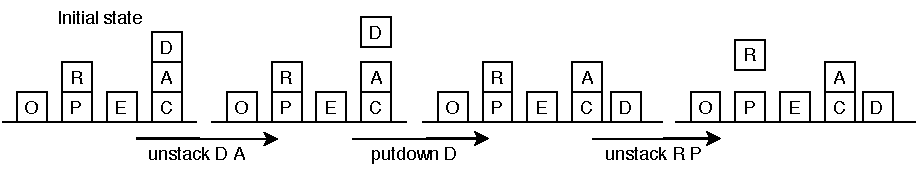
\includegraphics[width=\columnwidth]{img/bwpr.pdf}
  \caption{A recognition task}
  \label{fig:bwpr}
\end{figure}

\noindent In the recognition task, $R$ asks the question: ``What is $A$ trying to do?''. This question can be answered in three ways, leading to three types of recognition tasks:
\begin{itemize}
\item Given $O$, what is the posterior probability P($\pi$|$O$) of the complete plan $\pi$. This is the \textbf{plan recognition problem}.
\item Given $O$, what is the posterior probability P($G$|$O$) of the goal $G$, where $G \in \mathcal{G}$, a list of potential goals in the environment. This is the \textbf{goal recognition problem}
\item Given $O$, what is the posterior probability P($a$|$O$) of an activity $a$. This is the \textbf{activity recognition problem}.
\end{itemize}
\noindent Typically, $R$'s objective is to find the most likely plan, goal, activity from a set of potential plans, goals, activities in the environment. A recognition task consists of three components:
\begin{description}
\item [The environment] $E = \lbrace \Sigma, s_0, \mathcal{G}\rbrace$, is the setting in which agent $A$ acts. $s_0$ is the initial state and $\mathcal{G}$ is the set of possible goals. 
In order to perform the recognition task, the environment may produce a \textbf{plan} $\pi=\lbrace a_0, a_1, \ldots, a_n\rbrace$: a complete sequence of actions that takes agent $A$ from $s_0$ to the goal state $G$ in $\mathcal{G}$, a \textbf{history} $h=\lbrace s_0, s_1, \ldots, s_n\rbrace$: a sequence of states from $s_0$ to $G$ or an \textbf{execution} $e=\lbrace s_0, a_0, s_1, a_1, \ldots, s_n, a_n, s_{n+1}\rbrace$: a sequence of state-action transitions from $s_0$ to $G$. 
These are referred to as \textit{prefixes} in recognition. 
The recognition task example shown in Figure~\ref{fig:bwpr} considers the plan prefix. Some work in the plan recognition literature uses plan prefixes while others use the history prefixes. We will discuss work on each category. Furthermore, research has investigated recognition in both discrete and continuous domains where actions transition from one state to another via paths through the state space, rather than through discrete states (e.g., navigation domains).

\item [The acting agent (agent $A$)] must specify the assumptions made with regard to how agent $A$ acts in the environment to achieve his goal. Most of the time, recognition tasks assume that agent $A$ enters the environment and follows a plan to achieve some goal. However, $A$'s behavior may be affected by how familiar it is with the environment (e.g., are there objects that escape agent $A$'s sensors?), A's special capabilities (e.g., can he compute an optimal plan to reach $G$), and the relationship to the recognizer (e.g., does $A$ acts in such a way that his goal/plan/activity can be recognized easily or would he act to obfuscate his true goal/plan/activity?). There could be more than one agent whose goals/plans/activities we would want to recognize.
The recognition literature uses different ways to represent agent $A$ from the point of view of $R$ in the situations mentioned above. Commonly used representations are \textbf{plan libraries} and \textbf{domain theories}.

\item [The recognition system (agent $R$)] When defining a recognition problem, the final component is the specification of the recognizer. Here, we need to define several components: 
\begin{itemize}
\item the observability: how does agent $R$, perceive agent $A$'s behavior (e.g., is there any noise in the observations? Are there any actions/states $R$ can not perceive?)
\item the objective: what does $R$ need to do? (e.g., recognize $A$'s goal/plan/activity as soon as possible? is the recognition online or offline?)
\item the possible interventions: can $R$ interact with $A$ or affect its behavior? (e.g., provoke $A$ to change its course during execution, modify $\Sigma$ to help recognition)
\end{itemize}

\end{description}

We now present a framework, within which we discuss selected prior work from goal and plan recognition. We set up the framework along three dimensions:
\begin{description}
\item [single vs. multi actor] In the single actor case, $R$ makes observations of a single actor agent to recognize the goal/plan of that agent. In the multi-agent case, the observations originate from many agents. Furthermore, the goals pursued by the agents in the system may be a complex goal. For example consider an agent $X$ assisting two other agents ($Y$ and $Z$) pursuing two different goals $G_Y$, $G_Z$ respectively. $X$'s goal $G_X$ an be defined as $G_Y \cup G_Z$. Thus, in a multi-agent system $R$ may have to recognize complex goals as above, instead of one goal shared by all agents.
\item [online vs. offline] In online recognition, the observations are incrementally revealed to $R$. Recognition is performed based on the observations revealed thus far (i.e., a partial observation trace). In offline recognition, the complete observation trace is available to $R$ up front and recognition is performed accounting for information available from the full observation trace.

\item [the recognizer's interaction with the actor] In this dimension we discuss different ways $R$ can communicate with $A$ during the recognition process. In most related work, the recognition task terminates when $R$ identifies what $A$'s goal or plan is. Interaction is an extension of the typical recognition problem. Some work on interaction suggests modifying the environment (e.g., blocking some actions $A$ could otherwise have executed) to facilitate early recognition of $A$'s goals/plans. Others propose question-answering approach where $R$ queries $A$ about his plans/goals and reasoning about information acquired from the queries.
\end{description}

\noindent Within the three-dimensional framework, for each related work shown in Table~\ref{tab:relatedwork} we also discuss the properties of the \textbf{environment}, the \textbf{acting} agent and the \textbf{recognizer} agent around which the recognition tasks are modeled. Our discussion on related work also extends to work that are not listed in Table~\ref{tab:relatedwork}. We do this mainly to draw comparisons between how the work listed in Table~\ref{tab:relatedwork} improves/extends other (earlier) noteworthy plan and goal recognition work.

\begin{table}[tpb]
\caption{Fitting related work to the analysis framework}
\label{tab:relatedwork}
\resizebox{\columnwidth}{!}{
\begin{tabular}{|l|c|c|c|c|c|c|}
\hline
\multirow{2}{*}{Related Work} & \multicolumn{3}{c|}{Plan Recognition}       & \multicolumn{3}{c|}{Goal Recognition}       \\ \cline{2-7} 
                              & Single/Multi & Online/Offline & Interaction & Single/Multi & Online/Offline & Interaction \\ \hline
Ramirez et al. 2009       &        &         &      & Single & Offline & None \\
Ramirez et al. 2010       & Single & Offline & None &        &         &      \\
Sohrabi et al. 2016  	  & Single & Offline & None &        &         &      \\
Vattam et al. 2015        & Single & Offline & None & 
&  		&  \\
Vered et al. 2017 &        &         &      & Single & Online  & None \\
Boddy et al. 2005      & Single & Offline & None &        &         &      \\
Keren et al. 2014       &        &         &      & Single & Offline & Yes  \\
Pozanco et al. 2018     &        &         &      & Muti   & Online  & Yes  \\
Mirsky et al. 2016      &        &         &      & Single & Online  & Yes  \\ 
Shvo et al. 2018  	 & Multi  & Offline & None &        &         &      \\ \hline
\end{tabular}
}%
\end{table}

\section{Plan Recognition}
The plan recognition problem is to \textit{take as input a sequence of actions performed by an actor and to infer the  goal pursued by the actor and also to organize the action sequnce in terms of a plan structure} \cite{schmidt1978plan}. This requires some method to represent how the actor would act in the environment. Recognition solutions that use automated planning represent the actor's behavior as a planning problem focusing on the fact that the actor moves from state to state and changes the environment to achieve some goal. The solutions that use parsing assume that plans are constructed as a hierarchy in the actor's mind.

Early solutions to the plan recognition problem require that the part of a plan given as input to the recognizer be matched to a repository of example plans. This repository is referred to as a \textit{plan library}. The plan library represents possible plans the acting agent may be trying to execute in the environment $E$. In the plan recognition literature, several methods have been proposed as representation models of the plan library.

\subsection{Plan Recognition with Plan Library Representations}
Many plan library representations use graphs to represent a possible plan that will likely execute in the environment. 
In The Generalized Plan Recognition \cite{kautz1986generalized}, the recognition problem is defined as identifying a \textit{minimal set of top-level actions sufficient to explain the set of observed actions}. 
Here, the plans are modeled in a graph. 
The nodes of the graph represent the actions. 
The graph has two types of edges: action specialization (between top-level actions) and action decomposition into sub-actions.
The authors use a cooking domain as the example and define the top level actions and recursively decompose those actions until no further specializations can be made. 
Lower level actions in the plan graph \textit{logically imply} the higher level actions. 
For example the top level action ``PrepareMeal'' specialized into ``MakePastaDish'', specialized into ``MakeFettuciniMarinara'', decomposed into two leaf-level actions ``MakeFettucini'' and ``MakeMarinara''. The implication relationships are derived from bottom to top. Given this representation of the plan library, the plan recognition task becomes the minimum vetex cover problem of the graph. This recognition problem contains one actor and one recognizer.

Geib and Goldman represent the plan library for a cyber security domain as partially ordered AND/OR trees \cite{GeibGoldman09}. 
Their representation also assumes that the tasks the actor agent is trying to complete in the domain are hierarchical. 
AND nodes in the graph require that all sub-tasks be achieved before completing the parent task. 
OR nodes represent instances where the actor agent may choose between alternatives to complete the parent task. 
The subtasks themselves may further be represented as AND/OR (sub) trees. The root of the tree is the goal. Plans are derived from traversing to leaves from the root of the tree. The plan library is augmented with probabilities (i.e. prior probabilities of root goals, OR tree choice probabilities etc.).
Then, in order to recognize the actor's plan, the recognizer needs to compute the probability of an explanation (plan) given the observations (i.e. P$(\pi|O)$). 
Specifically, the recognizer needs to derive a probability distribution over a set of likely explanation plans. 
To extract the likely explanation plans, the authors define a grammar to parse the AND/OR trees and generatively build the explanations by starting off with a ``guess'' and refining it as more observations arrive. 
The actor in this work is hostile. This means that the actor does not want the recognizer to find out his plan and he will hide some actions. 
This causes the recognizer to deal with partial observability when computing P$(\pi|O)$. 
This topic is left for future work.

\subsubsection{Plan Libraries: What is the Problem Anyway?}
One issue with using plan libraries is that it is difficult to ensure the completeness of the plan library. It is unrealistic to encode \textit{all} possible plans for a given planning problem into a plan library. However, the system must still be able to reason about new but correct plans the agent may pursue. Cohen et al. propose a new approach for updating a plan library with new plans \cite{spencer1993}.

Another issue with using plan libraries for recognition is the noise in the input observations. A key assumption in the library based solution is that the observations must be able to associate with one or more recipes in the library, and the partial plan inferred for the agent must reflect the agent's intended goal or plan. Noise in the observation trace may occur from missing actions (e.g., noisy sensors, agent deliberately hiding observations, etc.) or exogenous events that occur in the environment that have nothing to do with the agent's true goal/plan. Rich et al. proposes  a method to enable the plan library to incrementally relax the constraints on recipes before declaring that the recipe is not found \cite{rich2001collagen}. They use a \textit{focus stack}, that maintains a set of annotated goals that are being pursued. The goals are removed from the tack only when the goal is complete.

\noindent\textbf{Vattam et al. 2015 - Case-based Plan Recognition}

The case-based plan recognition \cite{vattam2015case} relaxes the error-free requirement of the observations in plan recognition problems and introduces a recognition algorithm that can handle \textbf{missing} and \textbf{misclassified} actions in the observation trace. This problem is also modeled with a single actor and a single passive recognizer agent and assumes that there exists a plan library consisting of a set of \textit{cases}. A case consists of a planning problem and a fully grounded solution plan to this planning problem. Given a subsequence of actions, the algorithm needs to address two requirements: (1) matching the incoming sequence to the stored cases to retrieve candidate plans and (2) evaluating the retrieved cases to identify the top-ranked candidate plan (i.e., recognize plan).

Cases are stored using labeled, directed graph called an \textit{action sequence graph}. 
This data structure facilitates comparisons between incoming observations and the stored plans using similarity metrics derived from the graph topology. In order to account for errors in the observations, plans are represented as a sequence of action-state pairs: $\mathbb{S}=\langle (null,s_0), (a_1, s_1), \ldots, (a_g,s_g)\rangle$. $s_0$ is the initial state and $s_g$ satisfies the goal $g$. This is in contrast to the typical representation of a plan, which is a sequence of actions. Given an action-state pair $(a,s)_k \in \mathbb{S}$, they first produce the predicate encoding graph $\epsilon$, a labeled, directed graph such that the vertices encode the action $a$, the state fact $s$ and the corresponding parameters of $a$ and $s$. Then two types of edges are created for both action and the state fact that connect the predicate and the first parameter and an edge for each pair of parameters in the predicate's parameter list. An edge is labeled based on the two nodes that it connects. Once each action-state pair $\in \mathbb{S}$ generates its own $\epsilon$, the action sequence graph is generated by their union.

Given the action sequence graph of a sequence of action-state pairs and a plan library consisting of action sequence graphs, candidate plans are retrieved by evaluating the structural similarity between them. This work proposes two graph based similarity metrics (degree sequences similarity metric, combined similarity metric), which can approximate the \textit{maximum common subgraph} to match the incoming graph to the graphs in the library. Then the top k graphs based on the approximated metric values are selected as the recognized plans.

\noindent\textbf{Constraints in the Approach}\\
This approach is tested on the Blocksworld benchmark domain. The plan library is small and errors to the observation sequences are introduced systematically, rather than attempting to simulate realistic conditions. In the application domains we are studying for this research, the human users interact with the recognition system, which means that errors may appear in the observation trace in an ad-hoc manner. Furthermore, the user (due to partial visibility/lack of knowledge) may not realize the action they take is incorrect and do it anyway. This requires that the recognition system be able to ``evaluate'' partial observation sequences based on the extent to which it helps task completion while avoiding errors.

Next, we introduce a second approach for solving plan recognition problem, which does not require the existence of a plan library.


\subsection{Solving the Plan Recognition Problem with Domain Theory}
\label{sec:prpdomain}
\noindent\textbf{Ramirez et al. 2010 - Probabilistic Plan Recognition}

Ramirez and Geffner proposed a plan recognition solution that does not rely on defining a plan library \cite{ramirez2010probabilistic}. 
Their approach has the advantage of being able to exploit automated planners to sample the plan space to find plans that are compatible with the observations. 
This allows the recognition problem to scale up well to handle domains with a large number of actions and state variable predicates.

The environment $E$ discussed in this solution consists of one actor agent and one recognizer. The actor is not executing an optimal plan. The recognizer passively observes the actions executed by the actor. 
Figure~\ref{fig:prp} illustrates a grid based plan recognition task, where an actor moves through a $8\times5$ grid. 
The actor initially is the position indicated by \textbf{I}. 
The actor attempts to accomplish one of the possible set of goals $\lbrace$A, B, C, D$\rbrace$, by moving either horizontally, vertically, or diagonally. 
Using PDDL, we can represent the possible set of goals $\mathcal{G}=\lbrace$ (\texttt{at A}), (\texttt{at B}), (\texttt{at C}), (\texttt{at D})$\rbrace$. \textbf{F} is the current position of the actor. 
Assume that horizontal and vertical moves have cost of 1, and diagonal move has a cost of $\sqrt{2}$. 
The arrows show the path the actor has taken, which consists of three moves (2 vertical and 1 diagonal). The recognizer asks the question, ``\textit{Given the three moves (up,up,diagonal) what is the actor's most likely goal}?'' Formally, the plan recognition problem $\mathcal{R}$ is a tuple such that $\mathcal{R}=\langle \mathcal{F}, \mathcal{A}, s_0, \mathcal{G}, O, PROB\rangle$, where $\mathcal{F}$ is the set of state variable predicates, $\mathcal{A}$ is the set of actions, $s_0$ is the initial state, $\mathcal{G}$ is the set of possible goals, $O$ is an observation sequence $O=\lbrace o_1,\ldots o_m\rbrace$ and $PROB$ is a prior probability distribution over $\mathcal{G}$. 
In this work, each $o_i\in O$ is an action in $\mathcal{A}$.
Note that $\mathcal{F}, \mathcal{A}, s_0$ are collectively known as the \textit{planning domain theory}.

\begin{figure}[tbp]
  \centering
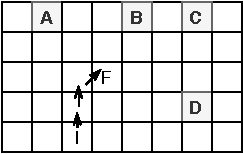
\includegraphics[width=0.5\columnwidth]{img/rg.pdf}
  \caption{The plan recognition problem}
  \label{fig:prp}
\end{figure}

Ramirez and Geffner provides a solution to the recognizer's question by accounting for the cost differences of two types of plans for each goal: (1) plans that reach a goal while going through the observations and (2) plans that reach a goal without going through the observations. Formally,
$\forall g \in \mathcal{G}: \Delta_{g} = C_g(O) - C_g(\overline{\rm O})$, where $\Delta$ refers to the cost difference, $C_g(O)$ refers to the cost of the plan that reaches goal $g$ going through $O$ and $C_g(\overline{\rm O})$ is the cost of the plan that reaches the goal without going through $O$. In the example in Figure~\ref{fig:prp}, when the agent is (\texttt{at F}),\\
$\Delta_{(at A)}= (2+3\sqrt{2}) - (3+\sqrt{2})=1.8$\\
$\Delta_{(at B)}= (3+2\sqrt{2}) - (2+2\sqrt{2})=1$\\
$\Delta_{(at C)}= (6+2\sqrt{2}) - (4\sqrt{2})=3.2$\\
$\Delta_{(at D)}= (4+2\sqrt{2}) - (3+\sqrt{2})=2.4$\\
This indicates that from the given observations, (\texttt{at B}) has the least cost difference. What does that mean? 
According to the $\Delta_g$ formula, if for a specific goal, if $C_g(O)$ is greater, it follows that $\overline{\rm O}$ is more likely than $O$ (because the rational actor agent would follow the lower cost plan). 
Putting it differently, smaller $\Delta$ means that cost of $\overline{\rm O}$ plan is greater, thus the agent is likely following the plan that is aligned with the observations. 
Therefore, given the observations, the most likely goal would be the one that has the least cost difference. 
The solution to the plan recognition problem is expressed as the subset of goals $g\in \mathcal{G}$ such that the \textit{optimal} plan for $g$ satisfies the observation sequence $O$.

How does the recognizer produce plans that are compatible with the observations? 
For this, Ramirez and Geffner use a technique called ``\textit{Compiling Observations Away}''. When the observations are compiled into the domain theory, it forces the automated planner to search for solutions that already contain the observations. 
They transform the original domain (defined in STRIPS) $D$ into a domain $D^\prime$ given the observations $O$. The new domain has the same initial state and actions as $D$. 
However, new state variable predicates are added to $D^\prime$ such that if an action $a$ is in $O$, it's definition in the domain gets added an extra state variable predicate to its post-conditions. 
This modification is done only if $a$ is the first observation in $O$. 
If there is an action $b \in O$ that immediately comes before $a$, then the preconditions of action $a$ gets added a new state variable predicate (that is already in the post conditions of $b$) and post conditions of action $a$ gets added a second new state variable predicate.

Once these modifications are done to the domain definition $D^\prime$, automated planners can be used to find plans that are compatible with the observations. $D$ is used to find plans that are not compatible with the observations. Then, to do the recognition task for each $g\in \mathcal{G}$ they compute the posterior probabilities $P(g|O) \cong \alpha P(O|g) P(g) $, where $P(g)$ is the prior probability for $g$ given as input to the recognition task and $\alpha$ is the normalizing constant. Ramirez and Geffner characterize the likelihood $P(O|g)$ as a Boltzmann distribution $P(O|g)=\frac{e^{-\beta\Delta_g}}{1+e^{-\beta\Delta_g}}$ where $\beta$ is a positive constant and $\Delta_g$ is the cost difference between observation compatible and not compatible plans for goal $g$.

\noindent\textbf{Constraints in the Approach}\\
In order to compute the posterior probabilities over the likely goals, the planner has to be invoked twice: once to find the observation compatible plans and once to find the plans that are not compatible. 
This may be costly for large problems and plan recognition in real time (i.e., when observations arrive incrementally). 
Furthermore, for the two costs to be different (and enable the recognizer to correctly identify the actor's goal) the observations must contain action landmarks for the goal we want to identify.
Landmarks are state predicates that must be true in any valid plan to reach the goal \cite{hoffman2004lm}.
Action landmarks contain the landmarks as their post-conditions. 
If the observed action is an action landmark for $g$, then $C_g{(\overline{\rm O})}$ will be higher and as a result $P(g|O)$ will be higher. If there are many ways to reach $g$ (i.e., no action landmarks) then the cost difference $C_g(O) - C_g{(\overline{\rm O})}$ will not be significantly different and as a result, it will be harder for the recognizer to identify the correct goal. 
A solution that address these constraints is proposed by E-Martin et al., which calculates the \textit{interaction} of two or more actions \cite{yolanda2015} using the \textbf{plan graph} representation of the planning task  \cite{blum1997fast}. 
They first define the cost of two proposition/actions to be established together (\textit{cost interaction}). 
This cost is propagated through the plan graph starting from the initial state until the goal states are achieved. 
The cost of achieving the goal is the sum of interactions between propositions and the costs of actions required to achieve that goal.
Like Ramirez's solution, this work also assumes that the observations are not noisy but may be incomplete.

In certain problems, it maybe difficult to provide reasonable prior probabilities for the likely goals. This is specially true in the kinds of planning domains we are working on in this research, where certain facts about the domain are hidden to the actor and the absence of complete knowledge may enable some unintended goals, regardless of their priors. For example, consider a human user unwittingly falling victim to a phishing scam because he can not recognize phishing web sites from the safe ones.

Furthermore, in certain cases the recognizer may need to recognize the actor's plan before all the observations are made available. This is also an important requirement in the domains we are studying in this research, where an agent needs to assist human users avoid certain undesirable consequences before the human user's task is completed. This requires that recognition needs to happen as observations are made available incrementally. We will discuss some recent work in online recognition in the following sections.

\noindent\textbf{Sohrabi et al. 2016 - Plan Recognition with Unreliable Observations}\\
The recognition task is similar to the probabilistic plan recognition problem proposed by Ramirez and Geffner, where a recognizer receives an observation trace of the actor's agent's behavior and attempts to identify what the actor's plan is. They also use the ``\textit{Compiling Observations Away}'' theory to generate a solution to the plan recognition problem. Sohrabi et al. propose several extensions to prior work where (1) the recognition system can now handle noisy or missing observations and (2) address observations over state variables. Further, the recognizer can identify the actor's plan and goals.

This work defines a \textbf{noisy} observation as an action that can not be explained by actions of a plan for a particular goal. \textbf{Missing} observation is an action that should have been in the observation trace but have not. When the observations are unreliable, the cost difference $C_g(O) - C_g{(\overline{\rm O})}$ will be large and as a result it will underestimate $P(g|O)$. This is because with noise in the trace, either the plan that is compatible with $O$ will have a higher cost than the plan that is not compatible with $O$ or the planner may not be able to find an observation compatible plan. To remedy this situation, they propose a new approach to ``\textit{Compiling Observations Away}'' that modifies the planning domain to include action costs; specifically penalties for noisy/missing observations.

In Ramirez and Geffner's work, the observations are presented as actual actions as defined in the domain theory. Shorabi et al. argue that in realistic examples, it may be difficult for the recognizer to observe the action itself, but he may be able to observe the effect of the action in the state. Therefore, they define the observations over state variables instead of actions. When  ``\textit{Compiling Observations Away}'', they augment the domain $D$ with special ``discard'' and ``explain'' actions. This classification helps to identify noisy observations that must be discarded. The definition for the plan recognition problem $\mathcal{R}$ closely follows from Ramirez and Geffner's definition, where $\mathcal{R}=\langle \mathcal{F}, \mathcal{A}, s_0, \mathcal{G}, O, PROB\rangle$. However, $O$ is now a sequence of states, instead of actions. Recall that the domain theory $D=\langle \mathcal{F}, \mathcal{A}, s_0 \rangle$. The augmented domain theory $D^\prime=\langle \mathcal{F}^\prime, \mathcal{A}^\prime, {s_0}^\prime\rangle$. $\mathcal{F}^\prime$ contains state variable predicates from $D$ plus the new predicates  $done, l_{o_0}$ to signal that the goal state is complete and to indicate the start of the $O$ respectively. 
In addition  $\mathcal{F}^\prime$ has a set of special predicates $l_{o_i}$ for each observation $o_i$ indicating whether the observation was discarded or explained. 
The special predicates ensure the total order of observations is maintained when the new actions are executed. 
${s_0}^\prime$ is equal to $s_0$ and has the additional predicate $l_{o_0}$. Goal $G^\prime \in \mathcal{G}$ are expressed such that $G^\prime = \lbrace done, l_{o_m}\rbrace$, where $l_{o_m}$ is the last observation. There are four types of actions in $\mathcal{A^\prime}$, each having costs associated with them \textbf{goal} action, \textbf{discard} action, \textbf{explain} action and original actions from $\mathcal{A}$. The \textit{goal action} has preconditions equal to the goal state, postcondition equal to $done$ and cost = 0. The \textit{discard action} is added when the observed state is false in the current state (i.e., observation not explained). As the post condition, the discard action adds the special predicate $l_{o_i}$ and removes the special predicate added by previous observation $l_{o_{i-i}}$. Discard action cost = $b_2$ (a application specific weight). The \textit{explain action} is added when the observed state is true in the current state. The post condition is similar to the discard action. The explain action has cost = 0. The \textit{original action} has the same pre/post conditions from the original definition $\mathcal{A}$. However, it is now assigned a new cost, which adds a penalty proportionate to the number of missing observations. The plans derived from the augmented domain theory $D^\prime$, now reflect penalties to missing and unexplained observations.

The recognition task is performed by deriving posterior plan probabilities P($\pi|O$) and posterior goal probabilities P($G|O$) following the same process as Ramirez and Geffner. 
\begin{itemize}
\item $P(\pi|O) = \beta P(O|\pi)P(\pi|G)P(G)$
\item $P(G|O) = \beta P(O|G)P(G) = \beta \sum_{\pi \in \Pi}P(\pi|O)P(G)$
\end{itemize}
$P(G)$ is an input to the recognition problem as $PROB$. Note that, now $P(G|O)$ depends on $P(O|\pi)P(\pi|G)$. Sohrabi et al. approximates this value such that $P(O|\pi)P(\pi|G) \approx 1- \frac{\beta V(\pi)}{\sum_{\pi^\prime \in \Pi}V(\pi^\prime)}$, where $V(\pi)$ is a weighted cost factor that accounts for noisy and missing observations in a plan $\pi$ for goal $G$ that satisfies $O$.  The term $\sum_{\pi^\prime \in \Pi}V(\pi^\prime)$ is computed from the sampled plans that are derived from the augmented domain theory $D^\prime$ using Top-K planner \cite{riabov2014}, which finds k-best plans and using diverse plans. The recognized goal/plan is the goal/plan that has the highest posterior probability from the set of most likely goals/plans.

\noindent\textbf{Constraints in the Approach}\\
Similar to Ramirez and Geffner's work, this solution for plan and goal recognition relies on being able to provide the goal priors as an input to the algorithm. Furthermore, the observations (although given as a sequence of states) need to be provided to the algorithm up front. For the assistive agent we are designing for human users, the recognition process needs to be separated from these constraints.

\subsection{Shvo et al. 2018 - Multi-agent Plan Recognition}
So far, we have only discussed plan recognition in situations where there is one actor and one recognizer. An extension to this paradigm is proposed in work by Shvo et al. \citeyear{shvo2018}, where the Multi-agent Plan Recognition problem (MAPR) is introduced. In MAPR the recognizer infers the goals and plans of multiple agents. The observations given to the recognizer originates from many agents. MAPR has interesting applications in multiple real domains such as intrusion detection, surveillance and so on.

When performing MAPR, the recognizer takes into account different capabilities of the agents in the domain. In addition, this work further considers actions taking some time to finish executing (durative actions). Similar to the work by Shorabi et al., observations are processed as states and not as actions. Furthermore, observations may be unreliable (i.e., contains missing/unexplainable observations). This solution to MAPR problem also builds on the plan recognition approach proposed by Ramirez and Geffner that proposes modifications to the domain theory to recognize goals/plans using automated planners. In the first step, the multi-agent aspect is compiled away into the domain theory. When there are many agents in the environment having different actions that they can execute, some actions can be executed concurrently, while others can not. They use temporal nature of actions to establish ordering constraints on the actions.  Two special state predicates are defined for actions that operate as \textit{action delimiters}: ``start'' and ``end'', which specify the pre and post conditions to the temporal action respectively. Additionally, they also define an overall precondition to the temporal action, which must hold true in every state between the ``start'' and ``end'' states. When actions are temporal, the solution plan is a sequence of action-time pairs showing actions that can execute at the same time when they are applicable.  Use of temporal actions allows concurrency of the agent's own actions as well as actions of different agents. Now, in order to compile away the multi-agent aspect, they define a privacy model for the agents when executing the temporal (and perhaps shared) actions. Action $a$ can be executed by agent $i$ if and only if $a$ is private to agent $i$ or is public to all agents. This is done by introducing special predicates to track the ownership (i.e., which agent, what objects) of state variables when a temporal action is being executed. This privacy model is added to the initial state of the planning problem. The second step is ``\textit{Compiling Observations Away}''. Here, they follow the same process as Sohrabi et al. 2016 to ``\textit{Compiling Observations Away}'' for missing and noisy observations. Then, the plan recognition problem becomes finding the posterior probabilities of plans P($\pi|O$) and  goals P($G|O$). Because the domain theory now has temporal actions, it is possible to use temporal planners to find sample solution plans.

\noindent\textbf{Constraints in the Approach}\\
The proposed approach is only evaluated for a case where the agents pursue one common goal. The assistive recognizer agent we are presenting in our research is an extension to this work. When different agents pursue different and competing goals, and when the recognizer is expected to assist one agent in the environment it needs to consider how likely the goal of the agent (who is being helped) will be threatened by competing agent(s) actions. The recognizer agent must be  able to complete recognition \textit{in time} to identify when a partial plan that seems to be helpful can be subverted by a competing agent during execution and alert the agent accordingly.



\subsection{Planning as a Tool to Model User Behavior in Cyber-security}
Cyber-security domain offers a lot of promise to study behavior both as normal users and as adversaries in automated planning. Behavioral Adversary Modeling System (BAMS) \cite{boddy2005course} uses automated planning to help computer network administrators in analyzing vulnerabilities in their system against various kinds of attacks. BAMS takes into account the properties of an adversary and produces plans that lead to system exploits that also coincides with the adversary model. While this work does not directly apply to plan recognition at its core, it illustrates a use case where classical planning can be used to design assistive systems targeted towards human end users.

This work models network vulnerabilities of a document management system as a planning problem and integrates a predictive behavior model of an adversary (who is a malicious insider) so that network administrators can concentrate on hardening the system in places where exploits are most likely and result of the exploit will be most costly. The network security planning domain contains objects such as email messages, files, hosts, user identifiers etc. and has 124 predicates to represents facts about the environment, status of tiles, capabilities, vulnerabilities of programs, knowledge possessed by users etc. Actions are represented in STRIPS with parameters, pre and post conditions. The domain has 56 actions that capture system events such as document accesses, user group modifications etc. The adversary's objectives are specified in the planning problem as goals. They use an off-the-shelf planner Metric-FF  \cite{hoffman2003ff} to find possible plans of the adversary. A graphical user interface allows end-users (i.e., network administrators) to configure problem specifications (hosts in the system, access control rules etc) and the attacker's properties (skills/tools he has) without having to encode them in PDDL.

The authors highlight several issues in modeling expressive scenarios in PDDL. 
The first constraint is the difference between the level of detail that is required in the domain and what can be modeled in the planning language. If the representation is too detailed, the resulting plans will be uninteresting and difficult for the users to extract information. Furthermore, developing and maintaining these highly descriptive domains will be a difficult task requiring expert knowledge. The second constraint is providing the plans generated by the automated planner to end-users in a natural representation. PDDL plans are not naturally comprehensible to end-users. The authors propose an encoding scheme for the PDDL actions and providing explanatory texts to capture state transitions that take place within the solution plan.

In this dissertation, we take a step toward designing assistive systems using automated planning to help human end users, who are non-experts (e.g., home users). 
Home users are specially vulnerable to undesirable consequences because they lack the know-how to recognize risky situations in advance.
A previous study \cite{byrne2016} showed that home users pay more attention to the benefits of the activities than the risk; they have goals that they want/need to achieve and are willing to take the risk to achieve them. Many triggering actions may be normal
activities (e.g., reading email, clicking on links) with the user more focused on the goal than on the risk. Thus, the undesirable consequence recognition problem needs to take into account the user’s intention as well as the undesirable consequence.

Howe et al. \citeyear{howe2012psychology} observed that most studies that look into computer security practices of users relying on self reported surveys suffered from issues such as respondent bias, socially desirable responding and peer perception.
The authors posited that experiments based on simulation, which place the participant in the actual situation that is monitored can help reduce such issues and also be leveraged to assess the emotional reactions of users to interventions and warnings.

The Intervention Problem can be directly applied in the cyber-security domain.
An attacker attempting trick the user into compromising his security/privacy during day-to-day computing tasks fits the model of the competitor we discussed in this work.
The attacker creates opportunities for phishing and malware attacks by making them to appear as common harmless tasks such as email and installing software. 
Unable to recognize these attacks in advance, the user becomes an unwitting accomplice to security breaches.


\section{Goal Recognition}
Similar to plan recognition, early goal recognition solutions involved using plan libraries. Lesh and Etzioni \citeyear{lesh1996} use a plan library based approach for goal recognition. Here, they use a data structure called a \textit{consistency graph}, which is a directed graph with actions, action schema, and goals as nodes. There is an edge between two nodes if there is a \textit{consistent} plan that supports the two nodes for some goal. Their approach to recognizing an actor's goal rely on quickly determining if a goal is inconsistent with the observed actions. Informally, the recognizer needs to conclude that the actor could not possibly have executed the observed actions as a part of a plan to satisfy the goal. This requires the recognizer to reason about \textbf{all} plans for each candidate goal. Consistency graph is an efficient way to represent planning problems and reason about them tractably.

Similar to the plan recognition problem, the goal recognizer takes as input a set of likely goals, a sequence of actions executed by the actor, actor's beliefs and a model of action schema that can be executed in the domain. The solution to the goal recognition problem is a subset of the goal schema such that, for every element in the subset, there exists a plan that achieves that goal. In order to find this goal schema subset, they first build the consistency graph. Then they gradually remove elements (action schemas/goal schemas) following a predefined rule set, which recognizes elements in the graph that are not in any consistent plan without violating the graph correctness.

Actions are removed from the consistency graph when the observed action is not consistent with other actions in the plan or the goal. This rule is sensitive to noisy observations. Oftentimes, human users do not take actions to achieve a goal in a rigid sequence. For example, they may try a few options before settling into one plan or they could just be \textit{exploring} the domain. This is specially true in the kinds of domains we are investigating in this research: cyber-security and Rush Hour. Actions generated in these type of situations may eventually be removed from the graph, which results in the recognizer failing to identify the actor's goal.

\subsection{Ramirez et al. 2009 - Plan Recognition as Planning}
This work is the precursor to the probabilistic plan recognition work proposed by Ramirez and Geffner that we discussed in plan recognition related work. There are many similarities between plan recognition as planning \cite{ramirez2009plan} and probabilistic plan recognition. As stated in the previous work by the same researchers, the environment $E$ and the recognizer's problem are defined the same. They both use the domain theory to generate two types of plans to find the most likely goal: (1) one that is compatible with observations and (2) one that is not compatible with observations.
The key differences are the assumption that the actor is only executing optimal plans and the approach they use to compile the observations away. The ``\textit{Compiling Observations Away}'' technique used in this work to modify the original domain theory $D$ into a new domain theory $D^\prime$ by adding new action definitions and predicates corresponding to the observations.

Let us define $D = \lbrace \mathcal{F}, \mathcal{A}, s_0 \rbrace$ for plan recognition problem illustrated in Figure~\ref{fig:prp}. $\mathcal{F}= \lbrace (at\:x), (adj\:x,\:y), L1\_1, L1\_2, \ldots, L8\_5\rbrace$, which indicates that the actor is at location $x$ and location $x$ is adjacent to location $y$ respectively. Predicates $L1\_1$ etc. refer to the cells on the grid, corresponding to the row and the column numbers of the cell. $\mathcal{A}= \lbrace move(x,y)\rbrace$, which indicates that the agent can move from location $x$ to location $y$. Preconditions of the move operation $pre(move)=\lbrace (at\:x)  \land  (adj\:x,\:y) \rbrace$. Post-conditions for the move operation $add(move)=\lbrace (at\:y) \rbrace$, $del(move)=\lbrace (at\:x) \rbrace$. The initial state $s_0=\lbrace (at\:L5\_3)\rbrace$. Let us assume the recognizer gets the observation trace $O=\lbrace move(L5\_3, L4\_3)\rbrace$, which indicates that the actor has moved up one cell from the initial position.

\sloppy
If we are to apply the \textit{Compiling Observations Away} theory proposed by Ramirez and Geffner to transform $D$ to $D^\prime=\lbrace \mathcal{F}^\prime, \mathcal{A}^\prime, {s_0}^\prime\rbrace$ adds one new state variable predicate such that $\mathcal{F}^\prime=\mathcal{F}\cup\lbrace p_{move(L5\_3, L4\_3)}\rbrace$ and one new action such that $\mathcal{A}^\prime=\mathcal{A}\cup\lbrace ob_{move(L5\_3, L4\_3)}\rbrace$. The new state variable predicate indicates that the an observation has occurred in the environment (in this case, move up). The new action is fully grounded and defined below.\\
\textbf{operator:} $\texttt{ob}_{\texttt{move}(L5\_3, L4\_3)}$\\
\textbf{preconditions:} $\lbrace$ (\texttt{at}$\:L5\_3$) $\land$  (\texttt{adj}$\:\:L5\_3$,$\:L4\_3$) $\rbrace$ \\
\textbf{postconditions:} $\lbrace$ $\neg$ (\texttt{at}$\:L5\_3$) $\land $ (\texttt{at}$\:L4\_3$) $\land$ $\texttt{p}_{\texttt{move}(L5\_3, L4\_3)}$ $\rbrace$\\
Comparing this to the compilation proposed in probabilistic plan recognition, the probabilistic method does not add any new action definitions to the domain theory. Instead, only the new state variable predicates are added into existing action definitions. In order to force the planner (an optimal planner in this case) to find solutions that are optimal in number of moves and also contains actions in the observations, the goals $\mathcal{G}$ are also modified to reflect the effects of the observation. For example, the goal $g \in \mathcal{G}$ such that $g=\lbrace$(\texttt{at}$\:L1\_2$)$\rbrace$ is modified to  $g^\prime=\lbrace$(\texttt{at}$\:L1\_2$)$ \:\land\: \texttt{p}_{\texttt{move}(L5\_3, L4\_3)}\rbrace$. The process of adding new state variable predicates and new actions is repeated for all actions in the observation trace. All goals in the candidate goal set are also modified accordingly. The likely goal given observations ($P(g|O)$) is found by the same calculation as the probabilistic plan recognition by taking the cost difference between optimal plans that contain the observations and optimal plans that do not contain the observations.


\noindent\textbf{Constraints in the Approach}\\
This work also has the same constraints as the probabilistic plan recognition, in that the goals are recognized when all the observations are available and the difficulty in specifying the goal priors. Plan intervention requires us to identify undesirable consequences before the task is completed. It follows that the offline model of recognition is not suitable for plan intervention. However, we will use the plan recognition with ``\textit{Compiling Observations Away}'' theory to benchmark our initial plan intervention solutions.


\subsection{Vered et al. 2017 - Online Goal Recognition in Continuous Domains}
So far, the goal and plan recognition problems we have discussed in this chapter assume the actor and the recognizer are in a discrete domain and the observations are discrete. Online goal recognition \cite{vered2017} extends the recognition problem to continuous domains. For example, in robot motion planning, we can define a simple domain as the space of possible positions for a robot. This definition can further be extended to define higher order dimensions such as angle, velocity etc. Further, the recognition is online, which means that the recognition problem must be solved for every new observation when they are revealed. The recognizer receives observations of the actor's position in the same n-dimensional space (e.g., a point or a trajectory). The recognition problem them becomes finding the goal $g$ in the candidate set of goals $\mathcal{G}$ that best matches the observations. Formally, we seek to determine $P(g|O)$ for each goal $g\in \mathcal{G}$. The recognized goal is the one that has the highest posterior probability.

They propose a new method for ranking goals in $\mathcal{G}$. Instead of taking the cost difference (Ramirez and Geffners' approach) they define a ratio $score(g)=\frac{cost(i_g)}{cost(m_g)}$, where $i_g$ is the \textit{optimal} plan to achieve $g$ and $m_g$ is the \textit{optimal} plan that achieves $g$ and includes all the observations. When the optimal plan that has all the observations is the same cost as the optimal the score approaches 1. Then $P(g|O) = \eta score(g)$, where $\eta$ is the normalizing constant. $i_g$ can be computed using a planner. To compute $m_g$, they exploit the fact that each observation is a trajectory or point in the continuous space and each likely plan is also a trajectory in the same space. Therefore $m_g= prefix + suffix$, where $prefix$ is built by concatenating all observations in $O$ into a single trajectory, and the $suffix$ is generated by calling a planner from the last observed point to goal $g$. To improve the computation efficiency during recognition, they introduce two functions: RECOMPUTE - recomputes the new plans only if the new observations seem to change the plan significantly, and PRUNE - removes unlikely goals from $\mathcal{G}$.

\noindent\textbf{Constraints in the Approach}\\
Although the recognition algorithm is evaluated in continuous domains, follow up work extends this solution to discrete domains \cite{vered2018goalrec}. The planning applications we are studying in this research are modeled for discrete domains. We will use goal ranking heuristic proposed in this solution to benchmark our initial plan intervention solutions.

The proposed online goal recognition approach further reduces the computational cost by introducing \textit{landmarks} to prune the likely goals \cite{vered2018goalrec}. 
Landmarks are facts/actions that must be true/executed at some pin all valid plans that achieve a goal from an initial state \cite{hoffman2004lm}. 
This work uses landmarks to heuristically estimate the goal completion ratio (i.e., more landmarks are active in the current state means that particular goal is closer to being achieved) as a proxy for estimating $P(g|O)$. Landmark based heuristics are often times used to improve run time during the goal recognition process. Pereira et al. use a landmark based heuristic to estimate the proximity to each goal \cite{pereira2017}. This heuristic measures the ratio between achieved and non-achieved landmarks.


\section{Recognition and Interaction}
In the goal/plan recognition  work discussed so far, the recognizer passively observes the actor. The recognizer's task finishes once the actor's goal/plan is identified. An extension to this model is to allow the recognizer to interact with the environment and affect the actor's behavior. This interaction can be \textbf{offline}: where the recognizer modifies the domain before the actor can execute any plans on it, \textbf{online}: provoke the actor to behave in some specific way by setting values of environment features, and \textbf{direct communication}: where the actor is asked questions such that the goal hypotheses can be pruned quickly. 

When designing assistive intervention models for human users, in addition to recognizing what they are trying to achieve in the domain, we must provide some guidance if it can be determined that the goal they are trying to accomplish has become unachievable. Prior work in goal/plan recognition provide some insight on how this can be achieved by allowing the recognizer to interact with the actor. We discuss some approaches below.

\subsection{Keren et al. 2014 - Goal Recognition Design}
Goal recognition design (GRD) \cite{keren2014grd} proposes a solution that allows the observer to measure the ``difficulty'' of performing goal recognition in the current domain and propose modifications (e.g. blocking actions) such that goal recognition can be done easily. GRD is an offline interaction activity, which means that unlike the typical plan/goal recognition that relies on having an observation trace for the actor's behavior, GRD analyzes the plans for possible goals in the domain an actor might execute and evaluates how distinct the plans are.

This work introduces a new metric \textit{worst-case distinctiveness} (\textit{wcd}) that measures the maximum length of the common prefix all plans for the likely set of goals may share in the current design of the domain. The solution to the GRD problem is a modified domain that assures \textit{wcd} is minimized, when plans are generated optimally. It also assumes that the actions are deterministic and fully observable.

\subsection{Pozanco et al. 2018 - Counterplanning using Goal Recognition and Landmarks}
In multi-agent settings the agents in the domain may be adversarial. This means that the agent may want to prevent another agent from achieving its goal. 
This work presents a domain independent approach for counterplanning based on goal recognition, landmarks and automated planning. 
The design of the counterplanning domain is such that there are two adversarial agents (seeking agent and preventing agent). 
The two agents pursue different goals. 
The recognizer's task is to help the preventing agent block the seeking agent from reaching his goal.

Counterplanning requires that the recognizer quickly identify the seeking agent's goal. 
This work uses Ramirez and Geffener's probabilistic goal recognition algorithm to perform goal recognition. 
Next, the recognizer needs to identify the earliest landmark for the seeking agent's planning problem (for the recognized goal) that needs to be blocked (i.e., counterplanning landmark). 
A counterplanning landmark is given a set of fact landmarks from the seeking agent's planning task, the counter planning landmark is a postcondition of an action the preventive agent can execute.
If the counterplanning landmark is a positive fluent, the preventive agent's action must delete it.
If the counterplanning landmark is a negative fluent, the preventive agent's action must add it.
The recognizer's interaction occurs when he uses automated planning to generate a plan to achieve the counterplanning landmark (e.g., negating the landmark), and therefore blocking the seeking agent's goal achievement.

\subsection{Mirsky et al. 2016 - Sequential Plan Recognition}
In goal recognition, the recognizer reasons about how likely a given set of possible goals are given the actor's behavior. The recognizer's task may fail if he can not accurately disambiguate between possible goal hypotheses. This work proposes a solution that involves the recognizer querying the actor about whether a candidate plan in one of the goal hypotheses matches the actor's intention. During the recognition process, the actor is sequentially queried in real-time whether the observed partial plan is correct. The actor's answers are used to prune the possible hypotheses, while accounting for the incomplete plans that could match with the observations after several other observations happen in the future. In order to optimize the querying process, the recognizer considers only the queries that maximizes the information-gain and the likelihood of the resulting hypotheses given the expected query result.

This solution assumes that a plan library is provided to the recognizer in advance. Their implementation of the plan library uses trees to represent the possible plans for goal hypotheses. The planning domain used in this study describes how to perform chemistry lab experiments  using an educational software that simulated a virtual lab. The plans in the planning library were traces were taken from real students' traces when interacting with the virtual chemistry lab.


\section{Behavior Classification}
The design of assistive agents for human users require that the recognizer be able to identify human behavior and how well the  behavior aligns with the goals of the system they interacts with. Human users are not always rational and may have hidden goals. It maybe an unfair comparison to model them as rational agents in real life scenarios.
 
Behavior classification is different from typical plan/goal recognition. 
It aims to achieve some insight about the actor from the passive observer's perspective. The work proposed by Borrajo et al. \citeyear{borrajo2020domainindependent} discusses the design of an observer agent, which tries to learn characteristics of other agents by observing their behavior when executing actions in a given environment. 
Using the financial transactions domain as a case study, this work models two agents: the actor (e.g., a bank customer) and an observer (e.g., the banking institution). Only the actor can execute plans in the environment. The observer does not know the actor's goal and has partial observability of the actor's behavior (actions the actor executes). Then, the observer's task is to classify the observed behavior into different types of known behavior classes. In order for the application to be domain-independent, the authors use plan distance measures (e.g., Jaccard similarity) between observed actions and distance between observed states as features to train the classifier.
Given two plans $p$ and $p^\prime$, the Jaccard similarity for the actions in the plan is defined as: 
$\frac{\left | A(p)\cap A(p^\prime) \right |}{\left | A(p)\cup A(p^\prime) \right |}$, where $A(p)$ and  $A(p^\prime)$ refer to the sets of actions in the plans $p$ and $p^\prime$ respectively.
We use a similar features to recognize the actor's plan prefixes that lead to undesirable states.



\chapter{Intervention as Planning}
We now discuss our first contribution to recognition.
We show that using automated planning, we can extract features that can differentiate between desirable (helpful) plans and undesirable (unhelpful) plans and remove the dependency on prior probabilities of likely goals in the goal/plan recognition solutions. Our first algorithm re-frames the recognition problem as a classification problem and we study the effectiveness of off-the-shelf classifiers in recognizing helpful plan prefixes.


\section*{Introduction}
\label{sec:intro}
Even the best plan can go wrong.
Dangers might arise from a user failing to follow the plan correctly or as a result of a nefarious agent.
Consider route planning where a driver was unaware of upcoming road damage or a traffic jam.  
Or consider cybersecurity where a user was unaware of an unsafe hyperlink.
In both, plans achieving the desirable goal might have similar prefixes to those that result in undesirable outcomes; only the plan suffix differs.
State-of-the-art plan recognition techniques only provide a part of the solution for selecting interventions.

In this work, we create a domain-independent formulation of learning \emph{whether} to intervene.
At a minimum, intervention problems require a user and some intervening observer.
In other settings, the observer also considers actions of a competing agent.
The user and the competing agent have partial visibility and can not recognize the effects of certain actions that take place in the environment.
The user and the competitor (if present) take turns in proposing actions to the observer. The observer evaluates how critical the presented action is for the user to reach his goal while avoiding the undesirable state using  domain-independent features. If the observer finds that the presented action is critical, then it is flagged to warn the user. We discuss two types of actions that must be flagged: direct and indirect. Direct contributing actions have the undesirable state as their post-condition. Indirect contributing actions are sequences that add the necessary conditions leading to the undesirable state.


The contributions of the work discussed in this chapter include:
\begin{itemize}
\item extending an existing plan recognition model to the intervention problem and demonstrating that three state-of-the-art approaches do not perform well for this problem
\item formalizing the online intervention problem as determining when the criticality--i.e., the opportunity or urgency of possible damage--of a state warrants interruption; 
\item modeling the observer's decision space as an \emph{Intervention Graph}, which can be constructed explicitly or sampled with the TopK planner (Riabov et al., \citeyear{riabov2014});
\item defining domain-\emph{independent} features to assess the criticality of a state using the Intervention Graph;
\item extending existing goal/plan recognition benchmarks \cite{ramirez2009plan,ramirez2010probabilistic} to incorporate intervention and introducing a new plan intervention benchmark domain called Rush Hour, 
\item adapting four algorithms that learn whether to intervene, 
\end{itemize}
Our results show that the proposed intervention solution  outperforms existing plan recognition algorithms with fewer false positives and false negatives.

Ram\section*{Intervention Example}
Consider an example where a user present actions while an observer decides whether to intervene.
The observer is interested in two kinds of states:  a desirable state $\mathrm{d} \subseteq F$ is the user's goal and the undesirable state $\mathrm{u} \subseteq F$  is an outcome the user wants to avoid, but may not be able to detect.
(For convenience, we may discuss $\mathrm{d}$ or $\mathrm{u}$ as single states even though they are sets.)
The observer's objective is to help the user achieve $\mathrm{d}$ while avoiding $\mathrm{u}$.
Thus the observer must identify actions that lead to $\mathrm{u}$ and intervene when appropriate.

Figure~\ref{fig:single} shows a grid navigation task where the user navigates from \texttt{w1} by moving vertically and horizontally and \texttt{y3} contains a pit the user can not see.
Thus, \mbox{$\mathrm{d}=$ \texttt{at(z3)}} and \mbox{$\mathrm{u}=$ \texttt{at(y3)}}. The user computes a satisficing plan for $\mathrm{d}$ and reveals by presenting an action at a time to the observer. A, B, C are all feasible from the user's perspective.
However, the observer knows plans B and C are unsafe.
If the user presents actions \texttt{move(y2,y3)} or \texttt{move(x3,y3)} observer must flag them because they are direct contributors to $\mathrm{u}$.
If the user is executing an optimal plan, the observer can flag indirect contributors to $\mathrm{u}$. In this case, if the action \texttt{move(w2,w3)} is revealed, it must be flagged because the user can only move up to reach $\mathrm{d}$ (without violating optimality). Thus $\mathrm{u}$ becomes inevitable. Also, \texttt{move(w3,x3)}, \texttt{move(x3,y3)} must be flagged. We formally define the terms \textit{directly contributing action} and \textit{indirectly contributing sequence} later.

Interrupting the presented actions directly nor indirectly contributing to $\mathrm{u}$ results in false alarms.
We tune the intervention sensitivity; i.e., direct vs. indirect using a set of intervention features defined in Section~\ref{sec:features}.
But next we consider how to formulate intervention as an extension of plan recognition.

\begin{figure}[ptb]
        \centering{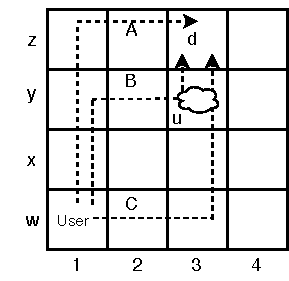
\includegraphics[width=0.5\columnwidth]{img/single.pdf}}
         \vspace{-1em}
        \caption{An example of helpful intervention.}
        \vspace{-1em}
        \label{fig:single}
\end{figure}
%
%%=========================================================================
%%=========================================================================
%%=== problem
%%=========================================================================
%%=========================================================================
%
\section*{Intervention as Planning}
\label{sec:intervention}
We develop an approach whereby plans leading to $\mathrm{u}$ or $\mathrm{d}$ are identified using the recognition approach advanced by Ramirez and Geffner (2009, 2010).
The observer should allow the user to pursue plans leading to $\mathrm{d}$ and intervene when the user takes actions from plans that get ``too close'' to $\mathrm{u}$.
Our key insight is considering $\mathrm{u}$ as a ``goal'', which is justified for planning where we want to identify plan suffixes that lead to undesirable outcomes. 
Undesirable plans $\Pi_{\mathrm{u}}$ are plans that achieve $\mathrm{u}$ and desirable plans $\Pi_{\mathrm{d}}$ achieve $\mathrm{d}$. 
Thus, the observer must consider the two states together $\mathcal{G}=\lbrace\mathrm{u} \cup \mathrm{d}\rbrace$
The observer's recognition problem is: in domain $D$, given $O = \lbrace o_1, \ldots o_{i-1}\rbrace$, what is the most likely ``goal'' from $\mathcal{G}$ if $o_i$ will be observed? 
Plan recognition algorithms should help the observer identify the most likely goal and intervene if $\mathrm{u}$ is most likely.
When $\mathrm{u}$ and $\mathrm{d}$ are far apart, recognition is straightforward.
When they are proximate, it is difficult for the observer to recognize $\mathrm{u}$ on time.

In intervention, the observer asks the question: in domain $D$, given $O = \lbrace o_1, \ldots o_{i-1}\rbrace$ must $o_i$ be flagged to prevent reaching $\mathrm{u}$ first?
Note that $O\not\models\mathrm{u}$. 
If we are to solve intervention as a plan recognition problem, we need to assume a prior probability (e.g., uniform) over $\mathcal{G}$. Sometimes, it may be hard for the observer to correctly determine the priors. From the user's point of view, the prior of $\mathrm{u}$ $\approx 0$ because he does not know about it, whereas the observer may assign a different prior. This leads to false alarms/misses if intervention happens based on the most likely goal given $O$.


\theoremstyle{definition}
\begin{definition}
The \textnormal{online plan intervention problem} is a tuple $\mathcal{I} = \langle D, O, \mathcal{G} \rangle$ where $D=\langle F, A, I \rangle$ is a planning domain, 
$O$ is  sequence of observed actions ($o_1, o_2, \ldots o_{i-1}$), $o_1$ is the presented, new action, $\mathrm{d},\mathrm{u} \in \mathcal{G}$ and $\mathcal{G} \subseteq F$
\end{definition}
The user solves the planning problem $P_0=\langle F_0, A_0, I_0,\mathrm{d}\rangle$, where $F_0 \subset F$, $A_0\subseteq A$, $I_0 \subseteq I$ and $\mathrm{d}\subset F$. 
Because $\mathrm{u}\subset F$, $\mathrm{u}\neq \mathrm{d}$ and $\mathrm{u}$ is hidden to the user, some solutions to $P_0$ become undesirable. Therefore, the observer can partition the solution space for $P_0$ to two disjoint plan sets: desirable ($\Pi_{\mathrm{d}}$), which do not contain actions that lead to $\mathrm{u}$ and undesirable ($\Pi_{\mathrm{u}}$). The user following his own plan may present actions to the observer from both $\Pi_{\mathrm{u}}$ and $\Pi_{\mathrm{d}}$. 

A solution to $\mathcal{I}$ is a binary decision that maps the current plan prefix, including the action the user presents $\lbrace O\cup o_i\rbrace$ to $\lbrace Yes,No\rbrace$ indicating whether it requires intervention. For example, suppose in Figure~\ref{fig:single} the user is executing the plan C $=\lbrace$ \texttt{move(w1,w2)}, \texttt{move(w2,w3)}, \texttt{move(w3,x3)}, \texttt{move(x3,y3)},$\ldots \rbrace$. When he presents \texttt{move(w1,w2)} it is flagged as $No$, when \texttt{move(w2,w3)} is presented, the prefix $\lbrace$ \texttt{move(w1,w2)}, \texttt{move(w2,w3)}$\rbrace$ flagged as $No$ and so on.


We use machine learning to derive functions that perform the mapping from plan prefixes to flagging decisions $\lbrace Yes, No\rbrace$, for an application specific constant $\Theta\mapsto\lbrace$`direct',`indirect'$\rbrace$.
The first method uses features derived from a data structure called an \textit{Intervention Graph}. 
The second method uses plan distance metrics that compare distances between the user's projected plan to $\Pi_{\mathrm{u}}$ and $\Pi_{\mathrm{d}}$ as features. When $\Theta=direct$, we define the directly contributing prefix.
\begin{definition}
A \textnormal{directly contributing action} $a_{crit}$ occurs in an undesirable plan $\pi_{\mathrm{u}}\in \Pi_{\mathrm{u}}$ and execution of $a_{crit}$ in state $s$ results in a state $s^\prime$ such that $s^\prime\models \mathrm{u}$. Directly contributing prefix is such that $\lbrace O\cup c\rbrace$, where $c\in a_{crit}$
\end{definition}
\noindent When $\Theta=indirect$, we define an indirectly contributing sequence $q_{crit}$.
\begin{definition}
An \textnormal{indirectly contributing sequence} $q_{crit}$ is a totally ordered action sequence that starts with the presented action $o_i$ from in an undesirable plan $\pi_{\mathrm{u}}\in \Pi_{\mathrm{u}}$. An indirectly contributing prefix is $\lbrace O\cup q\rbrace $ where $q\in q_{crit}$. Executing actions in any indirectly contributing prefix from state $s$ results in a state $s^\prime$ such that $s^\prime\models \mathrm{u}$. 
\end{definition}

%%=========================================================================
%%=========================================================================
%%===  example
%%=========================================================================
%%=========================================================================
\section*{Intervention With a ``Competitor''}
\label{sec:example}
Above, we introduced the simple version of the intervention problem.
But sometimes there is another agent interacting with the environment at the same time as the user.
We introduce an additional actor, the \textit{competitor}. 
The competitor is not a standard adversary like you would find in a two-player game.
The competitor has a limited set of actions, which he uses to create states that will lead to $\mathrm{u}$ before $\mathrm{d}$ is reached. 

Figure \ref{fig:multi} shows examples with the competitor in a modified version of the block-words domain used in \cite{ramirez2009plan}.
Figure \ref{fig:multi} (top) shows a problem with 4 blocks (T, B, A, D) initially on the table and time flows from left to right. 
$\mathrm{d}=\lbrace$(\texttt{CLEAR T})(\texttt{ON T A})(\texttt{ON A D})(\texttt{ONTABLE D})$\rbrace$(i.e., TAD) and $\mathrm{u}=\lbrace$(\texttt{CLEAR B})(\texttt{ON B A})(\texttt{ON A D})(\texttt{ONTABLE D})$\rbrace$ (i.e., BAD).
The user does not know about the competitor's modifying the state of block B (dotted line block) nor about $\mathrm{u}$. The competitor can only modify the state of block B, and execute actions with the hidden block (stack B, pickup B etc.).
The user may enable $\mathrm{d}$ with the action \texttt{stack(user,A,D)} and at the same time creating an opportunity for the competitor to reach $\mathrm{u}$ first. 
$a_{crit}=\lbrace$\texttt{stack(competitor,B,A)}$\rbrace$. 
$q_{crit}$=$\lbrace$\texttt{pickup(competitor,B)}, \texttt{stack(competitor,B,A)}$\rbrace$.

In Figure \ref{fig:multi}~(bottom) $\mathrm{d}= $ (CUP) and $\mathrm{u}= $ (CUT) are defined the same way as the TAD/BAD example. Block T is hidden from the user. Intervention must happen when \texttt{STACK(competitor, T, P)} is observed. If not, the user could unwittingly reach $\mathrm{u}$ by placing U on T (thinking P is free) and stacking C on U. 
Therefore, $q_{crit}=\lbrace$\texttt{stack(competitor,T,P)}, \texttt{pickup(user,U)},\\ \texttt{stack(user,U,T)}, \texttt{pickup(user,C)},\texttt{stack(user,C,U)}$\rbrace$.

\begin{figure}[t]
          \centering{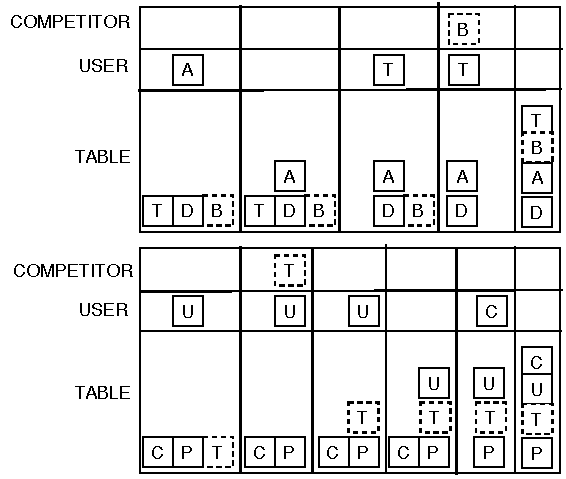
\includegraphics[width=0.5\columnwidth]{img/blocks.pdf}}
                  \vspace{-1em}
        \caption{Reaching $\mathrm{u}= $ (BAD) (top) and $\mathrm{u}= $ (CUT) (bottom) with an competitor and a user.  The table initially contains all four blocks in each example. A block in the user or competitor row indicates a pickup action that is removed using a stack action.}
        \vspace{-1em}
        \label{fig:multi}
\end{figure}

\begin{definition}
The \textnormal{online plan intervention problem} with a competitor is a tuple $\mathcal{I} = \langle D, O, \mathcal{G} \rangle$ where $D=\langle F_0\cup F_1, A_0\cup A_1, I \rangle$ is a planning domain, 
$O$ is  sequence of observed actions, $\mathrm{d},\mathrm{u} \in \mathcal{G}$ and 
$\mathrm{d}, \mathrm{u} \subseteq F_0\cup F_1$
\end{definition}
The user solves the planning problem $P_0=\langle F_0, A_0, I,\mathrm{d}\rangle$.
The competitor wants to solve the planning problem $P_1=\langle F_1, A_1, I,\mathrm{u}\rangle$.
However, the competitor does not have access to all the actions needed to achieve $\mathrm{u}$ and requires the user to enable some conditions for $\mathrm{u}$. Also, $A_1 \cap A_0=\emptyset$ and $F_1 \neq F_0$. Because $\mathrm{u}$ is hidden to the user, some solutions to $P_0$ become undesirable.
Observations for $\mathcal{I}$, contain actions from $A_0$ and $A_1$.
 

Given an observation trace $O = \lbrace o_1, o_2,\ldots o_{i-1}\rbrace$, the observer sees the effects of the actions upto $o_{i-1}$. An intervention episode is defined from state $I$ until one of $\mathrm{u}$ or $\mathrm{d}$ is satisfied. If the competitor is present, which agent presents first action in the episode is decided randomly. The observer makes the intervention decision for the presented action and adds it as $o_{i}$. The agents take turns in presenting the next action $a_{i+1}$ to execute in the episode from $A_0$ and $A_1$ until the episode terminates.
We make several assumptions.
\textbf{(Observability)} 
The observer has full observability, knows about  $\mathrm{d}$ and $\mathrm{u}$ and helps the user avoid $\mathrm{u}$. $\mathrm{u}$ is unknown to the user. $\mathrm{d}$ is unknown to the competitor (if present).
The user can not recognize effects of the competitor's (if present) actions. 
\textbf{(Plans)} 
The user follows a satisficing plan to reach $\mathrm{d}$, but may reach $\mathrm{u}$ unwittingly. 
There is a satisficing plan to reach $\mathrm{u}$ and we assume that it has a common prefix with a plan to reach $\mathrm{d}$. In this work, we are only interested in correctly identifying actions that are in $a_{crit}$ and $q_{crit}$ for a given intervention problem. Therefore, we assume that  the user continues to present the observer with actions from his original plan even after the first positive flag and does not replan. We leave the problem of handling positive flags to future work.
\textbf{(Competitor)}
When present, the competitor only perform actions using objects hidden to the user; this restriction follows from many security domains where an attacker is a remote entity that plants traps and expects the user to become an unwitting accomplice (e.g., attacker sends click-bait phishing email to the user).
The user and the competitor (if present) are (bounded) rational agents.


\section*{The Intervention Graph}
\label{sec:stategraph}
We define the intervention graph, which models the decision space of the observer.
We then extract several features from the  intervention graph, which we use to derive functions that map the observations to flagging decisions.
Unfortunately, extracting these features can be intractable when the graph is large, as can happen with larger problems, multiple paths reaching $\mathrm{d}$, or multiple undesirable goals. Therefore, we define an additional set of features by sampling the plan space, where the samples are obtained with the Top-K planner \cite{riabov2014}.

The Intervention Graph allows the observer to evaluate how close the current projection of the observed partial plan is to $\mathrm{u}$. The Intervention Graph consists of alternating state and action layers where each state layer consists of predicates that have been made true by the actions in the previous layer. An action layer consists of actions $a\in A$ whose preconditions are satisfied in the state. Algorithm \ref{bsg} describes the process of building the Intervention Graph. The algorithm takes as input a domain theory $D$, state $s$ and $\mathcal{G}=\lbrace\mathrm{u},\mathrm{d}\rbrace$ (lines 1-2). Before any observations have been made, the current state (i.e., root of the tree) is set to initial state $I$. Next, using the domain theory $D$, actions  $a\in A$ whose preconditions are satisfied at current state are added to the graph (lines 5-6). Each action in level $i$ spawns possible states for level $i+1$. Line 7 ensures that the actions that immediately inverts the previous action are not added to the graph. For each resulting state a search node is created, with an edge representing the action responsible for the state transition (lines 8-10). Calling the method recursively for each open search node until $\mathrm{d}$ and $\mathrm{u}$ are added to the graph generates the plan hypotheses for the observer (line 11). To ensure that only realistic plans are explored, we do not add no-op actions to the action layers in the graph. As a new observation arrives, the root of the graph is changed to reflect the new state after the observation and subsequent layers are  modified to that effect.  


\begin{algorithm}[tb]
%\scriptsize
        \caption{Build Intervention Graph}
        \label{bsg}
        \begin{algorithmic}[1]
                \Require $D$, $s$, $\mathcal{G}$
                \State $i=0;$ $ s_{i} \gets I $
                \Procedure{expandgraph}{$D,s,\mathcal{G}$}
                \If{$s_{i} \models \mathrm{u},\mathrm{d}$} return $\langle V,E\rangle$
                \Else
                        \For{$a \in A$ where $Pre(a) \in s_{i}$}
                                \State \parbox[t]{0.95\linewidth} 
                                {$s_{i+1} \gets ((s_{i} \setminus Del(a))\cup Add(a))$}
                                \If{$s_{i+1} \equiv s_{i}$} continue \EndIf
                                \State $v \gets$ AddVertex ($s_{i+1}$)
                                \State $e \gets$ AddEdge ($s, s_{i+1}, a$)
                                \State $V \cup \{v\}$ $; E \cup \{e\}$
                                \State ExpandGraph ($D, s_{i+1}, \mathcal{G}$)
                        \EndFor
                \EndIf  
                \EndProcedure
        \end{algorithmic}
\end{algorithm}

The Intervention Graph is a weighted, single-root, directed acyclic connected graph $IG= \langle V,E \rangle$, where $V$ is the set of vertices denoting possible states the user could be in until $\mathrm{d}$ is reached, and $E$ is the set of edges representing actions from $A_0 \cup A_{1}$. A path from the root of the tree to $\mathrm{d}$ that goes through $\mathrm{u}$ represents an undesirable plan, while a path from root to a node containing $\mathrm{d}$ that bypasses $\mathrm{u}$ represents a desirable plan.
 

%%add if find space. probably not
%%\textbf{Example:} Figure \ref{fig:fails} extends the example from Figure \ref{fig:multi} (A). Because block B is invisible, the user accepts all the four formations as successfully reaching $\mathrm{d}$. However, case (2) is a truly unsafe situation because the user has unwittingly reached $\mathrm{u}$. The observer must be able to flag a correct $a_{crit}$ case (2). In contrast, plans leading to the states shown in cases (1), (3) and (4) should be identified as safe by the observer, because $\mathrm{u}$ is not achieved. Actions in these plans must not be flagged as critical.
%%\begin{figure}[ht]
%%        \centering{\includegraphics[width=0.6\columnwidth]{activefail.pdf}}
%%        \caption{User's attempts to reach $\mathrm{d}$ in the presence of competitor}
%%        \label{fig:fails}
%%\end{figure}

\section*{Extracting Intervention Graph Features}
\label{sec:features}
We extract a set of features from the intervention graph that help determine when to intervene. These features include: Risk, Desirability, Distance to $\mathrm{d}$, Distance to $\mathrm{u}$ and Percentage of active undesirable landmarks. We use the definition for landmarks by Hoffman et al. \shortcite{hoffman2004lm}, which are propositions that have to be true at some time in every solution plan in a planning problem. Formally: a fact $L_P \subset F$ of a planning task $ P = \langle F, A, I, G \rangle$ is a \textbf{fact landmark} for $P$ iff $L_P$ is true in some state in all valid plans that modifies $I$ to $G$. 

We use these features to train a classifier that learns to identify actions in $a_{crit}$ and $q_{crit}$. Figure \ref{fig:feature} illustrates a fragment of the intervention graph from Figure \ref{fig:multi} (top) after the user presents the action \texttt{PICK-UP A}, which we will use as a running example to discuss feature computation.

\begin{figure*}[tb]
        \centering{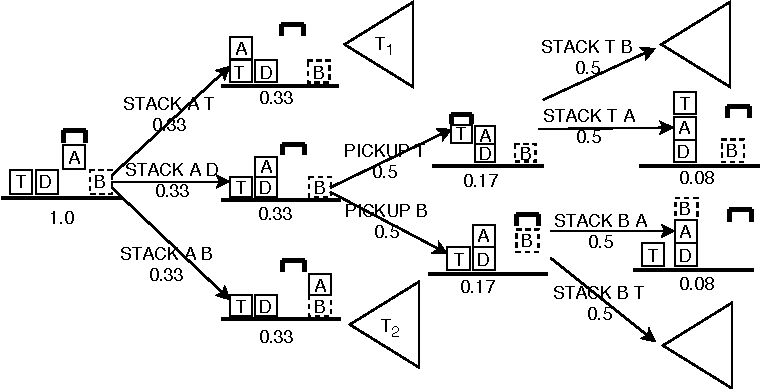
\includegraphics[width=0.8\textwidth]{img/featuresbw.pdf}}
        \caption{Fragment of the decision space after PICKUP A has been observed for block-words example in Figure \ref{fig:multi} (top). Numbers under each state and action indicate the probability. Sub trees $T_1$ and $T_2$ are not expanded for simplicity.}
        \label{fig:feature}
\end{figure*} 

\textbf{Risk ($R$)} quantifies the probability that the presented action will lead to $\mathrm{u}$. $R$ is also coupled with the uncertainty the observer has about what the next action the user or the competitor (if present) will present. We model the uncertainty as a uniform probability distribution across the set of actions whose preconditions are satisfied in current state. We define $R$ as the posterior probability of reaching $\mathrm{u}$ while the user is trying to achieve $\mathrm{d}$. We extract plans from the intervention graph from the root to any leaf containing the $\mathrm{d}$, including the plans in which the user has been subverted to reach $\mathrm{u}$ instead. By construction, $\mathrm{d}$ will always be a leaf.
Let $\Pi_{\mathcal{C}}$ be the candidate plans reaching $\mathrm{d}$ and let $\left | \Pi_{\mathcal{C}} \right |=n$. The plan set $\Pi_{u}$ contains action sequences that reach state $\mathrm{u}$ such that, $\Pi_{u} \subseteq \Pi_{\mathcal{C}}$, $\left | \Pi_{u} \right |=m$ and $(m<=n)$. We compute posterior probability of reaching $\mathrm{u}$ for a path $\pi \in \Pi_{u}$, using chain rule in probability as, $P_{\pi}=\prod_{j=1}^{k}P(\alpha_j|\alpha_1, \alpha_2,...,\alpha_{k-1})$, and $\alpha_{j} \in A$ and $k$ is the length of path until $\mathrm{u}$ is reached. Then: 
\begin{equation*} 
R = \left\{\begin{matrix} \frac{\sum_{i=1}^{m}P_{\pi_i}}{m} & m>0\\ 0 &  m=0 \end{matrix}\right.
\end{equation*}
In Figure \ref{fig:feature}, $(n=6)$ and $(m=1)$. Since we assumed full observability for the observer, the root of the tree (current state) is assigned the probability of 1.0. Actions that are immediately possible after the current state are each assigned probabilities following a uniform distribution across the branching factor (0.33). Then for each applicable action in the current state, the resulting state gets the probability of ($1.0\times0.33=0.33$). Similarly, we apply the chain rule of probability for each following state and action level in the graph until $\mathrm{u}$ first appears in the path. $R=\frac{0.08}{1}=0.08$.

\textbf{Desirability ($D$)} measures the effect of the observed action to help the user pursue the desirable goal safely. Given $\Pi_{\mathcal{C}}$ as the set of plans extracted from the intervention graph that reach $\mathrm{d}$ and $\left | \Pi_{\mathcal{C}} \right |=n$. The plan set $\Pi_{d}$ contains action sequences that reach state $\mathrm{d}$ without reaching $\mathrm{u}$, $\Pi_{d} = \Pi_{\mathcal{C}} \setminus \Pi_{u} $, we compute  posterior probability of reaching $\mathrm{d}$ without reaching $\mathrm{u}$ for a path $\pi \in \Pi_{d}$, using chain rule in probability as, $P_{\pi}=\prod_{j=1}^{k}P(\alpha_j|\alpha_1, \alpha_2,...,\alpha_{k-1})$, and $\alpha_{j} \in A$ and $k$ is the length of path. Then:
\begin{equation*} 
D = \left\{\begin{matrix}
\frac{\sum_{i=1}^{n-m}P_{\pi_i}}{n-m} & n-m>0\\ 
0 &  n-m=0
\end{matrix}\right.
\end{equation*} 
In Figure \ref{fig:feature}, there are five instances where user achieved $\mathrm{d}$  without reaching $\mathrm{u}$ (two in sub tree $T_1$, three in the expanded branch). Following the same approach to assign probabilities for states and actions, $D= \frac{(0.08+0.08+0.08+0.04+0.04)}{5} = 0.07$.
$R$ and $D$ are based on probabilities indicating the confidence the observer has about the next observation. We also use simple distance measures: (1) distance to $\mathrm{u}$  ($\delta_u$) and (2) distance to $\mathrm{d}$ ($\delta_d$). Both distances are measured in the number of actions required to reach a state containing $\mathrm{d}$ or $\mathrm{u}$ from root in the intervention graph.  

\textbf{Distance to $\boldsymbol{\mathrm{u}}$} ($\delta_u$) measures the distance to state $\mathrm{u}$ from the current state in terms of the number of actions. $\Pi_{\mathcal{C}}$ is the set of paths extracted from the intervention graph that reach $\mathrm{d}$ and $\left | \Pi_{\mathcal{C}} \right |=n$. The path set $\Pi_{u}$ contains action sequences that reach state $\mathrm{u}$ such that, $\Pi_{u} \subseteq \Pi_{\mathcal{C}}$, $\left | \Pi_{u} \right |=m$ and $(m<=n)$. We count  $s$, the number of the edges (actions) before $\mathrm{u}$ is reached for each path $\pi \in \Pi_{u}$ and $\delta_u$ is defined as the average of the distance values:
\begin{equation*} 
\delta_u = \left\{\begin{matrix}
\frac{\sum_{i=1}^{m}s_i}{m} & m>0\\ 
-1 &  m=0
\end{matrix}\right.
\end{equation*} 
In this formula, $-1$ indicates that the undesirable state is not reachable from the current state. For the example problem illustrated in Figure \ref{fig:feature}, $\delta_u=\frac{3}{1}=3$. 

\textbf{Distance to $\boldsymbol{\mathrm{d}}$} ($\delta_d$) measures the distance to $\mathrm{d}$ from current state. The path set $\Pi_{d}$ contains action sequences that reach $\mathrm{d}$ without reaching $\mathrm{u}$, $\Pi_{d} = \Pi_{\mathcal{C}} \setminus \Pi_{u} $, we count  $t$, the number of the edges where $\mathrm{d}$ is achieved without reaching $\mathrm{u}$ for each path $\pi \in \Pi_{d}$. Then, $\delta_d$ is defined as the average of the distances given by the formula:
\begin{equation*} 
\delta_d = \left\{\begin{matrix}
\frac{\sum_{i=1}^{n-m}t_i}{n-m} & n-m>0\\ 
-1 &  n-m=0
\end{matrix}\right.
\end{equation*}
In this formula, $-1$ indicates that $\mathrm{d}$ can not be reached safely from the current state. For the example problem illustrated in Figure \ref{fig:feature}, $\delta_d=\left \lceil \frac{3+3+7+7+3}{5} \right \rceil=5$.

\textbf{Percentage of active attack landmarks} ($\mathcal{L}_{ac}$) captures the criticality of the current state toward contributing to $\mathrm{u}$. 
Landmarks \cite{hoffman2004lm} are predicates (or actions) that must be true in every valid plan for a planning problem. We used the algorithm in Hoffmann et al. \shortcite{hoffman2004lm} to extract fact landmarks for the planning problem $P = \langle D, \mathrm{u}\rangle$. These landmarks are referred to as attack landmarks ($\mathcal{L}_{u}$) because they establish predicates that must be true to reach $\mathrm{u}$.  Landmarks have been successfully used in deriving heuristics in plan recognition \cite{vered2018goalrec} and generating alternative plans \cite{bryce2014diverse}. We compute the percentage of active attack landmarks in the current state ($\mathcal{L}_{ac}$). To compute $\mathcal{L}_{ac}$ in Figure \ref{fig:feature}, we count the number of landmark predicates that have become active $(l)$ in the root of the intervention graph. Then, ($\mathcal{L}_{ac}$) is given by the formula: $\mathcal{L}_{ac} = \frac{l}{\left |\mathcal{L}_{u}\right|}$. In Figure \ref{fig:feature}, $l=4$ and $\mathcal{L}_{ac}=4/10=0.4$.

For each presented action, the intervention graph is generated and features are computed, producing the corresponding feature vector for the presented action. Landmarks for the problem $P = \langle D, \mathrm{u}\rangle$ are computed apriori. 

\section*{Sampling the Intervention Graph}
To overcome the state space explosion in large domains, we propose a second method. Instead of finding plans from the full search space, the observer samples only a subset of plans to compute a new feature vector called Sampled Features. Here, we estimate the Risk and Desirability using plan distance measures. If the user is executing an unsafe plan, then that plan should be more similar to a sample of unsafe plans, compared to a sample of safe plans. 

The observer computes plan distances between a reference plan ($\pi^\prime$) and sampled plans ($\Pi^{\prime\prime}$) for both $\mathrm{u}$ and $\mathrm{d}$ for each presented action. 
We follow the method proposed by Vered et al. \shortcite{vered2017} to generate the observation compatible plan by concatenating the observation history with the optimal plan that reaches $\mathrm{u}$ (and $\mathrm{d}$) to produce $\pi^\prime$. 

 We use the Top-K planner with K$=$50 \cite{riabov2014}, to sample the plan space.
We use action set distance (ASD), state sequence distance (SSD), causal link distance (CLD) \cite{nguyen2012generating}, Generalized Edit Similarity (GED) for sequences of states and actions \cite{sohrabi2016finding} as to measure the distance. When an action is presented to the observer, $\pi^\prime$ is computed. Then, observation compatible Top-K plans are produced for $\mathrm{u}$ and $\mathrm{d}$ separately. Then we compute the medians of ACD, CLD and SSD, minimum remaining actions to $\mathrm{u}$ and $\mathrm{d}$, minimum action GED and state GED are computed for $\mathrm{u}$ and $\mathrm{d}$ for all $\langle$reference, sample$\rangle$ pairs. This produces the Sampled Feature vector for the presented action.
%
%
%%\vspace{-2mm}
%%\begin{algorithm}[tb]
%%%\scriptsize
%%        \caption{Build Full Vectors}
%%        \label{alg:exact}
%%        \begin{algorithmic}[1]
%%                \Require $D$, $I$, $O$, $\mathrm{u}$, $\mathrm{d}$.
%%                \Procedure{Full}{$D,O,I,\mathrm{u},\mathrm{d}$}
%%                \State $i=0;$ $ s_i \gets I$
%%                \State $\mathcal{L}_{u} \gets$ compute remaining landmarks for the problem $P_\alpha=\langle D_\alpha, \mathrm{u}\rangle$
%%                \For{$o \in O$}
%%                        \State $G(V,E) \gets ExpandGraph(D,s_i,\mathrm{u},\mathrm{d})$
%%                        \State $R_o \gets$ compute $Risk$ using $IG$
%%                        \State $D_o \gets$ compute $Desirability$ using $IG$
%%                        \State $\delta_{u_o} \gets$ compute mean distance to critical state using $IG$
%%                        \State $\delta_{d_o} \gets$ compute mean distance to desirable state using $IG$
%%                        \State $\mathcal{L}_{{ac}_o} \gets$ active landmark \% using $s_i$ and  $\mathcal{L}_{u}$
%%                        \State $\mathcal{V}(o) \gets \lbrack R_o,D_o,\delta_{u_o}, \delta_{d_o}, \mathcal{L}_{{ac}_o}\rbrack$
%%                        \State {$s_{i+1} \gets ((s_{i} \setminus Del(o))\cup Add(o))$}
%%                \EndFor
%%                \EndProcedure
%%        \end{algorithmic}
%%\end{algorithm}
%%\setlength{\textfloatsep}{2pt}
%%\begin{algorithm}[tb]
%%%\scriptsize
%%        \caption{Build Sampled Vector}
%%        \label{alg:apx}
%%        \begin{algorithmic}[1]
%%                \Require $D$, $s$, $\mathrm{u}$, $\mathrm{d}$
%%                \State $i=0;$ $ s_{i} \gets I $
%%                \State $prefix,suffix,\Pi^{\prime\prime}, \mathcal{V} \gets \varnothing$
%%                \Procedure{Partial}{$D,s,\mathrm{u},\mathrm{d},O$}
%%                        \State $\mathcal{L}_{u} \gets$ compute remaining landmarks for the problem $P_\alpha=\langle D_\alpha, \mathrm{u}\rangle$
%%                \For{$o \in O$}
%%                        \State \parbox[t]{0.95\linewidth}{$prefix \gets prefix + o$}
%%                        \State \parbox[t]{0.95\linewidth} 
%%                                {$s_{i+1} \gets ((s_{i} \setminus Del(o))\cup Add(o))$}
%%                        \For {$ g \in \{\mathrm{u}, \mathrm{d}$\}}
%%                                \State \parbox[t]{0.95\linewidth}{$suffix \gets OptimalPlan(s,g)$}
%%                                \State \parbox[t]{0.95\linewidth}{$\Pi^\prime \gets prefix + suffix$}
%%                                \State \parbox[t]{0.95\linewidth}{$\Pi^{\prime\prime} \gets \text{Observation compatible Top-K plans for } g$}
%%                                \State \parbox[t]{0.95\linewidth}{$v_1 \gets$ MedianActionSetDist$(\Pi^\prime, \Pi^{\prime\prime})$}
%%                                \State \parbox[t]{0.95\linewidth}{$v_2 \gets$ MedianCausalLinkDist$(\Pi^\prime, \Pi^{\prime\prime})$}
%%                                \State \parbox[t]{0.95\linewidth}{$v_3 \gets$ MedianStateSequenceDist$(\Pi^\prime,\Pi^{\prime\prime})$}
%%                                \State \parbox[t]{0.95\linewidth}{$v_4 \gets$ MinimumDistToState $(g,\Pi^{\prime\prime})$}
%%                                \State \parbox[t]{0.95\linewidth}{$v_5 \gets$ MinimumActionGED $(\Pi^\prime, \Pi^{\prime\prime})$}
%%                                \State \parbox[t]{0.95\linewidth}{$v_6 \gets$ MinimumStateGED $(\Pi^\prime, \Pi^{\prime\prime})$}
%%                                \State $\mathcal{V}(o) \gets \lbrack v_1,v_2,v_3,v_4,v_5,v_6\rbrack $
%%                        \EndFor
%%                        \State \parbox[t]{0.95\linewidth}{$v_7 \gets$ AchievedLandmarkHeuristic $(\mathrm{u},s_{i})$}
%%                        \State $\mathcal{V}(o) \gets \mathcal{V}(o)+\{v_7\}$
%%                \EndFor
%%                \EndProcedure
%%        \end{algorithmic}
%%\end{algorithm}
%
%%=========================================================================
%%=========================================================================
%%=== algorithm
%%=========================================================================
%%=========================================================================
\section*{Learning When to Intervene}
We train a classifier to categorize the presented action into two classes: (Y) indicating intervention is required and (N), indicating otherwise. Given observations labeled as Y/N and corresponding feature vectors, we train the classifiers with 10-fold cross validation. The trained model is used to predict intervention for previously unseen intervention problems. We chose Naive Bayes, K-nearest neighbors, decision tree and logistic regression classifiers from Weka~\footnote{\url{http://www.cs.waikato.ac.nz/ml/weka/}}. Attribute selected classifiers filter the feature vector to only select critical features. This step reduces complexity of the model, makes the outcome of the model easier to interpret, and reduces over-fitting.
% We selected these classifiers because they are commonly used interpretable models, which we hope to utilize in generating explanations for intervention in future work.

We generated training data from twenty intervention problems using the benchmark domains. Additionally, we created a new planning domain for the Rush Hour puzzle. In this puzzle, user moves vehicle objects on a grid to clear a path for a target vehicle to move to the exit located on the perimeter of the grid. We created training data from twenty Rush Hour puzzles. We restricted the number of observation traces per intervention problem to 100.
 
A full parameter search revealed the best parameters for the classifiers. The decision tree classifier is tuned to pruning confidence=0.25 and minimum number of instance per leaf=2. K-nearest neighbor classifier is tuned to use k=1 and distance measure=Euclidean. The logistic regression classifier is tuned for ridge parameter = 1.0E-8. Naive Bayes classifier is tuned with the supervised discretization=True. For the intervention graph approach, the learned models chose distance to $\mathrm{u}$ and Risk as the dominant features for the benchmark domains. 
%We were not able to identify clear dominant features in feature vectors built with plan space sampling.

We ran experiments using the Weka workbench to evaluate classifier accuracy (dependent variable) to varying parameter for the classifiers (independent variables). Table \ref{tab:tuned} summarizes results, with boldface values indicating the selected parameter values that produced best accuracy (95\% confidence interval) for all the domains.
\begin{table}[ht]
\small
\begin{tabular}{|l|l|}
\hline
\multicolumn{1}{|c|}{Classifier} & \multicolumn{1}{c|}{Tested Values}                                                        \\ \hline
Decision tree                    & \begin{tabular}[c]{@{}l@{}}C = {[}0.05,0.1,\textbf{0.25},0.5{]}\\ M = {[}\textbf{2},5,10{]}\end{tabular}    \\ \hline
K-nearest neighbor               & \begin{tabular}[c]{@{}l@{}}K = {[}\textbf{1},3,7{]}\\ Dis = {[}\textbf{Eucledean},Manhattan{]}\end{tabular} \\ \hline
Naive Bayes                      & D = {[}\textbf{True},False{]}                                                                      \\ \hline
Logistic regression              & R = {[}1.0E-2,1.0E-4,\textbf{1.0E-8},1.0E-16{]}                                                    \\ \hline
\end{tabular}
\caption{Parameter tuning for intervention classifiers}
\label{tab:tuned}
\end{table}
%% 
% 
%%=========================================================================
%%=========================================================================
%%=== results
%%=========================================================================
%%=========================================================================
\section*{Results and Discussion}
We focus on two questions: (1) Using domain-independent features indicative of the likelihood to reach $\mathrm{u}$ from current state, can the observer correctly interrupt to prevent the user from reaching $\mathrm{u}$? and (2) How does the learning approach perform against state-of the-art goal recognition? To address the first question, we evaluated the performance of the learned model on unseen problems.

The benchmark suite consists of Blocks-words, IPC Grid, Navigator and Ferry domains and the Generalized Rush Hour domain. For the \textbf{Blocks-words} domain, we chose word building problems. The words the user and the competitor want to build are different but they have some common letters. In the \textbf{IPC grid} domain, the user agent moves through a grid to get from point A to B. Certain locked positions on the grid can be opened by picking up keys. In the \textbf{Navigator} domain, the user agent moves from one point in grid to another. In IPC Grid and Navigator domains, we designated certain locations on the grid as traps. The goal of the user is to navigate to a specific point on the grid without passing through the trap. In the \textbf{Ferry} domain, a single ferry moves cars between different locations. We assigned a port as \emph{compromised}. The ferry's objective is to transport cars to specified locations without passing the compromised port. In the \textbf{Rush Hour} domain, we created puzzles on arbitrary grid sizes and exits. The player wins by moving a target car to the exit. We also designated some vehicles on the grid as forbidden. The forbidden vehicles need not be moved to solve the puzzle. Any user action that moves any of the forbidden vehicles raises the intervention flag.

We generate 3 separate test instances of 20 problems each (total of 60) for the benchmark domains with problems different from training instances. For example, number of blocks in the blocks words domain, size of grid (navigator, IPC-Grid), number of cars and exit locations  in Rush Hour domain, accessible and inaccessible paths on the grid (navigator, IPC-Grid), properties of artifacts in the grid (IPC-Grid). For each problem in test instance we generated 10 observation traces (total of 600 test observation traces). For the Rush Hour domain we created 2200 observation traces and split to training and testing 60/40. We define true-positive as the classifier correctly identifying the presented action as action that must be in $a_{crit}$ or $q_{crit}$. True-negative is an instance where the classifier  correctly identifying an action as not belonging to $a_{crit}$ or $q_{crit}$. False-positives are instances where classifier incorrectly identifies an action as belonging to $a_{crit}$ or $q_{crit}$. False-negatives are instances where the classifier incorrectly identifies the presented action as not belonging to $a_{crit}$ or $q_{crit}$. Naturally, our test observation traces contain a large number of negatives. To offset the bias introduced to the classifier by the class imbalance, we report Matthews correlation coefficient (MCC) because it gives an accurate measure the quality of a binary classification while taking into account the different class sizes. We also report the F-score $= \frac{tp}{tp+1/2(fp+fn)}$ for the classifiers. $tp$, $fp$, $fn$ are the number of true positives, false positives and false negatives respectively.


\begin{table*}[tb]
\resizebox{\textwidth}{!}{%
\begin{tabular}{|l|llllll|llllll|llllll|llllll|}
\hline
\multicolumn{1}{|c|}{\multirow{3}{*}{Domain}} & \multicolumn{6}{c|}{Naive Bayes}                                                                                                          & \multicolumn{6}{c|}{Decision Tree}                                                                                                      & \multicolumn{6}{c|}{Logistic Regression}                                                                                                & \multicolumn{6}{c|}{K-Nearest}                                                                                                             \\ \cline{2-25} 
\multicolumn{1}{|c|}{}                        & \multicolumn{2}{c|}{Inst 1}                        & \multicolumn{2}{c|}{Inst 2}                        & \multicolumn{2}{c|}{Inst 3}     & \multicolumn{2}{c|}{Inst 1}                        & \multicolumn{2}{c|}{Inst 2}                        & \multicolumn{2}{c|}{Inst 3}   & \multicolumn{2}{c|}{Inst 1}                        & \multicolumn{2}{c|}{Inst 2}                        & \multicolumn{2}{c|}{Inst 3}   & \multicolumn{2}{c|}{Inst 1}                         & \multicolumn{2}{c|}{Inst 2}                         & \multicolumn{2}{c|}{Inst 3}    \\ \cline{2-25} 
\multicolumn{1}{|c|}{}                        & \multicolumn{1}{l|}{F-score} & \multicolumn{1}{c|}{MCC} & \multicolumn{1}{c|}{F-score} & \multicolumn{1}{l|}{MCC} & \multicolumn{1}{l|}{F-score} & MCC   & \multicolumn{1}{l|}{F-score} & \multicolumn{1}{l|}{MCC} & \multicolumn{1}{l|}{F-score} & \multicolumn{1}{l|}{MCC} & \multicolumn{1}{l|}{F-score} & MCC & \multicolumn{1}{l|}{F-score} & \multicolumn{1}{l|}{MCC} & \multicolumn{1}{l|}{F-score} & \multicolumn{1}{l|}{MCC} & \multicolumn{1}{l|}{F-score} & MCC & \multicolumn{1}{l|}{F-score} & \multicolumn{1}{l|}{MCC}  & \multicolumn{1}{l|}{F-score} & \multicolumn{1}{l|}{MCC}  & \multicolumn{1}{l|}{F-score} & MCC  \\ \hline
\multicolumn{25}{|c|}{Intervention Graph Method}                                                                                                                                                                                                                                                                                                                                                                                                                                                                                                                                                                                         \\ \hline
\textbf{Blocks}              & 1                       & \multicolumn{1}{l|}{1}   & 1                       & \multicolumn{1}{l|}{1}   & 1                       & 1     & 1                       & \multicolumn{1}{l|}{1}   & 1                       & \multicolumn{1}{l|}{1}   & 1                       & 1   & 1                       & \multicolumn{1}{l|}{1}   & 1                       & \multicolumn{1}{l|}{1}   & 1                       & 1   & 1                       & \multicolumn{1}{l|}{1}    & 1                       & \multicolumn{1}{l|}{1}    & 1                       & 1    \\ \cline{1-1}
\textbf{EasyIPC}             & 1                       & \multicolumn{1}{l|}{1}   & 1                       & \multicolumn{1}{l|}{1}   & 1                       & 1     & 1                       & \multicolumn{1}{l|}{1}   & 1                       & \multicolumn{1}{l|}{1}   & 1                       & 1   & .88                     & \multicolumn{1}{l|}{.87} & .88                     & \multicolumn{1}{l|}{.87} & .86                     & .86 & 1                       & \multicolumn{1}{l|}{1}    & 1                       & \multicolumn{1}{l|}{1}    & 1                       & 1    \\ \cline{1-1}
\textbf{Ferry}               & 1                       & \multicolumn{1}{l|}{1}   & 1                       & \multicolumn{1}{l|}{1}   & 1                       & 1     & 1                       & \multicolumn{1}{l|}{1}   & 1                       & \multicolumn{1}{l|}{1}   & 1                       & 1   & 1                       & \multicolumn{1}{l|}{1}   & 1                       & \multicolumn{1}{l|}{1}   & 1                       & 1   & 1                       & \multicolumn{1}{l|}{1}    & 1                       & \multicolumn{1}{l|}{1}    & 1                       & 1    \\ \cline{1-1}
\textbf{Navigator}           & 1                       & \multicolumn{1}{l|}{1}   & 1                       & \multicolumn{1}{l|}{1}   & .99                     & .99   & .87                     & \multicolumn{1}{l|}{.87} & .72                     & \multicolumn{1}{l|}{.74} & .90                     & .90 & 1                       & \multicolumn{1}{l|}{1}   & 1                       & \multicolumn{1}{l|}{1}   & .99                     & .99 & 1                       & \multicolumn{1}{l|}{1}    & .96                     & \multicolumn{1}{l|}{.96}  & .99                     & .99  \\ \hline
\multicolumn{25}{|c|}{Plan Space Sampling Method}                                                                                                                                                                                                                                                                                                                                                                                                                                                                                                                                                                                      \\ \hline
\textbf{Blocks}              & .25                     & \multicolumn{1}{l|}{.33} & .25                     & \multicolumn{1}{l|}{.33} & .25                     & .33   & .25                     & \multicolumn{1}{l|}{.33} & .25                     & \multicolumn{1}{l|}{.33} & .25                     & .33 & .25                     & \multicolumn{1}{l|}{.33} & .25                     & \multicolumn{1}{l|}{.33} & .25                     & .33 & 1                       & \multicolumn{1}{l|}{1}    & 1                       & \multicolumn{1}{l|}{1}    & 1                       & 1    \\ \cline{1-1}
\textbf{EasyIPC}             & 1                       & \multicolumn{1}{l|}{1}   & 1                       & \multicolumn{1}{l|}{1}   & 1                       & 1     & 1                       & \multicolumn{1}{l|}{1}   & 1                       & \multicolumn{1}{l|}{1}   & 1                       & 1   & .64                     & \multicolumn{1}{l|}{.63} & .46                     & \multicolumn{1}{l|}{.44} & .67                     & .66 & .05                     & \multicolumn{1}{l|}{-.04} & .04                     & \multicolumn{1}{l|}{-.03} & .05                     & -.02 \\ \cline{1-1}
\textbf{Ferry}               & .34                     & \multicolumn{1}{l|}{.33} & .32                     & \multicolumn{1}{l|}{.31} & 0.02                    & -.004 & .25                     & \multicolumn{1}{l|}{.28} & .24                     & \multicolumn{1}{l|}{.23} & .86                     & .86 & .31                     & \multicolumn{1}{l|}{.32} & .23                     & \multicolumn{1}{l|}{.22} & 1                       & 1   & .33                     & \multicolumn{1}{l|}{.40}  & .13                     & \multicolumn{1}{l|}{.15}  & .81                     & .82  \\ \cline{1-1}
\textbf{Navigator}           & 1                       & \multicolumn{1}{l|}{1}   & 1                       & \multicolumn{1}{l|}{1}   & 1                       & 1     & .62                     & \multicolumn{1}{l|}{.65} & 1                       & \multicolumn{1}{l|}{1}   & 1                       & 1   & .60                     & \multicolumn{1}{l|}{.59} & .98                     & \multicolumn{1}{l|}{.94} & .97                     & .97 & .61                     & \multicolumn{1}{l|}{.65}  & 1                       & \multicolumn{1}{l|}{1}    & 1                       & 1    \\ \cline{1-1}
\textbf{Rush Hour}           & .44                     & .40                      &                         &                          &                         &       & .89                     & .89                      &                         &                          &                         &     & .56                     & .54                      &                         &                          &                         &     & .89                     & .89                       &                         &                           &                         &      \\ \hline
\end{tabular}%
}
\caption{F-score and MCC for predicting intervention using  Intervention Graph and plan space sampling methods}
\label{tab:exactapprox}
\end{table*}




\begin{table}[tb]
\resizebox{\textwidth}{!}{%
\begin{tabular}{|l|ll|ll|ll|ll|ll|ll|ll|ll|ll|}
\hline
\multicolumn{1}{|c|}{\multirow{3}{*}{Domain}} & \multicolumn{6}{c|}{Inst 1}                                                                                        & \multicolumn{6}{c|}{Inst 2}                                                                    & \multicolumn{6}{c|}{Inst 3}                                                                    \\ \cline{2-19} 
\multicolumn{1}{|c|}{} & \multicolumn{2}{l|}{RG (LAMA)}  & \multicolumn{2}{l|}{RG (HSP)} & \multicolumn{2}{c|}{GM}       & \multicolumn{2}{c|}{RG (LAMA)} & \multicolumn{2}{c|}{RG (HSP)} & \multicolumn{2}{c|}{GM}       & \multicolumn{2}{c|}{RG (LAMA)} & \multicolumn{2}{c|}{RG (HSP)} & \multicolumn{2}{c|}{GM}       \\ \cline{2-19} 
\multicolumn{1}{|c|}{}                        & \multicolumn{1}{c|}{F-score} & \multicolumn{1}{c|}{MCC} & \multicolumn{1}{l|}{F-score} & MCC & \multicolumn{1}{l|}{F-score} & MCC & \multicolumn{1}{l|}{F-score}  & MCC & \multicolumn{1}{l|}{F-score} & MCC & \multicolumn{1}{l|}{F-score} & MCC & \multicolumn{1}{l|}{F-score}  & MCC & \multicolumn{1}{l|}{F-score} & MCC & \multicolumn{1}{l|}{F-score} & MCC \\ \hline
\textbf{Blocks}  & .38    & .45  & .38   & .45 & .36  & .43 & .43  & .49 & .43                     & .49 & .39  & .45 & .40  & .47 & .40  & .47 & .38  & .45 \\ \cline{1-1}
\textbf{EasyIPC}                              & .13                     & .05                      & .13                     & .05 & .10                     & .01 & .21                      & .17 & .18                     & .13 & .12                     & .06 & .23                      & .19 & .22                     & .19 & .14                     & .09 \\ \cline{1-1}
\textbf{Ferry} & .17  & .18                      &.22                         & .20    & .10                     & .08 & .22                      & .23 &      .11                   &   .06  & .15                     & .09 & .15                      & .17 &              .47           &   .52  & .21                     & .34 \\ \cline{1-1}
\textbf{Navigator}                            & -                       & -                        & -                       & -   & -                       & -   & -                        & -   & -                       & -   & -                       & -   & -                        & -   & -                       & -   & -                       & -   \\ \hline
\end{tabular}%
}
\caption{F-score and Maththews Correlation Coefficient (MCC) for recognizing intervention with probabilistic goal recognition (RG) using a satisficing (LAMA) and optimal (HSP) planners and goal mirroring(GM). For the Navigator domain intervention problems, the true-negative, false negative rates were 100\%  each. Therefore, F-score and MCC are not reported for that problem set.}
\label{tab:rgv}
\end{table}

We implemented three state-of-the art plan recognition algorithms to compare intervention accuracy to the proposed learning based solution. We selected Ramirez and Geffener's probabilistic plan recognition algorithm \cite{ramirez2010probabilistic} (both the satisficing, and optimal implementations) and the Goal Recognition with Goal Mirroring algorithm by Vered et al. \shortcite{vered2018goalrec}. 
For each presented action, the observer solves a plan recognition problem using each approach. We assumed uniform priors for over $\mathrm{u}$ and $\mathrm{d}$. If $\mathrm{u}$ is the top ranked goal for the presented action, then it is flagged as requiring intervention. The assumption is that these algorithms must also be able to correctly identify $\mathrm{u}$ as most likely goal for the actions in $a_{crit}$ and $q_{crit}$. We used the same test data suite to evaluate accuracy.

Table \ref{tab:exactapprox} shows that the classifiers trained with features from the intervention graph achieve high accuracy for all the domains when predicting intervention. The MCC value shows that the class size does not bias the classifier. Low false positives and false negatives suggests that the user will not be unnecessarily interrupted. As expected performance degrades when we use a sampled plan space to derive features. For the benchmark domains we were able to discover at least one classifier responded with very high F-score the plan similarity features, the exception being the Ferry domain. The Rush Hour domain produced comparatively better results, with the decision tree and K-Nearest neighbor classifiers being the best. 

Features derived from the intervention graph accurately separate actions where the user has limited options available to reach the desirable goal while avoiding the undesirable state. Thus the classifiers perform well in recognizing critical actions in new problems. The sampled features rely on the learning algorithm to produce better output when predicting intervention. 

Comparing results in Table \ref{tab:rgv}, learning methods outperform existing plan recognition algorithms when predicting intervention. The algorithms we selected clearly struggled to predict intervention in the Navigator domain. 
These results suggest that although we can adopt existing plan recognition algorithms to identify when the user needs intervention, it also produces a lot of false negatives and false positives in correctly identifying which state (desirable/undesirable) is most likely given the observations. The learning approach is better suited for intervention because the observer can target specific critical actions and allow the user some freedom.

\section*{Conclusion}
When agents work in environments with hidden information, their plans can go wrong.
We formalized the online plan intervention problem to recognize when plans will not achieve the intended goal. We proposed two learned models that use features extracted from the intervention graph and the sampled plan space to identify critical actions and critical sequences, which if not intervened will cause the user agent's plan to fail. We evaluated how existing classifiers perform in predicting intervention. The learning approach outperforms existing online plan recognition approaches in predicting intervention with lower false positives and false negatives.



%%%%%%%%%%%%%%%%%%%%%%%%%%%%%%%%%%%%%%%%%%%%%%%%%%%%%%%%%%%%%%%%
\chapter{Research In-Progress: Studying Human User Behavior In-Situ}

%%%%%%%%%%%%%%%%%%%%%%%%%%%%%%%%%%%%%%%%%%%%%%%%%%%%%%%%%%%%%%%%

This chapter briefly describes the human subject experiments on the two new planning domains: cyber-security and Rush Hour puzzle. We have completed the cyber-security human subject experiment. The Rush Hour experiment is now in progress.

\section*{Home Computer User Behavior in Questionable Security Scenarios}
Home computer use, as distinguished from work related or organizationally based computer use, is dominated by personal activities (mostly recreational, but some financial and health related) and is not governed by security policies determined by experts. Our experiment protocol contained these common home computer user behaviors.

The primary goals of the experiment is to:
\begin{itemize}
 \item Capture actions taken by users when asked to perform tasks that provided ``opportunities'' to trigger security vulnerabilities
 \item Characterizing their behaviors by their gender and prior experience
 \item Assessing consistency in subject's survey answers and actual behavior.
 \end{itemize}

Many studies on assessing human decision making in practicing computer security  report that one major challenge in conducting security user studies is the disparities between self-reported and actual observations. Questions asked in self-reporting surveys induces respondent bias. For example in Ng et al. study \cite{ng2007}, the user is asked the question ``\textit{I am confident of recognizing suspicious email headers. (agree/disagree)}'' to measure self-efficacy. Users may find it difficult to estimate there skill level for some task and often times overestimate. Furthermore, asking about computer security practices primes the user for security, which may be difficult for researchers to control. A human subject study that looked into effectiveness of SSL (Securre Socket Layer) warnings that appear during Web browsing tasks \cite{sotirakopoulos2011} attempts to minimize the priming effect by designing tasks for the Web browsers the participants normally used and simulating the same look and feel of the native Web browsers. This study also used deception. The researchers did not reveal the true purpose of the study until the tasks were completed. The results of this study also confirms that there is a disparity between self-reported  and observed actions in computer security studies. We follow the same principles in our sandbox environment design and the administering the experiment. The sandbox environment has the same look and feel as the typical Microsoft Windows Desktop. We adopted deception by presenting the participants with a cover story, which stated that we were evaluating the participants on their ability to perform day-to-day computing tasks like checking email and web browsing. We also use a combination of surveys and observational data to identify predictors of user actions. Surveys are issued to participants at the beginning and at the end of the study to more accurately gauge what the users report and what they had actually done.


Another challenge in human subject studies in computer security practices is the sample bias. Characteristics of the study participants vary from the general population of computer users.  Many studies use university students as the subject pool \cite{sotirakopoulos2011, warkentin2016} in order to draw a representative sample to the best of their ability. However, typical computer users are young, old, tech-savvy, non-tech-savvy, educated, uneducated, male, female and so on. The diversity of the sample should lead to more generalizable data. In our study, we also use the university students as a sample mainly because it is a sample of convenience. We however restricted the student sample to consist of non computer science majors so that we can better approximate an average home computer user.

\subsection*{The Sandbox Environment}
The sandbox environment offers the subject a simulated desktop environment, which includes common applications such as emailing, Web-browsing, social networking, etc. As the subject performs these activities, different events happen that can trigger threats and vulnerabilities of interest to the researcher. These events may include asking the user to register with a login name and a password, to provide sensitive information to gain access to a site, to respond to pop-ups asking the user to download a software, etc. The system records the user responses to these actions, including user clicks and time taken for response.

Microsoft Windows is one of the most widely used desktop computing platforms accounting for 88\% of the market \cite{zdnet2020}. Thus, the look-and-feel of the Windows desktop and common applications is important to instilling familiarity for subjects. When a subject starts, he/she sees a Desktop as shown in Figure \ref{fig:desktop}. The Desktop provides application icons, e.g., a web-browser and a file-browser. Subjects can click these icons to launch the corresponding applications.

\begin{figure}[!ht]
  \centering
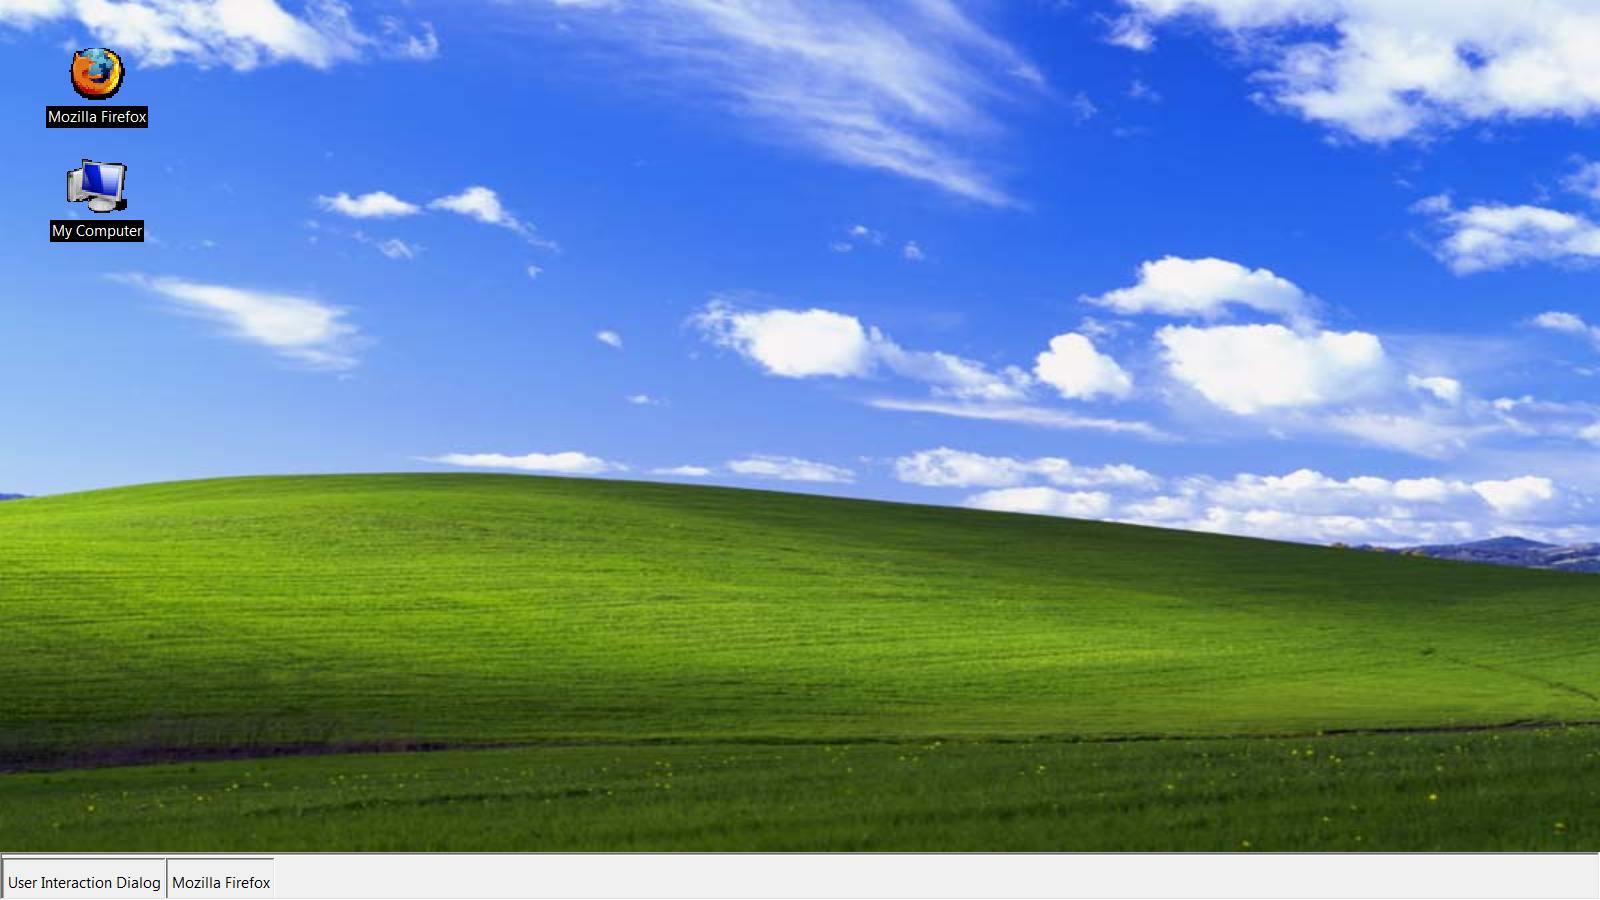
\includegraphics[width=\columnwidth]{img/desktop.png}
  \caption{Simulated Microsoft Windows desktop environment}
  \label{fig:desktop}
\end{figure}

Studies on global Internet users show that checking email, sending/receiving direct messages, browsing for information/research and social media activities account for the bulk of the online activities \cite{furnell2007, worldinternet2018}. Thus, simulating these activities was a priority for our sandbox environment; the current version includes simulated applications of email and Twitter. We used the open source Mozilla Firefox web browser for the Internet related tasks. We used SquirrellMail (version 1.4.22) as our email application. The subjects can look at a list of messages, read and answer them. For purposes of this study, the email accounts were populated with a set of email messages that were related to the other applications in the experiment protocol.

\begin{figure}[!ht]
  \centering
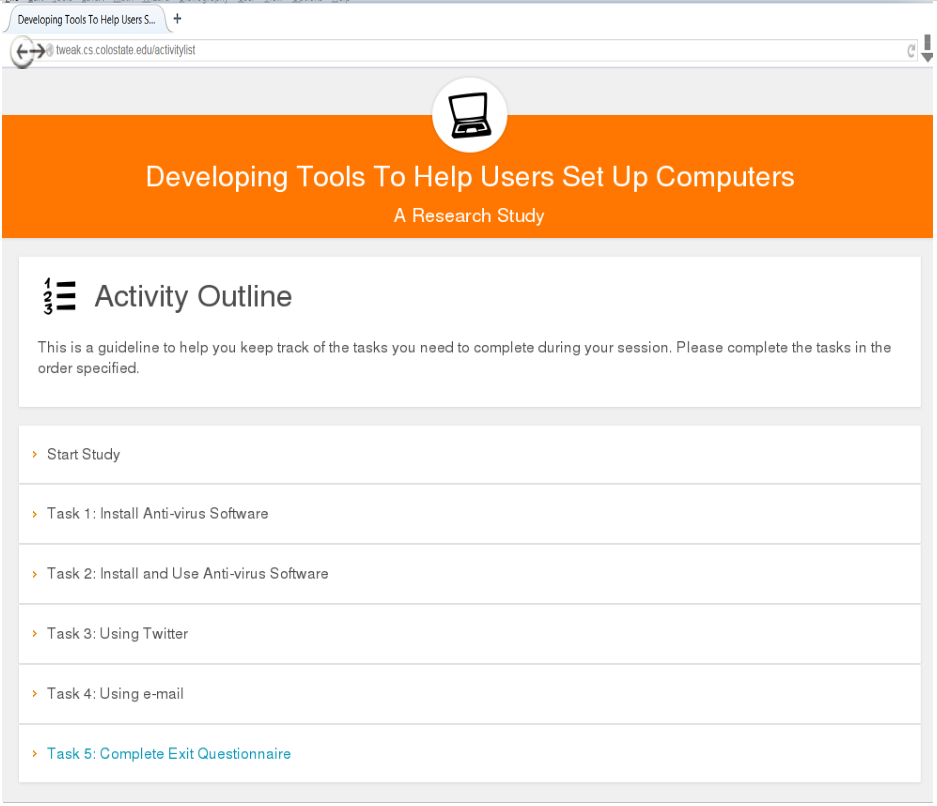
\includegraphics[width=\columnwidth, keepaspectratio=true]{img/browser.png}
  \caption{Simulated Mozilla Firefox Web browser}
  \label{fig:browser}
\end{figure}

As with email, our Twitter application supports login and message functions. Each participating user was provided with a twitter handle and a password. Three messages were posted in their respective Twitter inboxes (see Figure \ref{fig:twithome}). One of the three messages as shown in Figure \ref{fig:twitmsg}, which appears to link to a phishing website; if they click on the link, they are taken to a site which requested subjects to provide their Twitter username and password. 
\begin{figure}[ht]
  \centering
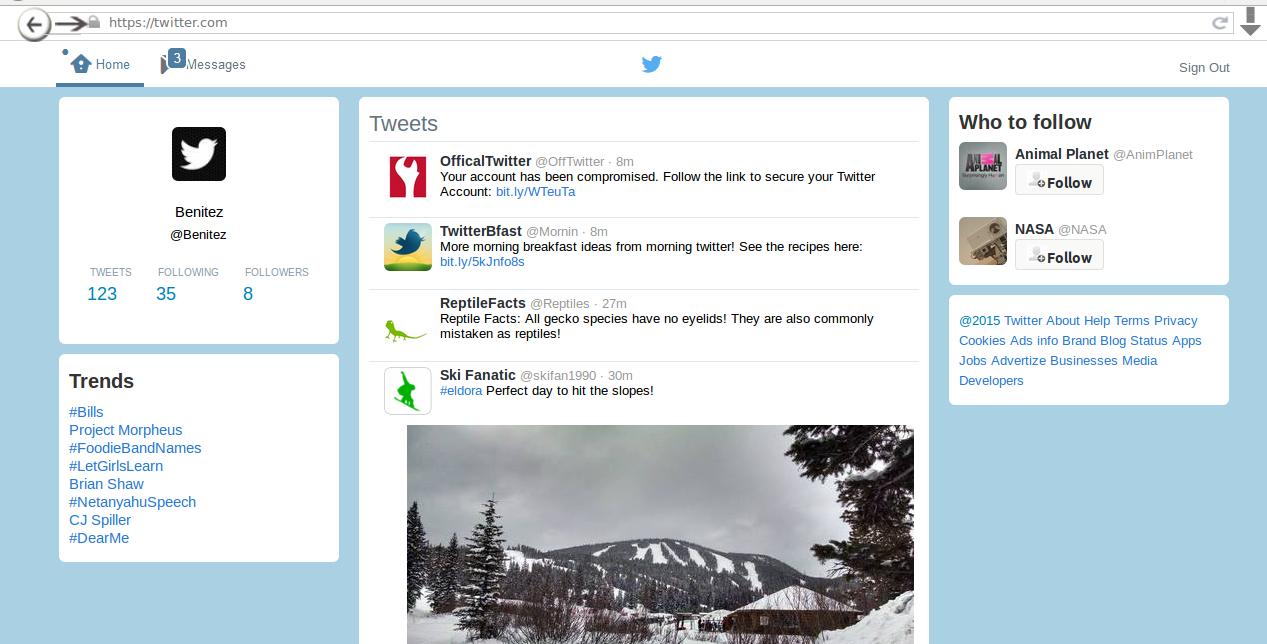
\includegraphics[width=\columnwidth, keepaspectratio=true]{img/twitterhome.png}
  \caption{Simulated Twitter home page with three direct messages in the inbox}
  \label{fig:twithome}
\end{figure}

\begin{figure}[ht]
  \centering
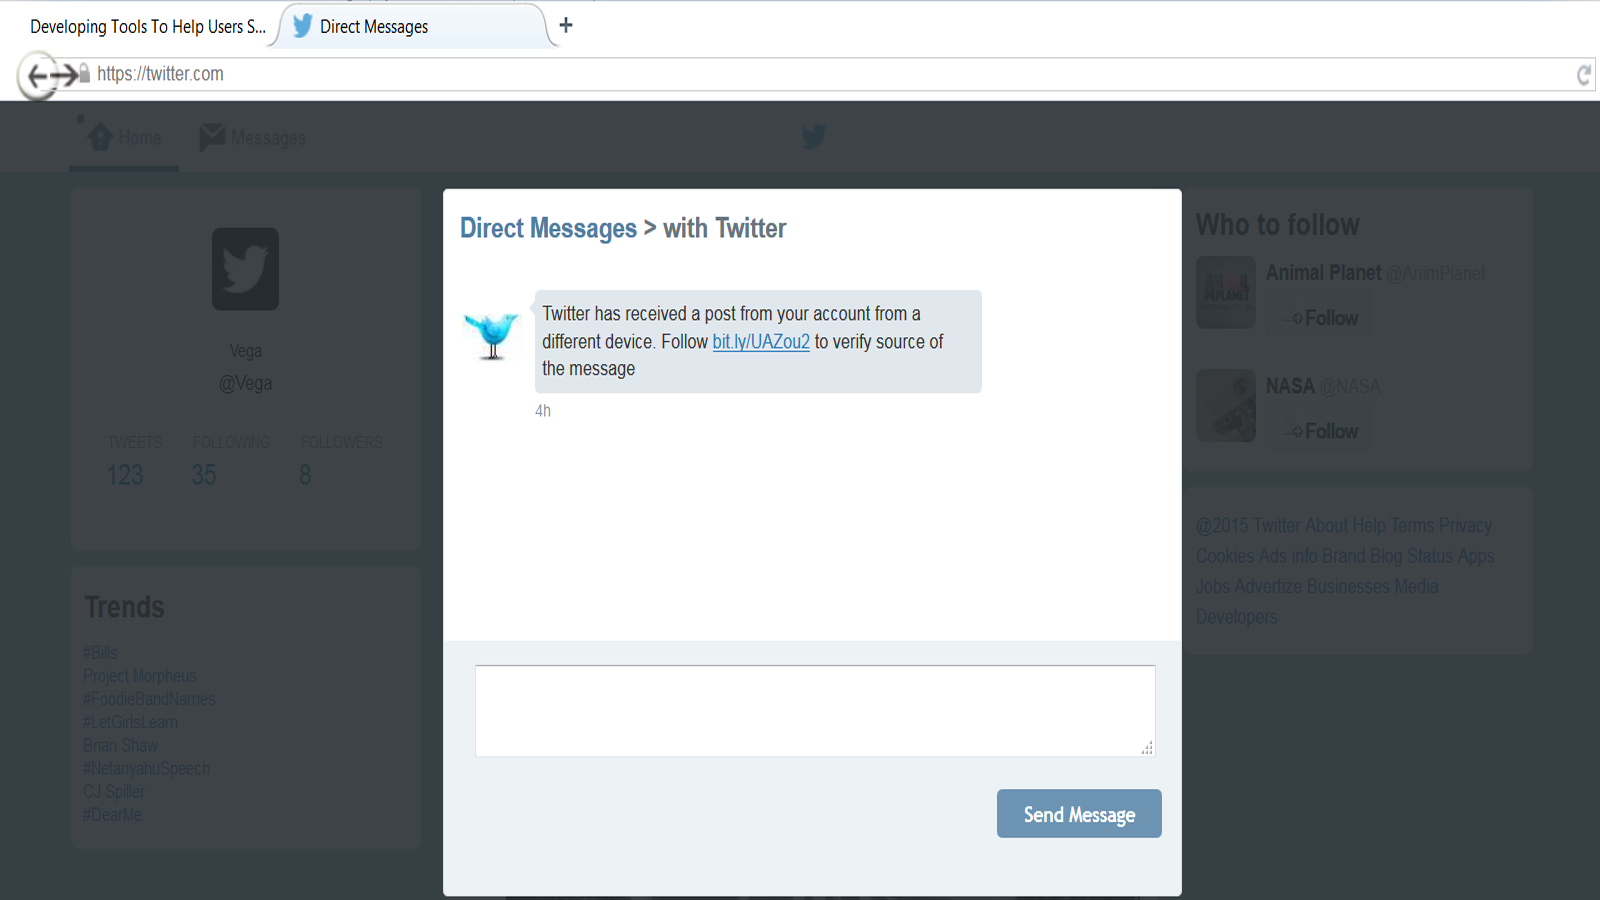
\includegraphics[width=\columnwidth, keepaspectratio=true]{img/twitter.png}
  \caption{Simulated Twitter direct message}
  \label{fig:twitmsg}
\end{figure}

As another activity, we included anti-virus software selection and installation. The subjects accessed an anti-virus download portal which leads to two separate websites as shown in Figure \ref{fig:virus}. One of the web-sites was purposefully made secure (HTTPS) while the other was made to look like a typical phishing site with flash images and dramatic warnings. Once the applications were downloaded, the subject was notified of the completed download. The subjects were then required to install and/or run the applications. To make sure the subjects installed and ran the downloaded application, the portal requested a verification code which was obtained by running the downloaded applications. Both anti-virus `downloads' were equipped with simulated system scanning capabilities (e.g., a progress bar appearing after the system scan is started).
\begin{figure}[htb]
  \centering
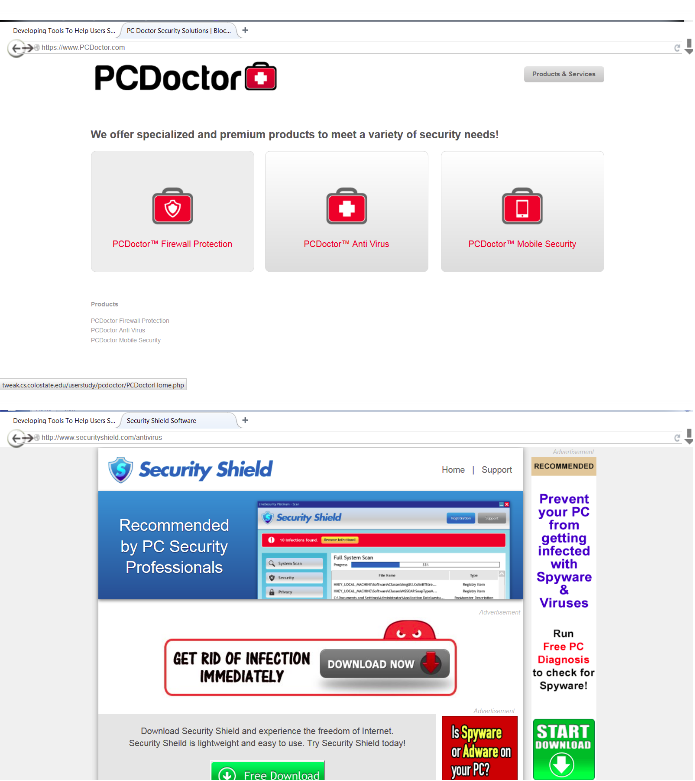
\includegraphics[width=0.7\columnwidth, keepaspectratio=true]{img/virus.png}
  \caption{Simulated Anti-virus download pages: secure anti-virus software (top) and unsafe anti-virus software (bottom)}
  \label{fig:virus}
\end{figure}


\subsection*{Collecting Data}
The system is instrumented to collect subject actions, specifically the start and conclusion of the session, the activation of each activity, typing and mouse clicks in the applications (buttons, widgets, windows, etc.) The results of the pre and post surveys and subject preferences (e.g., software selections, password choices) were also logged using PHP session variables. All activity related data are captured with timestamps.

\subsection*{Experimental Design}
In this study our focus was on two factors common to several well-known models of user security behavior: self-efficacy and cues-to-action (e.g., Health Belief Model, Protection Motivation Theory). The core idea was to ask questions related to those two factors, then observe the user actions within scenarios designed to elicit potentially detrimental responses and then to ask questions about the tasks that they had undertaken. Our hypothesis about the comparison of data collection methods is that self-reporting was likely to differ from observed actions. Thus, the study was designed with five parts: an introduction, a pre-study questionnaire, on-line completion of four tasks, a debriefing and a post-study questionnaire. The study was designed as a within-group experiment, where all participants were placed in identical threat scenario simulations. Written instructions were given to all participants to assist them in completing the required set of tasks. Video/audio recordings were not used. The study took approximately 45 minutes to complete.

\subsubsection*{Participants}
We collected data from 61 university undergraduates. The students were enrolled in a psychology course during the semester the study was conducted. The course attracts a wide range of majors and gives research credit for participating in studies. All participants were given informed consent and participated voluntarily.


\subsubsection*{Use of Deception}
We introduced some deception into the study in three ways:
\begin{enumerate}
\item The description of the study used to attract participants indicated that the study was to evaluate their ability to complete common tasks on the computer so that the researchers can
use the findings to develop tools to help users set up their computers.
\item A task, which was unrelated to the focus of the study (i.e., compose and save email as draft)
was added to one of the other tasks to help mask the actual purpose of the study. This task
did not generate any useful data.
\item To induce a sense of buy in, the participants were presented with a cover story at the start of
the study. The cover story stated that the participant had purchased a second hand computer
with Microsoft Windows and one utility application (Mozilla Firefox) installed. Experiment tasks were to study the participants ability to set up this newly purchased computer to be used as an additional computer by multiple users at their home. The cover story was
communicated to participants during the introduction session.
\end{enumerate}

\subsubsection*{Surveys}
We presented two surveys. The pre-study survey shown in Appendix \ref{apx:cypre} asks three questions (questions 1 - 3) about demographics and 10 questions about computer experiences (questions 4 - 13). Although we would have liked to directly assessed self-efficacy, the standard questions, as pioneered by \cite{ng2007, claar2010}, asked about level of confidence when executing specific tasks in different contexts. We did not wish to prime the participants to be thinking about computer security during the on-line portion of the study. Instead, we followed the tone of Mannan and van Oorschot \cite{mannan2008}, which asked about their experience with computers (questions 4 - 8), what challenges they perceive (question 9), where they obtain help (questions 10 - 11) and what software they have installed (questions 12 - 13). These questions were selected to relate more clearly to the cover story.

For the post-study survey (Appendix \ref{apx:cypost}), we adopt the standard survey instruments, which evaluate self-efficacy for computer security practices from \cite{ng2007, compeau1995}. Instruments that measure cues-to-action are adopted from \cite{ng2007}. It must be noted that our idea of cues refer to security notifications available in the computing environment such as SSL lock icon in URLs, web site content/look and feel as opposed to external information sources like news, help-desks etc. in Ng et al.\cite{ng2007}. Questions 2 - 11 evaluate the self-efficacy of the anti-virus software usage. Questions 12 - 19 evaluate self-efficacy of safe communication over social media (Twitter). Questions 21 - 24 evaluate self-efficacy of using email and managing passwords. Questions 20, 25-29 are about awareness of secure and private information collection. Questions 30 - 35 evaluate cues-to-action on practicing computer security on the Internet. The first question asks for the pseudonym which allows us to connect the on-line portion's data with the post-survey data. The main purpose of these questions was to establish whether or not the actions in the online portion of the study corresponded to what they thought that they did.


\subsubsection*{Experiment Protocol}
Figure~\ref{fig:tasks} illustrates the experiment protocol.
\begin{figure}[ht]
  \centering
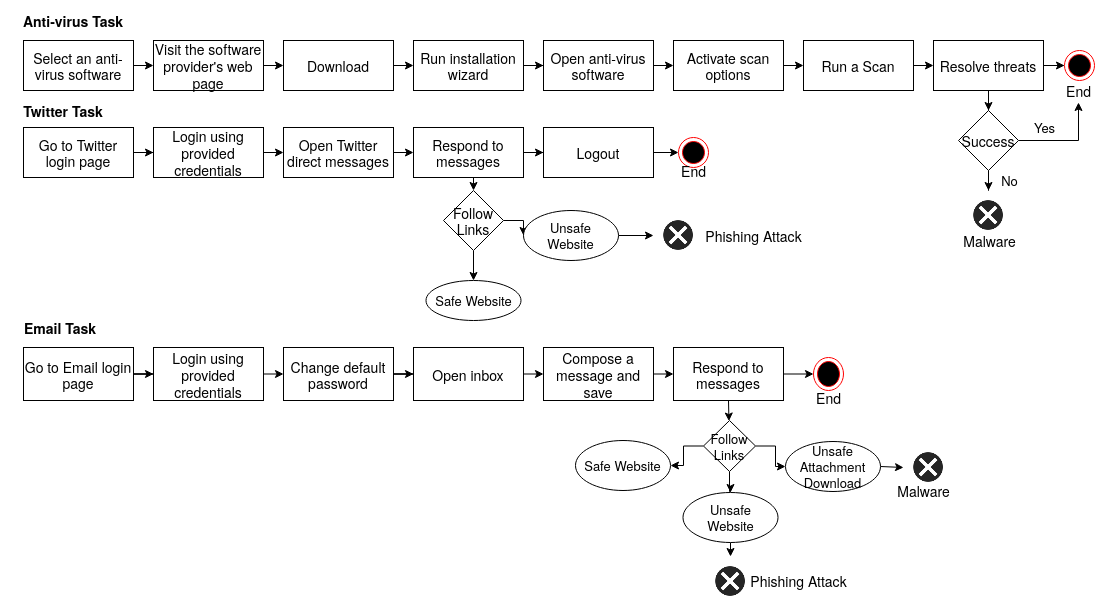
\includegraphics[width=1.1\columnwidth, keepaspectratio=true]{img/tasks.png}
  \caption{Sandbox task breakdown}
  \label{fig:tasks}
\end{figure}
When the participants arrived for the study, one person checked their name on an attendance list, and randomly assigned a username and password to login to a desktop machine. Upon logging in, the participants were presented with a screen that described and organized their on-line tasks.  In the first scenario, participants were directed to install, configure and run anti-virus software as part of setting up their new machines.  

A mock-up version of a popular social media application (Twitter) was implemented for the purpose of studying users' communication habits. In this activity, users were instructed to use a private messaging feature of Twitter. Users were shown three private messages: two legitimate, safe messages sent from trustworthy sources (different offices within the university at which the study took place) and one phishing message. All messages contained URLs. The URL in the phishing message directed users to a phishing website \texttt{bit.ly/UAZou2}, where they were prompted to enter their username and password. In their instructions, they were told that this task would allow them to check that Twitter was working correctly on the computer; they were asked to login, read messages and ``take appropriate action''.


A web based email client was used for the email scenario. Users were given personal email accounts and a common default password designated for the study. They were told ``The email account is unique to you. However, the default password is being shared by all users of the computer.'' The email task comprised two sub tasks. First, to study their ability to choose strong passwords, participants were instructed to change the default password of their email accounts to a new password of their choice. Second, users were instructed to compose a new email message, read email messages and respond to unread messages. Three new messages were placed in the inbox: one safe message and two unsafe messages. One of the two unsafe messages was a phishing message with a URL that would direct the user to a phishing website upon clicking. The phishing website was masked as the web-mail client itself. The other unsafe message contained an attachment: a harmful zip file. The message content was patterned after actual phishing email messages. The phishing websites and zip file attachments were mock-ups within the sandbox; thus, they did not pose an actual security threat to the computer or to the participant's personal data. 
If the user followed any unsafe task that resulted in compromised security, the system displayed a message that the computer system's safety is now compromised.


Once the participant finished the tasks, he/she was directed to the post-study survey and a debriefing explanation. We also offered them the opportunity to further discuss the debriefing with one of the staff conducting the study.


\subsection*{Summary of Findings}
\subsubsection*{Pre-Survey Findings}
Although the participants had a lot of prior experience with computers (66\% with more than 9 years), they had little formal training (59\% had none) and turned to the Internet for help as their primary source (92\%). Most (82\%) owned multiple devices. Nearly all (95\%) had installed multiple applications, i.e., Chrome, Office, Flash, Skype and Acrobat. Given the participant recruitment method, it was not surprising that nearly all had laptops and used their computers for educational activities. With respect to computer security, more than half (67\%) found it challenging to identify harmful actions and take steps to ensure safety. Yet most (77\%) had anti-virus software on their computers. Pre-survey questionnaire is shown in Appendix~\ref{apx:cypre}.

\subsubsection*{Post-Survey Findings}
In our post-survey, the Questions 2 - 24 and 30 are answered on a 5 point scale and are encoded from 1 to 5 (higher is better). For questions 3 - 11, 13 - 24 and 30, from Strongly Disagree to Strongly Agree. For questions 2 and 12, the answers varied from Very Hard to Very Easy. Questions 25 - 29 allowed answers of ``Yes'', ``No'' and ``I don't know''. Questions 33 and 35 allowed ``Yes'' and ``No''. Questions 31, 32, and 34 had categorical answers. Post-survey questionnaire is shown in Appendix~\ref{apx:cypost}.


For the antivirus task, the highest level of confidence was in configuring and using the antivirus software. The lowest was in removing suspicious files without help, but even here, they still felt more confident than not (values greater than 3 which is neutral). Questions 6 and 7 (see below) distinguish ability with and without help. A paired sample T-test comparing the responses to questions 6 and 7 shows a significant difference (p < 0.014), which suggests that many participants were concerned about their ability to perform the task on their own. 

\noindent\fbox{%
    \parbox{\textwidth}{%
\begin{enumerate}[label=\arabic*)]
  \setcounter{enumi}{5}
\item I feel confident in my ability to identify and remove suspicious files on my computer using an antivirus software.\vspace*{-1em}
\item I feel confident in my ability to identify and remove suspicious files on my computer using an antivirus software without help.
\end{enumerate}
    }%
}

The participants are a little more confident in their use of Twitter than the antivirus tasks. The highest level of confidence was in responding to messages; the lowest was in checking links. Paired sample T-tests comparing the responses to questions 14 with 15 and 14 with 16 (see questions below) show no significant difference (P > .09).

\noindent\fbox{%
    \parbox{\textwidth}{%
\begin{enumerate}[label=\arabic*)]
  \setcounter{enumi}{13}
\item I feel confident in my ability to identify suspicious messages on Twitter.\vspace*{-1em}
\item I feel confident in my ability to identify suspicious messages on Twitter without help.\vspace*{-1em}
\item I feel confident in my ability to identify suspicious messages on Twitter even if it is the first time I had seen one.
\end{enumerate}
    }%
}


The participants are confident in their use of email. The highest level of confidence was in choosing a strong password; the lowest was in the security warnings. Paired sample T-tests comparing the mean confidence ratings to questions 21 with 22 (see questions below) shows no significant difference (P > 0.71).

\noindent\fbox{%
    \parbox{\textwidth}{%
\begin{enumerate}[label=\arabic*)]
  \setcounter{enumi}{20}
\item I practice caution when responding to email from senders I am not familiar with.\vspace*{-1em}
\item I practice caution downloading attachments in emails from senders I am not familiar with.
\end{enumerate}
    }%
}

\subsubsection*{Between Sandbox and Post-Survey Findings}
We now compare the users' actual sandbox activities against what they reported in the post-study survey for the three tasks: using anti-virus, communicating on Twitter and email communication.


The anti-virus task consisted of three sub-tasks: (1) given a legitimate and an illegitimate antivirus software, the user was asked to choose one (choice), (2) install the selected software and configure it to be used in the computer (install) and (3) run the software on the computer and remove threats (scan). In the post-survey, question 4 measures self-efficacy of the choice, question 9 measures the self-efficacy of the install and question 6 measures the self-efficacy of the scan. See below for questions 4, 6, and 9 from Appendix~\ref{apx:cypost}. From the 62 participants only 11 completed all three sub-tasks, while 32 participants skipped the anti-virus task altogether. Those who did not complete the task skipped the install or scan or both. All 11 participants who completed all three sub-tasks installed the legitimate anti-virus software. This shows that users who practice computer security typically execute similar actions when they are placed in similar situations.

\noindent\fbox{%
    \parbox{\textwidth}{%
\begin{description}
\item [4)] I feel confident in my ability to select an antivirus software that matches my security requirements.\vspace*{-1em}
\item [6)] I feel confident in my ability to identify and remove suspicious files on my computer using an antivirus software. \vspace*{-1em}
\item [9)] I choose an antivirus software, which allows me to customize its features to match my security requirements.
\end{description}

    }%
}

The two-tailed T-test that compares the self-reported efficacy between those who completed the choice task and those who did not is significant (P > 0.05). The same can be observed for the scan activity. However, the self-reported efficacy is not significant for the install task. This shows that for certain tasks that involve anti-virus software usage, users can incorrectly assess their self-efficacy when practicing computer security in self-reports.

Our post survey contained 3 questions (questions 14 - 16), which evaluated self efficacy of communicating safely on Twitter. All 61 participants who completed the task opened/responded to at least one of the three messages.

The two-tailed T-test that compares the self-reported efficacy between those who visited the phishing web page following the link that appeared on their Twitter direct message and those who did not. It can be seen that the participants evaluated their self efficacy to recognize phishing attempts while communicating on Twitter higher than it actually was. There is no significant difference between the self-efficacy ratings for the participants who clicked the phishing link and the participants who did not, P > 0.05 for all questions.

Users found it difficult to correctly assess their self-efficacy in practicing caution when communicating with email. Questions 21 and 22 in the post-survey asked users to rate their self efficacy. When encountered with an email containing a phishing link, two tailed T-test showed that there is no statistical significance between self-efficacy ratings given by users who did not follow the phishing link against the users who did (P > 0.05). All users, who visited the phishing link, except one submitted their login credentials to the phishing web site. The users who submitted their login credentials had a mean self-efficacy rating 3.89 (SD=0.90). Similar observation can be made from users who downloaded malicious attachments that come with email. Two tailed T-test revealed that there is no statistical significance (P > 0.05) between the self-efficacy ratings given by users who downloaded malicious attachments  from email against the users who did not.


\subsection*{Significance of the Study to Intervention}
Our objective of this study is to highlight that regardless the perceived self-efficacy and availability of cues, human users can still end up compromising their security. In certain situations, if the user is not interrupted, they could end up putting their safety in even more risk.

We identified important conditions that should be addressed when designing an intervention system to help human users. First, even though users were given step-by-step instructions for completing these task, they rarely follow the script. There were repeated as well as omitted actions. This means monitoring users to help them avoid unsafe consequences need to handle noisy and/or missing actions. Furthermore, any partially complete task (a partial plan) that has been safe upto now may quickly turn unsafe. This means that the intervention decisions need to be made online. Users perform a large number of actions; while few of them incur much risk, some are pivotal in triggering vulnerabilities.

Second, in order to determine the safety of an action, we need to evaluate how close the user is to the undesirable state irrespective of the user's goal because users have trouble sticking to one specific goal, which maybe hard to identify. Therefore this becomes an assessment between how critical the observed action to trigger likely undesirable outcomes and whether an action is likely to lead to undesirable outcome, immediately or as part of an action sequence, or may provide conditions that an attacker can exploit.  Thus we need a model of actions (user actions and system actions), which describes how vulnerabilities can manifest in the computer system with direct and indirect involvement of the user.



\subsection*{Cyber-security Planning Domain Model}
We defined a domain model for the cyber-security domain using PDDL (Planning Domain Definition Language) shown in Figure \ref{fig:cybersecdomain}. In total this domain model has 45 actions, 47 types, 70 constants and 55 predicates. This model captures the threat scenarios in the human subject study protocol.

\begin{figure}[pbt]
\noindent\fbox{
 \parbox{\textwidth}{\raggedright: 
{\small
\texttt{(define (domain attackgraph-typed)}\\
\texttt{\hspace*{35pt}(:requirements :strips :adl :equality :typing \hspace*{35pt} :disjunctive-preconditions)}\\
        \hspace*{35pt}\texttt{(:types unknown software misc - object)\\
       \hspace*{35pt} \texttt{account certificate email-ID file key site user attacker vulnerability-type password direct-message device database parameter permission process username response request - misc}\\
\hspace*{35pt} \texttt{browser editor webmailer plug-in site-creating-software server-connecting-software server anti-virus OS desktop-app server-app malicious-software - software}\\
\hspace*{35pt} \texttt{phishing-site server-site normal-site - site}\\
\hspace*{35pt} \texttt{phishing-site-email phishing-site-twitter - phishing-site}\\
\hspace*{35pt} \texttt{attacker-remote attacker-local - attacker)}
        }\\ [15 pt]
\hspace*{35pt}\texttt{(:constants \\ 
\hspace*{35pt}user1-email-account user1-twitter-account - account \\
\hspace*{35pt}pc-doctor security-shield - anti-virus \\
\hspace*{35pt}browser-firefox - browser \\        \hspace*{35pt}phishing-direct-message - direct-message \\
\hspace*{35pt}email-with-malicious-attachment - email-ID\\
\hspace*{35pt}squirrelmail - webmailer\\
\hspace*{35pt}user1-twitter-password - password $\ldots$ )\\[15 pt]
}
\hspace*{35pt}\texttt{(:predicates \\
\hspace*{35pt}(information-available ?aUser - User ?anAccount - account) \\
\hspace*{35pt}(user-has-email-account ?anAccount - account)\\
\hspace*{35pt}(direct-message-received ?dmsg - direct-message)\\
\hspace*{35pt}(anti-virus-software-selected ?av - anti-virus) \\
\hspace*{35pt}(information-leakage ?anAccount - account $\ldots$ )\\[15pt]
}

\hspace*{35pt}(\texttt{:action user-visit-antivirus-download-site}\\
\hspace*{35pt}\texttt{:parameters (?U - user ?aBrowser - browser ?aSite - site \\\hspace*{35pt} ?av - anti-virus)}\\
\hspace*{35pt}\texttt{:precondition ( and (logged-onto-system ?U) \\\hspace*{35pt} (use-software ?aBrowser) (running ?aBrowser) \\\hspace*{35pt} (= ?aSite antivirus-software-download-site) \\\hspace*{35pt} (not (installed ?av))  (not (running ?av)) )}\\
\hspace*{35pt}\texttt{:effect (and (user-visits-site ?U ?aSite))}
)\\[15pt]

\hspace*{35pt}\texttt{(:action user-opens-attachment-through-webmail}\\
\hspace*{35pt}\texttt{:parameters (?U - user ?aBrowser - browser ?WM - webmailer \\\hspace*{35pt}?aSite - site  ?anAccount - account ?Msg - email-ID  ?F - file )}
\hspace*{35pt}\texttt{:precondition (and  (use-software ?aBrowser) (running ?aBrowser) \\\hspace*{35pt}(user-visits-site ?U ?aSite) (= ?aSite webmail-site)\\\hspace*{35pt}(user-has-email-account ?anAccount)\\\hspace*{35pt}(= ?anAccount user1-email-account) (msg-opened ?Msg)\\\hspace*{35pt}(mail-attachment ?Msg ?F) (logged-onto-system ?U))}\\
\hspace*{35pt}\texttt{:effect (opened ?F))} 
 )\\\hspace*{35pt}$\ldots\ldots$
}
}
}
\caption{The cyber-security PDDL domain model snippet}
\label{fig:cybersecdomain}
\end{figure}



\section*{Studying Human User Behavior During a Cognitively Engaging Rush Hour Puzzle}
When a human user is learning to use a new software application, it can be helpful to have a passive observer software agent that can intervene to help the user reach his intended goal. This is particularly important when using the software imposes a significant cognitive load on the user and as a result the user's plan to accomplish the intended goal can become vulnerable to unintended actions or events. 

We implemented an online simulation framework, which allowed human users to solve a Rush Hour puzzle without intervention. As the subject performs the puzzle solving task, the system records the events that occur on the interface. These event logs are used to extract unique user behavior patterns that are indicators of the user's puzzle solving aptitude. We use these patterns to define features of users' solutions for the puzzle. Using the feature set, we generate learned models to predict whether or not the user's solution will reach an undesirable state before it actually happens. 


\section*{The Rush Hour Puzzle}
\label{sec:rushhourpuzzle}
%%about the game
The Rush Hour puzzle is a children's game (for ages 8 and above), that is played on a $n \times n$ square grid. Several cars (size=2) and trucks (size=3) are arranged on the board, which has only one exit. Figure \ref{fig:start} shows a sample initial puzzle configuration on a $6 \times 6$ grid. Vehicles T0, $\ldots$, T2 are trucks and C0, $\ldots$, C7 are cars, with C0 being the special target car. The vehicles can only move in the same orientation in which they were initially placed, i.e., vertical vehicles can only move up and down while horizontal vehicles can move left and right. Vehicles can be moved one at a time and into adjacent empty spaces. The objective of the game is to move the vehicles on the board in such a way that the target car (shown in red in Figure \ref{fig:start}) can be moved out of the exit on the right edge of the board. Solution to the Rush Hour puzzle is a sequence of legal moves that transforms the initial board state shown in \ref{fig:start} to the goal state in \ref{fig:end}. For the puzzle shown in Figure\ref{fig:whole}, the shortest solution, if the number of moves is considered as the optimizing criteria, consists of 21 moves. If optimized for the number of vehicles moved, the puzzle can be solved optimally by moving only 8 vehicles. 
\begin{figure}[!pbt]
  \centering
  \subfloat[Initial game state]{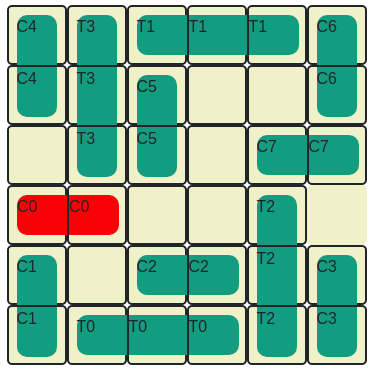
\includegraphics[width=0.4\textwidth]{img/start.png}\label{fig:start}}
  \hfill
  \subfloat[End game state]{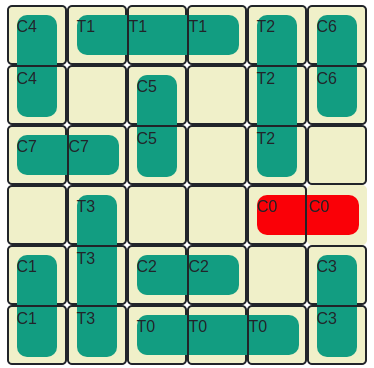
\includegraphics[width=0.4\textwidth]{img/end.png}\label{fig:end}}
  \caption{Rush Hour Board Configurations}
  \label{fig:whole}
\end{figure}
Flake et al. \shortcite{flake2002} showed that the generalized form of the Rush Hour puzzle (GRH) is PSPACE complete. GRH adopts two modifications to the standard problem. First, the grid size is allowed to be a rectangle of arbitrary width and height. Second, the exit is located at any position on the perimeter of the grid. In our experiments we are using the standard version of the puzzle (i.e., $6\times6$ grid with the fixed exit point). We modified the standard version of the Rush Hour puzzle to simulate the presence of an undesirable consequence by introducing a \textit{forbidden} vehicle.  Any action that moves the forbidden vehicle is set to cause the undesirable consequence. The forbidden vehicle introduces a constraint to the set of possible moves the user can make.



\subsection*{The Rush Hour Web Simulator}
We designed the Rush Hour software framework for conducting human subject studies in an environment that allows the user to be engaged in a cognitively taxing task. Our first design choice was in establishing the physical setup of the system. Because the experiments are targeted toward all kinds of computer software users (experts/non-experts), we wanted the subjects' attention to be mainly on the puzzle solving task and not be distracted by a complex user-interface. To allow for more users to participate, while minimizing the time commitment and the effort, we wanted the system to be accessible from anywhere (e.g, home, university etc.). Because of these reasons we designed the system to be a single page web application.

The user interacts with four components: (1) consent agreement, (2) Rush Hour Tutorial, (3) Solver (Board), and (4) Post-study survey/Debriefing. The components are displayed as tabs on the web page.
The solver component allows the user to start a puzzle solving task by clicking a button, at which point a random Rush Hour puzzle is fetched from the server. The participant can move the vehicles on the grid by first clicking once on the vehicle to select it and then clicking once on an adjacent empty cell to move it to the selected cell. To comply with the classical planning model of discrete actions, the application forces the user to move the vehicles one step at a time. 

When choosing Rush Hour puzzle configurations for the study, we want to carefully balance the puzzle's difficulty for a human user. Especially, given the PSPACE-completeness of the (generalized) puzzle, we need the puzzles to be solvable by human users in a reasonable time. Further, we use the Rush Hour puzzle as a supplementary task comparable to human users learning to use a new software or a web application. Therefore, the puzzle solving task should pose a sufficient challenge for the user during the search for a solution in order to make the intervention step more meaningful. We introduce a forbidden vehicle, which must not be moved to each puzzle to restrict the moves the user is allowed to make. This is an alternative way to increase the difficulty of the puzzle without having to increase the number of vehicles on the board \cite{fernau2003}. In order to further instill the importance of avoiding the forbidden vehicle in the user's mind, we also provided warning messages on the Web interface (see the yellow information bar in Figure \ref{fig:ui} panel 2/3) to inform the user about the presence of a forbidden vehicle and what will happen should the forbidden car was moved. However, the users \textbf{are not} explicitly told what the specific forbidden vehicle is.
Figure \ref{fig:ui} shows the web application interface: the tutorial tab, play tab before the user starts the puzzle and when the puzzle is loaded in that order.
\begin{figure}[!hbt]
  \centering
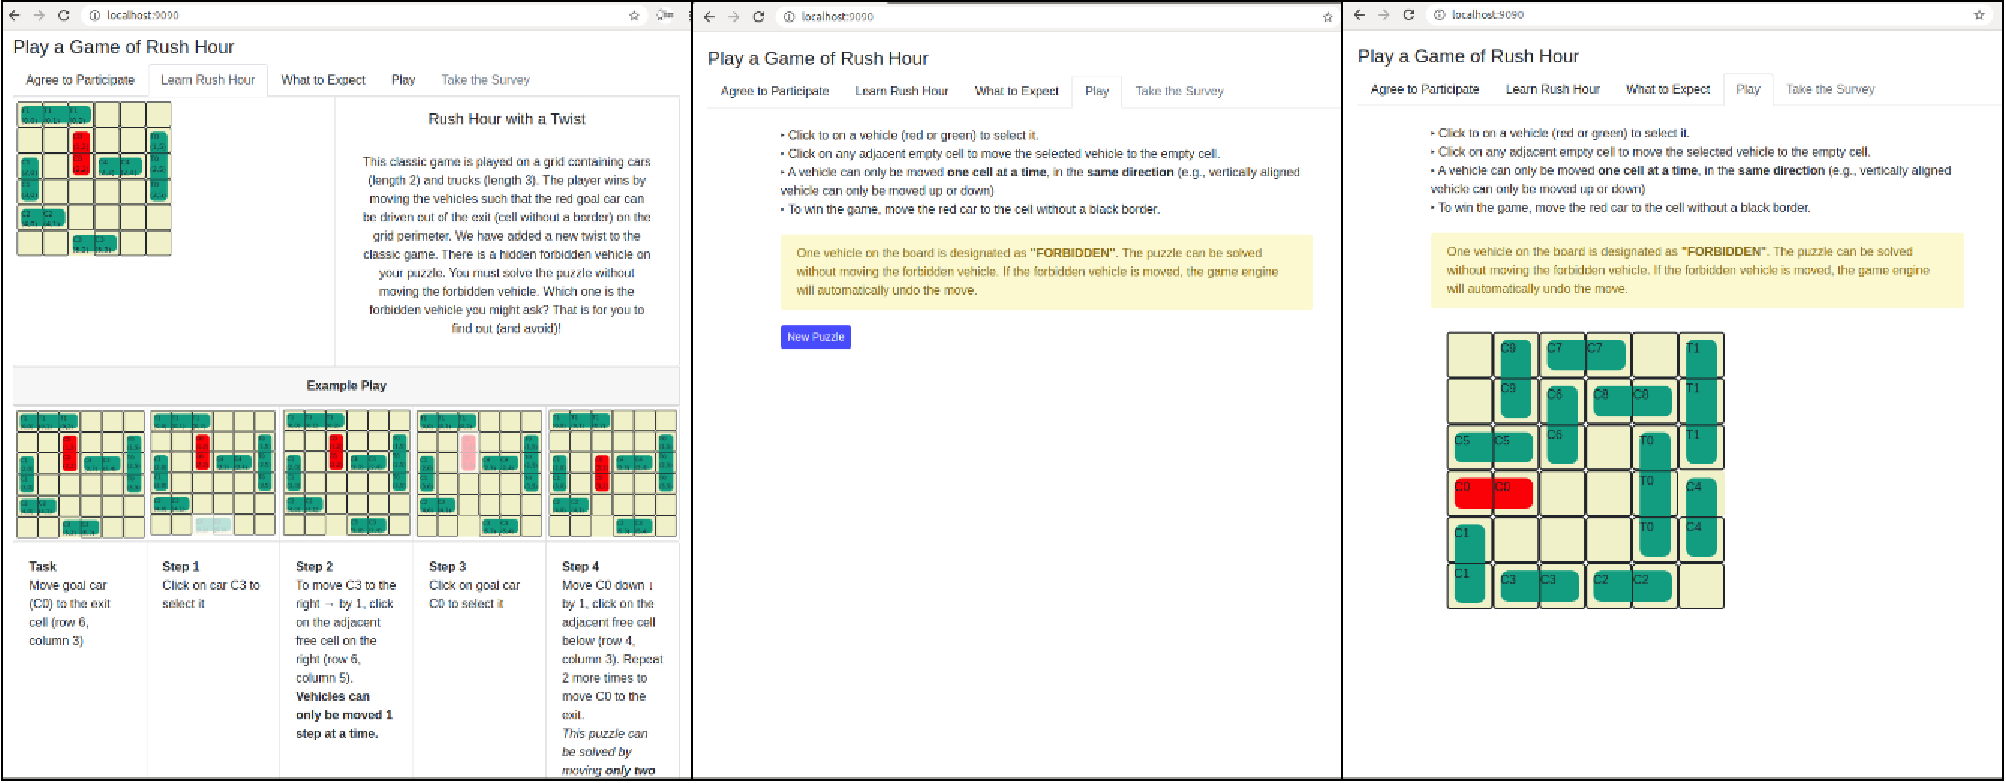
\includegraphics[width=\columnwidth]{img/UI.pdf}
  \caption{Rush Hour Simulation Framework Web Interface}
  \label{fig:ui}
\end{figure}



\subsection*{Collecting Data}
\textbf{Phase 1 - Without Intervention}\\
For each participant, we collect the solution to the Rush Hour puzzle and the demographic information. Data collection is complete. Data analysis is now in progress.

\textbf{Phase 2 - With Intervention}\\
For each participant, we will collect the user's solution to the Rush Hour puzzle, the demographic information and the rating for helpful tips in a 5-point Likert scale. This phase is not complete.

\subsection*{Experimental Design}
\textbf{Phase 1 - Without Intervention}\\
In the first phase of the study, the application user solves the puzzle without any intervention. Upon agreeing to participate in the study each subject is randomly assigned one puzzle out of ten puzzles. When the puzzle is solved, the subject is directed to complete the post-survey. We did not place any time restriction for the puzzle solving task. Participants were informed that one of the vehicles on the game board is forbidden and the puzzle must be solved without moving the forbidden vehicle. However, in this phase we did not give any visual cues (error messages, blocks) to the user in case they happen to move the forbidden vehicle during game play. 

We conducted a pilot study using nine graduate students to assess whether the human solvers were able to solve the selected puzzles within a reasonable amount of time. The pilot study participants solved their assigned puzzles within 5 - 10 minutes. The pilot study participants were also interviewed informally to get their perception of the puzzle difficulty. The participants commented that the puzzles were ''\textit{challenging}'' and "\textit{forced me to think}".

\textbf{Phase 2 - With Intervention}\\
In the second phase, the application intervenes the user and provides helpful hints. Upon agreeing to participate in the study each subject is assigned one puzzle randomly out of 13 puzzles (10 from phase 1 plus 3 new puzzles). In addition the participants are randomly selected to watch a 44 second video of a sample game play. During the game play, the participant is shown five hint types. The participant can follow a hint or decide to ignore it. Once the puzzle solving task is completed, the participants are asked to complete a short survey to capture the demographics and also asks them to subjectively rate the helpfulness of each hint type on a 5-point Likert scale. 

\subsubsection*{Participants}
\textbf{Phase 1 - Without Intervention}\\
We recruited subjects from a graduate and undergraduate university student population. 136 participants completed the study. The sample comprised of college undergraduate and graduate students in Computer Science, Psychology, Agriculture and Business majors. 117 of the 136 participants also completed the demographics survey.

\textbf{Phase 2 - With Intervention}\\
We will recruit subjects from a graduate and undergraduate university student population.

\subsubsection*{Summary of Findings}
\textbf{Phase 1 - Without Intervention}\\
Majority of the participants (39) were below the age of 20, while 38 subjects were between the age 20-25. Maximum age was 41 years. 70 of the 117 participants were male. When asked if they liked puzzle solving tasks, 78\% of the participants either agreed or strongly agreed with the statement. Specifically to the Rush Hour game 79\% of the participants liked or strongly liked Rush Hour. The most common reason as to why the participants liked puzzle solving tasks was that puzzle solving stimulates critical thinking skills. 30\% of the participants usually did a puzzle solving task once a month, while 21\% of the participants solved a puzzle once a week.

When asked about strategies the participants used to solve difficult puzzles, 79\% of the group said that they kept trying until the puzzle was eventually solved, while 12\% of the participants said that they would ask for help.  Given a new puzzle that they have not seen before, if they get stuck while solving the puzzle, 26\% said that they would not like any outside help. 47\% of the participants said that they would like a suggestion/tip that would get them past the current situation. 15\% said that they would like a warning, which indicated that their current approach would lead to a dead-end. 8\% of the participants said that they would like a warning and an explanation to help them prevent getting stuck in the future.  

\begin{figure}[htb]
  \centering
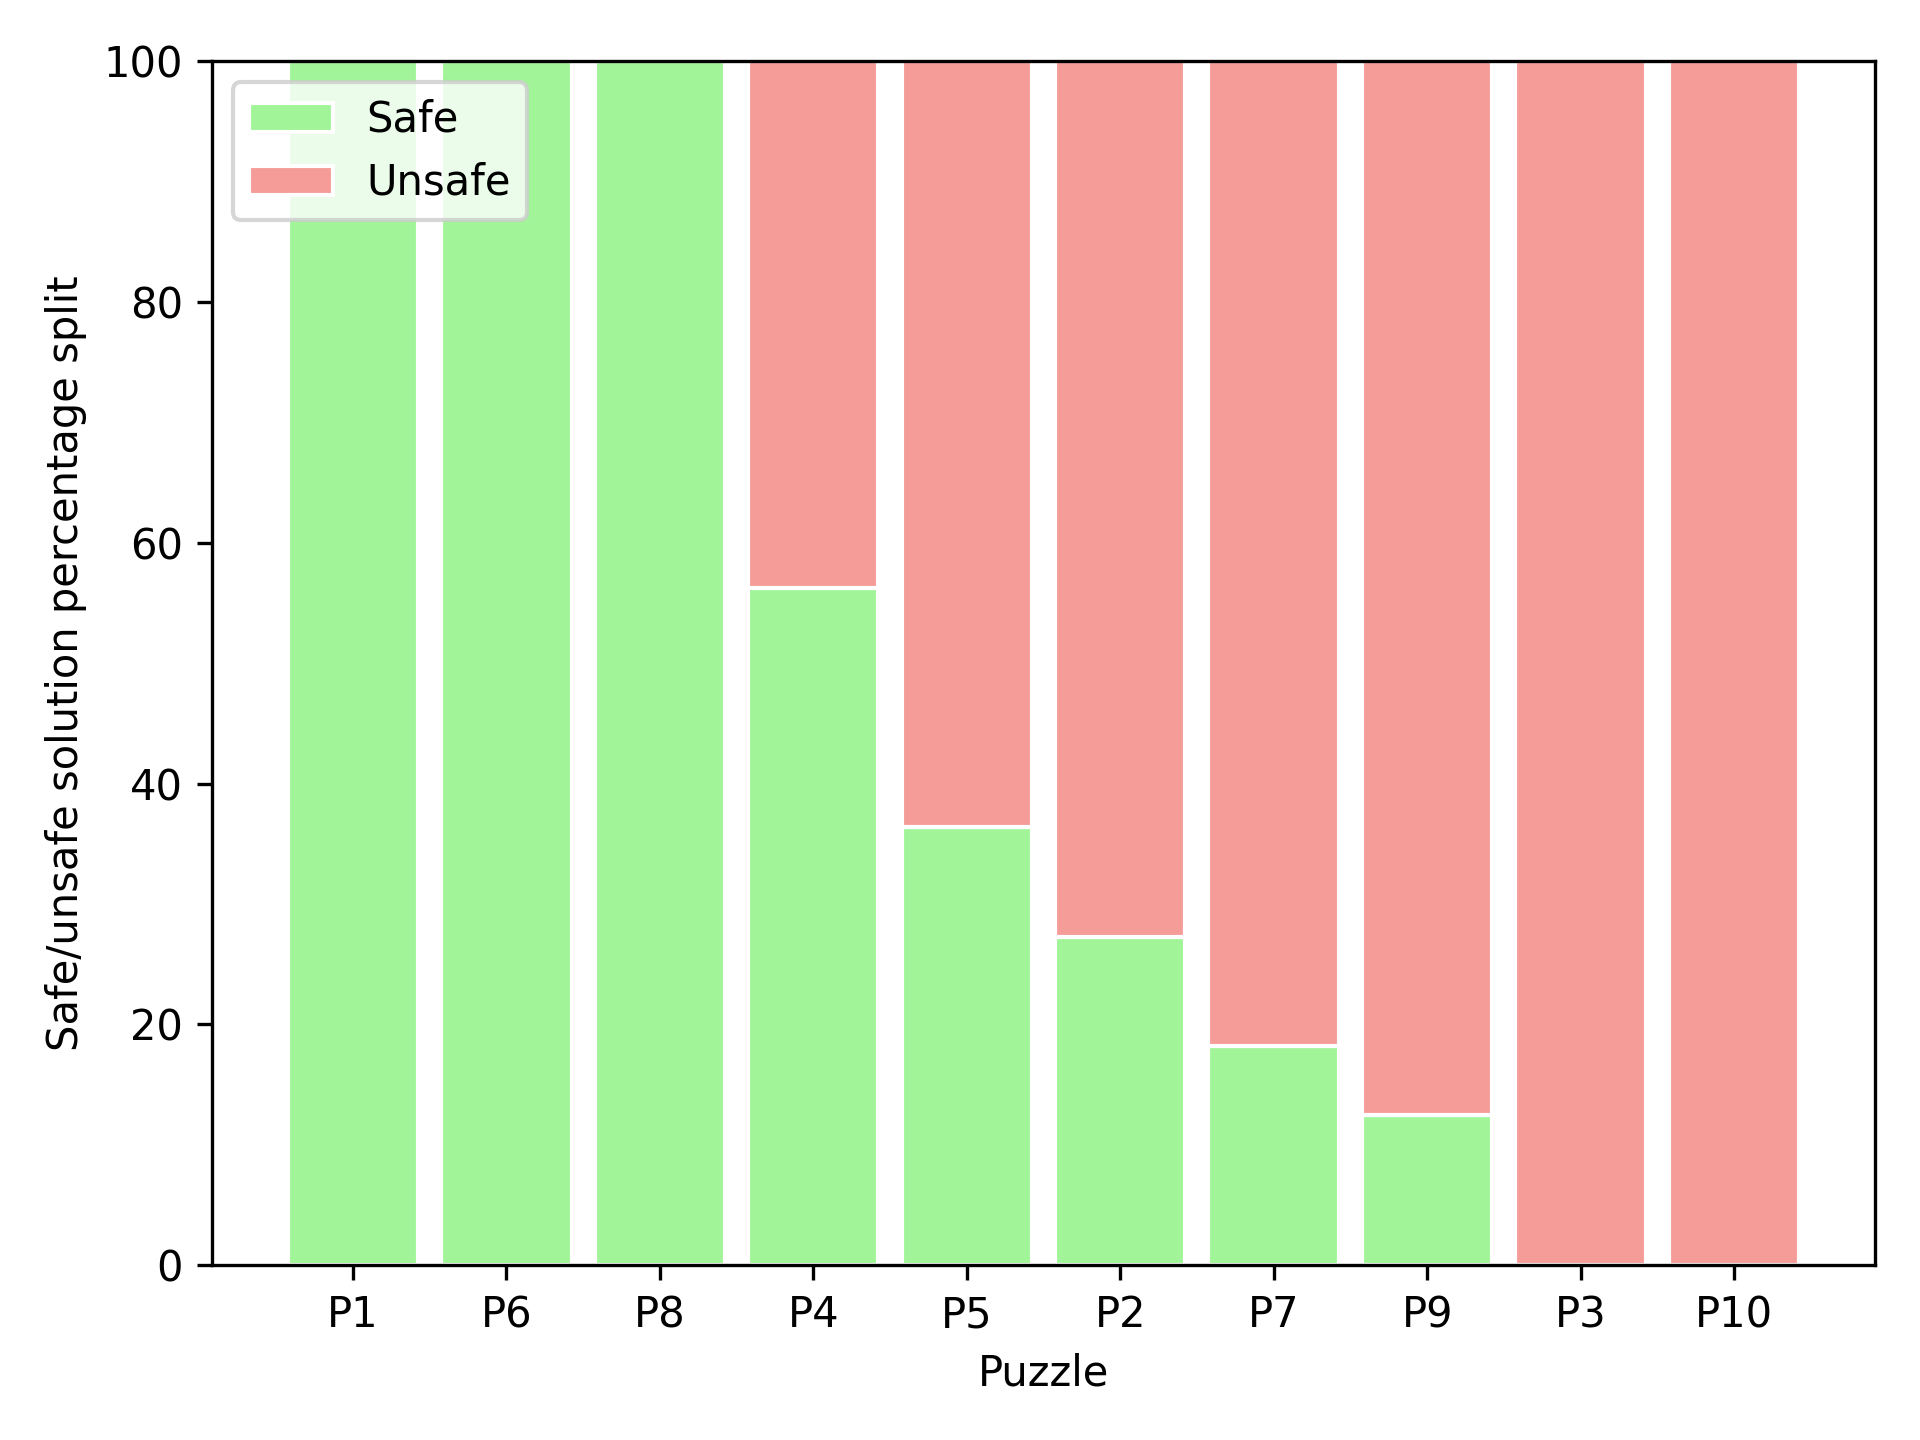
\includegraphics[width=0.5\columnwidth]{img/p2.png}
  \caption{Percentage split between unsafe and safe solutions produced by human users for puzzles P1 through P10}
  \label{fig:split}
\end{figure}


From the 136 subjects, 66 produced solutions that involved moving the forbidden vehicle. From those who moved the forbidden vehicle, 54 users moved the vehicle more than once. Mean number of moves was 53 ($SD=55$) for the sample and maximum number of moves was 378. Table \ref{tab:usersolutions} describes the summary statistics for safe and unsafe solutions produced by the human solvers. 

\begin{table}[htb]
\begin{tabular}{|l|l|l|l|l|l|l|l|l|l|l|}
\hline
\multicolumn{1}{|c|}{\multirow{2}{*}{PID}} &
  \multicolumn{5}{c|}{Safe Solutions} &
  \multicolumn{5}{c|}{Unsafe Solutions} \\ \cline{2-11} 
\multicolumn{1}{|c|}{} &
  \multicolumn{1}{c|}{Freq} &
  \multicolumn{1}{c|}{Min} &
  \multicolumn{1}{c|}{Max} &
  \multicolumn{1}{c|}{Mean} &
  \multicolumn{1}{c|}{SD} &
  \multicolumn{1}{c|}{Freq} &
  \multicolumn{1}{c|}{Min} &
  \multicolumn{1}{c|}{Max} &
  \multicolumn{1}{c|}{Mean} &
  \multicolumn{1}{c|}{SD} \\ \hline
P1  & 18 & 24 & 106 & 43.9  & 20.5  & -  & -  & -   & -    & -    \\ 
P2  &  3  & 44 & 158 & 99.3 & 57.1 & 8  & 78 & 378 & 190.3 & 120.0\\ 
P3  & -  & -  & -   & -     & -     & 12 & 25 & 50  & 35.5 & 8.3  \\ 
P4  & 9  & 23 & 46  & 30    & 7.1   & 7  & 25 & 124 & 67.4 & 33.9 \\ 
P5  & 4  & 23 & 32  & 26.5  & 3.9   & 7  & 14 & 82  & 32.0 & 23.3 \\
P6  & 14 & 22 & 55  & 29    & 10.3  & -  & -  & -   & -    & -    \\
P7  & 2  & 29 & 37  & 33    & 5.7   & 9  & 43 & 132 & 80.9 & 38.2 \\ 
P8  & 18 & 9  & 12  & 9.3   & 0.8   & -  & -  & -   & -    & -    \\
P9  & 2  & 21 & 27  & 24    & 4.2   & 14 & 29 & 169 & 66.3 & 39.0 \\
P10 & -  & -  & -   & -     & -     & 9  & 44 & 158 & 81.2 & 39.2 \\ \hline
\end{tabular}
\caption{Frequency, minimum, maximum, mean and std. deviation number of moves in users' solutions for the Rush Hour puzzles P1 through P10}
\label{tab:usersolutions}
\end{table}



\subsection*{Rush Hour Planning Domain Model}

We defined a domain model for the Rush Hour puzzle using PDDL (Planning Domain Definition Language). Constants of type direction in the domain model are used to identify movement directions right (\texttt{EW}), left (\texttt{WE}), down (\texttt{NS}), up (\texttt{SN}). The constants of type location identify cells in a $6 \times 6$ grid. The predicates are the state variables that may take the values \textit{True}/\textit{False}. The domain model consists of two actions \texttt{move-car} and \texttt{move-truck}. \texttt{move-car} action is described with the parameter set: car identifier ($C_i$), cell number of the starting position (\texttt{?from}), cell number of the end position (\texttt{?to}), the cell that becomes free after the move (\texttt{?tail}) and the direction of the move (\texttt{?d}). The action \texttt{move-truck} is defined similarly, the only difference being the truck's position is described by three cells (\texttt{?from}, \texttt{?mid}, \texttt{?to}). 

\begin{figure}[!ht]
\noindent\fbox{
 \parbox{\textwidth}{\raggedright: 
{\small
\texttt{(define (domain rush-hour)}\\
\texttt{\hspace*{35pt}(:requirements :strips :typing :universal-preconditions \\ 
\hspace*{35pt}:disjunctive-preconditions)}\\[15 pt]
        \hspace*{35pt}\texttt{(:types location vehicle direction)}\\ [15 pt]
        \hspace*{35pt}\texttt{(:constants  
                EW WE NS SN - direction \\
        \hspace*{35pt}L1 L2 L3 L4 L5 L6 L7 L8 L9 L10 L11 L12 L13 L14 L15 L16 L17 \\
        \hspace*{35pt}L18 L19 L20 L21 L22 L23 L24 L25 L26 L27 L28 L29 L30 L31 \\
        \hspace*{35pt}L32 L33 L34 L35 L36 - location)}\\[15 pt]
        \texttt{\hspace*{35pt}
        (:predicates \\
        \hspace*{35pt}(car ?v - vehicle)\\
        \hspace*{35pt}(truck ?v - vehicle)\\
    \hspace*{35pt}(at ?v - vehicle ?l - location)\\
        \hspace*{35pt}(face ?v - vehicle ?d - direction)\\
        \hspace*{35pt}(free ?l - location)\\
        \hspace*{35pt}(next ?d - direction ?l1 ?l2 - location)\\
        \hspace*{35pt})\\ [15 pt]}
\texttt{\hspace*{35pt}(:action move-car \\
                \hspace*{35pt}:parameters (?v - vehicle ?from ?to ?tail - location \\ \hspace*{35pt}?d - direction)\\
                \hspace*{35pt}:precondition (and (car ?v)(at ?v ?from)(at ?v ?tail)\\\hspace*{35pt}(face ?v ?d)(next ?d ?from ?to)(next ?d ?tail ?from)(free ?to))\\
                \hspace*{35pt}:effect (and (at ?v ?to) (not (at ?v ?tail))(free ?tail)\\\hspace*{35pt}(not (free ?to))))\\[15 pt]}
\texttt{\hspace*{35pt}(:action move-truck \\
                \hspace*{35pt}:parameters (?v - vehicle ?from ?to ?mid ?tail - location \\\hspace*{35pt}?d - direction)\\
                \hspace*{35pt}:precondition (and (truck ?v)(at ?v ?from)(at ?v ?mid)\\\hspace*{35pt}(at ?v ?tail)(face ?v ?d)(next ?d ?from ?to)(next ?d ?mid ?from)\\\hspace*{35pt}(next ?d ?tail ?mid)(free ?to))\\[0.25 pt]
                \hspace*{35pt}:effect (and (at ?v ?to)(at ?v ?from)(at ?v ?mid)\\\hspace*{35pt}(not (free ?from))(not (free ?mid))(not (at ?v ?tail))\\\hspace*{35pt}(free ?tail)(not (free ?to)))))
}
}
}
}
\caption{Rush Hour PDDL Domain Model}
\label{fig:domain}
\end{figure}

Table \ref{tab:plan} shows two plans for the Rush Hour puzzle illustrated in Figure \ref{fig:start}. The safe solution is obtained by an automated planner optimized for the number of moves. The unsafe (partial) solution is produced by a human user. The user's complete solution contains 43 moves. The highlighted step in the unsafe solution (18$^{th}$ move) is a dangerous move because it involves moving the forbidden vehicle \texttt{C2} for this puzzle. In the complete solution, the human user moved the forbidden vehicle twice.

\begin{table}[ht]
\begin{tabular}{|c|c|}
\hline
Safe solution (21 moves) & Unsafe solution (partial) \\
\hline
\begin{tabular}[c]{@{}l@{}}\texttt{\textsc{move-car c0 l17 l16 l18 we}}\\ \texttt{\textsc{move-car c0 l16 l15 l17 we}}\\ \texttt{\textsc{move-truck t3 l23 l17 l29 l35 ns}}\\ \texttt{\textsc{move-car c7 l20 l21 l19 ew}}\\ \texttt{\textsc{move-car c6 l25 l19 l31 ns}}\\ \texttt{\textsc{move-truck t1 l32 l31 l33 l34 we}}\\ \texttt{\textsc{move-car c5 l28 l34 l22 sn}}\\ \texttt{\textsc{move-truck t3 l17 l11 l23 l29 ns}}\\ \texttt{\textsc{move-car c7 l21 l22 l20 ew}}\\ \texttt{\textsc{move-truck t2 l14 l20 l8 l2 sn}}\\ \texttt{\textsc{move-truck t2 l20 l26 l14 l8 sn}}\\ \texttt{\textsc{move-truck t0 l3 l2 l4 l5 we}}\\ \texttt{\textsc{move-truck t3 l11 l5 l17 l23 ns}}\\ \texttt{\textsc{move-car c7 l22 l23 l21 ew}} \\ \texttt{\textsc{move-car c7 l23 l24 l22 ew}}\\ \texttt{\textsc{move-car c5 l28 l22 l34 ns}}\\ \texttt{\textsc{move-truck t1 l33 l34 l32 l31 ew}}\\ \texttt{\textsc{move-truck t1 l34 l35 l33 l32 ew}}\\ \texttt{\textsc{move-truck t2 l26 l32 l20 l14 sn}}\\ \texttt{\textsc{move-car c0 l15 l14 l16 we}}\\ \texttt{\textsc{move-car c0 l14 l13 l15 we}}\end{tabular} &
  \begin{tabular}[c]{@{}l@{}}\texttt{\textsc{move-car c0 l17 l16 l18 we}}\\ \texttt{\textsc{move-car c0 l16 l15 l17 we}}\\ \texttt{\textsc{move-car c4 l30 l24 l36 ns}}\\ \texttt{\textsc{move-car c4 l24 l18 l30 ns}}\\ \texttt{\textsc{move-truck t3 l23 l17 l29 l35 ns}}\\ \texttt{\textsc{move-truck t3 l17 l11 l23 l29 ns}}\\ \texttt{\textsc{move-truck t1 l34 l35 l33 l32 ew}}\\ \texttt{\textsc{move-truck t1 l35 l36 l34 l33 ew}}\\ \texttt{\textsc{move-car c7 l20 l21 l19 ew}}\\ \texttt{\textsc{move-car c6 l25 l19 l31 ns}}\\ \texttt{\textsc{move-truck t1 l34 l33 l35 l36 we}}\\ \texttt{\textsc{move-truck t1 l33 l32 l34 l35 we}}\\ \texttt{\textsc{move-truck t1 l32 l31 l33 l34 we}}\\ \texttt{\textsc{move-car c5 l28 l34 l22 sn}}\\ \texttt{\textsc{move-car c7 l21 l22 l20 ew}}\\ \texttt{\textsc{move-truck t2 l14 l20 l8 l2 sn}}\\ \texttt{\textsc{move-truck t2 l20 l26 l14 l8 sn}}\\ \colorbox{LightSalmon}{\texttt{\textsc{move-car c2 l9 l8 l10 we}}}\\ \texttt{\textsc{move-truck t0 l3 l2 l4 l5 we}}\\ \texttt{\textsc{move-truck t3 l11 l5 l17 l23 ns}}\\ \texttt{\textsc{move-truck t3 l17 l23 l11 l5 sn}}\\ \texttt{\textsc{move-truck t3 l23 l29 l17 l11 sn}}\\ $\ldots$\end{tabular} \\ \hline
\end{tabular}
\caption{Solution snippets for a Rush Hour Puzzle in Figure \ref{fig:start}. Solution on the left is an optimal solution that does not move the forbidden vehicle. The partial solution on the right was produced by a human user and includes a forbidden vehicle move.}
\label{tab:plan}
\end{table}











%%%%%%%%%%%%%%%%%%%%%%%%%%%%%%%%%%%%%%%%%%%%%%%%%%%%%%%%%%%%%%%%
%\chapter{How Do Home Computer Users Behave in Questionable Security Situations?}
%\label{chap:compsec}
%\section*{Introduction}
%The 2016 American Community Survey found that 89\% of all households had a computer, including smartphones making it a common feature of everyday life \cite{ryan2016}. Also, 81\% had a broadband subscription. The Internet impacts many areas of the daily life, from performing routine tasks like shopping, banking to connecting to family and friends via social media. The Internet has become an avenue to pursuing formal education (e.g., online degree programs) as well as informal learning (e.g., how-to videos on cooking, household repairs etc.) and allows us to collaborate across many physical barriers. Whether we realize it or not, we are routinely  deciding whether or not to take risks in security and privacy when we interact with computer systems.
%
%Home computer use, as distinguished from work related or organizationally based computer
%use, is dominated by personal activities (mostly recreational, but some financial and health related) and is not governed by security policies determined by experts. Most security approaches for home users have encouraged them to take preventative or precautionary actions, e.g., installing anti-virus/malware software, hardening passwords \cite{chiasson2008}, backing up information \cite{dupuis2012}. We propose a new approach to help human users interact safely with computer systems. This approach is predicated on the principle that security solutions designed for end users need to assess two information sources: 
%\begin{itemize}
%\item The human user's decision making context and the factors that affect the user's decision making ability
%\item Observational data like system logs and user action sequences.
%\end{itemize}
%One such decision making context, which we will study in this work is when the user unwittingly takes actions that may lead to undesirable consequences (e.g., clicking on links in phishing emails). While computer security and privacy decision making share characteristics of other decision making models about possibility of undesirable consequences, the combination is unique. Thus, theoretical models (e.g., Protection Motivation Theory \cite{rogers1997} and Theory of Planned Behavior \cite{ajzen1991}) applied in other decision-making contexts (e.g., health) fall short in their applicability because they use different models of risk management.
%
%This study makes two contributions:
%\begin{itemize}
%\item Analyses backed by human subject studies relating what human users think is happening to what they actually do. This is critical to understanding how much can be inferred from surveys.
%\item Software framework to support home computer user security/privacy studies. We create a lightweight, sandbox software system, which simulates the Microsoft Windows environment on desktops and laptops. The simulator supports a small set of vulnerabilities and the scenarios that could possibly trigger them.
%\end{itemize}
%
%The decision of when to flag a problem also relies on the knowledge about the user. We refer to this as the user's decision making context. Success will depend on not bothering the user unnecessarily. For example, users who have the skill for recognizing computer security threats like phishing attacks, spoofing attacks and care about the negative consequences of these threats need less monitoring. On the other hand, users who are less aware of the threats require more help. So, the question we need to address is \textit{what type of users make particular computer security decisions}. We answer this question by drawing from health related behavioral models to explain security behavior. Health behavior is a natural analogy to how we respond in cyber-security threats. We frame many related issues in cyber-security using health related metaphors. For example, we refer to viruses and infections when talking about cyber attacks, we discuss system hardening after an attack takes place. In this work, we study two specific user characteristics from a health related behavior model called the Health Belief Model (HBM): \textit{self-efficacy}, that is an individuals confidence in her/his ability to perform a security enabling task on the computer, and \textit{cues-to-action}, that is an individual's response to external triggers for how they would affect users practicing computer security. HBM is focused on user's attitudes and beliefs. The user's beliefs are described based on their perceptions of six factors, susceptibility, severity, benefits, barriers, cues-to-action, and self-efficacy of performing a given health behavior \cite{rosenstock88}. We are adopting the HBM for studying user characteristics that affect computer security decision making because the HBM and specifically self-efficacy and cues-to-action have been studied in prior work, which looked into computer security practices of the home user. Studies on self efficacy find that \cite{urbanska2013,aytes2004,milne2009} knowledge about how to practice safe computing increase the rate of safe behavior. However, having knowledge alone does not guarantee practice of computer security. For example, rapid advances in new security technologies make it harder for user to keep up with the latest updates that must be made to ensure safety of his computer. Typically, cues-to-action triggers are advice received from external entities like friends, co-workers, media reports, laws and regulations etc. Studies on cues-to-action \cite{claar2010,ng2007} find that these types of cues do not have a significant effect on human users practicing computer security.  However, these studies mainly use self-reports to evaluate the effects of self-efficacy and cues-to-action on users' decision making. In this work, our objective is to find out whether the same effects can be observed from human users practicing computer security in a simulated home computer environment. Furthermore, the simulated environment allows us to present cues to users that can be monitored easily such as HTTPS/HTTP web sites and safe/unsafe hyperlinks. This enables us to measure user responses to measurable cues as opposed to cues obtained from external sources, which are often hard to monitor and control.
%
%
%The work by Davison and Sillence \cite{davinson2010} show that human users' security related behavior often does not match their stated intentions. Human users often state the intention of being secure online but than perform actions that put their system at risk. Furthermore, studies that have been able to verify user's reports on their computers have uncovered lower actual than reported rates of some behaviors \cite{govani2005, national2010}. Therefore, developing user-friendly security solutions requires observing users performing actions rather than relying on self reporting, which acts as a proxy for actual behavior. Ideally, the home computer user should be studied at home for an extended period of time to be able to accurately gauge the computer security related behavior patterns. However, these requirements pose many logistical and practical problems. For example, the software system used in such studies should be a background process with minimal intrusion to the user's normal computing activities while collecting the necessary system/behavior information at different levels of granularity (e.g., system calls, process information, user action sequences). Knowledge of having these computer security monitoring software installed in their personal computers may force users to practice computer security more thoroughly than they would normally, which will lead to artificial behavior data.  Therefore, we need to balance collecting high quality information against privacy and practicality of studies. The sandbox environment is designed to address the problem of collecting reliable data from human users when practicing computer security. Using the sandbox environment, the subject is asked to walk through a protocol (task list) in a controlled environment, in which they are presented with different decisions to be made and actions taken. The scenarios can be designed to test the effect of cues and responses of users, thus allowing us to study computer security practices without having to only rely on self reports. 
%
%
%
%
%
%
%\section*{Related Work}
%\subsection*{User Behavior for Computer Security}
%Before effective interventions can be developed, we must understand what types of users make particular decisions, and how they prefer to make decisions. What are the factors that influence user's decision making? Studies that have tried to answer this question have used behavioral models as a guide. Like HBM, there are many other behavioral models that have been adopted to study human user behavior such as Theory of Planned Behavior \cite{ajzen1991}, Extended Parallel Process Model \cite{witte1992} and Precaution-Adoption Process  Model \cite{weinstein2002}. These models define constructs that collectively represent a person's actual control over the behavior. Studies that apply these models to explain user behavior in computer security have looked at computer security practices such as password management, email usage, backing up data, antivirus software and firewall usage in both home and organizational environments. Typically, the studies evaluate the effects of the model's constructs on practicing security using self reported surveys from human subjects. Howe et al. \cite{howe2012psychology} observed that most studies that look into computer security practices of users relying on self reported surveys suffered from issues such as respondent bias, socially desirable responding and peer perception. The authors posited that experiments based on simulation, which place the participant in the actual situation that is monitored can help reduce such issues and also be leveraged to assess the emotional reactions of users to interventions and warnings. In this study, we develop a software system that simulates common computer security scenarios to study human behavior in situ.
%
%
%As discussed in the previous section, users adopting computer security concepts share many similarities with how they respond in a health related scenario. For example, consider a user installing an antivirus software to protect his computer against malicious. This is very similar to someone adopting a healthy diet to avoid diseases. HBM, developed in the 1950s after the failure of a tuberculosis screening program attempted to explain and predict health behaviors. HBM consists of six core constructs that affect an individual's core beliefs on some health related concept. These constructs are: susceptibility, severity, benefits, barriers, cues-to-action, and self-efficacy of performing a given health behavior. Let us translate the HBM for a scenario where the user is trying to protect his computer against a virus attack using antivirus software. HBM states that the user's behavior will depend on the user believing that there is a high probability that his computer will be affected by a virus (susceptibility), the user believes that the negative effect of the virus attack is a serious problem for him (severity), the user believes that having an antivirus software is helpful in preventing virus attacks (benefits), the user believes that there is little difficulty in getting a good antivirus software and using it (barriers) ,the user believes that he can recognize external trigger events indicating the computer may be at risk (cues-to-action), the user believes that he is confident in his ability to install and use an antivirus software to protect his computer (self-efficacy).
%
%
%HBM has been adopted in several studies about computer security practices of human users. Ng et al. \cite{ng2007} study the effects of HBM constructs operationalized to the security practice of exercising care when reading emails with attachments. They evaluate the effects of HBM constructs using self-reported behavior of users. Unlike our study, which focus on home computer users, this study is conducted in the organizational context. The study finds that when exercising care while opening email attachments, self efficacy, susceptibility and benefits are determinants of user behavior. They further find that barriers, cues-to-action and perceived severity are not significant determinants of security behavior. However, they note that although the cues they have evaluated (e.g., organizational awareness programs) are not effective in prompting secure behavior in users, other types of cues could prove to be effective. In our study, we intend to address this by evaluating cues that can be presented from within the computing environment (e.g., browser notifications, secure URLs) to promote secure behavior in users.
%
%Claar et al. \cite{claar2010} studies the effects of HBM constructs in the context of using computer security software anti-virus, firewall, and  anti-spyware. Like to our study, this study also focus on computer security behavior of the home computer user. Claar also extended the HBM by adding moderating variables gender, age, education, prior experience on the effect of computer software usage. Participants were recruited from university students and Internet groups and were administered a survey. The results show that self-efficacy, barriers, susceptibility influence computer security usage. This study also found that cues-to-action did not support computer security usage.
%
%Attack graphs \cite{ammann2002} have been proposed as a methodology of modeling how a security vulnerability (goal state) can be reached starting from an initial state through a set of state transitions. Urbanska et al. \cite{urbanska2013} propose an extension of the attack graphs that factors in the user's interactions  with the system (in addition to the attacker) that leads to the manifestation of vulnerabilities. This state/action model is referred to as a Personalized Attack Graph (PAG). The PAG provides a basis for answering two questions related to trigger identification: (a) Which are the ``appropriate'' system states that must be monitored? and, (b) Which user actions are predicted to possibly lead to a
%vulnerability? A PAG explicitly ties the dependencies between known vulnerabilities existing in a standalone system and the system configuration (including characteristics of the user), to the user activities, system actions and attacker actions that can lead to an exploit of a vulnerability. The personalized aspect of the PAG comes from incorporating information about the user as \textit{user attributes}. These attributes include, user actions, preferences and assets. The authors use a Bayesian network model influenced by HBM to assign probabilities to the user attributes. User attribute probabilities for a specific user is calculated from values assigned to the six primary factors in the HBM and six additional factors (prior knowledge, experience, gender, age, socio-economic and education). However, the PAG model is evaluated using synthetic data and expert opinion. In this work, we produce actual human subject data that can be used to accurately estimate these probability values for two of the HBM constructs: self-efficacy and cues-to-action.
%
%
%
%
%\subsection*{Challenges in Security User Studies}
%Many studies on assessing human decision making in practicing computer security including the studies cited in the previous section, report that one major challenge in conducting security user studies is the disparities between self-reported and actual observations. Questions asked in self-reporting surveys induces respondent bias. For example in Ng et al. study \cite{ng2007}, the user is asked the question ``\textit{I am confident of recognizing suspicious email headers. (agree/disagree)}'' to measure self-efficacy. Users may find it difficult to estimate there skill level for some task and often times overestimate. Furthermore, asking about computer security practices primes the user for security, which may be difficult for researchers to control. A human subject study that looked into effectiveness of SSL warnings that appear during Web browsing tasks \cite{sotirakopoulos2011} attempts to minimize the priming effect by designing tasks for the Web browsers the participants normally used and simulating the same look and feel of the native Web browsers. This study also used deception. The researchers did not reveal the true purpose of the study until the tasks were completed. The results of this study also confirms that there is a disparity between self-reported  and observed actions in computer security studies. We follow the same principles in our sandbox environment design and the administering the experiment. The sandbox environment has the same look and feel as the typical Microsoft Windows Desktop. We adopted deception by presenting the participants with a cover story, which stated that we were evaluating the participants on their ability to perform day-to-day computing tasks like checking email and web browsing. We also use a combination of surveys and observational data to identify predictors of user actions. Surveys are issued to participants at the beginning and at the end of the study to more accurately gauge what the users report and what they had actually done.
%
%While the sandbox offers a controlled environment, in situ affords realism and the ability to conduct longitudinal studies. This is particularly important in practicing computer security, which must continue beyond the initial adoption. The sandbox study we are proposing only looks into computer security practices in laboratory conditions and the study is administered only once. Unfortunately, accessing a user's computer in an unobtrusive way for a long period of time presents considerable challenges. Warkentin et al. \cite{warkentin2016} attempt to address this issue and presents a model that explains continuous intention to practice computer security. The researchers, measured the usage of an anti-malware software over nine weeks. The software was installed in the subjects' computers and usage data was sent to a web based server periodically. The study finds that in order to form an intention to continue the use of security software the effects of threat severity, susceptibility and self-efficacy are significant contributing factors.
%
%Another challenge in human subject studies in computer security practices is the sample bias. Characteristics of the study participants vary from the general population of computer users.  Many studies use university students as the subject pool \cite{sotirakopoulos2011, warkentin2016} in order to draw a representative sample to the best of their ability. However, typical computer users are young, old, tech-savvy, non-tech-savvy, educated, uneducated, male, female and so on. The diversity of the sample should lead to more generalizable data. In our study, we also use the university students as a sample mainly because it is a sample of convenience. We however restricted the student sample to consist of non computer science majors so that we can better approximate an average home computer user.
%
%%Surveys will be issued to participants at the
%%2beginning and end of each study to identify predictors of user actions (risks and benefits) and perceptions of what they had done. Results from the surveys serve two purposes. First, they allow
%%us to examine if participants’ perception of security/privacy changes during the study. Second,
%%it allows us to compare and contrast perception of risk/benefit with actual actions performed
%%using our experimental setups. Thus, providing a unique opportunity to examine the correlation
%%(or lack of) between users’ perception and their actions in real and simulated scenarios.
%
%
%\section*{PsychoRithm: A Sandbox for Conducting Security Studies of
%Users}
%
%PsychoRithm creates an environment to support studies of security behavior in a sandbox environment. The subject is presented with a desktop, which includes common applications such as emailing, Web-browsing, social networking, etc. As the subject performs these activities, different events happen that can trigger threats and vulnerabilities of interest to the researcher. These events may include asking the user to register with a login name and a password, to provide sensitive information to gain access to a site, to respond to pop-ups asking the user to download a software, etc. PsychoRithm records the user responses to these actions, including user clicks and time taken for response.
%
%We had several design objectives. First, the environment needs to be as realistic as possible to encourage subjects to behave as they would on their home computers. When people are accustomed to using particular software, they have expectations about how to use it and what it will do. These expectations direct how they interact. Second, the software must be portable to different settings while also protecting the computational platform, allowing for simulation of security vulnerabilities without actually causing damage. We wanted a system that could be easily moved to a user location to run experiments. For example, if we wanted to study mature adults, we could take the setup to a senior center and conduct the experiments from there by installing the software on available platforms. Whether we run the study on someone's computer or our own, we need to retain control of the effects of the subject's actions. Yet, the possibility of infecting study machines with security experiments gone awry is very real. Given such constraints, we decided to create a fully simulated environment that would mimic the behavior of real world interaction without making any changes to the underlying operating system and minimizing changes to the file system. For example, if a pop-up asked the user to click on a button to download a software, the user would be able to click on the button, a download progress bar would show the changes, and finally a file icon would be placed in a mocked up file system browser to give the appearance that an actual file has been downloaded. Third, data collection needs to be computationally lightweight and privacy protecting. We considered a variety of methods for monitoring user interaction and found, unsurprisingly, that the most comprehensive are also the most computation intensive and potentially privacy invasive. We needed to strike a balance between carefully collecting/storing valuable data and damaging the privacy or the subject experience (e.g., not slowing down the computer so much that the subject notices). We now describe the tool we developed to support our controlled user study by first describing the user view and then the system view.
%
%\subsection*{Simulating Common Activities in a Familiar Context}
%Microsoft Windows is one of the most widely used desktop computing platforms accounting for 88\% of the market \cite{zdnet2020}. Thus, the look-and-feel of the Windows desktop and common applications is important to instilling familiarity for subjects. When a subject starts, he/she sees a Desktop as shown in Figure \ref{fig:desktop}. The Desktop provides application icons, e.g., a web-browser and a file-browser. Subjects can click these icons to launch the corresponding applications.
%
%\begin{figure}[!ht]
%  \centering
%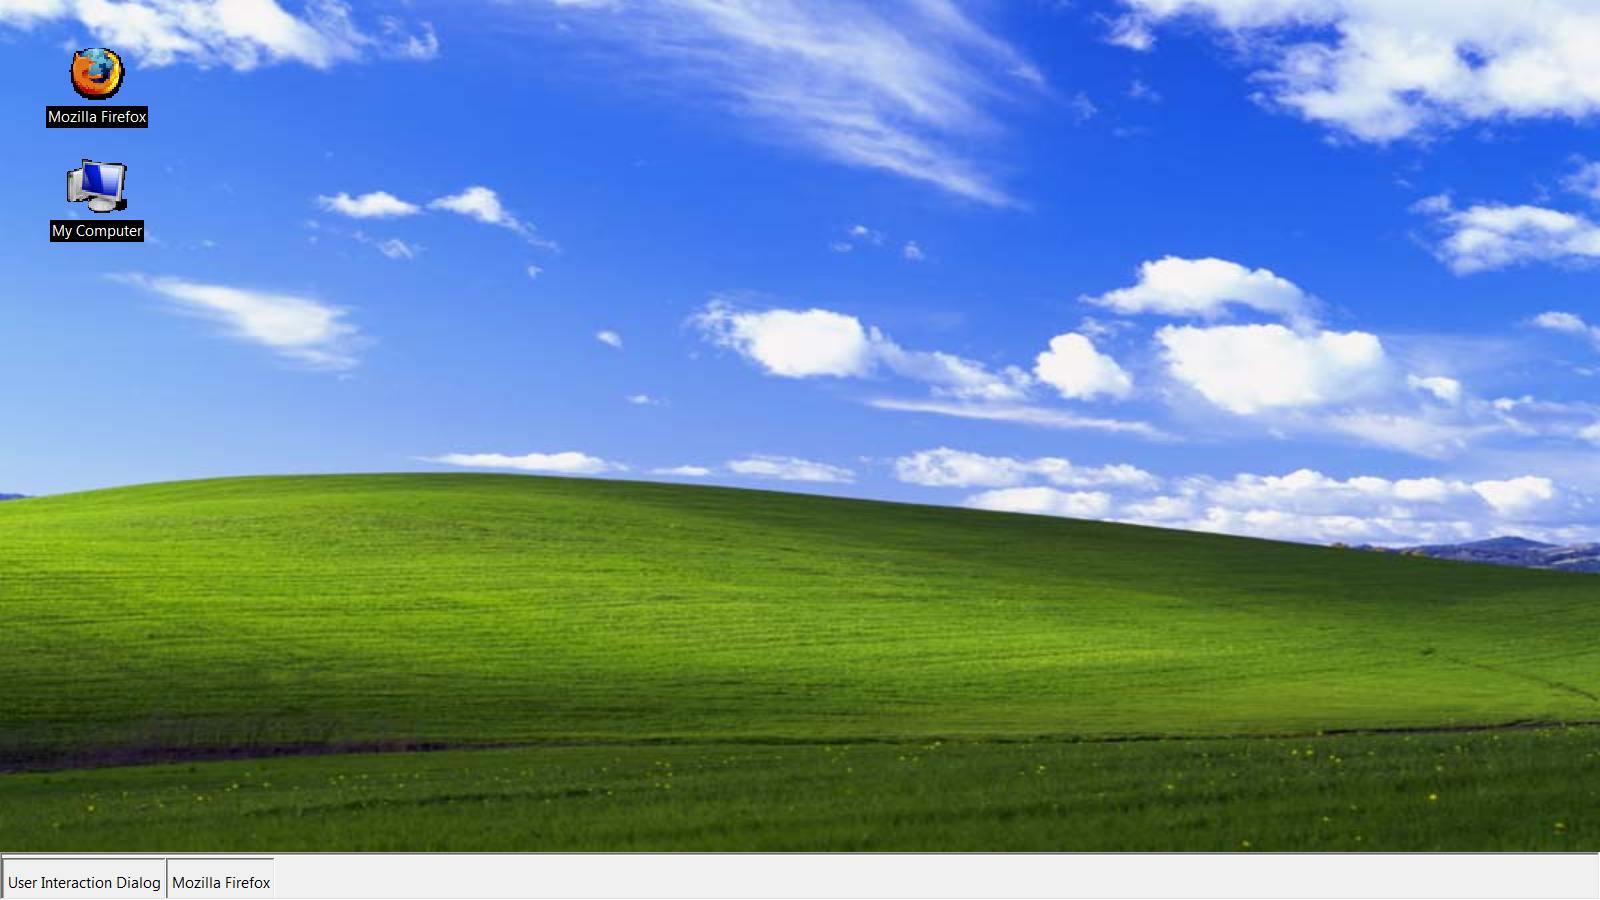
\includegraphics[width=\columnwidth]{img/desktop.png}
%  \caption{Simulated Microsoft Windows desktop environment}
%  \label{fig:desktop}
%\end{figure}
%
%In our study, the browser is the nexus; most of the interaction transpires through the browser. Subjects were instructed to open the browser which showed the starting page for the study (see
%Figure \ref{fig:browser}). The browser not only guided the subjects through the tasks of the study, but also ensured that the subjects followed the required sequences. Subjects were allowed to perform a task only when the previous task was complete. For example, installing an application could not be skipped as subjects were required to post a verification code, which they obtained after running the application.
%
%For the browser, we used FireFox (version 34.0.5) because it is open source, which allows us to customize the software to enable only the features we need for the simulated environment (forward/backward page navigation buttons, download button, address bar). To maintain the experience as being focused on computer interaction, web pages were used to collect pre and post interaction survey data. For our study, the data included demographic information as well as reports that could be compared against behavior as the subjects executed their tasks. To make the pages realistic, the URL bar in the PHP stub displayed the expected URLs (e.g., https://twitter.com) with an associated padlock to indicate that the HTTP connection was secure, when appropriate. The URL bar could be changed to test subject sensitivity to cues such as these. The browser also allowed for multiple tabs to be open for the experiment landing page and the various applications that are run within the browser.
%
%Studies on global Internet users show that checking email, sending/receiving direct messages/chat, browsing for information/research and social media activities account for the bulk of the online activities \cite{furnell2007, worldinternet2018}. Thus, simulating these activities was a priority for our tool; the current version includes simulated applications of email and Twitter. Because ``google and click'' is so open ended, we did not include it in the current version of the tool.
%
%\begin{figure}[!ht]
%  \centering
%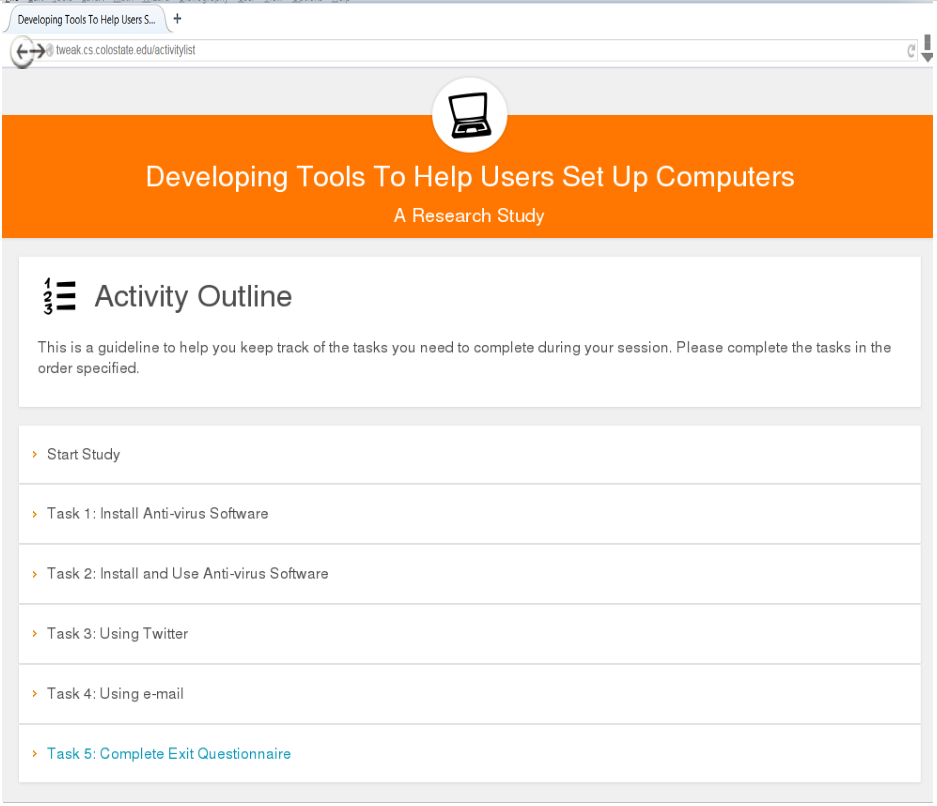
\includegraphics[width=\columnwidth, keepaspectratio=true]{img/browser.png}
%  \caption{Simulated Mozilla Firefox Web browser}
%  \label{fig:browser}
%\end{figure}
%
%Our email application was based off of SquirrellMail (version 1.4.22). SquirrelMail includes built-in PHP support for the IMAP and SMTP protocols and all pages render in pure HTML. These configurations fit perfectly to the technologies behind our simulated environment and therefore we could easily integrate it as an add-on service to the desktop environment. Our version of mail supports login and message functions. Subjects login using provided usernames and passwords and then can change their password. They can look at a list of messages, read and answer them. For purposes of this study, the email accounts can be populated with a set of email messages. Figure \ref{fig:mail} shows three emails that were used in our study and that were related to the other applications in the experiment protocol.
%\begin{figure}[!ht]
%  \centering
%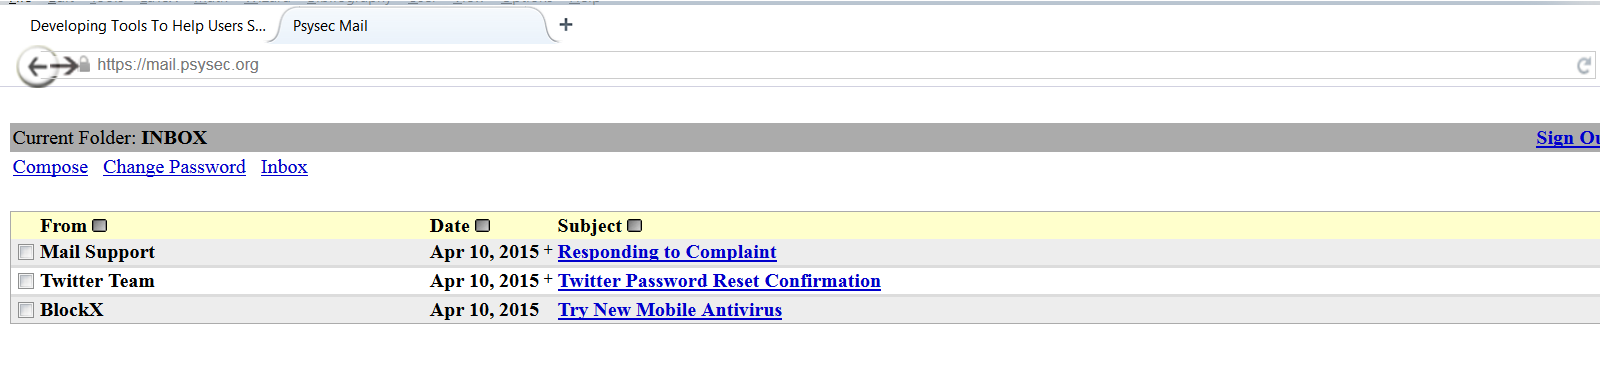
\includegraphics[width=\columnwidth, keepaspectratio=true]{img/mail.png}
%  \caption{Simulated SquirrelMail email client}
%  \label{fig:mail}
%\end{figure}
%
%As with email, our Twitter application supports login and message functions. Each participating user was provided with a twitter handle and a password. Three messages were posted in their respective Twitter inboxes (see Figure \ref{fig:twithome}). One of the three messages as shown in Figure \ref{fig:twitmsg}, which appears to link to a phishing website; if they click on the link, they are taken to a site which requested subjects to provide their Twitter username and password. 
%\begin{figure}[ht]
%  \centering
%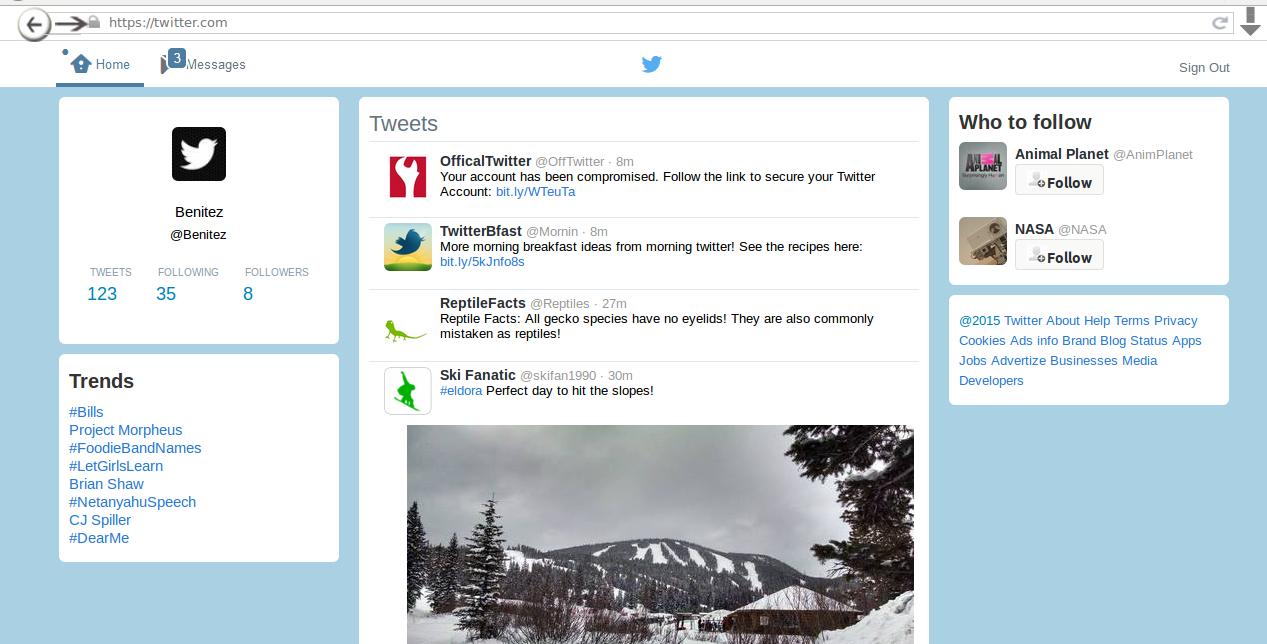
\includegraphics[width=\columnwidth, keepaspectratio=true]{img/twitterhome.png}
%  \caption{Simulated Twitter home page with three direct messages in the inbox}
%  \label{fig:twithome}
%\end{figure}
%
%\begin{figure}[ht]
%  \centering
%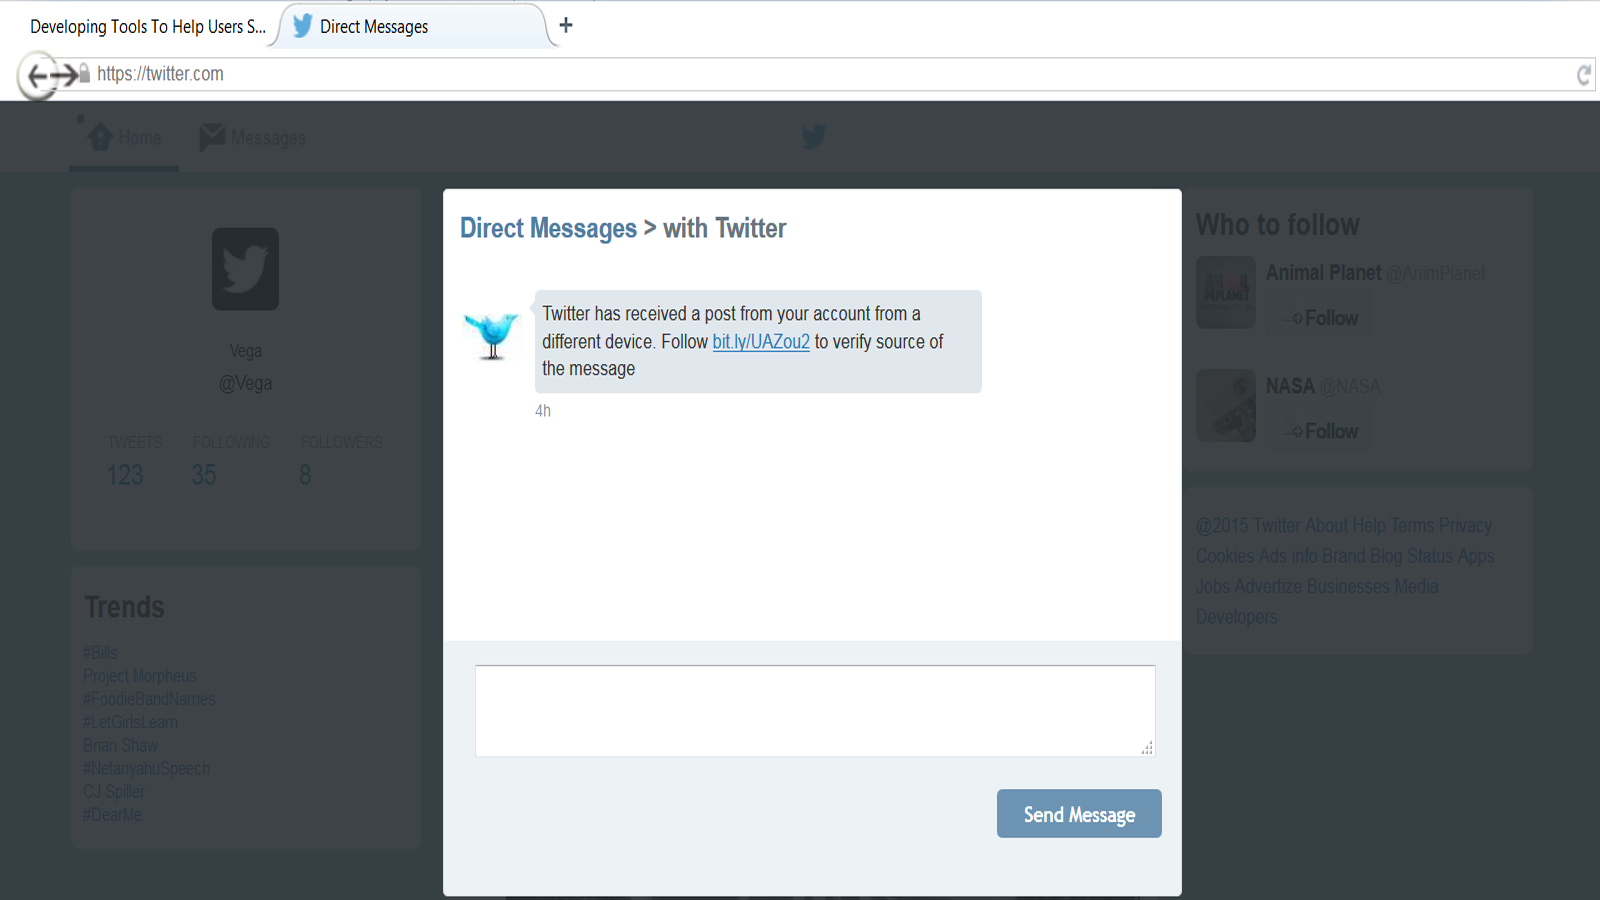
\includegraphics[width=\columnwidth, keepaspectratio=true]{img/twitter.png}
%  \caption{Simulated Twitter direct message}
%  \label{fig:twitmsg}
%\end{figure}
%
%As another activity, we included anti-virus software selection and installation. The subjects accessed an anti-virus download portal which leads to two separate websites as shown in Figure \ref{fig:virus}. One of the web-sites was purposefully made secure (HTTPS) while the other was made to look like a typical phishing site with flash images and dramatic warnings. Once the applications were downloaded, the subject was notified of the completed download. The subjects were then required to install and/or run the applications. To make sure the subjects installed and ran the downloaded application, the portal requested a verification code which was obtained by running the downloaded applications. Both anti-virus `downloads' were equipped with simulated system scanning capabilities (e.g., a progress bar appearing after the system scan is started).
%\begin{figure}[pbt]
%  \centering
%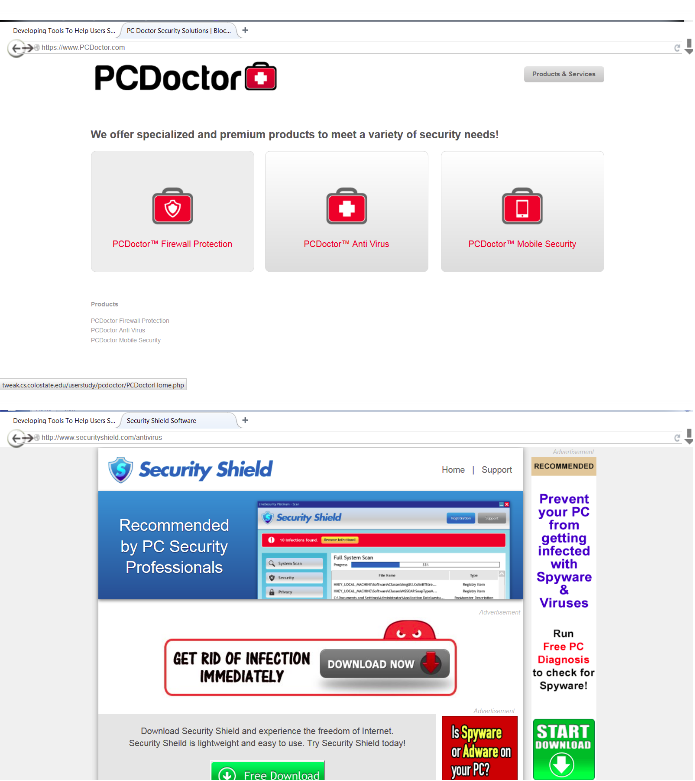
\includegraphics[width=\columnwidth, keepaspectratio=true]{img/virus.png}
%  \caption{Simulated Anti-virus download pages: secure anti-virus software (top) and unsafe anti-virus software (bottom)}
%  \label{fig:virus}
%\end{figure}
%
%
%
%\subsection*{System Architecture}
%The PsychoRithm software was designed to operate as a kiosk. The software creates a Simulated Local Environment on the subject's machine. The required applications such as the email program, the Twitter site, anti-virus software web pages, phishing web pages, and the survey questionnaires reside on the server. Software architecture diagram for PsychoRithm is shown in Figure \ref{fig:psyarch}
%\begin{figure}[pbt]
%  \centering
%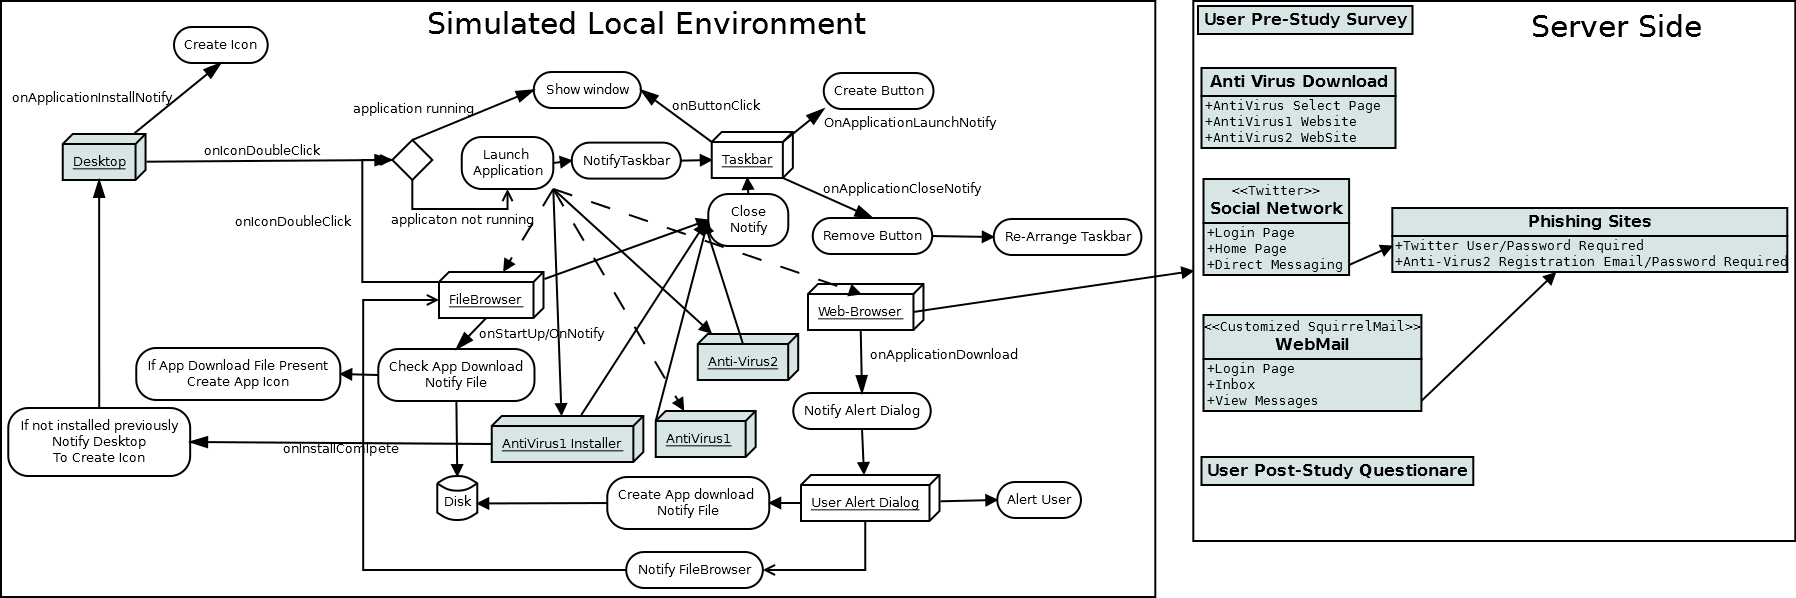
\includegraphics[width=\columnwidth, keepaspectratio=true]{img/fulluml.png}
%  \caption{PsychoRithm software architecture diagram}
%  \label{fig:psyarch}
%\end{figure}
%
%
%\subsubsection*{Desktop and File System}
%The user interacts with the desktop and the file system to download, install and run applications.
%At the start of the experiment, the user validates his experiment username with the desktop,
%and the desktop creates a folder specifically for that user. The simulated desktop provides application icons: Mozilla FireFox Web browser and the My Computer file browser (Figure \ref{fig:desktop}). The user can click these icons to run the corresponding application. When new applications are installed, such as the anti-virus software, new icons are added to the desktop. The desktop and all applications are supported by a taskbar, which provides easy access to all opened applications.
%
%To make the simulated desktop resemble a real desktop, we implemented it as the topmost Win32 Tool Window spanning the working area of the actual desktop. Underneath the simulated desktop is an invisible list-view window, which hosts the application icons. Inter-process communication was performed using custom defined messages with application specific WPARAM values. We implemented our own opaque taskbar as a Win32 Toolbar that maps a zero-based incremental index to the launched applications. This index was used to track buttons/window-handles and close/rearrange them when applications were closed.
%
%PsychoRithm was built as a package that contained empty folders like the \textit{Downloads} and \textit{LoginData}. It was placed under the \verb|C:\Users\<login_name>\Documents}| directory (to avoid conflict with system directories) and identified with \verb|login_name| on the fly to create the absolute path to the package. However, since the path was created dynamically, we could not configure the exact location of the \textit{Downloads} folder into Firefox and hence used the \textit{User Alert Dialog}. A Win32 window with an underlying list-view was used as the file browser for the \textit{Downloads} folder.
%
%
%\subsubsection*{Web Browser}
%The Web browser component allows the user to browse the content fetched from the server. To create the illusion that applications were downloaded from a specific URL, we disabled the Firefox warning dialog by editing the mimeTypes.rdf which led to Firefox calling the User Alert Dialog. Similarly, to make websites like Twitter appear to be served from twitter.com, we removed the URL bars from the existing Firefox application and introduce a custom PHP stub (enabled with Javascript navigation functions) which emulated a URL bar and allowed subjects to navigate/reload pages in same browser session. This required mocking up images that made the interface appear as expected and means that any visited URL must have a corresponding image to be loaded. Action login was facilitated by PHP session variables and AJAX event handlers.
%
%All widgets were disabled using a FireFox extension. When subjects double-clicked on the Firefox icon, the Firefox window was brought above the simulated desktop window giving the illusion that a new application has been launched. A custom designed Firefox extension allowed subjects to minimize this window, but not quit it.
%
%\subsubsection*{Email}
%The SquirrellMail portal ran on top of a DoveCot IMAP/POP3 server.
%
%\subsubsection*{Anti-virus Applications}
%Two anti-virus applications were created using Java Swing Platform. One of the anti-virus applications requires installation. After installation, it notifies the Desktop, which then creates an icon
%to launch the application. To make the download process realistic, the web browser makes a call
%to the \textit{User Alert Dialog}, which then alerts the user, creates a 0 byte file in the Downloads folder
%and notifies the file browser.
%
%\subsubsection*{Collecting Data}
%The system is instrumented to collect subject actions, specifically the start and conclusion of the session, the activation of each activity, typing and mouse clicks in the applications (buttons, widgets, windows, etc.) The results of the pre and post surveys and subject preferences (e.g., software selections, password choices) were also logged using PHP session variables. All activity related data are captured with timestamps. Once the experiment is complete, the Desktop
%process sends over all captured data to the server side using SFTP/SCP, cleans all of the local storage and kills any process that was initiated by the system.
%
%IRB regulations require us to store subject data in a safe and secure manner. Moreover, to run
%enough subjects, we needed to allow multiple subjects to participate simultaneously. Consequently,a secure remote server also stored experiment data in a safe manner. To preserve anonymity, the data were associated with the IDs (login names), which were assigned randomly when subjects arrived for the study and were never associated with specific individuals.
%
%\subsubsection*{Configuration and Extensions for Other Studies}
%
%Microsoft Windows and Visual Studio Framework are required to install and use PsychoRithm. The web applications (Twitter, Software download pages are implemented using HTML/AJAX/JQuery. The Anti-virus mock-up software is implemented using Java. For this study, the simulator only supports Web browsing (restricted only to predefined URLS), file browsing (restricted only to personalized \textit{Downloads} directory) and email (restricted only to SquirrelMail webmail application) applications. Access to other Windows applications are restricted through the simulated desktop and the web application shown in Figure \ref{fig:browser}. 
%
%Because Firefox is an existing application, it must be started at the beginning of an experiment session and cannot be stopped during the course of the experiment. As a result, the subjects were only allowed to minimize the application and restore it via the taskbar button. All menu operations, including right-click menu operations, were disabled. In this study, our main focus is on evaluating users' behavior with regard to self-efficacy and cues-to-action while performing common tasks on the computer. There are other behavior models, which describe many other factors that affect user's computer security behavior. In situ evaluations for these factors may require simulations for additional, more complected tasks. In this case, future add-on Windows applications can be developed using the aforementioned technologies and integrated as plug-ins.
%
%
%\subsection*{Studying Behavior In Situ}
%We conducted an experiment with the primary goals of:
%\begin{itemize}
% \item capturing actions taken by users when asked to perform tasks that provided ``opportunities'' to trigger security vulnerabilities
% \item characterizing their behaviors by their gender and prior experience
% \item assessing consistency in subjects answers
%and actions.
% \end{itemize}
%In this study our focus was on two factors common to several well-known models of user security behavior: self-efficacy and cues-to-action (e.g., Health Belief Model, Protection Motivation Theory). The core idea was to ask questions related to those two factors, then observe the user actions within scenarios designed to elicit potentially detrimental responses and then to ask questions about the tasks that they had undertaken. This protocol was designed to collect data on how the two factors manifest in the participant sample and to allow us to compare the self reports of against the observed actions. While we had no hypothesis about how the factors would appear, our hypothesis about the comparison of data collection methods is that self-reporting was likely to differ from observed actions. Thus, the study was designed with five parts: an introduction, a pre-study questionnaire, on-line completion of four tasks, a debriefing and a post-study questionnaire.
%
%The sandbox software allowed us to analyze participants' actual behavior when they are presented with scenarios that may lead to serious computer security exploits such as installing illegitimate software, responding to phishing email and not changing default passwords, potentially in contrast to what they report in a survey. If the participants were directly informed of the real purpose of the study (i.e., computer security practices), it is likely they would be extra cautious in completing the tasks. This self-consciousness could influence what they do in the experiment making it differ markedly from their actions outside the context of the research study (e.g., at home, workplace) and introduce an additional bias to measurements we collect. To this end, we introduced some deception into the study in three ways:
%\begin{enumerate}
%\item The description of the study used to attract participants indicated that the study was to evaluate their ability to complete common tasks on the computer so that the researchers can
%use the findings to develop tools to help users set up their computers.
%\item A task, which was unrelated to the focus of the study (i.e., compose and save email as draft)
%was added to one of the other tasks to help mask the actual purpose of the study. This task
%did not generate any useful data.
%\item To induce a sense of buy in, the participants were presented with a cover story at the start of
%the study. The cover story stated that the participant had purchased a second hand computer
%with Microsoft Windows and one utility application (Mozilla Firefox) installed. Experiment tasks were to study the participants ability to set up this newly purchased computer to be used as an additional computer by multiple users at their home. The cover story was
%communicated to participants during the introduction session.
%\end{enumerate}
%During the debriefing session, participants were informed of deception used in this study. The study was designed as a within-group experiment, where all participants were placed in identical threat scenario simulations. Written instructions were given to all participants to assist them in completing the required set of tasks. All data were collected through the PsychoRithm sandbox. Text computer logs recorded the tasks that were completed, timestamp at which a task was completed, the selections made when options were presented, external URLs visited by following links on web pages, and updates made to user visible settings. Video/audio recordings were not used. The study took approximately 45 minutes to complete.
%
%
%\subsubsection*{Participants}
%In Spring 2015, we collected data from 61 university undergraduates as participants. The students were enrolled in a psychology course during that semester. The course attracts a wide range of majors and gives research credit for participating in studies. All participants were given informed consent and participated voluntarily.
%
%Although selected as a sample of convenience, the sample was representative of home computer users from a critical group: young adults with easy access to computers. Prior studies have shown that high school and college aged adults, age between 18 and 34 report the highest level of Internet usage \cite{census2012}. 56\% of participants in this study were female. 74\% were less than 20 years of age, 25\% were aged 20-25 years and the remaining participant was aged 26-30. 98\% were working toward a Bachelor's degree.
%
%\subsubsection*{Surveys}
%We presented two surveys. The pre-study survey shown in Appendix \ref{apx:cypre} asks three questions (questions 1 - 3) about demographics and 10 questions about computer experiences (questions 4 - 13). Although we would have liked to directly assessed self-efficacy, the standard questions, as pioneered by \cite{ng2007, claar2010}, asked about level of confidence when executing specific tasks in different contexts. We did not wish to prime the participants to be thinking about computer security during the on-line portion of the study. Instead, we followed the tone of Mannan and van Oorschot \cite{mannan2008}, which asked about their experience with computers (questions 4 - 8), what challenges they perceive (question 9), where they obtain help (questions 10 - 11) and what software they have installed (questions 12 - 13). These questions were selected to relate more clearly to the cover story.
%
%For the post-study survey (Appendix \ref{apx:cypost}), we adopt the standard survey instruments, which evaluate self-efficacy for computer security practices from \cite{ng2007, compeau1995}. Instruments that measure cues-to-action are adopted from \cite{ng2007}. It must be noted that our idea of cues refer to security notifications available in the computing environment such as SSL lock icon in URLs, web site content/look and feel as opposed to external information sources like news, help-desks etc. in Ng et al.\cite{ng2007}. Questions 2 - 11 evaluate the self-efficacy of the anti-virus software usage. Questions 12 - 19 evaluate self-efficacy of safe communication over social media (Twitter). Questions 21 - 24 evaluate self-efficacy of using email and managing passwords. Questions 20, 25-29 are about awareness of secure and private information collection. Questions 30 - 35 evaluate cues-to-action on practicing computer security on the Internet. The first question asks for the pseudonym which allows us to connect the on-line portion's data with the post-survey data. The main purpose of these questions was to establish whether or not the actions in the online portion of the study corresponded to what they thought that they did.
%
%
%\subsubsection*{Experiment Procedure}
%When the participants arrived for the study, one person checked their name on an attendance list, and then another person had them pick a persona ID from folded slips of paper in a basket. The persona ID included a fictitious name, user ID and password to login to the simulated desktop. All data were collected using the persona ID, which was never connected back to the participant's actual name. They were then led to a computer and assisted in logging into the kiosk software.
%
%The starting page provided the instructions to the participants. To avoid alerting them to security issues, we presented the cover story below for what they were being asked to do.
%
%\begin{center}
%\framebox{%
%  \begin{minipage}{0.8\columnwidth}
%    \setlength{\parindent}{25pt}
%    You have just bought a second-hand desktop computer from Surplus Property, the recycle, reuse sales point of Colorado State University. This computer will be used as an additional computer at home. The computer already has Microsoft Windows operating system installed. Notepad, Windows Media Player and Mozilla Firefox web browser are installed as application software. Additionally, you also managed to get an Internet connection setup for the computer. This computer will be used by you and your family members for regular purposes such as checking email, browsing Internet, and also for entertainment activities like watching movies and videos.
%    
%  \setlength{\parindent}{25pt}
%This study helps us understand your ability to perform common tasks on a computer, while it is being set up. To familiarize yourself with the new environment, you may browse the computer and check what applications are installed. Please note that, for the purpose of this study, a custom desktop environment was created and therefore it may not have all options available in a typical desktop computer.
%\end{minipage}}
%\end{center}
%
%\vspace{1em}
%The participants were presented with a screen that described and organized their on-line tasks. This page was generated as the participant finished one activity and moved on to the next. They were first directed to take the pre-study survey. Their last task was to complete the post study survey. The online portion presented three threat scenarios: (1) selecting, installing and using an antivirus software to ensure safety of the computer, (2) communicating on social media and (3) using email.
%
%In the first scenario, participants were directed to install, configure and run anti-virus software as part of setting up their new machines. Below is the the instructions that were presented to the user as they started these tasks.
%\begin{center}
%\framebox{%
%  \begin{minipage}{0.8\columnwidth}
%  \textbf{ Task: Install Anti-virus Software}\\
%  \setlength{\hangindent}{15pt}
%	\textit{Please read the following description before you begin}
%	
%	\textit{You may have noticed that the computer does not have any anti-virus software installed. You are concerned about this lack because the computer will be shared among your family members. Your  task is to install and configure an anti-virus software to be used in this computer. Names of software you will see during tasks are fictitious.}
%
%	\begin{itemize}[topsep=8pt,itemsep=4pt, parsep=-4pt]
%	    \item \textit{On ``Study Road Map'' web page click ``Install Anti-virus Software'' Link. You will be directed to a page with two anti-virus program options: \textbf{PCDoctor}, and \textbf{Security Shield}}
%    \item \textit{Read the descriptions given for each software}
%    \item \textit{Choose ONE anti-virus program. On clicking ``Visit web page to Download Now'', you will be directed to software provider's web page.}
%    \item \textit{Find the correct download link on the provider's page. }
%    \item \textit{Click on the correct download link to automatically download the software onto your computer.}
%    \item \textit{Run installation wizard to install the software on your computer.}
%	\end{itemize}
%
%\end{minipage}}
%\end{center}
%
%Two antivirus software installations were offered via a web-based download portal implemented within PsychoRithm. One software was designed to be legitimate and safe; the other was intended as suspect and insecure. Neither were existing products or websites; in each case, we patterned our fictitious web pages after exemplars of each type of antivirus software website.  The legitimate software is ``PCDoctor'', and the suspect one is ``Security Shield''. The portal provided a brief description about each software program to assist users make a decision about which program to download. Once the software was downloaded, users were given written instructions to install the software, configure it to enable three additional security features (automatic live updates, removable media scan, and smart firewall) and finally perform a simple scanning task on the computer. Although neither program actually did anything, both were designed to give the users the interaction experience of an authentic antivirus program with appropriate timing pauses and messages (see Figure \ref{fig:rogueav}).  
%
%\begin{figure}[!pbt]
%  \centering
%  \subfloat[System scanning]{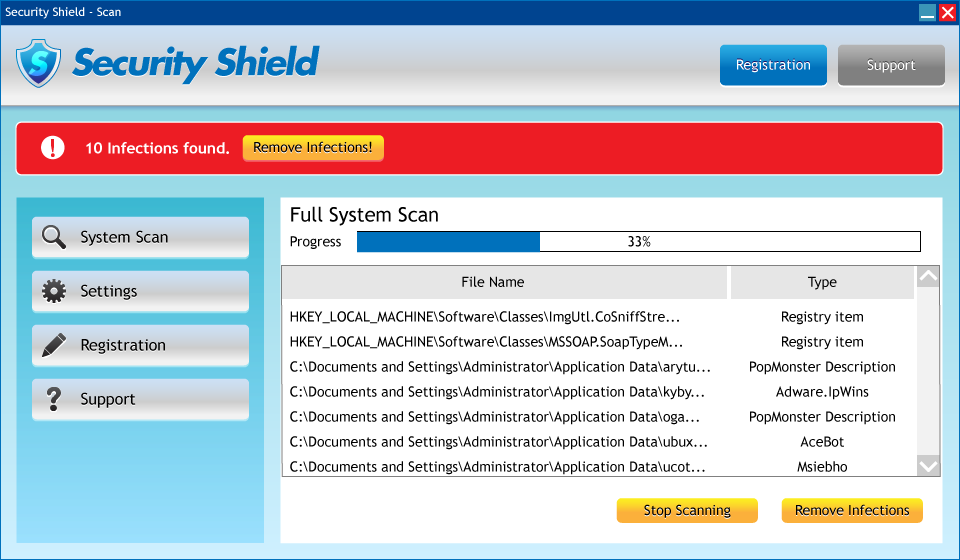
\includegraphics[width=0.5\columnwidth]{img/av1.png}\label{fig:scan}}
%  \hfill
%  \subfloat[Anti-virus protection settings]{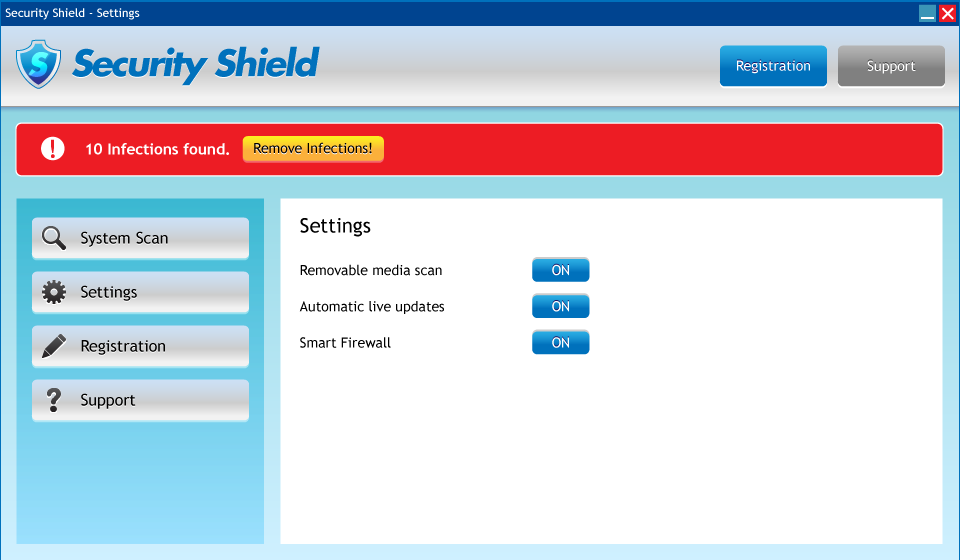
\includegraphics[width=0.5\columnwidth]{img/av2.png}\label{fig:settings}}
%  \caption{Security Shield anti-virus mock-up software}
%  \label{fig:rogueav}
%\end{figure}
%
%A mock-up version of a popular social media application (Twitter) was implemented for the purpose of studying users' communication habits. In this activity, users were instructed to use a private messaging feature of Twitter. In this case, we did create an version of the interface for the specific media site because it corresponded well with the cover story and we were interested in their behavior within this likely familiar context. Users were shown three private messages: two legitimate, safe messages sent from trustworthy sources (different offices within the university at which the study took place) and one phishing message. As shown in Figure \ref{fig:twitmsgall}, all messages contained URLs. The URL in the phishing message, directed users to a phishing website \texttt{bit.ly/UAZou2}. Once the users visited the phishing website, they were prompted to enter their username and password. In their instructions, they were told that this task would allow them to check that Twitter was working correctly on the computer; they were asked to login, read messages and ``take appropriate action''.
%
%\begin{figure}[pbt]
%  \centering
%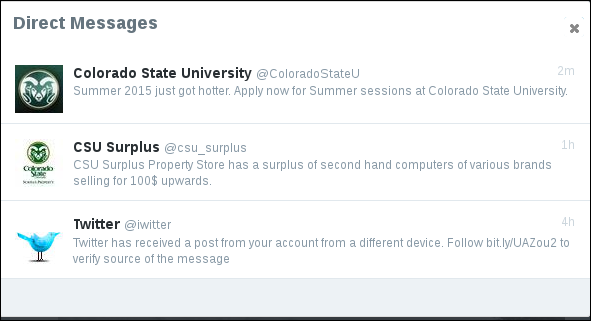
\includegraphics[width=0.7\columnwidth, keepaspectratio=true]{img/twittermsgs.png}
%  \caption{A screenshot of the messages as they appeared to the participants}
%  \label{fig:twitmsgall}
%\end{figure}
%
%A web based email client was used for the email scenario. Users were given personal email accounts and a common default password designated for the study. They were told ``The email account is unique to you. However, the default password is being shared by all users of the computer.'' The email task comprised two sub tasks. First, to study their ability to choose strong passwords, participants were instructed to change the default password of their email accounts to a new password of their choice. Second, users were instructed to compose a new email message, read email messages and respond to unread messages.
%
%As shown in Figure \ref{fig:emails}, three new messages were placed in the inbox: one safe message and two unsafe messages. One of the two unsafe messages was a phishing message with a URL that would direct the user to a phishing website upon clicking. The phishing website was masked as the web-mail client itself. The other unsafe message contained an attachment: a harmful zip file. The message content was patterned after actual phishing email messages. The phishing websites and zip file attachments were mock-ups within the sandbox; thus, they did not pose an actual security threat to the computer or to the participant's personal data. 
%\begin{figure}[htb]
%  \centering
%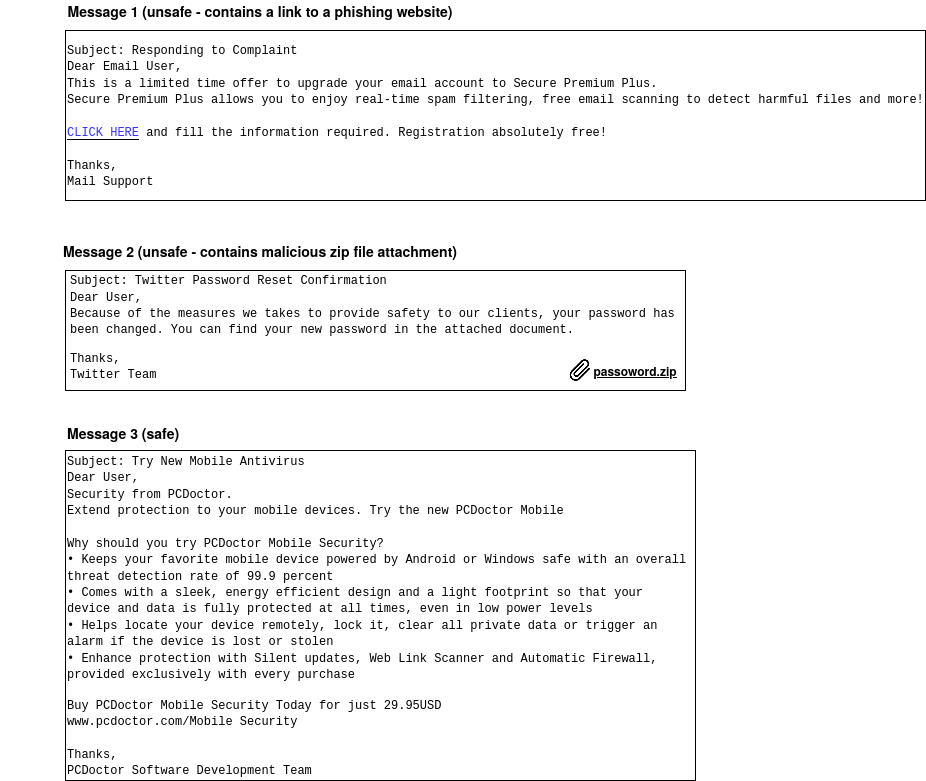
\includegraphics[width=\columnwidth, keepaspectratio=true]{img/emails.png}
%  \caption{Email messages presented as part of the online portion of the study.}
%  \label{fig:emails}
%\end{figure}
%
%We designed the phishing website to follow examples we had seen before and also placed several cues in line with commonly recognized properties of online phishing attacks \cite{ftc2019} for both the social media phishing attempt and email phishing attempt. First, in the case of Twitter, although the message sender's name was ``Twitter'', the Twitter handle (i.e., message sender's twitter account name) was not similar to the legitimate Twitter account's Twitter handle. The legitimate account's Twitter handle is \texttt{@Twitter}. The phishing message was sent from the Twitter handle \texttt{@iwitter} (i.e., Twitter misspelled). Second, the message said that some log-in attempts have been noticed. Third, the message content requested that the recipient confirm some personal information, specifically the user's Twitter account user name and password. If the user failed to recognize these cues and clicked on the link, the user is directed to a web page, which contains a log in page but looks different from the legitimate Twitter log in page. Users had already seen the legitimate log in page at the start of the Twitter task and ideally should be able to recognize that the current web page is different. We added several cues to this page as well. We changed the Twitter logo and the color scheme of the phishing web page. The URL did not contain the SSL lock icon and was \texttt{http://iwitter.com}, whereas the legitimate web site's URL was \texttt{https://twitter.com}. If the user did not recognize the phishing web site given all these cues and submitted the user name and the password, the user was directed to a landing page, which displayed a message that the user's personal information has now been compromised. Then the user was directed to the next task.
%
%A similar approach was taken to handle security attacks that occur via email. The phishing message on email was masqueraded to appear as if it was being sent by the Anti-virus software vendor. Recall that, in the sequence of tasks, when the user reaches the email task, they would have already completed the anti-virus task and is familiar with the Anti-virus vendor's name. We embedded the same discrepancies between the legitimate vendor's information and the phishing website as the Twitter phishing scenario as cues for the email phishing use case. If the user clicked the phishing link, the same sequence of events took place as in the case of the Twitter phishing scenario. There were several cues to recognize the malware email such as the generic greeting from the sender (``Dear User''), an enticement to open an attachment (get the new password by opening the attachment), information review check (password change) and undisclosed recipient (``Mail Support''). If the user clicked the attachment, the user was directed to a web page, which displayed a message that the computer system's safety is now compromised.
%
%
%Once the participant finished the tasks, he/she was directed to the post-study survey and a
%debriefing explanation. We also offered them the opportunity to further discuss the debriefing with one of the staff conducting the study.
%
%
%\subsection*{Data Analysis and Results}
%This study has two main components that evaluate users' computer security behavior: self-report surveys and the sandbox activities. Therefore, we divided the analysis as within component (only surveys and only sandbox) and across component (surveys and sandbox). We first present the analysis on single components.
%
%\subsubsection*{Pre-Survey Findings}
%Table \ref{tab:cypre} shows a summary of the pre-survey findings. Although the participants had a lot of prior experience with computers (66\% with more than 9 years), they had little formal training (59\% had none) and turned to the Internet for help as their primary source (92\%). Most (82\%) owned multiple devices. Nearly all (95\%) had installed multiple applications, i.e., Chrome, Office, Flash, Skype and Acrobat. Given the participant recruitment method, it was not surprising that nearly all had laptops and used their computers for educational activities. With respect to computer security, more than half (67\%) found it challenging to identify harmful actions and take steps to ensure safety. Yet most (77\%) had anti-virus software on their computers.
%
%\begin{table}[ht]
% \resizebox{\columnwidth}{!}{
%\begin{tabular}{|ll|}
%\hline
%Years experience &
%  4-6: 11\%, 7-9: 23\%, \textbf{\textgreater 9 : 66\% }\\ \hline
%Usage hrs/day &
%  \textless 3: 30\%,\textbf{3-6: 54\%}, 7-10: 11\%, \textgreater 10: 5\% \\ \hline
%Devices &
%  \begin{tabular}[c]{@{}l@{}}\textbf{laptops: 97\%}, smartphones 82\%, tablets: 33\%, desktop PCs: 21\%, \\ e-Readers: 7\%, Other: 3\%\end{tabular} \\ \hline
%Applications &
%  \begin{tabular}[c]{@{}l@{}}\textbf{web browser: 98\%}, Office: 82\%, Acrobat: 61\%, Media Player: 49\%, \\ Computer Games: 26\%, \\ Image Processing: 21\%, Software Development: 11\%, Other: 3\%\end{tabular} \\ \hline
%Purposes &
%  \begin{tabular}[c]{@{}l@{}}\textbf{Education: 93\%}, Documents: 84\%, Communication: 82\%, Entertainment:\\ 82\%, Information gathering: 74\%, Financial: 56\%, Work: 41\%, Games:\\ 26\%, Programming: 10\%\end{tabular} \\ \hline
%Challenges &
%  \begin{tabular}[c]{@{}l@{}}\textbf{Identifying actions that may harm the computer: 67\%}, Taking steps\\ to ensure the safety of the computer: 51\%, Installing, configuring and getting\\ a software application ready to be used: 43\%, Finding application software\\ that matches my requirements: 39\%, Finding and using help manuals: 25\%\end{tabular} \\ \hline
%Training & 
%\begin{tabular}[c]{@{}l@{}}\textbf{None: 59\%}, Application Courses: 21\%, Programming Courses: 13\%, \\ On-line Tutorials: 5\%, Face to Face Classes: 2\%\end{tabular} \\ \hline
%Help sources &
% \textbf{Internet: 92\%}, Friends: 54\%, Relatives: 46\%, Local Stores: 23\% \\ \hline
%Anti-virus usage &  \textbf{Yes: 77\%}, No: 23\% \\ \hline
%Installations &  \begin{tabular}[c]{@{}l@{}}\textbf{Google Chrome: 89\%}, Office: 85\%, Flash: 75\%, Skype: 62\%, Acrobat: 57\%, \\ Firefox: 33\%, QuickTime: 25\%, VLC Media Player: 21\%, Thirdparty email: 10\%,\\ Other: 7\%, Opensource Office: 3\%\end{tabular} \\ \hline
%\end{tabular}
%}
%\caption{Summary data from the pre-study survey questions. Each row is a question with its number and short description. Highest values in each row are in bold.}
%\label{tab:cypre}
%\end{table}
%
%
%\hspace*{-18pt}\textbf{Gender and Computer Usage Patterns} 
%
%We analyzed the data to identify any differences that may appear between male and female participants. For questions that could be coded as numbers, we ran
%two sample, two tailed T-tests. For questions that had categorical answers, we constructed $2 \times R$ contingency tables, where $R$ was the number of categories, and ran Pearson's chi-squared tests. All analyses were performed using the R statistical package. 
%
%Table \ref{tab:cypregender} shows the results for gender on questions 4, 5, 6, 7, 9 and 13. We coded years of experience (question 4) as 5 for 4 - 6 years, 8 for 7-9, and 10 for $>$ 9. We coded hours/day (question 5) as 2 for $<$ 3, 4.5 for 3 - 6, 8.5 for 7 - 10 and 11 for $>$ 10. For questions 6, 7, 9 and 13, we counted the number of answers given by each participant. Although the means on each of these questions shows some differences between female and male participants, that difference is significant for only one question: the number of challenges. The female participants reported 2.68 on average, where the male participants reported 1.70. Thus, the perception of self-efficacy in computer usage for the females was clearly lower than for males.
%
%\begin{table}[ht]
% \resizebox{\columnwidth}{!}{
%\begin{tabular}{|l|l|l|l|l|l|l|}
%\hline
%                    & Yrs Experience & Usage hrs/day & Devices & Applications & Challenges & Installations \\ \hline
%Mean Female         & 8.88           & 4.81          & 2.50    & 3.55         & 2.68       & 4.59          \\
%Mean Male           & 9.07           & 4.20          & 2.33    & 3.70         & 1.70       & 4.74          \\
%p-value \textless{} & 0.66           & 0.33          & 0.53    & 0.69         & 0.002      & 0.73          \\ \hline
%\end{tabular}
%}
%\caption{Comparing male and female participants on questions coded as numbers, Rows show mean
%for females, mean for males and p value for T-test.}
%\label{tab:cypregender}
%\end{table}
%
%Questions 6 - 13 had categorical answers. For these, we used each of the pre-specified answers as categories. We had few cases in which ``Other'' was used and so did not include that as a separate category. Table \ref{tab:cypreusage} summarizes our findings. The last column lists the category that showed the largest percentage difference and lists the percentage after the category name. For installs, no females and only 2 males installed OpenOffice, so we did not list it as the largest difference.
%
%\begin{table}[ht]
% \resizebox{0.7\columnwidth}{!}{
%\begin{tabular}{|l|l|l|l|l|}
%\hline
%Question      & \( \chi\)& df & p \textless{} & Largest Difference               \\ \hline
%Devices       & 5.58                & 4  & 0.23         & Desktop PC -21.6                 \\
%Applications  & 5.69                & 6  & 0.46         & Computer games -26.0             \\
%Purposes      & 8.44                & 8  & 0.39         & Playing games -26.0              \\
%Challenges    & 6.68                & 4  & 0.15         & Identifying harmful actions 47.5 \\
%\textbf{Training}      & 12.55               & 4  & 0.01         & No training 39.4                 \\
%Help sources  & 6.29                & 3  & 0.10         & Relatives 29.2                   \\
%\textbf{Anti-virus}    & 4.10                & 1  & 0.04         & Yes 25.3                         \\
%Installations & 9.50                & 9  & 0.39         & VLC -21.6                        \\ \hline
%\end{tabular}
%}
%\caption{Results from Pearson's Chi-Squared test on gender for questions 6 - 13. Columns show $\chi$-squared value, degrees of freedom (df), p value and the category with the largest \% difference between females and males (negative indicates lower value for females. $\alpha<0.05$}
%\label{tab:cypreusage}
%\end{table}
%
%Only two questions showed possibly significant differences due to gender in the chi-squared tests. Participants reported a considerable difference in formal training: 76.5\% females had no formal training compared to 37\% of the males. Anti-virus installation was more common for females (88.2\%) versus 62.9\% for males. One hypothesis could be that less formal training leads people to take more action with respect to security. To see whether the association might be due to the lack of formal training, we constructed a $2\times 2$ contingency table of Training (Yes/No) versus Antivirus Installation (Yes/No). A chi-squared test yielded P < 0.637 which suggests that the effect is not likely due to the lack of formal training. As a next step, we examined whether lack of formal training leads to more perceived challenges. To test this, we ran a two sample T-test on number of challenges for those with no training versus those with some training. The mean for no training was 2.47 and with some training was 1.92; the p-value from the T-test was 0.08, suggesting a marginal effect. Gender appears to exert more of an effect than training on the perception of challenges.
%
%\subsubsection*{Sandbox Findings}
%Each of the scenarios included multiple tasks. We did not use the software to force participants to complete tasks, and some of them skipped tasks. This was most true of the anti-virus installation task where 30 of the participants executed this task. For this task, 76.7\% chose the questionable anti-virus software, only 1 participant clicked on the EULA and 46.7\% of participants successfully removed all infected files.
%
%
%\begin{table}[ht]
%\begin{tabular}{|l|r|r|r|}
%\hline
%Message & \multicolumn{1}{l|}{\% Responded} & \multicolumn{1}{l|}{\% Visited Link} & \multicolumn{1}{l|}{\% Submitted Password} \\ \hline
%Safe Message 1   & 41.0 & 59.0 & N/A  \\
%Safe Message 2   & 32.8 & 57.4 & N/A  \\
%Phishing Message & 19.7 & 75.4 & 68.3 \\ \hline
%\end{tabular}
%\caption{Percentage of responding and visiting link for Twitter tasks. Also rate of submitting password for the phishing message.}
%\label{tab:twittertask}
%\end{table}
%
%For the Twitter task, the participants were asked to read and possibly respond to three messages. 61 participants preformed parts of the task. As shown in Table \ref{tab:twittertask}, participants were most likely to
%visit the phishing link and least likely to respond to the phishing message.
%
%We examined whether there was a significant difference in responding to messages, visiting links and submitting passwords between the safe and phishing messages. To do so, we constructed $2 \times 2$ chi-square tables of yes/no to action and pairs of messages as the other factor. We found significant differences in response and visiting rates (P < .0001). For the response rates, if a subject did not respond to a safe message, they were highly unlikely to respond to a phishing message (for the first safe message, 0 of 26 did so; for the second, only 1 of 40 did so); those that responded were equally likely to respond to either safe or phishing messages (13 out of 25 and 9 out of 20, respectively). For the visiting links, the relationship is still significant but the pattern is different. If the subject visited the link in the safe message, they were very likely to visit the link in the phishing message (33 out of 35 and 34 out of 24); if they did not visit the link in the safe message, they were equally likely to visit in the phishing message (14 out of 26 and 15 out of 26). The pattern of responding suggests that participants who are cautious about responding do not respond to anything; others pick randomly. The pattern of visiting suggests that participants always click links or chose randomly whether to click.
%
%The safe messages did not ask for their passwords. So we compared following the links in the safe messages to submitting passwords. Again, the relationship was significantly different (P < .0001). In both cases, if they followed a link in a safe message they were likely to submit their password; otherwise they were unlikely to submit their password.
%
%For the email task, participants were asked to change their password, compose a new email message and respond to messages. Two of the three messages were unsafe. 41 participants executed this task. As Table \ref{tab:emailtask} shows most participants did take unsafe actions in these scenarios.
%
%\begin{table}[ht]
%\begin{tabular}{|l|r|r|r|}
%\hline
%Message & \multicolumn{1}{l|}{\% Responded} & \multicolumn{1}{l|}{\% Visited Link} & \multicolumn{1}{l|}{\% Downloaded Attachment} \\ \hline
%Phishing Message & 19.7 & 73.8 & 65.6 \\
%Twitter Reset    & N/A  & N/A  & 29.3 \\
%Safe Message     & N/A  & 46.3 & N/A  \\ \hline
%\end{tabular}
%\caption{Percentage of participants responding, visiting link and downloading for Email tasks.}
%\label{tab:emailtask}
%\end{table}
%
%\subsubsection*{Post-Survey Findings}
%Tables \ref{tab:postavefficacy}, \ref{tab:posttwitefficacy}, \ref{tab:postemailefficacy}, and \ref{tab:postgenefficacy} show summaries of the post-survey answers for the Antivirus task, Twitter task, Email task and general security questions, respectively. Questions 2 - 24 and 30 are answered on a 5 point scale and are encoded from 1 to 5 (higher is better). For questions 3 - 11, 13 - 24 and 30, from Strongly Disagree to Strongly Agree. For questions 2 and 12, the answers varied from Very Hard to Very Easy. Questions 25 - 29 allowed answers of ``Yes'', ``No'' and ``I don't know''. Questions 33 and 35 allowed ``Yes'' and ``No''. Questions 31, 32, and 34 had categorical answers.
%
%\begin{table}[ht]
%\begin{tabular}{|ll|}
%\hline
%2. Difficulty with installation and configuration             & 3.623 (1.186) \\ \hline
%3. Configuration and usage                                    & 3.869 (0.939) \\ \hline
%4. Selecting software that matches requirements               & 3.623 (0.934) \\ \hline
%5. Identifying legitimate software                            & 3.525 (0.993) \\ \hline
%6. Identifying and removing suspicious files                  & 3.410 (0.990) \\ \hline
%7. Identifying and removing suspicious files without help      & 3.131 (1.126) \\ \hline
%8. Checking that download site is trustworthy                 & 3.820 (0.958) \\ \hline
%9. Choosing software that is customizable                     & 3.623 (0.879) \\ \hline
%10. Using software that is configured to preferences          & 3.492 (1.043) \\ \hline
%11. Importance of software for identifying and removing files & 4.098 (0.907) \\ \hline
%\end{tabular}
%\caption{Summary data from the post-study survey questions concerning the antivirus task. Each
%row is a question with its number and short description. Questions 3 - 7 assess confidence. Numbers are means followed by standard deviations in parenthesis. Values closer to five indicate high confidence or very easy.}
%\label{tab:postavefficacy}
%\end{table}
%
%As shown in Table \ref{tab:postavefficacy}, for the antivirus task, the highest level of confidence was in configuring and using the antivirus software. The lowest was in removing suspicious files without help, but even here, they still felt more confident than not (values greater than 3 which is neutral). Questions 6 and 7 distinguish ability with and without help. A paired sample T-test comparing the responses to questions 6 and 7 shows a significant difference (p < 0.014), which suggests that many participants were concerned about their ability to perform the task on their own. Similarly, questions 4 and 9 address different aspects of selecting antivirus software: whether the software matches requirements and whether
%it can be customized to do so. A paired sample T-test comparing the answers to the two yield
%P < 1.0 The highest variance was in how difficult it was to install and configure the software. The lowest variance was in choosing software that is customizable. However, the variances were all approximately 1.
%
%As Table \ref{tab:posttwitefficacy} shows, the participants are a little more confident in their use of Twitter than the antivirus tasks. The highest level of confidence was in responding to messages; the lowest was in checking links. Paired sample T-tests comparing the responses to questions 14 with 15 and 14 with 16 show no significant difference (P > .09).
%\begin{table}[ht]
%\begin{tabular}{|ll|}
%\hline
%12. Difficulty in responding to direct messages         & 4.361 (0.708) \\ \hline
%13. Confidence in using the direct messaging feature    & 4.311 (0.827) \\ \hline
%14. Confidence in identifying suspicious messages       & 4.115 (0.858) \\ \hline
%15. Confidence in identifying suspicious messages without help                 & 3.984 (1.025) \\ \hline
%16. Confidence in identifying suspicious messages even if it is the first time & 3.967 (0.875) \\ \hline
%17. Checking links for an unknown sender or suspicious information             & 3.918 (1.053) \\ \hline
%18. Practicing caution in following links               & 3.984 (0.904) \\ \hline
%19. Not following links if the content looks suspicious & 4.098 (0.943) \\ \hline
%\end{tabular}
%\caption{Summary data for the post-study survey questions concerning the Twitter task. Each
%row is a question with its number and short description. Numbers are means followed by standard deviations in parenthesis}
%\label{tab:posttwitefficacy}
%\end{table}
%
%As Table \ref{tab:postemailefficacy} shows, the participants are confident in their use of email. The highest level of confidence was in choosing a strong password; the lowest was in the security warnings. Paired sample T-tests comparing the responses to questions 21 with 22 shows no significant difference (P > 0.71).
%
%\begin{table}[ht]
%\begin{tabular}{|ll|}
%\hline
%20. Security warnings stop web site visits   & 3.639 (0.932) \\ \hline
%21. Practicing caution in responding to unknown senders                & 4.000 (0.913) \\ \hline
%22. Practicing caution in downloading attachments from unknown senders & 4.033 (0.856) \\ \hline
%23. Changing passwords when prompted         & 4.115 (0.819) \\ \hline
%24. Confidence in choosing a strong password & 4.213 (0.878) \\ \hline
%30. Helpful descriptions                     & 3.721 (0.933) \\ \hline
%\end{tabular}
%\caption{Summary data for the post-study survey questions concerning the Email task and 5 point
%scale Security questions. Each row is a question with its number and short description. Numbers
%are means followed by standard deviations in parenthesis}
%\label{tab:postemailefficacy}
%\end{table}
%
%Table \ref{tab:postgenefficacy}
% summarizes answers from the general security questions. Although the majority indicated they could recognize secure pages and verify secure sites, they were less sure about whether the Twitter page was secure or whether they had downloaded the antivirus software from a secure site. The cue most recognized for legitimate pages was ``HTTPS'' in the URL which suggests they have some idea of its meaning. They also were aware of the significance of an unrecognizable address in harmful email. The most common reason for not reading EULAs was they are too long.
%
%\begin{table}[ht]
%\begin{tabular}{|ll|}
%\hline
%25. Recognizing secure pages   & \textbf{Yes: 67.2}\%, No: 11.5\%, I Don't Know: 21.3\% \\ \hline
%26. Was Twitter page secure?   & \textbf{Yes: 42.6}\%, No: 26.2\%, I Don't Know: 31.1\% \\ \hline
%27. Concerned about safety     & \textbf{Yes: 77.0}\%, No: 14.8\%, I Don't Know: 8.2\%  \\ \hline
%28. Verify secure site         & \textbf{Yes: 65.6}\%, No: 23.0\%, I Don't Know: 11.5\% \\ \hline
%29. Antivirus from secure site & \textbf{Yes: 45.9}\%, No: 14.8\%, I Don't Know: 39.3\% \\ \hline
%31. Recognizing legitimate pages &
%  \begin{tabular}[c]{@{}l@{}}Appearance: 60.7\%, Contact info: 56.5\%, \textbf{HTTPS: 73.8\%},\\ Related content: 55.7\%, No ads: 54.1\%, Popular: 63.9\%, Do\\ not know: 8.2\%\end{tabular} \\ \hline
%32. Recognizing harmful email &
%  \begin{tabular}[c]{@{}l@{}}\textbf{Unrecognizble address: 86.9\%}, Unsafe links: 83.6\%, Bad\\ grammar: 70.5\%, Unpersonalized: 63.9\%, Odd attachments:\\ 72.1\%, Threats: 75.4\%, I Don't know: 0\%\end{tabular} \\ \hline
%33. Read EULA usually          & Yes: 19.7\%, \textbf{No: 80.3\%}                      \\ \hline
%34. Why not read EULA? &
%  \begin{tabular}[c]{@{}l@{}}\textbf{Too long: 47.5\%}, Too technical: 6.6\%, No harm: 4.9\%, No\\ choice: 19.7\%, Not relevant: 1.6\%, Did read it: 19.7\%\end{tabular} \\ \hline
%35. Read EULA for anti-virus   & Yes: 21.3\%, \textbf{No: 78.7\%}                      \\ \hline
%\end{tabular}
%\caption{Summary data for the categorical post-study survey questions concerning security behavior generally. Each row is a question with its number and short description. Answers are provided with percentages.}
%\label{tab:postgenefficacy}
%\end{table}
%
%
%
%\subsubsection*{Between Pre and Post Surveys Findings}
%By looking across components, we could examine 1) whether their reports of self-efficacy in the pre-survey related to their actions or their post-survey responses and 2) whether participants are consistent in their responses and actions. The pre and post surveys were designed to inquire into the participants' computer skills and perceptions of computer security and what they do generally and did within the experiment. PsychoRithm was designed to determine what they did when presented with scenarios.
%
%In the pre-survey, question 9 asked about what tasks they found most challenging. We analyzed the data to whether specific self-reported challenging tasks translated into lowered confidence in executing the tasks in the experiment. For example, did participants who reported that finding software was a challenge also have lower confidence in how they performed the antivirus task? For the analysis, we treated each task as a binary, either the participant reported it as a challenge or did not. We then ran two sample T-tests comparing those who did view it as a challenge to those who didn't for post-survey questions 2 - 7 (anti-virus), 12 - 16 (Twitter) and 24 (email). Due to the number of comparisons, we report only those with P < .01 as possibly significant differences in Table \ref{tab:prepostchallenges}.
%
%\begin{table}[ht]
%\begin{tabular}{|lll|}
%\hline
%Challenge        & \multicolumn{1}{c}{Post-survey Question}            & P     \\ \hline
%Installation     & Identifying suspicious messages in Twitter w/o help & 0.006 \\
%Using help       & Identifying legitimate antivirus software           & 0.008 \\
%Using help       & Removing files using antivirus software             & 0.009 \\
%Using help       & Removing files using antivirus software w/o help    & 0.002 \\
%Identify harmful & Removing files using antivirus software             & 0.005 \\
%Identify harmful & Removing files using antivirus software w/o help    & 0.007 \\ \hline
%\end{tabular}
%\caption{Possibly significant relationships between self-reported challenges in pre-survey and self-reported confidence in post-survey}
%\label{tab:prepostchallenges}
%\end{table}
%
%
%\subsubsection*{Between Sandbox and Post-Survey Findings}
%We now compare the users' actual sandbox activities against what they reported in the post-study survey for the three tasks: using anti-virus, communicating on Twitter and email communication. Figure \ref{fig:tasks} illustrates the task breakdown for the sandbox scenarios. Although the illustration is shown as a sequence (complies with the script that was given to the participants at the beginning of the study), we found that some participants did not follow the sequence. They skipped a sub-task to come back to it later. Other times, the participants tried the same sub-task several times.
%
%\begin{figure}[ht]
%  \centering
%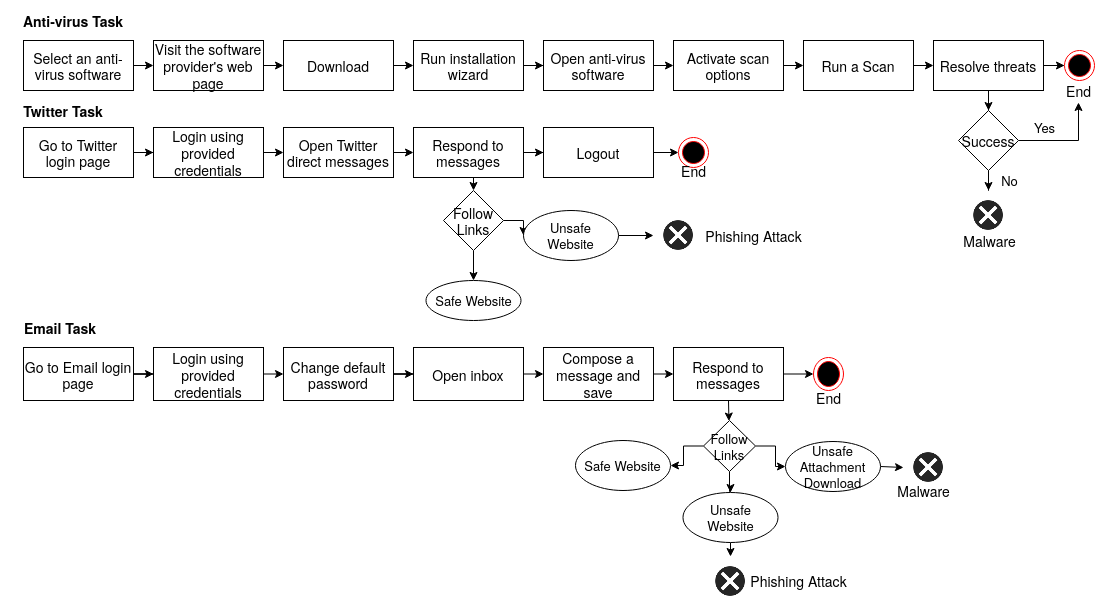
\includegraphics[width=1.1\columnwidth, keepaspectratio=true]{img/tasks.png}
%  \caption{Sandbox task breakdown}
%  \label{fig:tasks}
%\end{figure}
%
%The anti-virus task consisted of three sub-tasks: (1) given a legitimate and an illegitimate antivirus software, the user was asked to choose one (choice), (2) install the selected software and configure it to be used in the computer (install) and (3) run the software on the computer and remove threats (scan). In the post-survey, question 4 measures self-efficacy of the choice, question 9 measures the self-efficacy of the install and question 6 measures the self-efficacy of the scan. From the 62 participants only 11 completed all three sub-tasks, while 32 participants skipped the anti-virus task altogether. Those who did not complete the task skipped the install or scan or both. All 11 participants who completed all three sub-tasks installed the legitimate anti-virus software. This shows that users who practice computer security typically execute similar actions when they are placed in similar situations.
%
%Table \ref{tab:avefficacy} shows the result of the two-tailed T-test that compares the self-reported efficacy between those who completed the choice task and those who did not is significant (P > 0.05). The same can be observed for the scan activity. However, the self-reported efficacy is not significant for the install task. This shows that for certain tasks that involve anti-virus software usage, users can incorrectly assess their self-efficacy when practicing computer security in self-reports.
%
%\begin{table}[ht]
%\begin{tabular}{|l|l|l|l|}
%\hline
%Activity & \begin{tabular}[c]{@{}l@{}}Completed \\ Efficacy Mean (SD)\end{tabular} & \begin{tabular}[c]{@{}l@{}}Incomplete \\ Efficacy Mean (SD)\end{tabular} & P \\ \hline
%Choice  & 4.181 (0.603) & 2.944 (0.998) & 0.00096 \\
%Install & 3.6 (1.055)   & 3.428 (0.851) & 0.636   \\
%Scan    & 4.0 (0.707)   & 2.875 (1.147) & 0.005   \\ \hline
%\end{tabular}
%\caption{Self reported self-efficacy differences between those who completed all anti-virus sub-tasks and those who did not complete the task.}
%\label{tab:avefficacy}
%\end{table}
%
%Our post survey contained 3 questions (questions 14 - 16), which evaluated self efficacy of communicating safely on Twitter. As seen in Figure \ref{fig:tasks} the Twitter task contained the least number of steps. Furthermore, the action ``Respond to messages'' is a repetitive action. The action makes the user to read and respond to the three messages in their Twitter inbox. All 61 participants who completed the task opened/responded to at least one of the three messages.
%
%\begin{table}[ht]
%\begin{tabular}{|l|l|l|l|}
%\hline
%Question &
%  \begin{tabular}[c]{@{}l@{}}Mean (SD)\\ Visited phishing \\ link\end{tabular} &
%  \begin{tabular}[c]{@{}l@{}}Mean (SD)\\ Did not visit\\ phishing link\end{tabular} &
%  P \\ \hline
%14 & 4.31 (0.87) & 4.04 (0.85) & 0.298 \\
%15 & 4.13 (1.20) & 3.93 (0.96) & 0.571 \\
%16 & 4.31 (0.87) & 3.84 (0.85) & 0.075 \\ \hline
%\end{tabular}
%\caption{Self reported self-efficacy means (standard deviation in parenthesis) between those who visited the phishing link and did not visit the phishing link during the Twitter task}
%\label{tab:twitvisitedphishing}
%\end{table}
%Table \ref{tab:twitvisitedphishing} shows the result of the two-tailed T-test that compares the self-reported efficacy between those who visited the phishing web page following the link that appeared on their Twitter direct message and those who did not. We compute separate p-values for each question that asks the user to rate their self-efficacy. It can be seen that the participants evaluated their self efficacy to recognize phishing attempts while communicating on Twitter higher than it actually was. There is no significant difference between the self-efficacy ratings participants who clicked the phishing link and the participants who did not, P > 0.05 for all questions.
%
%\begin{table}[ht]
%\begin{tabular}{|l|l|l|l|}
%\hline
%Question & \begin{tabular}[c]{@{}l@{}}Mean (SD)\\ Visited-No Passwd\end{tabular} & \begin{tabular}[c]{@{}l@{}}Mean (SD)\\ Visited-Yes Passwd\end{tabular} & P \\ \hline
%14 & 4.25 (0.9) & 4.02 (0.85) & 0.335 \\
%15 & 4.25 (0.9) & 3.90 (0.97) & 0.316 \\
%16 & 4.25 (0.9) & 3.80 (0.84) & 0.305 \\ \hline
%\end{tabular}
%\caption{Self reported self-efficacy means (standard deviation in parenthesis) between those who visited the phishing site and did not submit their passwords and those who visited the site and submitted their passwords. P value is the two-tailed T-test}
%\label{tab:twitvisitedphishingpass}
%\end{table}
%
%A similar observation can be made for the situation where the participant visited the phishing site and submitted their password information. Table \ref{tab:twitvisitedphishingpass} shows that although there is no statistically significant difference between self reported self-efficacy ratings for the participants who visited the phishing site and also submitted their password and those visited the site but did not submit the password, those who submitted the password further compromised their security. 
%
%Users found it difficult to correctly assess their self-efficacy in practicing caution when communicating with email. Questions 21 and 22 in the post-survey asked users to rate their self efficacy. When encountered with an email containing a phishing link, two tailed T-test showed that there is no statistical significance between self-efficacy ratings given by users who did not follow the phishing link against the users who did (P > 0.05). All users, who visited the phishing link, except one submitted their login credentials to the phishing web site. The users who submitted their login credentials had a mean self-efficacy rating 3.89 (SD=0.90). Similar observation can be made from users who downloaded malicious attachments that come with email. Two tailed T-test revealed that there is no statistical significance (P > 0.05) between the self-efficacy ratings given by users who downloaded malicious attachments  from email against the users who did not.
%
%We focus on cues that are available on the computer system to evaluate how cues-to-action affect the user's computer security behavior. For the anti-virus usage task, we focused on two cues: (1) whether or not the download page was secure (has HTTPS with SSL lock icon), and (2) software provider/web page appears to be legitimate (look and feel, content etc.). Secure download was tested with post-survey question 29 and legitimate provider cue was tested with post-survey question 8. The Twitter task cues were tested with questions 17, 18, 19, 26. We considered cues such as: (1) unknown sender, (2) suspicious message content, (3)shortened URL links that appear in twitter messages and (4) secure HTTPS Twitter login page. For the email task we used two cues: (1) secure HTTPS web pages and (2) Firefox expired certificate warning. The post-survey questions 20 and 28 evaluated whether or not users picked up on these cues for email.
%
%In the anti-virus task, we used user responses to question 8 to compare self-reports of ability to recognize safety of anti-virus software by looking at the provider's web page. Participants' mean self-report value was 3.86 (SD=0.94) for the safe software and 3.00 (SD=1.00) for the unsafe software. Two tailed, T-test between the users who selected the safe software vs. the unsafe software showed that the mean difference is significant (P < 0.05). This allows us to conclude that the web page content cue helps users to select a safe anti-virus software. Question 29 had categorical responses. We used the Chi-square test of independence to determine whether the HTTPS cue is associated with users selecting a safe software. Results showed we can reject the null hypothesis that the HTTPS cue is not associated with users selecting safe software (P=0.002, df=2).
%
%In the Twitter task question 17 evaluated the unknown sender cue. Question 18 evaluated the shortened URL links in the message cue. Question 19 evaluated the suspicious message content cue. Question 26 evaluated the HTTPS with SSL padlock icon cue. Two tailed T-test for ability to recognize cues for questions 17, 18 and 19 between participants who visited the phishing link and participants who did not were not significant (P > 0.05). Question 26 contained categorical responses. We used the Chi-square test of independence to determine whether the HTTPS cues is associated with user with users following unsafe links on Twitter. Results showed we can not reject the null hypothesis that the HTTPS cue is not associated with users following unsafe links on Twitter (P=0.84, df=2).
%
%In the email task question 20 evaluated the cue of the expired certificate warning generated by the browser when following a link. Question 28 evaluated the HTTPS cue, when submitting personal information to web sites. Two tailed T-test for ability to recognize cues for questions 20 between participants who followed a link to visit an unsafe website and those who did not was not significant. Participants' mean self-report value was 3.47 (SD=0.77) for those who visited the unsafe site and 3.82 (SD=0.88) for those who did not visit the unsafe site. Question 28 contained categorical responses. We used the Chi-square test of independence to determine whether the HTTPS cues is associated with user with users submitting personal information to web sites. Results showed we can not reject the null hypothesis that the HTTPS cue is not associated with users submitting personal information to websites (P=0.85, df=2).
%
%
%\subsection*{Helping Users Avoid Danger}
%The results of our study further support the conclusions in previous studies, which states that human users' security related behavior often does not match their stated intentions \cite{davinson2010, govani2005, national2010}. PsychoRithm sandbox environment allowed us to place human users in simulated scenarios that compromised their security/privacy and record their actual responses and at the same time capture the self-reported data on how users perceive their confidence in identifying risky situations (self-efficacy) and recognize cues that indicate danger (cues-to-action). Although, we are measuring factors that affect the computer security behavior of users (extracted from the Health Belief Model), our objective in this study is not to validate the model, but rather highlight that regardless the perceived self-efficacy and availability of cues, human users can still end up compromising their security. In certain situations, if the user is not interrupted, they could end up putting their safety in even more risk. To this end, this dissertation proposal presents two models of intervention, specifically aimed at helping human users avoid undesirable consequences.
%
%In this study we mainly looked at three common home computer user tasks:
%\begin{itemize}
%\item Using anti-virus software to secure the computer
%\item Communicating with Twitter direct messages
%\item Using email
%\end{itemize}
%By analyzing the results, we identified important conditions that should be addressed when designing an intervention system to help human users. First, even though users were given step-by-step instructions for completing these task, they rarely follow the script. There were repeated as well as omitted actions. This means monitoring users to help them avoid unsafe consequences need to handle noisy and/or missing actions. Furthermore, any partially complete task (sequence of actions) that has been safe upto now may quickly turn unsafe. This means that the intervention decisions need to be made online (as and when actions are observed). Users perform a large number of actions; while few of them incur much risk, some are pivotal in triggering vulnerabilities. For example, from our using email task, opening email action itself is not a risky action. However, when the email is from an unknown sender and contains suspicious attachments, preconditions to a malware vulnerability have manifested within the system. In this state, the opening email, although a normal action for a human user, is actually high risk action.
%
%Second, we need to evaluate two objectives: \textit{undesirable consequences} and \textit{user intention}. Undesirable consequences  assesses whether an action is likely to lead to undesirable outcome (e.g., security breach), immediately or as part of an action sequence, or may provide conditions that an attacker can exploit. User intentions determines what the user is intending to do through his/her actions, the short or long term goals (e.g., send an email to a friend). User's do not intentionally trigger the security breaches. Rather, the breach occurs as a result of the user being unaware of some risk that exists in the computer system. Thus we need a model of actions (user actions and system actions), which describes how vulnerabilities can manifest in the computer system. By comparing the monitored user actions and system state to the model and evaluating them for the two objectives, it will be possible to recognize pivotal actions.
%
%
%Third, the cyber-security domain typically contains an attacker and a user, who function in an adversarial role. In our study we did not explicitly model an attacker. However, effects of the attacker's actions (e.g., phishing message, malicious attachment) are present in the computer system. We think this is a fair assumption because, in most of the cyber threats, the attacker is not physically present in the domain. Instead, the attacker will execute the attack remotely and we will only see the effects of the attack in our domain. Finally, the study generated actual action traces, which we can use to evaluate undesirable consequence recognition algorithms.
%




%The cues-to-action we have discussed in this study are preconditions that exist in the computer system. For example, if we had a background process in the computer system monitoring system state, it should be able to identify whether the web page the user is visiting contains the HTTPS SSL padlock icon, or whether the user is opening an email sent by an unknown (not in address book) sender.
% when is the best time to intervene?
%certain actions in a sequence has more criticality than others
%there are common action sequences for good plans and bad plans
%
%cues are mostly like preconditions that already exist in the environment
%efficacy is like related to actions users execute



%%%%%%%%%%%%%%%%%%%%%%%%%%%%%%%%%%%%%%%%%%%%%%%%%%%%%%%%%%%%%%%%
%\chapter{Predicting Undesirable Consequences Before they Happen}
%\label{chap:ranking}
%\section*{Introduction}
%A wealth of literature in plan and goal recognition has examined how to infer a single agent's plan \cite{GeibGoldman09, ramirez2009plan}, the agent's goal \cite{ramirez2011goalrecog, yin2004high}, or the goals or plans of multiple agents \cite{banerjee2010mpr, kaminka2002monitoring}. Some recent work has even examined plan/goal recognition in the face of noisy observations \cite{geib2005partial, vattam2015case} or extraneous actions \cite{gal2012plan, sohrabi2016finding}. Yet relatively little of this research considers the question of when to intervene if one wants to thwart the plan or goal if, for example, the agent we want to disrupt is at the risk of producing an undesirable state. The decision of when to intervene must be made judicially. Intervening too early may lead to wasted effort chasing down false positives, helpful warnings being ignored as a nuisances, or leaking in formation for the next attack. On the other hand, intervening too late may result in undesirable consequences.
%
%Our motivating application is a software agent that monitors the state of a personal computer to help home computer users avoid security and privacy vulnerabilities. Home computer users are viewed as the ``weakest link'' in computer security because they lack the time, knowledge and resources to defend against the increasing inciddents of computer security and privacy threats \cite{sasse2001transforming}. Moreover, some threats, such as software downloads and phishing, require user action or at least acquiescence \cite{howe2012psychology}. Security analysis for home computer users focuses on identifying threats on a personal computer by modeling attacker actions, the system state of the computer and computer user's actions, including both ordinary and risky actions. The Personalized Attack Graph (PAG) extends the attack graph model \cite{Sheyner2002} to support individual computer/user level granularity and by representing the states and actions in PDDL \cite{urbanska2013}. Attacker actions do not include actions that cannot be observed on the home computer. System states can include levels of partial compromise (e.g., access to the password key-chain), configuration information (e.g., operating system), and state changes achieved on specific system components (e.g., implanting a keystroke logger).
%
%In this work, we examine how well an algorithm can determine the best intervention point for the cyber-security application, calling it a ``\textit{critical trigger action}'' because it may lead to undesirable state. As each situation may have a unique definition of the ideal intervention point, we formulate intervention as a combination of three domain independent metrics: (1) \textbf{timeliness}, which quantifies how soon the undesirable state may occur, (2) \textbf{certainty}, which highlights frequently occurring actions as important, and (3) \textbf{desirability}, which measures the contribution of the action to user's own objective. The desirability metric helps separate common harmless actions that further the user's actual goal from harmful actions to be avoided. A critical trigger action is a user action that maximizes the linear combination of these three metrics.
%
%Given a PDDL domain model, a set of undesirable states to avoid, and an observation trace of actions, our algorithm identifies critical trigger actions. An intervention is correct if, compared to a ground truth trace, the algorithm (1) ignores extraneous actions (i.e., as true-negatives) and, (2)
%identifies actions leading to undesirable state (i.e., as true-positives). We begin with a study of traces taken from a human subject study for computer security. We then generalize our results to four benchmark planning domains and
%consider the impact of missing and extraneous observations of actions and test the algorithm. Across all benchmark domains, certainty and desirability metrics perform well in ignoring extraneous actions, while the timeliness metric and
%it's combinations with certainty and desirability perform well in identifying true positives. Thus, in this work we have identified two metrics that are sensitive to noise in action based observation traces and a metric that is sensitive to partial observability of actions.
%
%\section*{Related Work}
%The two most closely related areas of literature are plan recognition and automated planning for cybersecurity. Plan recognition is the problem of inferring the course of action (i.e., plan) an actor may take towards achieving a goal from a sequence of observations \cite{schmidt1978plan,kautz1986generalized}. The constructed plan, if followed to completion, is expected to result in states that correspond to goals of the actor, which in turn presupposes that the actor intends to achieve those goals. Many approaches to plan recognition use a plan library to infer a relationship between the observed actions and hypothetical plans/goals \cite{carberry2001plan}. For example, PHATT enumerated all plans, which included the observations, to compute the proportion consistent with each goal \cite{GeibGoldman09}. Plan libraries use pre-compiled plans (with some approaches allowing for learning new plans \cite{lesh1996,bauer1998acquisition}), which can limit the set of recognizable sequences. Our objective in undesirable consequence recognition is different to the plan/goal recognition problem because we assume that the user's goal is not known and the user does not want to intentionally trigger the undesirable state.
%
%Hong \shortcite{hong2001goal} constructed a ``Goal Graph'' of observed actions, world state nodes and goal nodes; this graph  was analyzed to extract the goals that explained the observed actions. Sun and Yin \shortcite{sun2007recognizing} constructed valid plans given a partial set of observations extending the Planning Graph \cite{blum1997fast} to allow for states to be unknown and embedded the analysis in a system that incrementally updated the graph while action transpired. Ramirez and Geffner \shortcite{ramirez2009plan,ramirez2010probabilistic} used an existing planner to generate hypotheses from observations. Their approaches offer advantages of being more adaptive to input as well as exploiting existing planning systems and plan representations. Their first approach computed the set of goals that can be achieved by optimal plans that match the observations. Their second approach removed the optimality constraint and computed a probability distribution across possible plans that could be generated from existing planners. Vattam et al. \shortcite{vattam2015error} allowed for missing or misclassified actions in the traces. Their SET-PR represented library plans as action sequences and computed a similarity metric between observations and known plans. To recognize actions that may lead to undesirable states, we propose a variant on plan recognition, which incorporates the attacker/system, and exploits the granularity and power of an existing planners.
%
%
%AI Planning has previously been used to reason about computer security.  Boddy et al.~\shortcite{boddy2005course} built Behavioral Adversary Modeling System, which could identify potential vulnerabilities and countermeasures with a focus on insider subversion. Sohrabi et al.~\shortcite{sohrabi2013hypothesis} generated hypotheses of which nodes in a network might be infected with malware. The Core Security model captures the actions of attackers at the level of known network vulnerabilities\cite{lucangeli2010attack}. Hoffmann has  extended the Core Security model as a POMDP \cite{hoffmann15} for penetration testing: simulating what an attacker might reasonably try over time. Geib and Goldman \shortcite{GeibGoldman09} defined a domain in which attackers try to achieve one of three goals: \emph{Bragging}, which is the attacker boasting of success, \emph{Theft}, which is the theft of information, or causing a \emph{Denial of Service} to legitimate users by exploiting security vulnerabilities on servers.  
%
%The CIRCA architecture for adaptive real-time control systems \cite{goldman1997} presents a solution to the problem of avoiding undesirable states. They proposed the concept ``temporal preemption'', which builds event controllers (plans) that make potential failure states unreachable, and thereby keeping the system safe. The difference between their domain and ours is that in their domain, the actions to which the plans are generated have timing constraints/durations and ours do not. Further, our focus is on identifying the intervention point as early as \textit{helpful} when a user may be triggering an undesirable state.  Our proposed algorithm works incrementally. As a user action is detected, a planning problem is constructed in which the initial state is the current state of the system and the goal state is the set of known vulnerabilities OR’ed together. We build a tool set that monitors the computer system state and provide the necessary observation traces and system state information for the planner to sample the plan space to find plans that can lead to one or more vulnerabilities and help identify actions that lead to triggering the vulnerabilities.
%
%
%
%\section*{Intervention in Cyber-security Domain}
%\subsection*{Example}
%Before introducing a formal definition, we present an example to clarify the key concepts. Suppose a user wants to read email (e.g., the goal $G$) but there exists an undesirable state $U_1$ (e.g., \texttt{installation of malicious software}). Figure~\ref{fig:cybersecproblem} illustrates the \emph{possible} manifestation of $U_1$. The user has executed actions $a1, a2, \ldots$ (e.g., \texttt{start email application, log in to email account}) from the initial state $I$ to achieve  $G$, resulting in post conditions $S_{a1}, S_{a2}, \ldots$ 
%
%Let us now consider possible plans that lead to $U_1$ through actions $b, c, d, f, g, h, j, k, l, m, n, p, q$. In the context of email, these actions might be clicking phishing links, downloading affected files, etc. We will call these \emph{undesirable plans} and denote any such plan as $\pi_{U_1}$.
%Ideally, the user would continue toward achieving $G$. However, by mistake or undue influence, the user may deviate from pursuing $G$ and unwittingly follow paths reaching $U_1$. The intervening agent has observed the action sequence $O$ = $\{a1, a2, a3\}$ user has executed. In state $S_{a3}$, the user might reach $U_1$ through a set of undesirable plans $\Pi_{U_1}=\{(bgn[u_1]), (bgmq[u_1]), (ch[u_1]), (cjp[u_1]), (cjdfl[u_1]),(cjdfkp[u_1]), \\(fl[u_1]), (fkp[u_1]),(fkdfl[u_1]), (fkdfkp[u_1])\}$ where a plan is a sequence of actions (letters) followed in brackets by the undesirable state that results and each letter ($b, c, d, f, g, h, j, k, l, m, n, p, q$) denotes candidate trigger actions (an action that appears in at least one undesirable plan). Our question is: \textit{given the current state $S_{a3}$, which action in the set of actions in $\Pi_{U_1}$ will be the best action for the security agent to intervene if observed?}
%\begin{figure}[pbt]
%	\centering{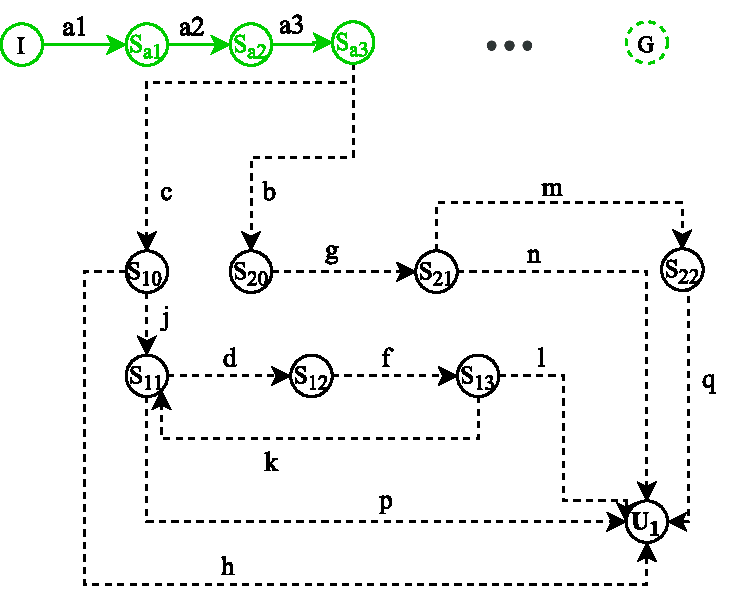
\includegraphics[width=0.5\columnwidth]{img/cybersecexample.pdf}}
%	\caption{An application domain where a user executes actions $a1, a2, \ldots $ in succession to transform initial state $I$ to a goal state $G$. An undesirable state $U_1$ may develop from state $S_{a3}$ after $a3$ has been executed, following dotted paths towards $U_1$.}
%\label{fig:cybersecproblem}
%\end{figure}
%
%\subsection*{The Intervention Problem}
%We adapt the notation used by Ramirez and Geffner \cite{ramirez2010probabilistic} to define the intervention problem.  First, we define the cyber-security domain as a planning problem using STRIPS \cite{fikes1971strips}, which defines the problem as a state transition system. In the STRIPS language, state variables have the domain $\lbrace True, False\rbrace$ and an operator consists of two sets of state variables \textbf{preconditions} and \textbf{effects}. Preconditions are state variables that needs
%to be True for the operator to execute. Effects are state variables that will be True (and False) as a result of the operator executing.
%
%
%\begin{definition}
%A STRIPS planning domain is a tuple $\mathcal{D}=\langle F, Op\rangle$, where $F$ is a finite set of  state variables (predicates) and $Op$ is the set of operator schema. An operator schema $op \in Op$ is a tuple $ op = \langle Pre(op), Add(op), Del(op)\rangle$ that consists of preconditions, add and delete effects respectively, where $Pre(op)$, $Add(op)$, $Del(op)$ are all subsets of $F$. Predicates and operator schema have parameter lists and can be instantiated with objects (defined later). An instantiated operator (action) $op$ is applicable in a state $s$ if predicates in $Pre(op)$ are \textit{True} in $s$. A state transition induced by an action $op$ in a state $s$ is defined as a function $\delta$:
%\begin{equation*}
%\delta (s,op) = \left\{\begin{matrix}
%s\setminus Del(op) \cup Add(op) & Pre(op) \subseteq s\\ 
%undefined & otherwise
%\end{matrix}\right.
%\end{equation*}
%\end{definition}
%
%\begin{definition}
%A STRIPS planning problem is a tuple $P = \langle \mathcal{O}, I, G\rangle$, where $\mathcal{O}$ is the set of objects. Objects can be either constant or non-constant and may have a type. Constant objects are common to all instances of the domain definition and shared by planning problems defined on that specific planning domain. Non-constant objects are unique to a specific planning problem. $I \subseteq F$ is the set of propositions that are true in the initial state, $G\subseteq F$ represents the goal specification.
%\end{definition}
%
%Given a domain $\mathcal{D}$ and a planning problem $P$, an automated planner generates the planning task $\Pi=\langle \mathcal{F}, \mathcal{A}, I, G\rangle$, where $\mathcal{F}$ is a finite set of grounded propositions, $\mathcal{A}$ is the finite set of grounded actions instantiated from the operator schemata $Op$, $I$ is the grounded propositions specifying the initial state and $G$ is the grounded goal specification. Objects in $\mathcal{O}$ are used to ground $\mathcal{F}$, $\mathcal{A}$, $I$ and $G$. Grounding replaces the variable terms in the parameter lists of the propositions, action schema, goal specifications with constant/non-constant objects. 
%
%\begin{definition}
%A solution to $\Pi$ is a plan $\pi=\lbrace a_1, \ldots, a_k\rbrace$ of length $k$ that modifies $I$ into $G$ by successive execution of actions  $a_1, \ldots, a_k$ 
%\end{definition}
%
%We defined a domain model for the cyber-security domain using PDDL (Planning Domain Definition Language) a generalization of STRIPS, shown in Figure \ref{fig:cybersecdomain}. In total this domain model has 45 actions, 47 types, 70 constants and 55 predicates.
%
%\begin{figure}[pbt]
%\noindent\fbox{
% \parbox{\textwidth}{\raggedright: 
%{\small
%\texttt{(define (domain attackgraph-typed)}\\
%\texttt{\hspace*{35pt}(:requirements :strips :adl :equality :typing \hspace*{35pt} :disjunctive-preconditions)}\\
%        \hspace*{35pt}\texttt{(:types unknown software misc - object)\\
%       \hspace*{35pt} \texttt{account certificate email-ID file key site user attacker vulnerability-type password direct-message device database parameter permission process username response request - misc}\\
%\hspace*{35pt} \texttt{browser editor webmailer plug-in site-creating-software server-connecting-software server anti-virus OS desktop-app server-app malicious-software - software}\\
%\hspace*{35pt} \texttt{phishing-site server-site normal-site - site}\\
%\hspace*{35pt} \texttt{phishing-site-email phishing-site-twitter - phishing-site}\\
%\hspace*{35pt} \texttt{attacker-remote attacker-local - attacker)}
%        }\\ [15 pt]
%\hspace*{35pt}\texttt{(:constants \\ 
%\hspace*{35pt}user1-email-account user1-twitter-account - account \\
%\hspace*{35pt}pc-doctor security-shield - anti-virus \\
%\hspace*{35pt}browser-firefox - browser \\        \hspace*{35pt}phishing-direct-message - direct-message \\
%\hspace*{35pt}email-with-malicious-attachment - email-ID\\
%\hspace*{35pt}squirrelmail - webmailer\\
%\hspace*{35pt}user1-twitter-password - password $\ldots$ )\\[15 pt]
%}
%\hspace*{35pt}\texttt{(:predicates \\
%\hspace*{35pt}(information-available ?aUser - User ?anAccount - account) \\
%\hspace*{35pt}(user-has-email-account ?anAccount - account)\\
%\hspace*{35pt}(direct-message-received ?dmsg - direct-message)\\
%\hspace*{35pt}(anti-virus-software-selected ?av - anti-virus) \\
%\hspace*{35pt}(information-leakage ?anAccount - account $\ldots$ )\\[15pt]
%}
%
%\hspace*{35pt}(\texttt{:action user-visit-antivirus-download-site}\\
%\hspace*{35pt}\texttt{:parameters (?U - user ?aBrowser - browser ?aSite - site \\\hspace*{35pt} ?av - anti-virus)}\\
%\hspace*{35pt}\texttt{:precondition ( and (logged-onto-system ?U) \\\hspace*{35pt} (use-software ?aBrowser) (running ?aBrowser) \\\hspace*{35pt} (= ?aSite antivirus-software-download-site) \\\hspace*{35pt} (not (installed ?av))  (not (running ?av)) )}\\
%\hspace*{35pt}\texttt{:effect (and (user-visits-site ?U ?aSite))}
%)\\[15pt]
%
%\hspace*{35pt}\texttt{(:action user-opens-attachment-through-webmail}\\
%\hspace*{35pt}\texttt{:parameters (?U - user ?aBrowser - browser ?WM - webmailer \\\hspace*{35pt}?aSite - site  ?anAccount - account ?Msg - email-ID  ?F - file )}
%\hspace*{35pt}\texttt{:precondition (and  (use-software ?aBrowser) (running ?aBrowser) \\\hspace*{35pt}(user-visits-site ?U ?aSite) (= ?aSite webmail-site)\\\hspace*{35pt}(user-has-email-account ?anAccount)\\\hspace*{35pt}(= ?anAccount user1-email-account) (msg-opened ?Msg)\\\hspace*{35pt}(mail-attachment ?Msg ?F) (logged-onto-system ?U))}\\
%\hspace*{35pt}\texttt{:effect (opened ?F))} 
% )\\\hspace*{35pt}$\ldots\ldots$
%}
%}
%}
%\caption{The cyber-security PDDL domain model snippet}
%\label{fig:cybersecdomain}
%\end{figure}
%
%\begin{definition}
%An observation trace $O$ is a sequence of observed actions $O = \{o_1, o_2, ... ,o_n\}  \;where\; o_i\in \mathcal{A}\; and \; i=1,2, \dots ,n\; (n = $ length of observation trace) and states resulting from execution of actions $o_i\in O$ are known. 
%\end{definition}
%
%Traces may contain extraneous or missing actions.  An \emph{extraneous action} is an observation $o \in O$ such that the state resulting from executing $o$ is never added to the state (i.e., set of state variable predicates that are true) by any of the actions $a_i \in \pi_U$. A \emph{missing observation} with respect to $\pi_U$ occurs when the state resulting from executing $o$ is added to the global state by an of the actions $a_i \in \pi_U$, and $o \notin O$.
%
%When we are looking for possible paths leading to undesirable state, we search for a \textbf{undesirable plan} $\pi_U = \{a_1, \dots ,a_k\}$ of length $k$ that entails the one or more undesirable states $U\subseteq \mathcal{F}$ and $a_i \in A$. There may be more than one undesirable plan, in which case we consider a set of undesirable plans $\Pi_U$. In the example in Figure \ref{fig:cybersecproblem}, the domain has only one undesirable state $U=\lbrace U_1\rbrace$.
%
%
%\begin{definition}
%An intervention problem $T = \langle \mathcal{D}, O, I, U \rangle$ consists of a planning domain $D$, a sequence of observed actions  $O \subseteq \mathcal{A}$, an initial state $I \subseteq \mathcal{F}$, a set of undesirable states $U\subseteq \mathcal{F}$.
%\end{definition}
%The solution to the intervention problem is a binary decision for each action in the observation trace, $o \in O;  o \rightarrow \lbrace Yes, No \rbrace$ indicating whether it was identified as a critical trigger action ($Yes$) or not ($No$).
%
%\subsection*{Identifying Critical Trigger Actions}
%A \textbf{critical trigger action} $c_i$ is a  action at $o_i \in O, i\leq |O|$ that maximizes the metric function $V (c_i)$, which we define now.
%
%We recognize two forms of candidate trigger actions in the observation trace: strong and weak. A strong trigger can actively contribute to causing the state (e.g., as an effect or by satisfying a required precondition) or allow another actor to cause it. A trigger may also weakly contribute to the causation of the undesirable state(s) and may not be worth intervening to prevent. Consequently, we add a layer to the intervention problem to support application specific ranking about which actions are most ``critical'', i.e., helpful in preventing the undesirable state(s). The key addition is an objective function that allows a tunable combination of metrics.
%
%Our focus is on identifying the intervention point as early as  \textit{helpful} when a user may be triggering an undesirable state. The concept of helpful is similar to the value of alerts described in \cite{Wilkins2003} which recognized that it is important to be judicious in interrupting a user in scenarios where humans and machine agents interact with each other: don't ignore but don't annoy. To this end, we start by defining a function composed of three  metrics to quantify the notion of helpfulness: \textbf{certainty}, \textbf{timeliness} and \textbf{desirability}. These metrics are calculated based on a set $\Pi_U$.
%
%
%When producing the set of alternative undesirable plans $\Pi_u$, as representative of a set of possible trajectories toward an undesirable goal, it would be best to consider alternatives that are non-obvious and diverse from each other rather than just the optimal plan.  This is especially important in long-running processes with complex traces or when a sub optimal plan contains a longer, but perhaps more easy to trigger, path to the undesirable state.
%
%{\it Certainty} measures the likelihood of action $a$ occurring in $\Pi_U$.
%\begin{equation}
%\label{eq:certainty}
%Certainty (a|\Pi_U)  = \frac{|\pi_U \in \Pi_U \textup{ in which}\; a\; \textup{occurs}|}{|\Pi_U|}
%\end{equation}
%Actions occurring frequently in $\Pi_U$ indicate the importance of that action toward causing $U$. For example, if an action $a$ occurs in all plans $\Pi_U$, the certainty metric will assign a high value to $a$, giving it a higher probability of being selected as a critical trigger compared to a less frequent action. 
%
%{\it Timeliness} requires knowing what actions could yet be observed, which might effect the causation of the undesirable state. For this study, timeliness is measured by the maximum normalized steps remaining in $\Pi_U$ in which the action a occurs. Timeliness quantifies how soon an observation will trigger the undesirable state. Therefore, we compute the maximum in discrete time as opposed to the minimum because it indicate that an undesirable state is developing but not imminent and allows time to recover. Let $n$ be the remaining number of steps in $\pi_U \in \Pi_U$ after some action $a$. Then,
%\begin{equation}
%\label{eq:timeliness}
%Timeliness (a|\Pi_U) = \max_{\pi_U \in \Pi_U}\left(\frac{
%	\max\left( n \right)\
%	}{\; |\pi_U|}\right) 
%\end{equation}
%
%{\it Desirability} measures the effect of an action on user's goals, which is ignored in the other two metrics. It separates common harmless actions (e.g., user opening web browser) from avoidable ones and connects the observations to knowledge of the user's goals. In this study, we use {\it Desirability}
%to downgrade the contribution of common actions to criticality. Hence, the negative metric:
%\begin{equation}
%\label{eq:desirability}
%Desirability (a|\Pi_U) = - \frac{|\textup{appearance of}\; a\; \textup{ in } \Pi_U|}{\sum_{i=1}^{|\Pi_U|}\left | \pi_i \right |}
%\end{equation}
%
%Together, these metrics define the function $V(a)$ for candidate trigger action $a$ for a weighting provided by $\alpha$, where $\alpha$ $=\lbrack\alpha_1, \ldots, \alpha_m \rbrack$, $\alpha_i$ is in the range $\lbrack0,1\rbrack$, $m$ is the number of objectives and $\sum_{1}^{m}\alpha_i = 1$:
%
%\begin{equation}
%\label{eq:function}
%V(a) = (\alpha_1 \times Certainty (a|\Pi_U)) + (\alpha_2 \times Timeliness (a|\Pi_U)) + (\alpha_3 \times Desirability (a|\Pi_U))
%\end{equation}
%
%Table \ref{tab:metrics}, shows how the critical trigger action is identified using the proposed objective function for the example in Figure \ref{fig:cybersecproblem} given the observation sequence of actions $O=\{a1, a2, a3\}$. In state $S_{a3}$, assuming equal weighting of metrics, the algorithm identifies $f$ to be the action that maximizes the objective function, and returns it as a possible point of intervention. Table \ref{tab:metrics} also shows how this decision is affected by the choice of $\alpha$. If only certainty metric is used ($\alpha=\lbrack1,0,0\rbrack$) action $f$ gets selected as the intervention point. Using only timeliness metric ($\alpha=\lbrack0,1,0\rbrack$) yields three possible intervention points: $f$, $b$ and $c$. Finally, using only desirability yields four possible intervention points: $h$, $m$, $n$ and $q$.
%
%\begin{table}[h]
%	\centering
%	\resizebox{\textwidth}{!}{
%		\begin{tabular}{|c|l|l|l|c|c|c|c|}
%			\hline
%			\multirow{2}{*}{} & \multicolumn{1}{c|}{\multirow{2}{*}{C}} & \multicolumn{1}{c|}{\multirow{2}{*}{T}} & \multicolumn{1}{c|}{\multirow{2}{*}{D}} & \multicolumn{1}{l|}{$\alpha$ = {[}0.33,0.33,0.33{]}} & \multicolumn{1}{l|}{$\alpha$ = {[}1,0,0{]}} & \multicolumn{1}{l|}{$\alpha$ = {[}0,1,0{]}} & \multicolumn{1}{l|}{$\alpha$ = {[}0,0,1{]}} \\ \cline{5-8} 
%			& \multicolumn{1}{c|}{} & \multicolumn{1}{c|}{} & \multicolumn{1}{c|}{} & $V(a)$ &$V(a)$ & $V(a)$ & $V(a)$  \\ \hline
%			b & 2/10=0.2 & max(3/3,4/4)=1.0 & -2/39=0.05 & 0.38 & 0.2 & \textbf{1.0} & -0.05 \\
%			c  & 4/10=0.4 & max(2/2,3/3,5/5,6/6)=1.0 & -4/39=0.1 & 0.43 & 0.4 & \textbf{1.0} & -0.1 \\
%			d  & 4/10=0.4 & max(3/5,4/6,3/5,4/6)=0.6 & -4/39=0.1 & 0.30  & 0.4 & 0.6 & -0.1 \\
%			f  & 6/10=0.6  & max(2/5,3/6,2/2,3/3,5/5,6/6)=1.0  & -6/39=0.15 & \textbf{0.48} & \textbf{0.6}  & \textbf{1.0} & -0.15  \\
%			g & 2/10=0.2 & max(2/3,3/4)=0.75  & -2/39=0.05 & 0.30 & 
%			0.2  & 0.75 & -0.05   \\
%			h & 1/10=0.1   & max(1/2)=0.5   & -1/39=0.03 & 0.19   & 0.1  & 0.5  & \textbf{-0.03}   \\
%			j & 3/10=0.3   & max(2/3,4/5,5/6)=0.83   & -3/39=0.08 & 0.35   & 0.3  & 0.83 & -0.08   \\
%			k & 4/10=0.4   & max(2/6,2/3,4/5,5/6)=0.83  & -6/39=0.15 & 0.36   & 0.4  & 0.83 & -0.15   \\
%			l & 3/10=0.3   & max(1/5,1/2,1/5)=0.5    & -3/39=0.08 & 0.24   & 0.3  & 0.5  & -0.08   \\
%			m & 1/10=0.1   & max(2/4)=0.5   & -1/39=0.03 & 0.19   & 0.1  & 0.5  & \textbf{-0.03}   \\
%			n & 1/10=0.1   & max(1/3)=0.33  & -1/39=0.03 & 0.13   & 0.1  & 0.33 & \textbf{-0.03}   \\
%			p & 4/10=0.4   & max(1/3,1/6,1/3,1/6)=0.33  & -4/39=0.1  & 0.21   & 0.4  & 0.33 & -0.1 \\
%			q & 1/10=0.1   & max(1/4)=0.25  & -1/39=0.03 & 0.11   & 0.1  & 0.25 & \textbf{-0.03}  \\ \hline
%		\end{tabular}
%	}%
%	\caption{Certainty (C), timeliness (T), desirability (D) computations for each candidate trigger action for the example in Figure \ref{fig:cybersecproblem}. $V(a)$ is the value returned by the critical trigger multi-objective function assuming equal weighting ($\alpha=\lbrack0.33,0.33,0.33\rbrack$), only C ($\alpha=\lbrack1,0,0\rbrack$), only T ($\alpha=\lbrack0,1,0\rbrack$) and only D ($\alpha=\lbrack0,0,1\rbrack$) for each candidate trigger action.}
%\label{tab:metrics}
%\end{table}
%
%Intervention is different from the typical plan recognition problem because we assume the user pursues goals but wants to also avoid undesirable state. As such, the agent responsible for identifying the critical trigger actions (i.e., intervention point) has no knowledge about the user's end goal and knows only the set of states the user should avoid. Furthermore, identifying the goal or the plan of the user, as in the solution to goal or plan recognition problem, does not guarantee that the undesirable state will not be triggered. Therefore, the objective is to identify intervention points, based on their potential to cause an undesirable state.
%
%Our problem assumes user's actual end goals are unknown and only possesses knowledge about a set of states user wants to avoid. Thus, we view the user's attempt to achieve a goal as a planning process. This entails that plan library based solutions are not feasible. Therefore, our approach borrows ideas from the generative plan recognition approaches. Our algorithm analyzes the Planning Graph and operates incrementally, similar to prior work by Sun et al. \shortcite{sun2007recognizing} and Hong \shortcite{hong2001goal}. Following work by Geib and Goldman \shortcite{GeibGoldman09}, we adopt a model focused on execution: what could be done next. In contrast to the works of Ramirez and Geffner \shortcite{ramirez2009plan,ramirez2010probabilistic} that assumed a fully observable state space, our approach takes into consideration the inherent unreliable nature of observations (missing and irrelevant actions) towards identifying critical trigger actions. 
%Further, we assume that the undesirable states (goals) are known and unintentional by the actor. Our solution employs PDDL and the Mosaic planner \cite{roberts2014} to sample possible plans from the current state. For each observation, the algorithm outputs whether or not it is a critical trigger action. 
%
%\subsection*{Undesirable State Recognition Algorithm}
%Figure~\ref{fig:components} shows the seven-step decision cycle of the algorithm. As defined in the problem statement, the process takes as input: a PDDL domain, an initial state, a set of undesirable states and the objective function weights. 
%
%\textbf{Step 1:} We assume the full observation trace is known in advance, with actions made available one at a time to identify the intervention point. However, the algorithm does not utilize information that can be gleaned from the full trace to yield the decision. Input to the algorithm in this step can also be replaced with application specific sensors.  
%
%\textbf{Step 2:} For each possible undesirable state $U$, generate PDDL problem instances. In the first cycle, the initial state is from the input; in subsequent cycles, the state is updated in step 7. To extract applicable states for the next cycle, we chose to search forward the planning graph starting from initial state. This is because the unobservable actions require us to update state during search to accommodate those changes that are presupposed by the actions being able to execute. 
%
%\textbf{Step 3:}
%So we opted to apply a diverse planner.  A recent study examined the impact of diversity metrics in classical planning  \cite{roberts2014}, and a contribution from that work, the Mosaic planner, produces a set of diverse plans in a single run. A key finding by the authors of Mosaic was that existing diverse planners frequently produce plan sets containing actions not leading to the goal, which increased diversity but lacked justification for many applications. Mosiac returns $\Pi_U$ for $U$. 
%
%Mosaic is built on top of the LAMA planner \cite{richterWestphal10.jair.LAMA}  with some patches applied to its parser from the current Fast Downward repository\footnote{See \smallurl{http://www.fast-downward.org/}}. It included three extensions to improve the plan set and produce diverse plans faster: the use of a tabu mechanism to guide search away from already known solutions, the use of multiple queues to increase the diversity of solutions explored, and the use of parsimony to bias the search toward goal-oriented solutions. From the family of variants, iterated Tabu A* (ITA) and Multi-queue A* (MQA), we use MQA-TS to compute up to 10 possible plans, based both on the recommendation of the authors and because it showed the most promise in prior work. 
%
%\textbf{Step 4:} Extract unique actions in $\Pi_U$ as candidate trigger actions. Actions include the action name and the instantiated parameter values.
%
%\textbf{Step 5:} Compute Certainty, Timeliness and Desirability for each candidate trigger action by iterating over the plans in $\Pi_U$, as defined in Function \ref{eq:function}. 
%
%\textbf{Step 6:} Rank candidate actions by $V$ and flag the highest ranked actions are critical triggers corresponding to the current observation. Step 6 also evaluates the accuracy of the identified critical trigger by comparing against the observation. We use a ground-truth plan (UP) that achieves the undesirable state and assume that all actions in UP are critical triggers. If the algorithm returns the current observation as the critical trigger, then the decision is correct if the current observation is an action in UP (i.e., true-positive). Alternatively, if the current observation is not the critical trigger and it was also missing from UP (i.e., observation was an extraneous action and a true-negative), then that decision is also labeled as correct. All other cases are incorrect.
%
%\textbf{Step 7:} The cycle begins over by merging the effects of the observed action as defined in the PDDL domain with the current state. 
%Because we allow for partial observability, the observed action may appear to be inapplicable because actions that satisfied its preconditions were not observed and so captured by the current state. Our approach addresses this inconsistency in state by finding a plan that modifies current state to the state after adding the effects of the observed action. Then, each action in that plan are executed (i.e., adding add effects, removing delete effects) to update the current state.
%
%\begin{figure}[t]
%\centering{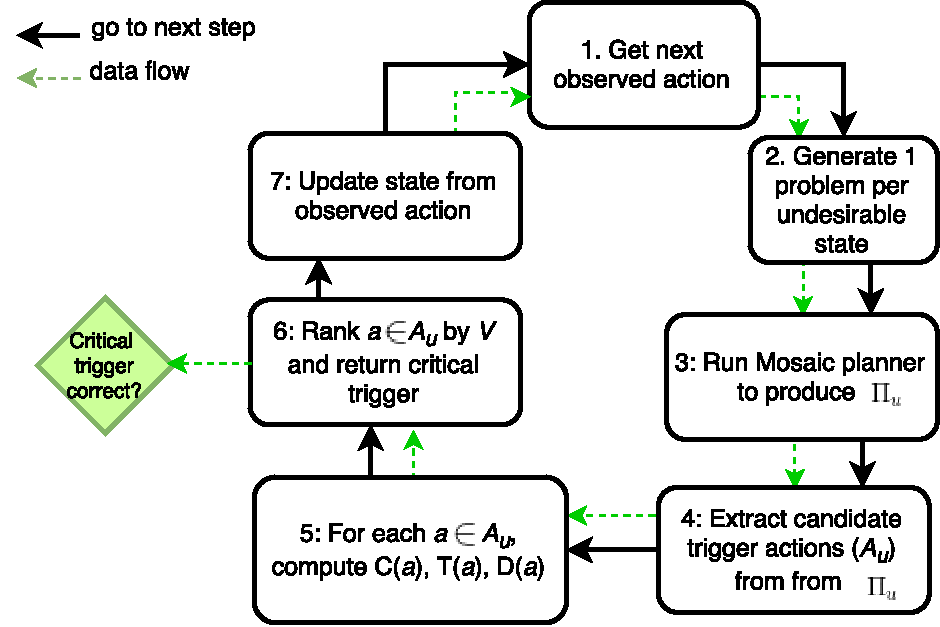
\includegraphics[width=0.5\textwidth]{img/algorithm.pdf}}
%\caption{Seven-step process for determining whether an observed action is a critical trigger action.}
%\label{fig:components}
%\end{figure}
%
%\section*{Evaluating the Undesirable State Recognition Function}
%We examine which factors impact the performance of detecting critical trigger actions using our metric function $V$. The \emph{independent variables} of the study are summarized in Table~\ref{tab:exp}, and include the weights for V, the problems, the percentage of extraneous actions, and the percentage of actions ``removed'' to emulated partial observability.
%
%Objective weights vary between a single metric, pairs of metrics and all three metrics with equal weights. We decided on these objective weight settings in order to identify which metrics (or their combinations) are sensitive to partial observability and extraneous actions separately. 
%
%
%We begin with results from a user study on cyber-security that motivated our work. This domain will be referred to as the \texttt{PAG} in our evaluation. For traces from the user study, we examine the impact of the objective weights (OW) used for in the objective function. Noisy sensing can lead to extraneous actions or missed observations, which complicates intervention. So we generalize these results to a set of benchmark domains from \cite{ramirez2009plan}, where greater experimental control allows us to evaluate the impact of extraneous actions (EA) and partial observability (PO). Thus, we expect some degradation in performance as the noise increases and observability decreases; the question is by how much? 
%
%\begin{table}[h]
%\begin{tabular}{|l|l|}
%\hline
%Variable                   & Settings                                           \\ \hline
%\begin{tabular}[c]{@{}l@{}}Objective Weights (OW)\\ (C,T,D)\end{tabular} &
%  \begin{tabular}[c]{@{}l@{}}(1,0,0), (0,1,0), (0,0,1), (0.33,0.33,0.33), (0.5,0.5,0), \\ (0.5,0,0.5), (0,0.5,0.5)\end{tabular} \\ \hline
%Planning Domains (PD       & PAG, blocks-words, navigator, ipc-grid+, logistics \\ \hline
%Partial observability (PO) & 25\%, 50\%, 75\%, 100\%                            \\ \hline
%Extraneous Actions (EA)    & 0\%, 50\%, 75\%, 100\%                             \\ \hline
%\end{tabular}
%\caption{Independent variables for evaluating impact of algorithm parameters and sensitivity to noisy data}
%\label{tab:exp}
%\end{table}
%
%
%The \emph{dependent variables} of the study include accuracy and computational overhead as measured in CPU time. For the cybersecurity domain, accuracy is defined as the percent true-positives only. For the benchmarks, we report accuracy in terms of percent true-positives and true-negatives. Computation time is included because ultimately we envision this being one component of a user supporting agent, which will require fast response. CPU time includes the time required to process each observation (one cycle of the process depicted in Figure~\ref{fig:components}) within a trial; this includes both generating the alternate plans and ranking the actions. 
%
%For each undesirable state, we use a plan generated by an automated planner as the `ground truth', which is referred to as UP. This is a fair assumption because the trace generation algorithm produces traces leading to the undesirable state (with varying levels of noise and observability). We measure accuracy with two evaluation metrics:
%\begin{itemize}
%\item Success rate in ignoring extraneous actions (Ignored EA)
%\item Success rate in flagging undesirable actions that appear in the ground truth plan (UP) (Flagged UP)
%\end{itemize}
%
%Ignored EA for an observation trace is computed as the count of instances where the observation was an extraneous action and it was not flagged as a critical trigger (count EA). It is given by the equation:
%\begin{equation}
%\textup{Ignored EA}\%= \frac{\textup{count EA}}{\textup{number of extraneous actions in trace}}\times 100
%\end{equation}
%Flagged UP for an observation trace is computed as the count of instances where the observation was an action from UP and the function V actually selected it as the critical trigger action. It is given by the equation:
%\begin{equation}
%\textup{Flagged UP}\%= \frac{\textup{count UP}}{\textup{number of UP actions in trace}}\times 100
%\end{equation}
%
%\subsection*{Cyber-security Domain (PAG)}
%We conducted an human subject experiment in a sand-boxed simulation environment to determine how non-expert users behave when presented with questionable computer security situations and to compare their actual observed behavior to their self-reports obtained via pre- and post-hoc surveys. Participants were presented with a desktop which includes common applications such as emailing, Web-browsing, social networking etc. Subjects were provided with written instructions on how to perform normal home computer user activities such as reading/sending email, installing software etc. While the normal computer activities were being performed, different events were simulated, without the subject's knowledge that can trigger threats and vulnerabilities of interest. These events included enticing user to disclose sensitive information (login names, passwords) to phishing sites over email and social media communications, responding to pop-ups asking the user to download a software, and reacting to malicious activities detected in the computer by an anti-virus program. Sixty-three human subjects participated in the study; their actions were collected into observation traces.
%
%
%We constructed a PDDL domain for the Personalized Attack Graph (\texttt{PAG}) to investigate what actions subjects might take amid the aforementioned threat scenarios.  We considered four undesirable states for this domain, resulting in four problem definitions. Figure~\ref{fig:trace} shows an actual observation trace indicating how the subject's observed actions (x axis) contributed to triggering the four undesirable states (the plans to do so are displayed as a sequence in each color). The y-axis shows how many steps in each undesirable plan (UP) have yet to be executed. When the dots remain horizontal, the actions are not in the undesirable plan; they are extraneous. For this trace, although the subject came close to triggering all four, only one actually happened (red color line - virus scan vulnerability). 
%
%\begin{figure}[t!]
% \centerline{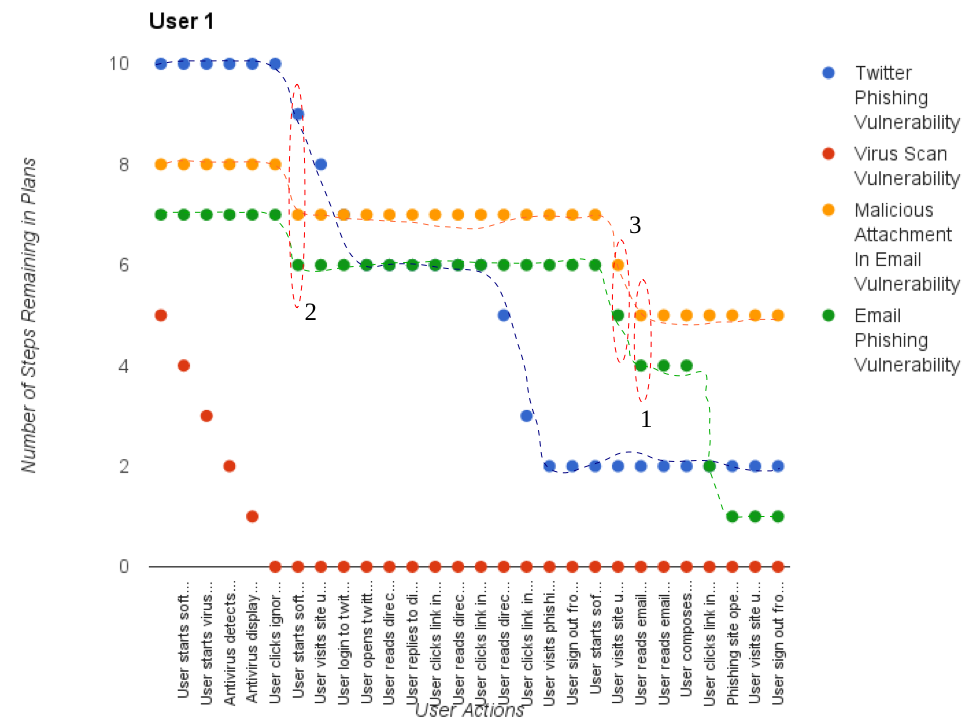
\includegraphics[width=\columnwidth, keepaspectratio=true]{img/user-study.png}}
% \caption{Observation trace from a human subject annotated with relation to undesirable plans (colored connected dots) and candidate trigger actions (in dotted ovals)}
% \label{fig:trace}
%\end{figure}
%
%We expected accuracy to be low because user logs offer unique challenges to the algorithm. Human users do not typically perform tasks in a ordered sequence. For example, some logs indicated that the subject was performing the same task repetitively, users had skipped a task to come back to it after an interval and more interestingly, some users were actively trying to trigger the vulnerabilities. These scenarios make it difficult to model a consistent state in a planning environment and affect candidate trigger actions being selected for the critical trigger ranking algorithm. To assess algorithm performance in a more controlled environment, we turned to benchmarks.
%
%
%\subsubsection*{PAG Results}
%Since activity logs captured during the experiment could not be properly controlled for extraneous and missing actions, we limit the assessment to accuracy and the effect of objective metric weightings on Flagged UP accuracy and CPU usage.
%
%The subjects were only provided with instructions to perform normal computer tasks. No restrictions were imposed on how they should interact with desktop environment (e.g., undo/redo tasks, exploring application features). Therefore, subject's goals while performing the tasks were unknown. Logs generated by two subjects were discarded because they did not complete the experiment. Considering 61 traces used in this evaluation, mean trace length was 39 (SD=21.13). The longest trace contained 120 observations, while the shortest was 10. 
%
%
%Mean accuracy was 59.53\% (SD=30.79) for all OW, but the weights exerted a significant influence on accuracy (\textit{F}=40866, \textit{p}$\ll$0). 
%The highest accuracy (mean=95.59\%,SD=2.13) occurred for two configurations of objective weight assignments: one that equally weighted all three metrics and one that equally weighted certainty and timeliness, ignoring desirability. 
%This suggests, by tagging specific undesirable actions and monitoring progress of plans, onset of critical states can be identified accurately in cyber-security scenario. Mean CPU time per cycle of the algorithm was 1.7 seconds (SD=0.45), suggesting that this algorithm could easily be integrated into an agent that mitigates cyber-security issues.
%
%
%\subsection*{Benchmark Domains}
%To generalize the results, we examine four domains from \cite{ramirez2009plan}. {\tt Block-Words} constructs one of 20 English words using 8 distinct letters. {\tt Grid-Navigation} forms paths through a connected graph to specific locations (goals). {\tt IPC-grid+} is a grid navigation with keys added at a restricted set of locations. {\tt Logistics} moves packages between locations. To keep the scale similar to the user study, we randomly selected four problems from each domain distribution.
%
%\subsubsection*{Trace Generation}
%To construct problem factors (EA, PO), we consider four problems from each benchmark domain. 
%For each problem, we generate noisy traces by incrementally building the plan starting from the initial state and interleaving it with actions from a set of pre-computed extraneous actions when the current state meets the preconditions of the extraneous action. Thus, the trace generation algorithm consists of two stages (1) computing the set of extraneous actions (EA) and (2) interleaving these extraneous actions.  Actions from the original undesirable plan are randomly removed from the interleaved trace to account for partial observability (PO).
%
%We use the Metric-FF \cite{hoffman2003ff} planner to generate extraneous actions because the planner's implementation offers configuration options to extract the relaxed planning graph and add/delete effects of actions. The challenge in generating extraneous actions to ensure it (1) does not introduce new facts that interfere with the progression of the 'ground truth' plan  or (2) does not delete the progress already made by the 'ground truth' plan. 
%
%We incrementally build the set of extraneous action starting from selecting actions that can be executed immediately after the goal state has been reached. By adding new actions, object types, and predicates to the domain model, the size of the resulting extraneous action set can be significantly increased to handle longer plans and create lengthy traces. The advantage of forward-expanding the set of extraneous actions starting at the goal state that at this stage the only condition we need to check is whether or not the chosen action deletes the goal state or not. Additionally, alternative actions available at the current level of the plan graph do not guarantee that they will not violate conditions (1) and (2) later. In certain occasions this could lead to traces where the same action is being done and undone repeatedly without making progress through the plan. We designed  trace generation algorithm that can overcome this challenge and builds the ground-truth plan incrementally from the initial state, while interleaving it with extraneous actions at relevant states.
%
%The Algorithm \ref{alg:extraneous} describes the process to compute the extraneous action pool for each problem in a domain.
%\begin{algorithm}
%    \caption{Extraneous Action Generation Algorithm}
%    \label{alg:extraneous}
%    \begin{algorithmic}[1]
%        \Procedure{extraneouspool}{$domain$,$problem,init$}
%        	\State $current\gets UP, EX_{goal}\gets \emptyset, state \gets init$
%        	\State $UP\gets Planner(domain,problem,state)$
%        	\ForAll{$a \in current$}
%        		\If{$Pre(a)\in state $} 
%        		\State $state\gets state\setminus Del(a)\cup Add(a)$
%        		\EndIf
%        	\EndFor
%        	\State $S_{goal}\gets state$
%        	\State select $action$ from Planning Graph such that:
%        	\State \hspace*{10pt}$action \notin UP$
%        	\State \hspace*{10pt}$Pre(action) \in S_{goal}$
%        	\State \hspace*{10pt}$state \setminus Del(action) \cup Add(action) \cap S_{goal} = \emptyset$
%        	\State $EX_{goal} \gets action$
%            \State \textbf{return} $EX_{goal}$
%        \EndProcedure
%    \end{algorithmic}
%\end{algorithm}
%We begin by computing the undesirable plan $UP$ using a planner. Then for the actions in $UP$ we modify the initial state by incorporating the effects of each action. The end of this loop translates the $state$ to the goal state for the problem. Then we generate the relaxed planning graph for the problem. We, then select actions from the planning graph such that actions that are not in $UP$ and the selected action is applicable in goal state and effects of the selected action does not remove the goal predicates. These actions form the extraneous action pool $EX_{goal}$. $EX_{goal}$ can be extended by modifying $S_{goal}$ with effects of a selected action from $EX_{goal}$, by following steps 4 through 5. The intuition is that once an extraneous action is executed at some state, the resulting state may enable additional extraneous actions. Repeat execution of this process generates a tree structure of extraneous actions with an action from $EX_{goal}$ as root. 
%
%
%We define percent extraneous actions (EA) in the observation trace (number of extraneous actions in trace / number of actions in plan) as a proxy for signal-to-noise ratio $[$0\%, 50\%, 75\%, 100\%$]$. Algorithm \ref{alg:noisytrace} describes our trace generation process. Starting from the initial state, actions in undesirable plan are added to the observation trace sequentially, including extraneous actions as appropriate. 
%This produces a final plan. Partial observability (PO) is computed by removing actions from the final plan are randomly selected and removed such that, PO\% (number of original actions in trace after removal / number of original actions in trace before removal) is one of $[$25\%, 50\%, 75\%, 100\%$]$. 
%
%\begin{algorithm}
%    \caption{Noisy Observation Trace Generation Algorithm}
%    \label{alg:noisytrace}
%    \begin{algorithmic}[1] % The number tells where the line numbering should start
%        \Procedure{noisytrace}{$domain$,$problem,init$}
%        	\State $current\gets UP, ea\gets 0, trace\gets \emptyset, state \gets init$
%        	\State $UP\gets Planner(domain,problem,state)$
%        	\ForAll{$a \in current$}
%        		\If{$Pre(a)\in state $} 
%        		\State $trace \gets trace \cup a$
%        		\State $state\gets state\setminus Del(a)\cup Add(a)$
%        		\EndIf
%        		\State $UP\gets Planner(domain,problem,state)$
%        		\State $current\gets UP$
%        		\If {$ea<required EA\%$}
%        		\State randomly select $action$ from $EX_{goal}$ if Pre($action$) $\in state$
%        		\State $trace \gets trace \cup action$
%        		\State update $ea, state, current$
%        		\EndIf
%        	\EndFor
%        	\State Fix PO\% in $trace$ by removing actions
%            \State \textbf{return} $trace$
%        \EndProcedure
%    \end{algorithmic}
%\end{algorithm}
%
%
%
%
%
%   \begin{table}[t]
%     \centering
%   \begin{small}
%   \resizebox{\columnwidth}{!}{
%	\begin{tabular}{|c|ccc|ccccccc|}
%		\hline
%	    & \multicolumn{10}{c|}{Mean Ignored EA\%} \\ \cline{2-11}
%		\multirow{3}{*}{Domain}  & \multicolumn{3}{c|}{EA\% in trace} & \multicolumn{7}{c|}{OW Assignments  (C,T,D)} \\ \cline{2-11} 
%		& 50\% & 75\% & 100\%
%%		& (0,0,1) & (0,.5,.5) & (0,1,0) & (.3,.3,.3) & (.5,0,.5) & (.5,.5,0) & (1,0,0) \\ \hline
%		& (0,0,1) & (0,0.5,0.5) & (0,1,0) & (0.3,0.3,0.3) & (0.5,0,0.5) & (0.5,0.5,0) & (1,0,0) \\ \hline
%		\texttt{blo} & \begin{tabular}[c]{@{}c@{}}95.2 \\ (8.0)\end{tabular} & \begin{tabular}[c]{@{}c@{}}97.6\\ (3.6)\end{tabular} & \begin{tabular}[c]{@{}c@{}}97.3\\ (3.2)\end{tabular} & \begin{tabular}[c]{@{}c@{}}99.0\\ (1.6)\end{tabular} & \begin{tabular}[c]{@{}c@{}}94.7\\ (6.7)\end{tabular} & \begin{tabular}[c]{@{}c@{}}95.2\\ (6.2)\end{tabular} & \begin{tabular}[c]{@{}c@{}}95.4\\ (7.0)\end{tabular} & \begin{tabular}[c]{@{}c@{}}98.6\\ (1.7)\end{tabular} & \begin{tabular}[c]{@{}c@{}}95.4\\ (7.0)\end{tabular} & \begin{tabular}[c]{@{}c@{}}98.6\\ (1.7)\end{tabular} \\ \hline
%		\texttt{ipc} & \begin{tabular}[c]{@{}c@{}}86.4\\ (14.4)\end{tabular} & \begin{tabular}[c]{@{}c@{}}89.9\\ (11.6)\end{tabular} & \begin{tabular}[c]{@{}c@{}}89.9\\ (10.7)\end{tabular} & \begin{tabular}[c]{@{}c@{}}95.6\\ (3.7)\end{tabular} & \begin{tabular}[c]{@{}c@{}}83.2\\ (13.0)\end{tabular} & \begin{tabular}[c]{@{}c@{}}81.3\\ (12.9)\end{tabular} & \begin{tabular}[c]{@{}c@{}}83.9\\ (15.1)\end{tabular} & \begin{tabular}[c]{@{}c@{}}95.9\\ (3.4)\end{tabular} & \begin{tabular}[c]{@{}c@{}}85.1\\ (14.8)\end{tabular} & \begin{tabular}[c]{@{}c@{}}95.9\\ (3.4)\end{tabular} \\ \hline
%		\texttt{log} & \begin{tabular}[c]{@{}c@{}}97.9 \\ (4.4)\end{tabular} & \begin{tabular}[c]{@{}c@{}}96.7\\ (5.7)\end{tabular} & \begin{tabular}[c]{@{}c@{}}96.1\\ (5.4)\end{tabular} & \begin{tabular}[c]{@{}c@{}}98.4\\ (2.8)\end{tabular} & \begin{tabular}[c]{@{}c@{}}94.4\\ (7.2)\end{tabular} & \begin{tabular}[c]{@{}c@{}}96.1\\ (3.6)\end{tabular} & \begin{tabular}[c]{@{}c@{}}96.2\\ (6.9)\end{tabular} & \begin{tabular}[c]{@{}c@{}}98.6\\ (2.6)\end{tabular} & \begin{tabular}[c]{@{}c@{}}96.2\\ (6.9)\end{tabular} & \begin{tabular}[c]{@{}c@{}}98.5\\ (2.6)\end{tabular} \\ \hline
%		\texttt{nav} & 100 (0) & 100 (0) & 100 (0) & 100 (0) & 100 (0) & 100 (0) & 100 (0) & 100 (0) & 100 (0) & 100 (0) \\ \hline
%	\end{tabular}
%	}%	
%   \end{small}
%	\caption{Mean Ignored EA\%  (and standard deviation) for benchmark domains for levels of EA\% in observation trace and objective weight assignment classes. The left three columns combine mean Ignored EA\% for OW assignments across all values of $\alpha$ and breaks mean Ignored EA\% down by EA\% in trace. The right OW columns breaks down mean Ignored EA\% by specific $\alpha$ value for all levels of EA\% in observation trace.}
%	\label{tab:ignoredeaforlevels}
%\end{table}
%
%
%\begin{table}[t]
%	\centering
%\begin{small}
%\resizebox{\columnwidth}{!}{
%	\begin{tabular}{|c|c c c c|c c c c c c c|}
%		\hline
%		& \multicolumn{11}{c|}{Mean Flagged UP\%} \\ \cline{2-12} 
%		\multirow{3}{*}{Domain} & \multicolumn{4}{c|}{PO\% in trace} & \multicolumn{7}{c|}{OW Assignments (C,T,D)} \\ \cline{2-12} 
%%		& 25\% & 50\% & 75\% & 100\% & (0,0,1) & (0,.5,.5) & (0,1,0) & (.3,.3,.3) & (.5,0,.5) & (.5,.5,0) & (1,0,0) \\ \cline{1-12} 
%		& 25\% & 50\% & 75\% & 100\% & (0,0,1) & (0,0.5,0.5) & (0,1,0) & (0.3,0.3,0.3) & (0.5,0,0.5) & (0.5,0.5,0) & (1,0,0) \\ \cline{1-12} 
%		
%		\texttt{blo} & \begin{tabular}[c]{@{}c@{}}20.1\\ (21.2)\end{tabular} & \begin{tabular}[c]{@{}c@{}}23.6\\ (14.4)\end{tabular} & \begin{tabular}[c]{@{}c@{}}31.8\\ (19.3)\end{tabular} & \begin{tabular}[c]{@{}c@{}}40.2\\ (26.1)\end{tabular} & \begin{tabular}[c]{@{}c@{}}9.2\\ (7.6)\end{tabular} & \begin{tabular}[c]{@{}c@{}}24.8\\ (20.1)\end{tabular} & \begin{tabular}[c]{@{}c@{}}37.0\\ (17.5)\end{tabular} & \begin{tabular}[c]{@{}c@{}}46.5\\ (24.9)\end{tabular} & \begin{tabular}[c]{@{}c@{}}19.0\\ (7.6)\end{tabular} & \begin{tabular}[c]{@{}c@{}}46.8\\ (24.9)\end{tabular} & \begin{tabular}[c]{@{}c@{}}19.0\\ (7.6)\end{tabular} \\ \hline
%		\texttt{ipc} & \begin{tabular}[c]{@{}c@{}}6.9\\ (18.8)\end{tabular} & \begin{tabular}[c]{@{}c@{}}25.6\\ (20.0)\end{tabular} & \begin{tabular}[c]{@{}c@{}}42.3\\ (32.0)\end{tabular} & \begin{tabular}[c]{@{}c@{}}50.8\\ (36.2)\end{tabular} & \begin{tabular}[c]{@{}c@{}}9.7\\ (5.2)\end{tabular} & \begin{tabular}[c]{@{}c@{}}46.5\\ (34.7)\end{tabular} & \begin{tabular}[c]{@{}c@{}}47.9\\ (35.0)\end{tabular} & \begin{tabular}[c]{@{}c@{}}47.5\\ (35.8)\end{tabular} & \begin{tabular}[c]{@{}c@{}}10.5\\ (4.9)\end{tabular} & \begin{tabular}[c]{@{}c@{}}47.1\\ (35.9)\end{tabular} & \begin{tabular}[c]{@{}c@{}}10.6\\ (4.9)\end{tabular} \\ \hline
%		\texttt{log} & \begin{tabular}[c]{@{}c@{}}18.4\\ (27.4)\end{tabular} & \begin{tabular}[c]{@{}c@{}}16.4\\ (20.1)\end{tabular} & \begin{tabular}[c]{@{}c@{}}20.4\\ (19.5)\end{tabular} & \begin{tabular}[c]{@{}c@{}}31.5\\ (17.8)\end{tabular} & \begin{tabular}[c]{@{}c@{}}15.2\\ (10.6)\end{tabular} & \begin{tabular}[c]{@{}c@{}}20.9\\ (28.2)\end{tabular} & \begin{tabular}[c]{@{}c@{}}24.6\\ (25.4)\end{tabular} & \begin{tabular}[c]{@{}c@{}}27.2\\ (28.5)\end{tabular} & \begin{tabular}[c]{@{}c@{}}18.3\\ (10.1)\end{tabular} & \begin{tabular}[c]{@{}c@{}}27.2\\ (28.5)\end{tabular} & \begin{tabular}[c]{@{}c@{}}18.3\\ (10.9)\end{tabular} \\ \hline
%		\texttt{nav} & \begin{tabular}[c]{@{}c@{}}14.8\\ (19.1)\end{tabular} & \begin{tabular}[c]{@{}c@{}}32.4\\ (22.6)\end{tabular} & \begin{tabular}[c]{@{}c@{}}45.2\\ (27.4)\end{tabular} & \begin{tabular}[c]{@{}c@{}}61.7\\ (39.8)\end{tabular} & \begin{tabular}[c]{@{}c@{}}14.1\\ (3.4)\end{tabular} & \begin{tabular}[c]{@{}c@{}}56.8\\ (33.7)\end{tabular} & \begin{tabular}[c]{@{}c@{}}56.8\\ (33.7)\end{tabular} & \begin{tabular}[c]{@{}c@{}}56.8\\ (33.7)\end{tabular} & \begin{tabular}[c]{@{}c@{}}14.1\\ (3.43)\end{tabular} & \begin{tabular}[c]{@{}c@{}}56.8\\ (33.7)\end{tabular} & \begin{tabular}[c]{@{}c@{}}14.1\\ (3.4)\end{tabular} \\ \hline
%	\end{tabular}
%	}%
%\end{small}
%	\caption{Mean Flagged UP\%  (and standard deviation) for benchmark domains for levels of PO\% in observation trace and objective weight assignment classes. The left four columns combine mean Flagged UP\% for OW assignments across all values of $\alpha$ and breaks mean Flagged UP\% down by PO\% in trace. The right OW columns breaks down mean Flagged UP\% by specific $\alpha$ value for all levels of PO\% in observation trace.}
%	\label{tab:flaggedupforlevels}
%\end{table}
%
%
%
%\subsubsection*{Benchmark Results}
%We review the overall accuracy of our algorithm in benchmark domains by evaluating how well it ignores extraneous actions and flags undesirable actions in the ground truth plan.
%
%\textbf{Ignoring Extraneous Actions}\\
%When encountered with extraneous actions in the trace, the algorithm must be able to avoid flagging it as critical. We define mean Ignored EA\% percentage for a domain as: (sum of Ignored EA\% per trial / number of trials with EA\%$>$0). Table \ref{tab:ignoredeaforlevels} shows how mean Ignored EA\% varies with the noise level of the observation trace and objective weight assignments.
%
%Results show that our algorithm consistently ignores extraneous actions for all benchmark domains. This high accuracy rate can be attributed to our process of selecting critical trigger actions. Since candidate trigger actions are extracted from a set of alternative plans leading to the same undesirable state, the likelihood of true extraneous actions to appear in the set of alternative plans is low. This reduces the likelihood of false-positives in the trace.
%
%
%The OW combinations significantly influence Ignored EA\%  ($p<0.05$ for the \texttt{blo}, \texttt{ipc} and \texttt{log} domains). Post-hoc analysis using TukeyHSD at $\alpha=0.05$ shows that across domains, OW combinations that do not consider the timeliness metric better perform at ignoring extraneous actions than combinations that include timeliness. This is because timeliness metric is not sensitive to extraneous actions in the trace. As a result, the objective function can not sufficiently differentiate between extraneous actions and actions in ground truth plan, leading to false positives.Because timeliness metric captures progress yet to be made from current state to triggering the undesirable state in terms of remaining steps, in the presence of extraneous actions, which do not contribute to progress toward the undesirable state, the metric does not sufficiently demote the extraneous action in the candidate action set, leading to false-positives. 
%In contrast, certainty and desirability metrics look for occurrences of an action in undesirable plans. As extraneous actions do not occur in undesirable plans, both metrics are capable of filtering extraneous actions from the candidate action pool by minimizing objective function value and preventing them from being selected as the critical trigger.
%
%
%\textbf{Flagging Undesirable Actions}\\
%Flagged UP\% captures how well the algorithm flags observations as critical triggers given that the observation appears in an undesirable plan treated as ground truth. We first look at Flagged UP\% in traces with 0\% noise and full observability (i.e., best-case scenario) to establish an upper bound to the metric.
%
%Table \ref{tab:flagupupperbound} shows a very large range (Max-Min) for Flagged UP\%. This indicates that although the only variable for this sample is OW, Flagged UP\% is also sensitive to other external factors that have not been accounted for in our proposed objective function. The challenge lies in identifying these external factors and determining their relationship so that the objective function can be tuned to improve accuracy. This will be the main focus of our future work. 
%
%Table \ref{tab:flaggedupforlevels} shows that Flagged UP\% also increases when observability increases in the trace. Factor analysis using one-way ANOVA for OW shows that this positive effect is significant ($p<0.05, df=6$) for all four benchmark domains. Interestingly, high Flagged UP\% was reported for OW combinations that consider timeliness: specifically for configurations, certainty-timeliness-desirability with equal weighting, certainty-timeliness with equal weighting and desirability-timeliness with equal weighting. Post-hoc analysis using TukeyHSD at $\alpha=0.05$ shows that this difference is significant. Thus, we conclude that the timeliness metric can improve the true-positive rate, yielding higher precision for the algorithm. The timeliness metric is sensitive to partial observability because it sufficiently captures distance to triggering an undesirable state, which is a consistent indicator of the progress is being made. Even with partial observability, the remaining steps of a plan change in such a way that it can be tracked and correctly reflected in the objective function. Accuracy of the certainty and desirability metrics lowers as partial observability increases because they consider occurrences of an action. 
%
%
%\textbf{Computational Overhead}\\
%For each benchmark domain, we calculated the average CPU time per cycle for problem factors (EA and PO). As shown in Table \ref{tab:cpu2}, we found differences due to observation trace factors; two-way ANOVA on EA and PO showed significant main effects and interaction effects ($p<$0.05) for \texttt{ipc}, \texttt{log} and \texttt{nav} domains.
%
%
%\begin{table}[t]
%  \centering
%    \resizebox{0.7\columnwidth}{!}{
%  \begin{tabular}{|l|r|r|r|r|r|r|r|r|r|}
%    \hline
%    \multirow{2}{*}{Domain}
%  &  \multicolumn{4}{c|}{EA\% in trace} & \multicolumn{4}{c|}{PO\% in trace} & \\ \cline{2-9}
% & 0\% & 50\% & 75\% & 100\% & 25\% & 50\% & 75\% & 100\% & $\Delta$ \\
%    \hline
%{\tt blo} & 2.3  & 2.2  & 2.2  & 2.2  & 2.2  & 2.2  & 2.3  & 2.2  & 1.4  \\
%{\tt ipc} & 4.9  & 4.8  & 4.9  & 4.9  & 4.9  & 4.9  & 4.9  & 4.8  & 0.9  \\
%{\tt log} & 1.7  & 1.7  & 1.6  & 1.7  & 1.7  & 1.7  & 1.7  & 1.7  & 0.5  \\
%{\tt nav} & 1.3  & 1.3  & 1.3  & 1.3  & 1.3  & 1.3  & 1.3  & 1.3  & 0.5  \\
%    \hline
%  \end{tabular}
%  	}%resize box
%  \caption{Mean CPU time in seconds for problem factors for each domain. $\Delta$ is the difference between the max and min times for each domain.}
%  \label{tab:cpu2}
%\end{table}
%
%\begin{table}[!t]
%	\centering
%    \begin{small}
%	\begin{tabular}{|l|c|c|c|c|}
%		\hline
%		\multirow{2}{*}{Domain} & \multicolumn{4}{c|}{Flagged UP\%} \\ \cline{2-5} 
%		& Mean   & SD     & Min    & Max    \\ \hline
%		\texttt{blo}                     & 37.12  & 24.83  & 6.12   & 77.78  \\ 
%		\texttt{ipc}                     & 43.27  & 30.55  & 0.00   & 90.00  \\ 
%		\texttt{log}                     & 31.77  & 17.27  & 12.82  & 66.67  \\ 
%		\texttt{nav}                     & 61.68  & 40.31  & 14.10  & 100.00 \\ \hline
%	\end{tabular}
%\end{small}
%		\caption{Flagged UP\% for traces with 0\% EA and 100\% PO for \texttt{Block-words} (\texttt{bw}), \texttt{IPC-grid+} (\texttt{ipc}), \texttt{Logistics} (\texttt{log}), and \texttt{Grid-Navigation}   (\texttt{nav}) domains}
%		\label{tab:flagupupperbound}
%\end{table}
%
%\section*{Summary and Future Work}
%We have described a variant of plan recognition that can help identify intervention points to help a user avoid undesirable states while interacting with a computer. Our approach views the decision of when to intervene as a multi-objective optimization problem that optimizes three domain-independent objective metrics: certainty, timeliness and desirability. We tested our algorithm on both benchmark domains and human subject data from a cyber-security experiment. Results show that, across all benchmark domains, certainty and desirability metrics perform well in ignoring extraneous actions, while the timeliness metric and it's combinations with certainty and desirability perform well in identifying true positives. We identified two metrics that are sensitive to noise in action based observation traces and a metric that is sensitive to partial observability of actions.
%
%However, the low percentage of true-positives in the best case scenario indicate that the metrics are not good enough in their raw form in dealing with partial observability. Therefore, metrics must be developed to evaluate the contribution of less frequent actions appearing in alternative plans. Evaluation of the effects of objective weight metrics, shows that desirability metric does not adequately downgrade the effect of certainty and timeliness. This indicates that objective weight assignments require an in depth look into multi-objective optimization techniques to find the optimal combination of weights over metrics.
%Furthermore, concepts behind certainty metric touches upon landmarks in planning. We will further explore these aspects in the future.





%%%%%%%%%%%%%%%%%%%%%%%%%%%%%%%%%%%%%%%%%%%%%%%%%%%%%%%%%%%%%%%%%
\chapter{Design of a Soft Intervention Model to Support Human Users During Cognitively Engaging Tasks}
\label{chap:soft}
%%%%%%%%%%%%%%%%%%%%%%%%%%%%%%%%%%%%%%%%%%%%%%%%%%%%%%%%%%%%%%%%%
\section*{Introduction}
\label{sec:introduction}
When a human user is learning to use a new software application, it can be helpful to have a passive observer software agent that can intervene to help the user reach his intended goal. This is particularly important when using the software imposes a significant cognitive load on the user and as a result the user's plan to accomplish the intended goal can become vulnerable to unintended actions or events. A previous study \cite{byrne2016} showed that users pay more attention to the benefits of activities than the risk; they have goals that they want/need to achieve and are willing to take the risk to achieve them. Because the human user is more inclined to prioritize achieving the goal above the risks, given a cognitively engaging task, users may take actions that will lead to undesirable consequences. In the least harmful case, the undesirable consequence could be the user quitting without completing the task. In the worst case, the user may be misled and become an unwitting accomplice to some security/privacy breach (e.g., a customer using an online banking software becoming vulnerable to a cross-site scripting attack). We propose intervention as an approach to help human users avoid undesirable states while engaged in a cognitively taxing task. We ask two important questions:
\begin{itemize}
\item When should the user be intervened?
\item How to support the task completion through intervention?
\end{itemize}

The basic, fully deterministic version of the planning problem is: given a set of applicable actions, a starting state and a goal state, find a sequence of actions (a \textit{plan}), which modifies the starting state to the goal state, while optimizing some utility function (e.g., plan cost). Automated planners translate the planning problem to a search problem using an internal representation such as propositional, STRIPS or state-variables. Then a search strategy is applied starting from the initial state and repeatedly expanding successor states until the goal state is produced. Depending on the search strategy, the solution to the planning problem may be optimal or sub-optimal.

However, when human planners are in the picture, they may not want to cede control to the automated planner entirely. More relevant in domains like cyber-security, the human users may also have implicit, yet complementary goals. For example, consider the online banking application. The user would like transfer money to an account with the fewest number of steps. At the same time, the user would also like to complete this task without having his password stolen. In certain cases, the human user may not know the full set of effects of their actions (e.g, not knowing that a cross-site scripting vulnerability can be exploited in the banking system) or may not be thinking about the effects at all. When modeling more complex domains, it may be difficult to give the automated planner an accurate representation of the application itself, leading to unsafe plans being suggested. Similarly, human planners working in complex domains may make mistakes and commit to plans that are not safe. These issues affect both expert and non-expert human users when solving planning problems albeit in varying degrees of difficulty.

The problem of undesirable consequences prediction is assessing whether an action is likely to lead to undesirable consequences. When should the user be intervened? The most straightforward class of undesirable actions is when the effect of the action is the undesirable consequence. The intervention model that deals with the first class of undesirable actions is called \textbf{hard intervention}, and is used to block the user from making further progress. Identifying actions, which provide conditions that can be exploited to activate the undesirable state is called \textbf{soft intervention}. Soft intervention is used as a supportive model in which the user advances towards the goal while avoiding undesirable consequences. Our investigation of hard and soft intervention concentrates on how human users solve the Rush Hour Puzzle. In the standard version of the puzzle, the player moves vehicles on a board to unblock a target vehicle so that the target vehicle can be moved to the exit. We modify the standard version of the Rush Hour puzzle by introducing a forbidden vehicle. If the user moves the forbidden vehicle at some time during the game, the user triggers the undesirable state. The solution to the puzzle is a sequence of moves that changes the starting position of the target vehicle to be at the exit position. The player has complete knowledge about the goal (target vehicle must be at the exit position) and the actions that can be executed to reach the goal. We identify actions that move the forbidden vehicle as \textit{dangerous} moves. The dangerous moves allow us to categorize players' solutions into safe (the solution does not contain any dangerous moves) and unsafe (solution contains at least one dangerous move). The Rush Hour puzzle is designed such that there is at least one solution that contains only legal moves. Effects of any dangerous move cause the undesirable consequence. The player does not know what the specific dangerous moves are, but he knows that \textit{some} moves are dangerous. Therefore, any partial solution that has been safe until now can turn into an unsafe solution.  In this study, we use two methods to address the question of how to support task completion. Hard intervention occurs at the same time point when the player makes a dangerous move. The hard intervention process forces the user to choose a different, safe move by blocking the dangerous move. Soft intervention is used upon recognizing that the player's solution will likely lead to triggering the undesirable consequence in the future. This mode of intervention gives some time for the player to modify his solution to avoid the undesirable state. The intervention step issues an alert with hints the user can choose that will help avoid the undesirable consequence. 

Because the puzzle can be solved without making any dangerous move, and the user has been notified to avoid dangerous moves, we use the event of making a dangerous move as an indicator of the user ignoring the undesirable consequence of the puzzle solving task. Hard intervention is suitable in this situation because at that point, the user has moved so far away from a safe solution that the undesirable consequence is imminent and blocking the action to prevent the undesirable consequence takes priority. On the other hand, soft intervention allows us to evaluate the different types of help the user will find most effective at different stages of the solution. This is because when soft intervention occurs, the undesirable state is not imminent but still developing. When the user makes certain moves the partial solution gets closer to the undesirable state. We use an automated planner to find an optimal solution to the puzzle that contains only safe moves. This optimal solution provides a reference to compare and evaluate the user's partial solution.


To design effective automated assistant tools tailored to the human user, we need knowledge of how the user responds when he is actually placed in a situation that demands significant cognitive effort. Observing users performing actions is preferred over relying on self reporting because studies have been able to verify user's reports on their usage of computers have uncovered lower actual values than reported rates of some behaviors \cite{govani2005, howe2012psychology}. Based on these findings we designed a web based simulator framework to allow human users engage in a Rush Hour puzzle solving task. In addition to imposing a cognitive load on the user, the puzzle solving activity also prompts goal directed behavior in human users in a naturalistic setting. Furthermore, humans can increase their understanding of the game and their skills over time. This setup provides a natural analogy to what happens when a human is using a new website or a new software, where mistakes are typically more common for first time users and unskilled users.

The simulation framework operates in two modes. In the first mode of operation, the user solves the puzzle without any intervention. As the subject performs the puzzle solving task, the system records the events that occur on the interface. These event logs are used to extract unique user behavior patterns that are indicators of the user's puzzle solving aptitude. For example, what movements indicate that the user is getting further away from the solution? Is the user still in the learning phase and therefore mostly doing exploratory moves? We use these patterns to define features of users' solutions for the puzzle. Using the feature set, we generate learned models to predict whether or not the user's solution will reach an undesirable state before it actually happens. The second mode of operation integrates a learned intervention model into the simulation framework. This allows us to evaluate the effectiveness of our soft intervention model that learns to intervene by recognizing human user behavior patterns. In order to help guide the user toward the solution, we designed a set of hints - pieces of information about the Rush Hour search problem. Our underlying hypothesis is that intervention will be more effective when the user acts as a partner with the system he is interacting with. An automated planner is integrated into the framework to generate answers for the hints. The automated planner produces a optimal solution for a specific Rush Hour puzzle, which provides a reference solution that we can compare to the user's solution.

As the user continues to solve a puzzle, the framework records the partial solution the user generates. This partial solution is then used to compute the feature values and given to the learned model to make a prediction on whether or not the user needs intervention in the current state. If intervened, the user is shown a set of hints. Based on the user's choice of a hint the answer is provided. The hints do not directly give the complete solution (i.e., steps to solve the puzzle from the current state). Instead, the hints are a form of a constrained probe, which allows the user to explore the search space of the puzzle while avoiding the undesirable state.

Studies have shown that users want some positive outcome from their action and are willing to accept that negative outcomes are a possibility\cite{good2005stopping,debatin2009facebook,byrne2016}. To this end, a solution that simply blocks them from taking the action is not sufficient. Instead, it also needs to assist the user in deciding what to do next. The first contribution of our work is the soft intervention model, which addresses this issue following a user centered design methodology. The user centered design approach ensures that the needs of end-users are fulfilled by involving users throughout the design and development process. The second contribution of this work is the simulation framework, which facilitates collection of human user behavior data to design the intervention model and also evaluate how the human user responds to soft intervention actions in situ.
%
%soft intervention the helping agent says: i don't think you are going to click the bad car now but I think you need help.
%hard intervention the helping agent says: whoa u moved the forbidden car, you have gone as far as you possibly can away from the solution. i don't think you know how to get to the optimal solution that is safe.
%so my question is how much trouble are they in. how much help do they need?
%hard intervention is when you are in a lot of trouble. nowhere else to go
%soft intervention is when you are slowly digging the hole
%
%how are these two questions important?
%what are the shortcomings of the current solutions in planning? (this i don't know for sure. check case based planning, maybe more relevant than plan recognition)
%
%
\section*{The Rush Hour Puzzle}
\label{sec:rushhourpuzzle}
%about the game
The Rush Hour puzzle is a children's game (for ages 8 and above), that is played on a $n \times n$ square grid. Several cars (size=2) and trucks (size=3) are arranged on the board, which has only one exit. Figure \ref{fig:start} shows a sample initial puzzle configuration on a $6 \times 6$ grid. Vehicles T0, $\ldots$, T2 are trucks and C0, $\ldots$, C7 are cars, with C0 being the special target car. The vehicles can only move in the same orientation in which they were initially placed, i.e., vertical vehicles can only move up and down while horizontal vehicles can move left and right. Vehicles can be moved one at a time and into adjacent empty spaces. The objective of the game is to move the vehicles on the board in such a way that the target car (shown in red in Figure \ref{fig:start}) can be moved out of the exit on the right edge of the board. Solution to the Rush Hour puzzle is a sequence of legal moves that transforms the initial board state shown in \ref{fig:start} to the goal state in \ref{fig:end}. For the puzzle shown in Figure\ref{fig:whole}, the shortest solution, if the number of moves is considered as the optimizing criteria, consists of 21 moves. If optimized for the number of vehicles moved, the puzzle can be solved optimally by moving only 8 vehicles. 
\begin{figure}[!pbt]
  \centering
  \subfloat[Initial game state]{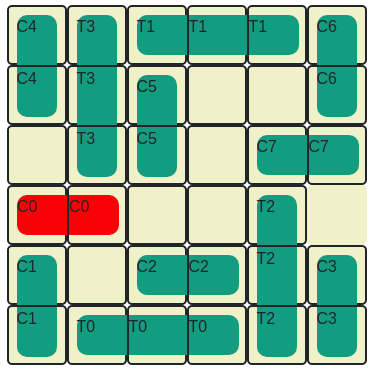
\includegraphics[width=0.4\textwidth]{img/start.png}\label{fig:start}}
  \hfill
  \subfloat[End game state]{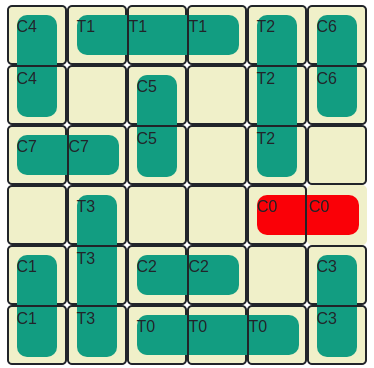
\includegraphics[width=0.4\textwidth]{img/end.png}\label{fig:end}}
  \caption{Rush Hour Board Configurations}
  \label{fig:whole}
\end{figure}
Flake et al. \shortcite{flake2002} showed that the generalized form of the Rush Hour puzzle (GRH) is PSPACE complete. GRH adopts two modifications to the standard problem. First, the grid size is allowed to be a rectangle of arbitrary width and height. Second, the exit is located at any position on the perimeter of the grid. In our experiments we are using the standard version of the puzzle (i.e., $6\times6$ grid with the fixed exit point). We modified the standard version of the Rush Hour puzzle to simulate the presence of an undesirable consequence by introducing a \textit{forbidden} vehicle.  Any action that moves the forbidden vehicle is set to cause the undesirable consequence. The forbidden vehicle introduces a constraint to the set of possible moves the user can make.

Our experiments found that, even in the standard version of the puzzle, human users find it quite difficult to free the target vehicle in certain configurations containing intricate dependencies between vehicles. The vehicle movement constraint introduced by the presence of the forbidden vehicle adds an extra level of difficulty to the user's puzzle solving task. Also, because our study analyses how human users approach solving a cognitively engaging problem, in order for us to easily collect data, it is critical that the users were willing to participate in the task. The Rush Hour puzzle addresses this requirement well. Although, the puzzle is a game, the environment is rich enough to simulate undesirable consequences and also offer the users a task that is challenging enough. We adopt the formal definition of a Rush Hour instance from \cite{flake2002}. 

\begin{definition} 
A Rush Hour instance is a tuple $\langle w,h,x,y,n,\mathcal{V}\rangle$ such that:
\begin{itemize}
\item $(w,h) \in {\mathbb{N}}^2$ are the grid dimensions. In the standard version, $w=h=6$
\item $(x,y) \in {\mathbb{N}}^2$ are the coordinates of the exit, which must be on the perimeter of the grid.
\item $n \in \mathbb{N}$ the number of non-target vehicles
\item $\mathcal{V}=\lbrace v_0, \ldots, v_n \rbrace$ is the set of $n+1$ vehicles comprised of cars $(\mathcal{C})$ and trucks $(\mathcal{T})$. Note that $|\mathcal{V}|=|\mathcal{C}|+|\mathcal{T}|$
\\$v_i \in \mathcal{C}$ is identified as $\lbrace C_0,\ldots,C_l \rbrace$, where $l=|\mathcal{C}|-1$ and $v_i \in \mathcal{T}$ is identified as $\lbrace T_0,\ldots,T_m \rbrace$, where $m=|\mathcal{T}|-1$.
\\A vehicle is a tuple $v_i=\langle x_i,y_i,o_i,s_i \rangle$, where $(x_i,y_i) \in {\mathbb{N}}^2$ are the vehicle coordinates, $o_i \in \lbrace N,E,S,W\rbrace$ is the vehicle orientation for North, East, South, West, $s_i \in \lbrace2,3\rbrace$ is the vehicle size and $C_0$ is the target vehicle.
\end{itemize}
\label{rushdef}
\end{definition}

Following the \dref{rushdef}, Flake et al. also defines the \textit{solution} to a Rush Hour instance:
\begin{definition} 
The solution to a Rush Hour instance is a sequence of $m$ moves, where each move consists of a vehicle identifier $i$, a direction that is consistent with the initial orientation of $v_i$, and a distance. Each move, in sequence must be consistent with itself and with the configuration prior to the move. Further, in order to move a distance $d$ the configuration must be consistent for all $d^\prime$ such that, $0\leqslant d^\prime \leqslant d$ (i.e., a vehicle can not jump over other vehicles on its path).
\end{definition}

\subsection*{The Rush Hour Puzzle as a Planning Problem}
\label{sec:rushhourasaplanningproblem}
Automated planning allows us to define the Rush Hour puzzle as a planning problem. The planning problem is given a set of operators, an initial state description and a goal state description finding a sequence of operator instances such that performing them in order from initial state will modify the initial state into the goal state. The world is typically viewed to consist of atomic facts (state variables). The actions make some facts true and some facts false. A planning problem can be formalized in many ways such as a state transition system (a graph where nodes represent the states and arcs represent the actions) or using situation calculus (first order logic to reason about actors in time). In this work we model the problem as a state transition system. However, we use a succinct representation of the transition system instead of the graph model, called STRIPS \cite{fikes1971strips}.

In STRIPS language, state variables have the domain $\lbrace True, False \rbrace$ and an operator consists of two sets of state variables \textbf{preconditions} and \textbf{effects}. Preconditions are state variables that needs to be \textit{True} for the operator to execute. Effects are state variables that will be \textit{True} (and \textit{False}) as a result of the operator executing . We now present a formal definition of a STRIPS domain and planning problem. In STRIPS, a planning task is defined using a planning domain and a planning problem.

\begin{definition}
A STRIPS planning domain is a tuple $\mathcal{D}=\langle F, Op\rangle$, where $F$ is a finite set of  state variables (predicates) and $Op$ is the set of operator schema. An operator schema $op \in Op$ is a tuple $ op = \langle Pre(op), Add(op), Del(op)\rangle$ that consists of preconditions, add and delete effects respectively, where $Pre(op)$, $Add(op)$, $Del(op)$ are all subsets of $F$. Predicates and operator schema have parameter lists and can be instantiated with objects (defined later). An instantiated operator (action) $op$ is applicable in a state $s$ if predicates in $Pre(op)$ are \textit{True} in $s$. A state transition induced by an action $op$ in a state $s$ is defined as a function $\delta$:
\begin{equation*}
\delta (s,op) = \left\{\begin{matrix}
s\setminus Del(op) \cup Add(op) & Pre(op) \subseteq s\\ 
undefined & otherwise
\end{matrix}\right.
\end{equation*}
\end{definition}

\begin{definition}
A STRIPS planning problem is a tuple $P = \langle \mathcal{O}, I, G\rangle$, where $\mathcal{O}$ is the set of objects. Objects can be either constant or non-constant and may have a type. Constant objects are common to all instances of the domain definition and shared by planning problems defined on that specific planning domain. Non-constant objects are unique to a specific planning problem. $I \subseteq F$ is the set of propositions that are true in the initial state, $G\subseteq F$ represents the goal specification.
\end{definition}

Given a domain $\mathcal{D}$ and a planning problem $P$, an automated planner generates the planning task $\Pi=\langle \mathcal{F}, \mathcal{A}, I, G\rangle$, where $\mathcal{F}$ is a finite set of grounded propositions, $\mathcal{A}$ is the finite set of grounded actions instantiated from the operator schemata $Op$, $I$ is the grounded propositions specifying the initial state and $G$ is the grounded goal specification. Objects in $\mathcal{O}$ are used to ground $\mathcal{F}$, $\mathcal{A}$, $I$ and $G$. Grounding replaces the variable terms in the parameter lists of the propositions, action schema, goal specifications with constant/non-constant objects. 

\begin{definition}
A solution to $\Pi$ is a plan $\pi=\lbrace a_1, \ldots, a_k\rbrace$ of length $k$ that modifies $I$ into $G$ by successive execution of actions  $a_1, \ldots, a_k$ 
\end{definition}

We defined a domain model for the Rush Hour puzzle using PDDL (Planning Domain Definition Language) a generalization of STRIPS, shown in Figure \ref{fig:domain}. Constants of type direction in the domain model are used to identify movement directions right (\texttt{EW}), left (\texttt{WE}), down (\texttt{NS}), up (\texttt{SN}). The constants of type location identify cells in a $6 \times 6$ grid. The predicates are the state variables that may take the values \textit{True}/\textit{False}. The domain model consists of two actions \texttt{move-car} and \texttt{move-truck}. \texttt{move-car} action is described with the parameter set: car identifier ($C_i$), cell number of the starting position (\texttt{?from}), cell number of the end position (\texttt{?to}), the cell that becomes free after the move (\texttt{?tail}) and the direction of the move (\texttt{?d}). The action \texttt{move-truck} is defined similarly, the only difference being the truck's position is described by three cells (\texttt{?from}, \texttt{?mid}, \texttt{?to}). An example grounded action for this PDDL model for the puzzle shown in Figure \ref{fig:start} is \texttt{MOVE-CAR C0 C16 C17 C18 WE}, which means to move the car C0 right by 1 cell. The forbidden vehicle constrains the set of allowed actions in set $\mathcal{A}$ and the state variables set $\mathcal{F}$. For the Rush Hour domain, we designate an object $o_f \in \mathcal{O}$ of type vehicle as the forbidden object. Effects of executing any action $a \in \mathcal{A}$, grounded with $o_f$ generates an undesirable state. Grounding actions with $o_f$ partitions the set $\mathcal{A}$ into \textit{desirable} (not grounded with $o_f$) and \textit{undesirable} (grounded with $o_f$) actions. Given a set of grounded desirable actions $(\mathcal{A}_d)$ and a set of grounded undesirable actions $(\mathcal{A}_u)$, $\mathcal{A} = \mathcal{A}_d \cup \mathcal{A}_u$ and $\mathcal{A}_d \cap \mathcal{A}_u= \emptyset$.

\begin{definition}An undesirable state is reached from the environment state $s$ where $s \subseteq \mathcal{F}$, when an action $a_u\in \mathcal{A}_u$ is executed, $Pre(a_u)\subseteq s$. The resulting undesirable state is defined by the function $\delta(s,a_u)$
\end{definition}
\begin{figure}[!ht]
\noindent\fbox{
 \parbox{\textwidth}{\raggedright: 
{\small
\texttt{(define (domain rush-hour)}\\
\texttt{\hspace*{35pt}(:requirements :strips :typing :universal-preconditions \\ 
\hspace*{35pt}:disjunctive-preconditions)}\\[15 pt]
        \hspace*{35pt}\texttt{(:types location vehicle direction)}\\ [15 pt]
        \hspace*{35pt}\texttt{(:constants  
                EW WE NS SN - direction \\
        \hspace*{35pt}L1 L2 L3 L4 L5 L6 L7 L8 L9 L10 L11 L12 L13 L14 L15 L16 L17 \\
        \hspace*{35pt}L18 L19 L20 L21 L22 L23 L24 L25 L26 L27 L28 L29 L30 L31 \\
        \hspace*{35pt}L32 L33 L34 L35 L36 - location)}\\[15 pt]
        \texttt{\hspace*{35pt}
        (:predicates \\
        \hspace*{35pt}(car ?v - vehicle)\\
        \hspace*{35pt}(truck ?v - vehicle)\\
    \hspace*{35pt}(at ?v - vehicle ?l - location)\\
        \hspace*{35pt}(face ?v - vehicle ?d - direction)\\
        \hspace*{35pt}(free ?l - location)\\
        \hspace*{35pt}(next ?d - direction ?l1 ?l2 - location)\\
        \hspace*{35pt})\\ [15 pt]}
\texttt{\hspace*{35pt}(:action move-car \\
                \hspace*{35pt}:parameters (?v - vehicle ?from ?to ?tail - location \\ \hspace*{35pt}?d - direction)\\
                \hspace*{35pt}:precondition (and (car ?v)(at ?v ?from)(at ?v ?tail)\\\hspace*{35pt}(face ?v ?d)(next ?d ?from ?to)(next ?d ?tail ?from)(free ?to))\\
                \hspace*{35pt}:effect (and (at ?v ?to) (not (at ?v ?tail))(free ?tail)\\\hspace*{35pt}(not (free ?to))))\\[15 pt]}
\texttt{\hspace*{35pt}(:action move-truck \\
                \hspace*{35pt}:parameters (?v - vehicle ?from ?to ?mid ?tail - location \\\hspace*{35pt}?d - direction)\\
                \hspace*{35pt}:precondition (and (truck ?v)(at ?v ?from)(at ?v ?mid)\\\hspace*{35pt}(at ?v ?tail)(face ?v ?d)(next ?d ?from ?to)(next ?d ?mid ?from)\\\hspace*{35pt}(next ?d ?tail ?mid)(free ?to))\\[0.25 pt]
                \hspace*{35pt}:effect (and (at ?v ?to)(at ?v ?from)(at ?v ?mid)\\\hspace*{35pt}(not (free ?from))(not (free ?mid))(not (at ?v ?tail))\\\hspace*{35pt}(free ?tail)(not (free ?to)))))
}
}
}
}
\caption{Rush Hour PDDL Domain Model}
\label{fig:domain}
\end{figure}

If the puzzle configurations are viewed as nodes in a graph whose edges represent sequences of legal moves, finding a solution entails using a general graph search algorithm to find a path from the initial configuration to a goal configuration. However, the use of the STRIPS planning model allows us to exploit the powerful capabilities of an automated planner such as finding different plans using different optimization strategies (e.g., optimized by the number of moves, number of cars moved),  and finding alternative plans using different heuristics. Table \ref{tab:plan} shows two plans for the Rush Hour puzzle illustrated in Figure \ref{fig:start}. The safe solution is obtained by an automated planner optimized for the number of moves for the planning task $\Pi_{agent}$. The unsafe (partial) solution is produced by a human user. The user's complete solution contains 43 moves. The highlighted step in the unsafe solution (18$^{th}$ move) is a dangerous move because it involves moving the forbidden vehicle \texttt{C2} for this puzzle. In the complete solution, the human user moved the forbidden vehicle twice.

\begin{table}[ht]
\begin{tabular}{|c|c|}
\hline
Safe solution (21 moves) & Unsafe solution (partial) \\
\hline
\begin{tabular}[c]{@{}l@{}}\texttt{\textsc{move-car c0 l17 l16 l18 we}}\\ \texttt{\textsc{move-car c0 l16 l15 l17 we}}\\ \texttt{\textsc{move-truck t3 l23 l17 l29 l35 ns}}\\ \texttt{\textsc{move-car c7 l20 l21 l19 ew}}\\ \texttt{\textsc{move-car c6 l25 l19 l31 ns}}\\ \texttt{\textsc{move-truck t1 l32 l31 l33 l34 we}}\\ \texttt{\textsc{move-car c5 l28 l34 l22 sn}}\\ \texttt{\textsc{move-truck t3 l17 l11 l23 l29 ns}}\\ \texttt{\textsc{move-car c7 l21 l22 l20 ew}}\\ \texttt{\textsc{move-truck t2 l14 l20 l8 l2 sn}}\\ \texttt{\textsc{move-truck t2 l20 l26 l14 l8 sn}}\\ \texttt{\textsc{move-truck t0 l3 l2 l4 l5 we}}\\ \texttt{\textsc{move-truck t3 l11 l5 l17 l23 ns}}\\ \texttt{\textsc{move-car c7 l22 l23 l21 ew}} \\ \texttt{\textsc{move-car c7 l23 l24 l22 ew}}\\ \texttt{\textsc{move-car c5 l28 l22 l34 ns}}\\ \texttt{\textsc{move-truck t1 l33 l34 l32 l31 ew}}\\ \texttt{\textsc{move-truck t1 l34 l35 l33 l32 ew}}\\ \texttt{\textsc{move-truck t2 l26 l32 l20 l14 sn}}\\ \texttt{\textsc{move-car c0 l15 l14 l16 we}}\\ \texttt{\textsc{move-car c0 l14 l13 l15 we}}\end{tabular} &
  \begin{tabular}[c]{@{}l@{}}\texttt{\textsc{move-car c0 l17 l16 l18 we}}\\ \texttt{\textsc{move-car c0 l16 l15 l17 we}}\\ \texttt{\textsc{move-car c4 l30 l24 l36 ns}}\\ \texttt{\textsc{move-car c4 l24 l18 l30 ns}}\\ \texttt{\textsc{move-truck t3 l23 l17 l29 l35 ns}}\\ \texttt{\textsc{move-truck t3 l17 l11 l23 l29 ns}}\\ \texttt{\textsc{move-truck t1 l34 l35 l33 l32 ew}}\\ \texttt{\textsc{move-truck t1 l35 l36 l34 l33 ew}}\\ \texttt{\textsc{move-car c7 l20 l21 l19 ew}}\\ \texttt{\textsc{move-car c6 l25 l19 l31 ns}}\\ \texttt{\textsc{move-truck t1 l34 l33 l35 l36 we}}\\ \texttt{\textsc{move-truck t1 l33 l32 l34 l35 we}}\\ \texttt{\textsc{move-truck t1 l32 l31 l33 l34 we}}\\ \texttt{\textsc{move-car c5 l28 l34 l22 sn}}\\ \texttt{\textsc{move-car c7 l21 l22 l20 ew}}\\ \texttt{\textsc{move-truck t2 l14 l20 l8 l2 sn}}\\ \texttt{\textsc{move-truck t2 l20 l26 l14 l8 sn}}\\ \colorbox{LightSalmon}{\texttt{\textsc{move-car c2 l9 l8 l10 we}}}\\ \texttt{\textsc{move-truck t0 l3 l2 l4 l5 we}}\\ \texttt{\textsc{move-truck t3 l11 l5 l17 l23 ns}}\\ \texttt{\textsc{move-truck t3 l17 l23 l11 l5 sn}}\\ \texttt{\textsc{move-truck t3 l23 l29 l17 l11 sn}}\\ $\ldots$\end{tabular} \\ \hline
\end{tabular}
\caption{A Solution Snippets for a Rush Hour Puzzle in Figure \ref{fig:start}}
\label{tab:plan}
\end{table}



\begin{figure}[!ht]
  \centering
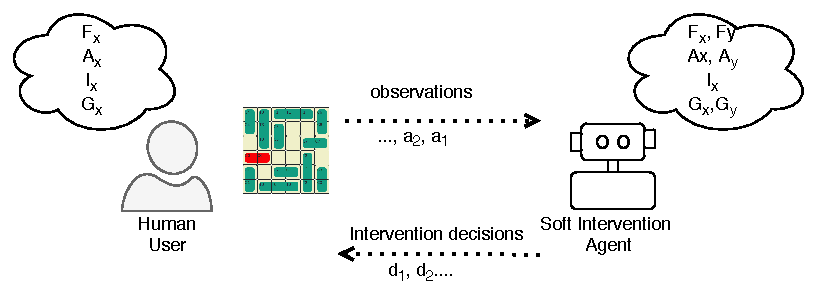
\includegraphics{img/model.pdf}
  \caption{The Soft Intervention Model}
  \label{fig:model}
\end{figure}
The planning problem for the soft intervention model develops around two actors: the human user and the intervention agent. As illustrated in Figure \ref{fig:model}, the human user's planning task is defined as: $\Pi_{user}=\langle F_x, A_x, I_x, G_x\rangle$, where $F_x$ is grounded with objects $\mathcal{O}\setminus o_f$, and $A_x \subseteq A_d$. $I_x$ is the initial board configuration and grounded with $\mathcal{O}$, which means the forbidden object is also available in the user's domain model. $G_x$ is the goal specification where predicates corresponding to car $C0$ being at the exit become \textit{True} in the state. User's solution to $\Pi_{user}$ generates an action sequence $\lbrace a_1, a_2, \ldots \rbrace$, which corresponds to the user's plan $\pi_{user}$. The intervention agent's domain model is different from the human user's because the agent knows about $o_f$. The intervention agent's planning task is defined as: $\Pi_{agent}=\langle \lbrace F_x\cup F_y\rbrace, \lbrace A_x \cup A_y\rbrace, I_x, (G_x\otimes G_y)\rangle$ where $F_x, A_x, I_x, G_x$ are defined as before. $F_y$ is grounded with $o_f$, and $A_y \subseteq A_u$. $G_y\subset F_y$ is the undesirable state. The agent's solution to $\Pi_{agent}$ is a plan $\pi_{agent}$. We use $\otimes$ symbol to denote that the agent needs to solve the planning problem for $G_x$, which \textit{avoids} $G_y$. In other words, any sub-plan (i.e, a sub sequence of actions) in $\pi_{agent}$ must not reach the state $G_y$.

User's actions have a cost that assigns a non-negative value to the action schema defined in the STRIPS domain definition. The cost function is given as $C: Op \rightarrow \mathbb{R}^0_+$. The cost of user's plan $c(\pi_{user})$ is  $\sum(c(a_i))$. The optimal solution, the optimal plan $\pi^*_{user}$, minimizes the cost. In this work, we assume all actions are uniform cost equal to 1.

When the user and the agent interact in real life, if the agent were to solve $\Pi_{agent}$, it would rely on an automated planner, which uses a variety of heuristics and optimizations. Because of this, a solution (or set of solutions) obtained by an automated planner may not match with the plan the user is producing. In intervention model we are proposing, the agent's role is to guide the user toward the goal and not directly solve the puzzle on the user's behalf. To do this, the agent needs to evaluate the user's plan up to now (a partial plan) to identify future problems. Our intervention design requires the agent to receive the user's actions as observations one at a time. Then the agent makes the decision to intervene having considered behavior properties of all observations made up to the current point. Our soft intervention model learns to recognize partial plans that may become unsafe in the future using these behavior properties. When the user makes a move on the puzzle, the intervention agent looks $k$ steps ahead into the future ($k \in \lbrace1,2,3\rbrace$) and decides whether or not the user will reach the undesirable state at step $k$. If the decision is yes, intervention takes place in the current step.
 
\subsubsection*{Assumptions About the Domain}
For the learned models developed from the results of this study, we make the following assumptions about the human user's planning problem for the Rush Hour domain.
\begin{description}
\item [User wants to avoid the undesirable state:]
In the scenarios we are modeling in this study, the need for intervention occurs when there is a mismatch between the human user's knowledge of the domain and the intervening agent's knowledge, and this discrepancy leads the user to an undesirable consequence. In the case of the Rush Hour domain, the user not being aware of the forbidden car creates an opportunity for the user to inadvertently commit to solutions that triggers the undesirable consequence. In the Rush Hour domain, we assume that the user does not behave as an adversary and attempt to willingly trigger the undesirable state. The adversarial case, in which  the environment contains an opponent (human/software agent) in addition to the human user and the intervention agent, is an interesting extension to the intervention problem and is applicable in many real-life domains such as cyber security and multi-player games.
\item [Knowledge of $G_x, G_y$:] 
We assume that the user is aware of the goal of the puzzle (i.e, move the red car to the exit) $G_x$ and actively pursues the goal. The user also welcomes the intervention decisions generated by the intervention agent. The user does not know the undesirable state $G_y$ but has the knowledge that it exists. The agent knows both $G_x$ and $G_y$.
\item [Actions are Deterministic and discrete:]
We assume that each action the user executes has only one outcome. The effect of the action is a discrete and instantaneous update of the state (vehicle positions) on the board.
\item [Observability:]
We assume that the user's actions (puzzle moves) are fully observable to the intervening agent.
\end{description}

\section*{The Rush Hour Web Simulator}
\subsection*{System Design Decisions}
We designed the Rush Hour software framework for conducting human subject studies in an environment that allows the user to be engaged in a cognitively taxing task. Our first design choice was in establishing the physical setup of the system. Because the experiments are targeted toward all kinds of computer software users (experts/non-experts), we wanted the subjects' attention to be mainly on the puzzle solving task and not be distracted by a complex user-interface. To allow for more users to participate, while minimizing the time commitment and the effort, we wanted the system to be accessible from anywhere (e.g, home, university etc.). Because of these reasons we designed the system to be a single page web application.
Our next design decision is concerned with capturing and storing experiment data. As per the university Institutional Review Board (IRB) regulations, the subject data is required to be stored in a secure manner. Further, because our system is deployed as a web application, multiple users may use the system at once and we need to ensure the data is transferred from the web application client to the server securely. We established communication between the client and the server over HTTPS via a stateless request-response scheme. The client side uses NodeJS, an asynchronous, event-driven JavaScript run-time, which is designed to build scalable network applications.  The client also uses NodeJS security modules (Helmet) for improved security. The data is stored in a secure remote, server dedicated to the web application. The design of the system needs to facilitate seamless transition between the two operating modes: learning behavior patterns that can be used as indicators of users' needing help and evaluating learned intervention models in situ. Therefore,  we designed the web application to interact with micro-services via a RESTful API. Our system architecture is RESTful, in the sense that the client interacts with the server by sending HTTP GET and POST requests using JSON messages to an endpoint URL in the server. The API defines many services (persisting game state, intervention, providing hints etc.). These services are implemented as separate components on the server. REST API response payloads sent from the server are text and encoded in JSON. The response is parsed at the client and appropriate event is triggered on the user interface. In addition to supporting platform-independence, which encourages user participation, the services can be activated and deactivated based on the operational mode. This allows us to extend the existing system to evaluate how human users respond different intervention models in the future.

\subsection*{System Architecture}
The basic system architecture is a JavaScript single page web application in an HTML5 browser that uses RESTful API to access micro-services provided by a Java server running on Linux. The client consists of a minimal index.html file that loads and executes the bundled JavaScript application. The client and server files are bundled into a single JAR file for the execution on the Linux server at a specified port. Figure \ref{fig:architecture} illustrates the system architecture.

\begin{figure}[!ht]
  \centering
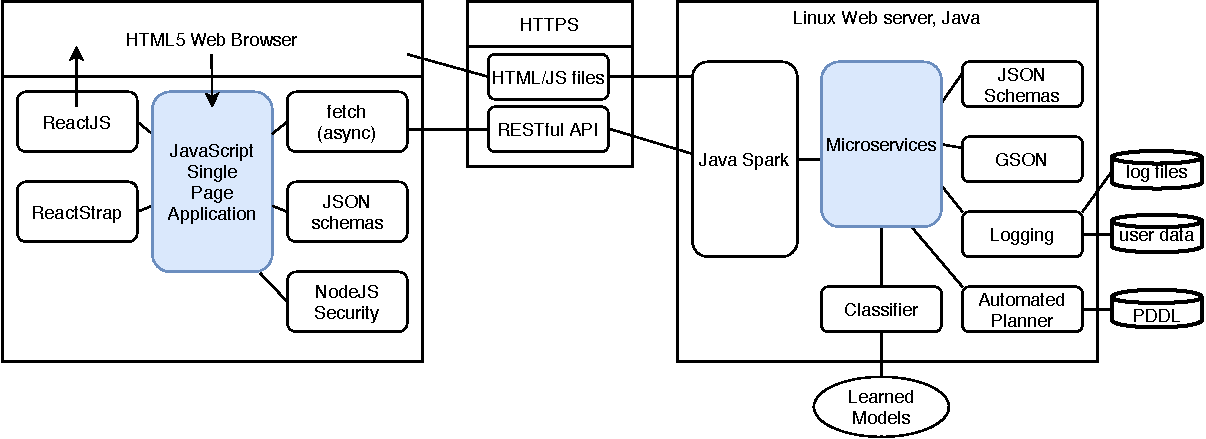
\includegraphics[width=\columnwidth]{img/architecture.pdf}
  \caption{The Client-Server Architecture of the Intervention System}
  \label{fig:architecture}
\end{figure}
The system is a client-server application that communicates over HTTPS. On the client side, the browser loads the index.html file, which in turn loads the bundled JavaScript single page application bundle.js. The single page application makes RESTful API requests to the server on the same port using JavaScript's asynchronous fetch. We defined several JSON schema to enable message passing between the client and the server via the RESTful API. The JSON schema verify requests on the server side and responses on the client side. Any verification failures are handled by error responses, also defined in the JSON schema. ReactJS renders the application using ReactStrap on the client. Because the communication between the client and the server occurs over the Internet, we use the NodeJS security module Helmet to secure the HTTP headers to prevent attacks like cross-site scripting.

On the server side, GSON is used to convert the JSON requests from the client to Java objects and Java objects to JSON responses. The server uses Java logging to record user data (moves, survey responses on the client side) and errors that occur on the server side on text files. The classifier and the automated planner components are activated only when evaluating learned intervention models. The automated planner component uses PDDL problem and domain definitions to retrieve information about the planning problem to help guide the user. The classifier component uses machine learning models to decide whether the user's partial solution requires intervention or not.

In the first mode of the operation, the application allows the user to solve the puzzle without any intervention. In this mode, the user interacts with four components: (1) consent agreement, (2) Rush Hour Tutorial, (3) Solver (Board), and (4) Post-study survey/Debriefing. The components are displayed as tabs on the web page. As the subject interacts with each of these components, unique API calls are triggered to inform the server about the status of the game. The consent agreement component lets the subject read the terms and conditions of the study and give informed consent to participate in the study as required by the IRB. When the user gives consent to participate in the study, the user gets assigned a unique identifier and components 2 and 3 get activated. This unique identifier is maintained at both the client side (as the Local Storage entry in the Web browser) and on a text file at the server until the user's session ends. The Rush Hour tutorial presents a brief introduction to the Rush Hour puzzle, the rules and the objective of the puzzle. It also shows an example play to educate the user on how to select and move objects on the web interface. Components 1 and 2 are static components, in the sense the user does not have a lot of flexibility to change the contents through interaction. On the other hand, the solver is a dynamic and an interactive component. The solver component allows the user to start a puzzle solving task by clicking a button, at which point a random Rush Hour puzzle is fetched from the server. The participant can move the vehicles on the grid by first clicking once on the vehicle to select it and then clicking once on an adjacent empty cell to move it to the selected cell. To comply with the classical planning model of discrete actions, the application forces the user to move the vehicles one step at a time. This rule invalidates moves that jump over multiple cells on the puzzle boards. The other illegal move is user attempting to move a vehicle in the opposite orientation. When the user makes one of these illegal moves, error messages are displayed and the move is blocked. All legal moves the user make are temporarily kept in in-memory data structures on the client side. Once the user finishes the puzzle solving task, an API call is invoked to initiate the data transmission between the client and the server in a secure manner via HTTPS. The server records the users solution on a text file in a directory created with the user's identifier. When the user's solution is stored on the server successfully, component 4 gets activated. The post-study survey in this mode, collects demographic data and the user's general puzzle solving habits. Once the user completes the survey, the data is transmitted to the server to be stored similar to the data storage protocol used in component 3.

\begin{figure}[!hbt]
  \centering
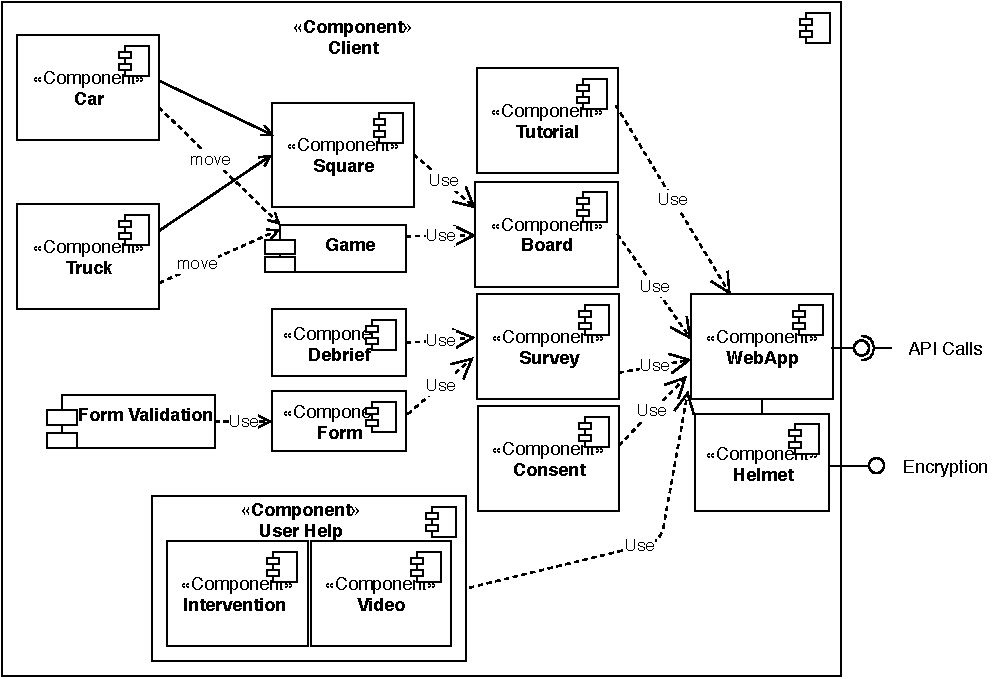
\includegraphics[width=\columnwidth]{img/componentclient.pdf}
  \caption{UML Component Diagram for the Intervention System Client}
  \label{fig:compclient}
\end{figure}

Figure \ref{fig:compclient} illustrates the component structure of the intervention client used in the second mode of operation, which uses intervention. In this mode, the user interacts with five components on the client side: (1) consent agreement, (2) Rush Hour Tutorial, (3) Solver, (4) User Help and (4) Post-study survey/Debriefing. Components 1, 2, 3, and 5 function similar to the first operation mode. The User Help component is used to communicate intervention decisions from the server and the subsequent user responses. In this study we evaluate the effects of offering help before the user starts the puzzle solving task and during. Video component supports the former, which plays a 45 second video clip on how to solve an example puzzle. The video is played to randomly selected users to simulate an experiment condition. The intervention component supports intervention decisions during the play. The communication model between the client and the server differ from the first operation mode, in that in addition to retaining users' moves in memory, each puzzle move the user makes invokes an API call to the server to retrieve an intervention decision. If intervention occurs, the Intervention component displays a pop-up dialog box with five help options. When the user requests one of the help options, the client makes another API call to fetch a response from the server. The response is displayed as a follow up dialog box and the user is allowed to continue on with the puzzle solving task. Figure \ref{fig:help} shows the intervention message shown to the user (left) and  the user requesting to see the next best move and the subsequent response from the server displayed for the user (right). One of the help options is to let the user ignore intervention. The intervention component keeps track of how many times the user has chosen to ignore intervention and after two consecutive ignore requests, the client terminates fetching intervention responses from the server. When the puzzle solving task finishes, the user's solution and different responses to intervention decisions are transmitted to the server for persistence.

\begin{figure}[!hbt]
  \centering
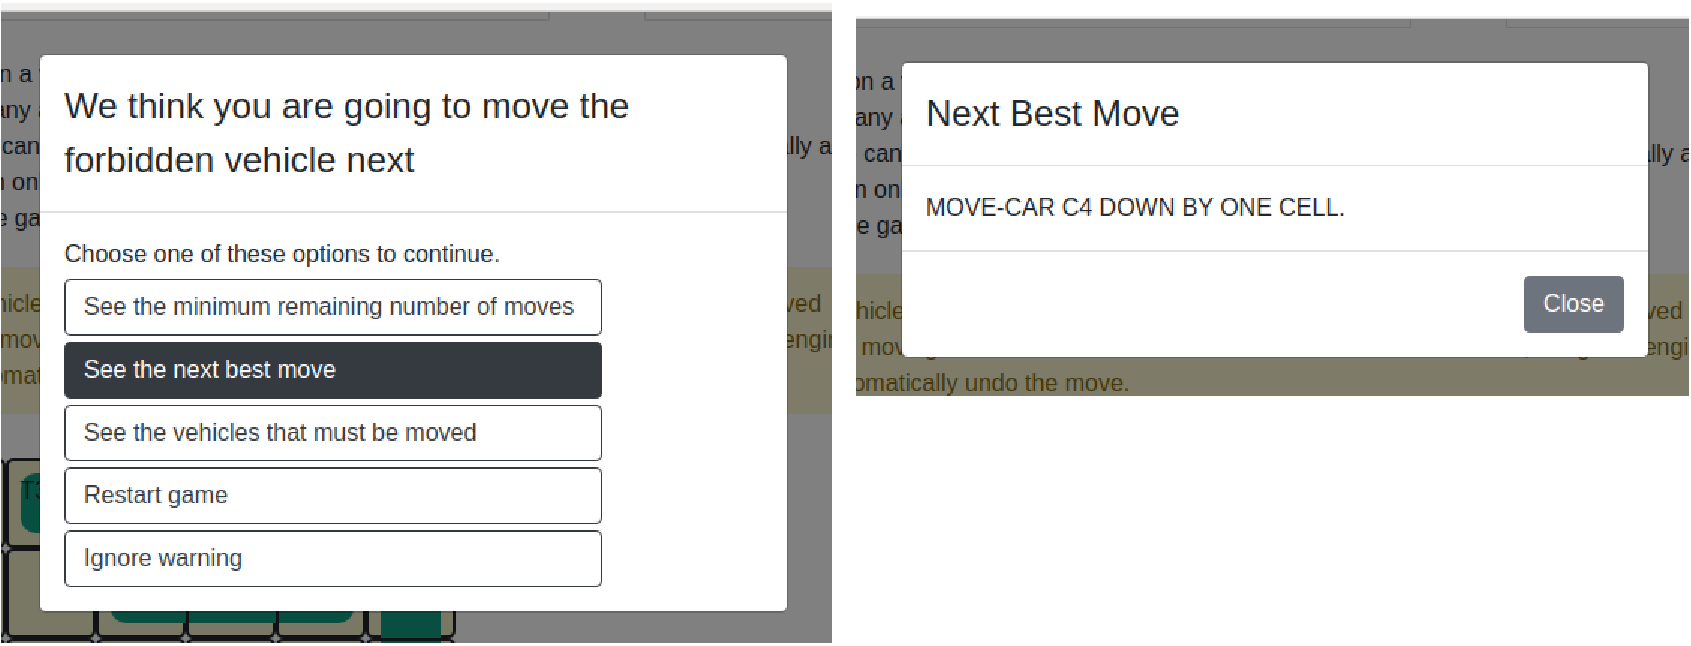
\includegraphics[width=\columnwidth]{img/alert.pdf}
  \caption{Intervention Step and Help}
  \label{fig:help}
\end{figure}
As shown in Figure \ref{fig:compserver}, the server responds to client's API calls through the micro-server. The intervention component and the planning component in the server are used to identify when the user needs help and generate helpful hints respectively. The intervention component uses a classifier to identify behavior features in the user's solution. The planning component responds to user's responses to intervention decisions by generating optimal plans and landmarks for the Rush Hour planning problem.

\begin{figure}[!hbt]
  \centering
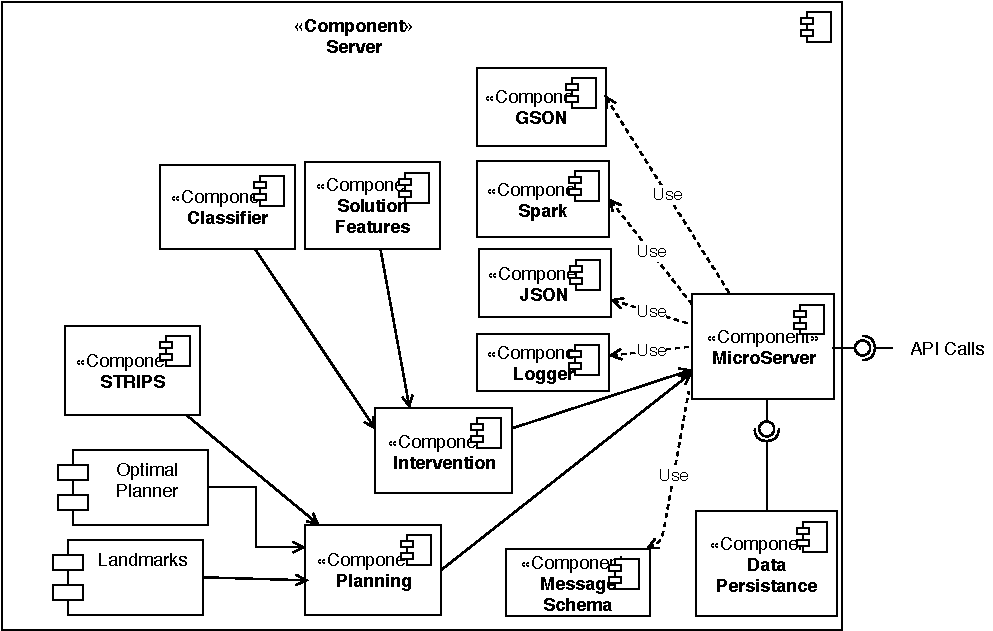
\includegraphics[width=\columnwidth]{img/componentserver.pdf}
  \caption{UML Component Diagram for the Intervention System Server}
  \label{fig:compserver}
\end{figure}

We use a minimalist and responsive design (supported by ReactStrap library) for the web application interface to help the user to start the puzzle solving task with a very small learning curve. The simple interaction model we designed for the users' to solve the puzzle and simultaneously communicate event data to the server helps the user focus completely on the puzzle solving task. The system is launched on a secure Linux web server with a public IP address, which allows the users to access the application from anywhere on a variety of devices. Figure \ref{fig:ui} shows the web application interface: the tutorial tab, play tab before the user starts the puzzle and when the puzzle is loaded in that order.
\begin{figure}[!hbt]
  \centering
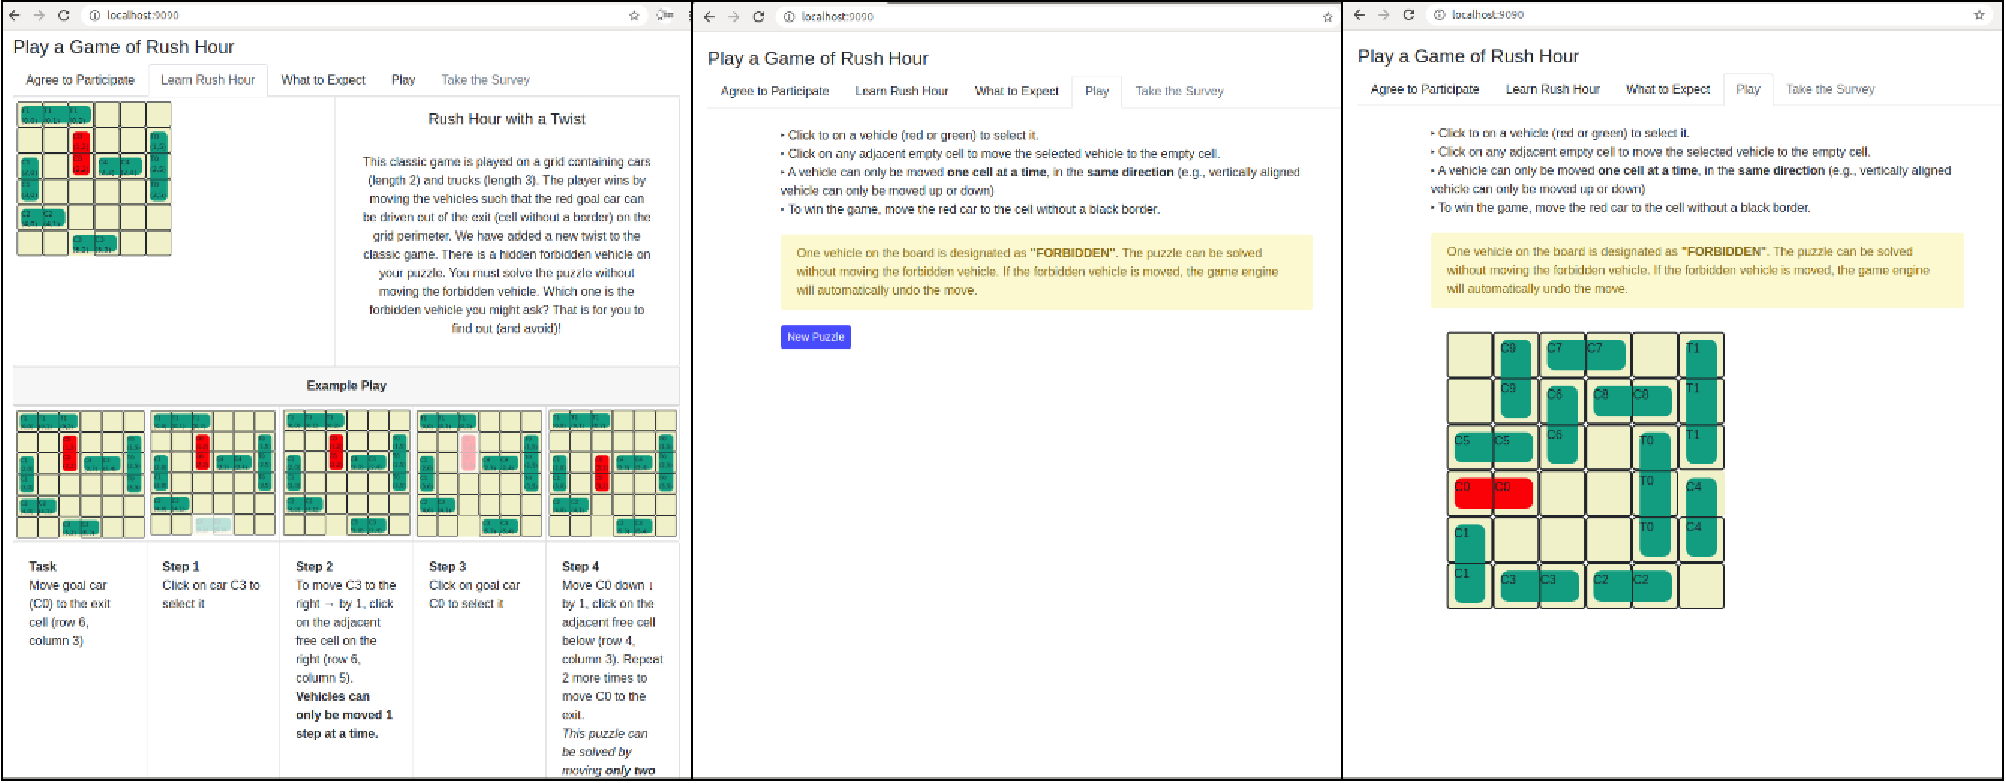
\includegraphics[width=\columnwidth]{img/UI.pdf}
  \caption{Rush Hour Simulation Framework Web Interface}
  \label{fig:ui}
\end{figure}
\subsection*{Rush Hour Puzzle Design Decisions}

When choosing Rush Hour puzzle configurations for the study, we want to carefully balance the puzzle's difficulty for a human user. Especially, given the PSPACE-completeness of the (generalized) puzzle, we need the puzzles to be solvable by human users in a reasonable time. Further, we use the Rush Hour puzzle as a supplementary task comparable to human users learning to use a new software or a web application. Therefore, the puzzle solving task should pose a sufficient challenge for the user during the search for a solution in order to make the intervention step more meaningful. We introduce a forbidden vehicle, which must not be moved to each puzzle to restrict the moves the user is allowed to make. This is an alternative way to increase the difficulty of the puzzle without having to increase the number of vehicles on the board \cite{fernau2003}. In order to further instill the importance of avoiding the forbidden vehicle in the user's mind, we also provided warning messages on the Web interface (see the yellow information bar in Figure \ref{fig:ui} panel 2/3) to inform the user about the presence of a forbidden vehicle and what will happen should the forbidden car was moved. However, the users are not explicitly informed what the specific forbidden vehicle is, unless the user moves it during game play. At that point, the user is first shown an alert message indicating that the forbidden vehicle was moved and the move will be undone.

In this study we use ten Rush Hour puzzles to produce learned models for soft intervention and three additional puzzles to evaluate the helpful hints. We classify these thirteen puzzles into three groups by the position of the forbidden vehicle. Figure \ref{fig:puzzles} shows the three puzzle types: type A has the forbidden vehicle in the corner of a grid, type B has the forbidden vehicle on the edge of the grid and type C has the forbidden vehicle in the middle of the grid. We hypothesize that these three types will pose unique challenges for the user to avoid the forbidden vehicle. To produce the learned models, we use four puzzles of type A, five puzzles of type B and one puzzle of type C. To evaluate helpful hints, we use four puzzles from types A, C and five puzzles from type B. Table \ref{tab:puzzles} shows the puzzle assignments used to produce learned models (10 puzzles) and evaluate hints (13 puzzles). $Pi, i=\lbrace 1,\ldots,13 \rbrace$ indicate the puzzle identifier.

\begin{figure}[!hbt]
  \centering
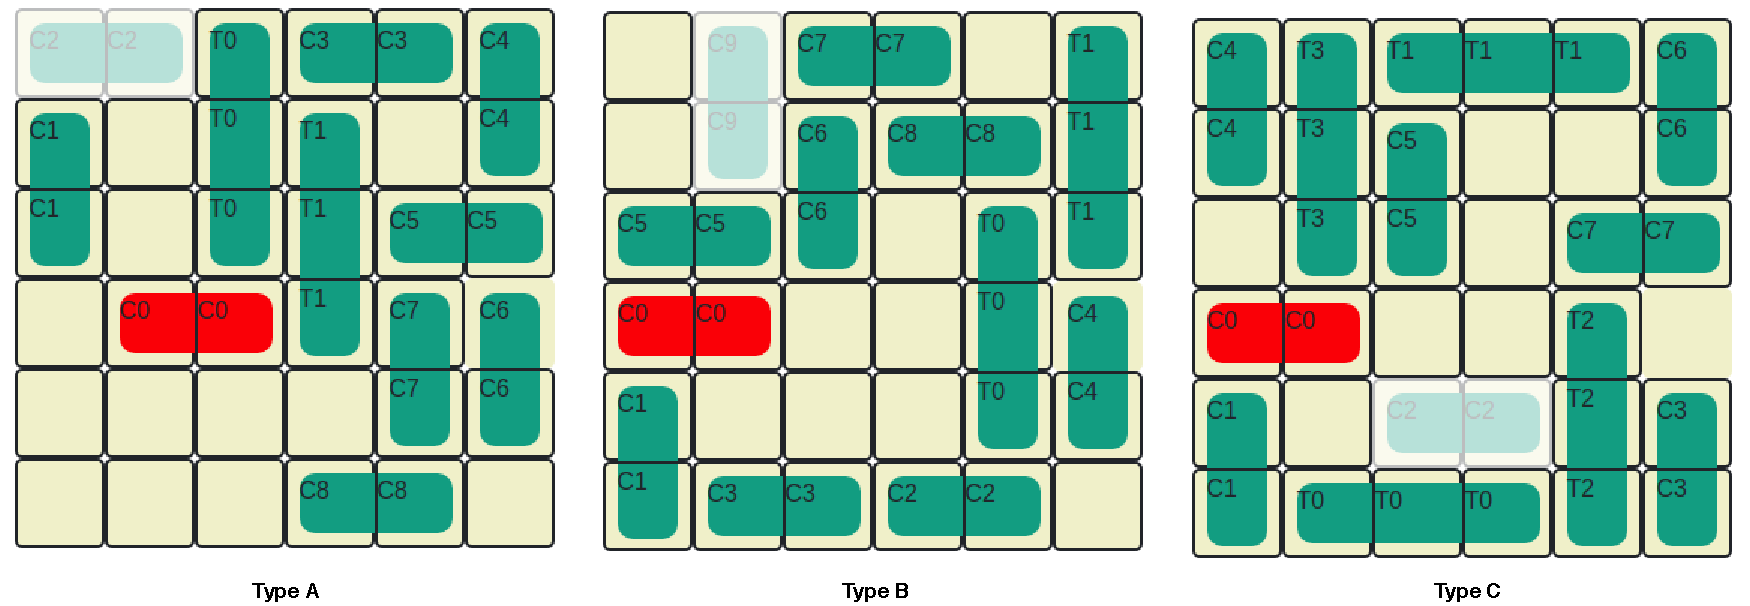
\includegraphics[width=\columnwidth]{img/puzzles.pdf}
  \caption{Rush Hour puzzle configuration types with forbidden vehicles highlighted}
  \label{fig:puzzles}
\end{figure}

\begin{center}
\begin{table}
\begin{tabular}{ll}
\begin{tabular}{|c|c|}
\hline
Type & Puzzles\\
\hline
A & P2, P4, P6, P8 \\
\hline
B & P1, P3, P5, P9, P10 \\
\hline
C & P7 \\
\hline
\end{tabular}
\quad
\begin{tabular}{|c|c|}
\hline
Type & Puzzles\\
\hline
A & P2, P4, P6, P8 \\
\hline
B & P1, P3, P5, P9, P10 \\
\hline
C & P7, P11, P12, P13 \\
\hline
\end{tabular}
\end{tabular}
\caption{Rush Hour puzzle assignment for learning intervention (left) and evaluating hints (right)}\label{tab:puzzles}
\end{table}
\end{center}

\section*{Learning Soft Intervention} %Phase 1
When the user solves a puzzle, the intervening agent receives the vehicle moves as a series of observations $\mathcal{M}=\lbrace m_1, m_2, \ldots \rbrace$, and $\mathcal{M} \subseteq \mathcal{A}$. Given $\mathcal{M}$, an initial state $I$, puzzle goal state $G_x$, and an undesirable state to avoid $G_y$, the soft intervention problem is defined as a tuple $\Xi=\lbrace \mathcal{M}, I, G_x, G_y\rbrace$. Execution of $\mathcal{M}$ is defined using the state transition function $\delta$ recursively as follows:

\begin{definition}
The execution of a sequence of linearly ordered actions $\mathcal{M}$ of length $l$ ($|\mathcal{M}|=l$) from the initial state $I$ results in a state $s$ defined by the function: $\Delta (I, \mathcal{M}) = \delta( \ldots \delta(\:\delta(I,m_1),\:m_2) \ldots, m_l)$
\end{definition}

Note that $\mathcal{M}$ is only a partial solution for the puzzle solving task $\Pi_{user}$ and $\Delta (I, \mathcal{M}) \not\models G_x$. The intervening agent needs to decide to intervene or not for a partial solution $\mathcal{M}^F, |\mathcal{M}^F|=k$ and $k>l$. In other words, the agent predicts whether or not the user will reach $G_y$, ($k-l$) steps into the future. For this work we restrict the interval of $(k-l)=[1,3]$. Therefore, we represent the \textit{soft intervention problem} for the Rush Hour puzzle as a binary classification problem. Formally, the solution to the soft intervention problem is a function $\mathcal{I}$ such that, given a $N$-dimensional input vector $x \in \mathcal{X} \subseteq \mathbb{R}^N$, $x$ is mapped to a set of fixed classes $C$:

\begin{equation}
\mathcal{I} : \mathcal{X} \to C=\lbrace Yes, No\rbrace
\end{equation}

The label \textit{Yes} indicates that the human user needs help and must be intervened, while the \textit{No} label indicates that the human user should not be intervened. In the supervised mode, $\mathcal{I}$ is learned by observing actual examples of human users solving Rush Hour puzzles. We denote the supervised learning method by $T$ and $T(D)=\mathcal{I}$. The learning method $T$ takes a training set $D$ as input and returns the learned classifier function $\mathcal{I}$. We explore five learning methods in this study: $\mathcal{I} \in \lbrace $ Decision Tree, Random Forest, k-nearest neighbor, Logistic Regression, Naive Bayes $\rbrace$  $D$ is a set of labeled game plays $\langle g, c\rangle$ where $\langle g, c\rangle$ $\in X \times C$. 

We want to transform the user's game play $g$ into a representation of $x$ that allows us to capture where the user is in the state space of the Rush Hour planning problem at the time the decision to intervene is made and  produce measurable attributes that describe how the user has been exploring the state space. For example, is the user advancing toward the winning state by making helpful moves?, is the user currently exploring a risky part in the state space and getting closer to the undesirable state? We hypothesize that behavior patterns as these have a correlation to the event of the user moving the forbidden vehicle and these patterns can be used to as features of a learning method to recognize in advance if the user needs intervention. We designed a human subject experiment to identify common behavior patterns.

\subsection*{The Human Subject Experiment}
\subsubsection*{Experimental Design}
As shown in Table \ref{tab:puzzles}, we created ten unique Rush Hour puzzles. We conducted a pilot study using nine graduate students to assess whether the human solvers were able to solve the selected puzzles within a reasonable amount of time. The pilot study participants solved their assigned puzzles within 5 - 10 minutes. The pilot study participants were also interviewed informally to get their perception of the puzzle difficulty. The participants commented that the puzzles were ''\textit{challenging}'' and "\textit{forced me to think}". The same puzzles used in the pilot were used in the actual study.

For the actual study, we recruited subjects from a graduate and undergraduate university student population. The participants were not compensated for their time. After obtaining informed consent, the participants were directed to the Web URL, which hosted the Rush Hour simulator software. Each participant was assigned to solve one Rush Hour puzzle randomly selected from a set of ten. We did not place any time restriction for the puzzle solving task. Participants also had the option to use an online tutorial (available on the simulator itself) on how to play the Rush Hour puzzle. All ten puzzles contained a forbidden vehicle. Participants were informed that one of the vehicles on the game board is forbidden and the puzzle must be solved without moving the forbidden vehicle. However, in this phase we did not give any visual cues (error messages, blocks) to the user in case they happen to move the forbidden vehicle during game play. Once the puzzle solving task was completed, the participants were asked to complete a short demographic survey on their general puzzle solving habits. Figure \ref{fig:phase1} illustrates the activity sequence of the experiment. 136 participants completed the study. The sample comprised of college undergraduate and graduate students in Computer Science, Psychology, Agriculture and Business majors. 117 of the 136 participants also completed the demographics survey.

\begin{figure}[!hbt]
  \centering                                                    
  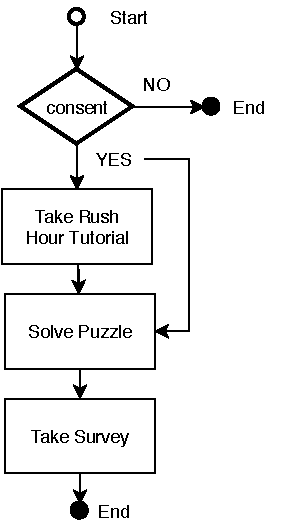
\includegraphics[keepaspectratio]{img/phase1.pdf}
  \caption{Activity sequence for learning when to intervene human subject experiment}
  \label{fig:phase1}
\end{figure}

\subsubsection*{Findings - Demography Survey}
Majority of the participants (39) were below the age of 20, while 38 subjects were between the age 20-25. Maximum age was 41 years. 70 of the 117 participants were male. When asked if they liked puzzle solving tasks, 78\% of the participants either agreed or strongly agreed with the statement. Specifically to the Rush Hour game 79\% of the participants liked or strongly liked Rush Hour. The most common reason as to why the participants liked puzzle solving tasks was that puzzle solving stimulates critical thinking skills. 30\% of the participants usually did a puzzle solving task once a month, while 21\% of the participants solved a puzzle once a week.

When asked about strategies the participants used to solve difficult puzzles, 79\% of the group said that they kept trying until the puzzle was eventually solved, while 12\% of the participants said that they would ask for help. 

Given a new puzzle that they have not seen before, if they get stuck while solving the puzzle, 26\% said that they would not like any outside help. 47\% of the participants said that they would like a suggestion/tip that would get them past the current situation. 15\% said that they would like a warning, which indicated that their current approach would lead to a dead-end. 8\% of the participants said that they would like a warning and an explanation to help them prevent getting stuck in the future.  The most common medium for solving puzzles was using their mobile devices (42\%). 31\% of the participants used the personal computers/laptops to solve puzzles. 19\% of the participants solved puzzles using physical means (e.g., puzzle books, newspapers and physical puzzles such as Rubik's  cubes)

\subsubsection*{Findings - Avoiding Forbidden Vehicle}
The Rush Hour search problem can be optimized using two parameters: (1) number of moves and, (2) number of vehicles moved. Defining the Rush Hour problem as a STRIPS planning problem allows us to use off-the-shelf planners (configured to use an admissible heuristic during search) to find solutions optimized to minimize both these parameters. Regardless the optimizing parameter, inclusion of the forbidden vehicle further classifies the optimal solutions into two categories: (1) safe - optimal solutions that do not contain forbidden vehicle moves and (2) unsafe - optimal solutions that contain forbidden vehicles moves. Optimal solution costs for all these categories of solutions are summarized in Table \ref{tab:optimals}. It can be seen that solution costs for safe and unsafe solutions for the ten puzzles optimizing for the minimum number of vehicles is identical. However, optimizing for the minimum number of moves we see that for puzzles P3 and P5, the unsafe solution costs less than the safe solution. This means that it is possible for the user to find a shorter solution for these two puzzles by moving the forbidden car. We used the HSP planner \cite{bonet01planningas} to find the optimal solutions.

\begin{table}[!htb]
\begin{tabular}{|l|c|c|c|c|}
\hline
\multirow{2}{*}{PID} & \multicolumn{2}{l|}{Number of Moves} & \multicolumn{2}{l|}{Number of Cars} \\ \cline{2-5} 
    & Safe & Unsafe & Safe & Unsafe \\ \hline
P1  & 24   & 24     & 8    & 8      \\ 
P2  & 30   & 30     & 10   & 10     \\ 
P3  & \textbf{35}   & \textbf{25}     & 10   & 10     \\ 
P4  & 23   & 23     & 9    & 9      \\ 
P5  & \textbf{21}   & \textbf{14}     & 7    & 7      \\ 
P6  & 22   & 22     & 8    & 8      \\ 
P7  & 21   & 21     & 8    & 8      \\ 
P8  & 9    & 9      & 5    & 5      \\ 
P9  & 21   & 21     & 10   & 10     \\
P10 & 24   & 24     & 9    & 9      \\ \hline
\end{tabular}
\caption{Optimal costs for the safe and unsafe Rush Hour solutions for puzzles P1 through P10, optimized for number of moves and number of cars}
\label{tab:optimals}
\end{table}

From the 136 subjects, 66 produced solutions that involved moving the forbidden vehicle. From those who moved the forbidden vehicle, 54 users moved the vehicle more than once. Mean number of moves was 53 ($SD=55$) for the sample and maximum number of moves was 378. Table \ref{tab:usersolutions} describes the summary statistics for safe and unsafe solutions produced by the human solvers. Figure \ref{fig:split} illustrates the percentage split between unsafe and safe solutions for each puzzle. All users who solved P1 (type A), P6 and P8 (both type B) avoided the undesirable state. Interestingly, examining the structure of P1, although it is type B, it can be seen that moving the forbidden vehicle makes the puzzle unsolvable. The users who solved P1 did not move the forbidden vehicle. 

\begin{figure}[htb]
  \centering
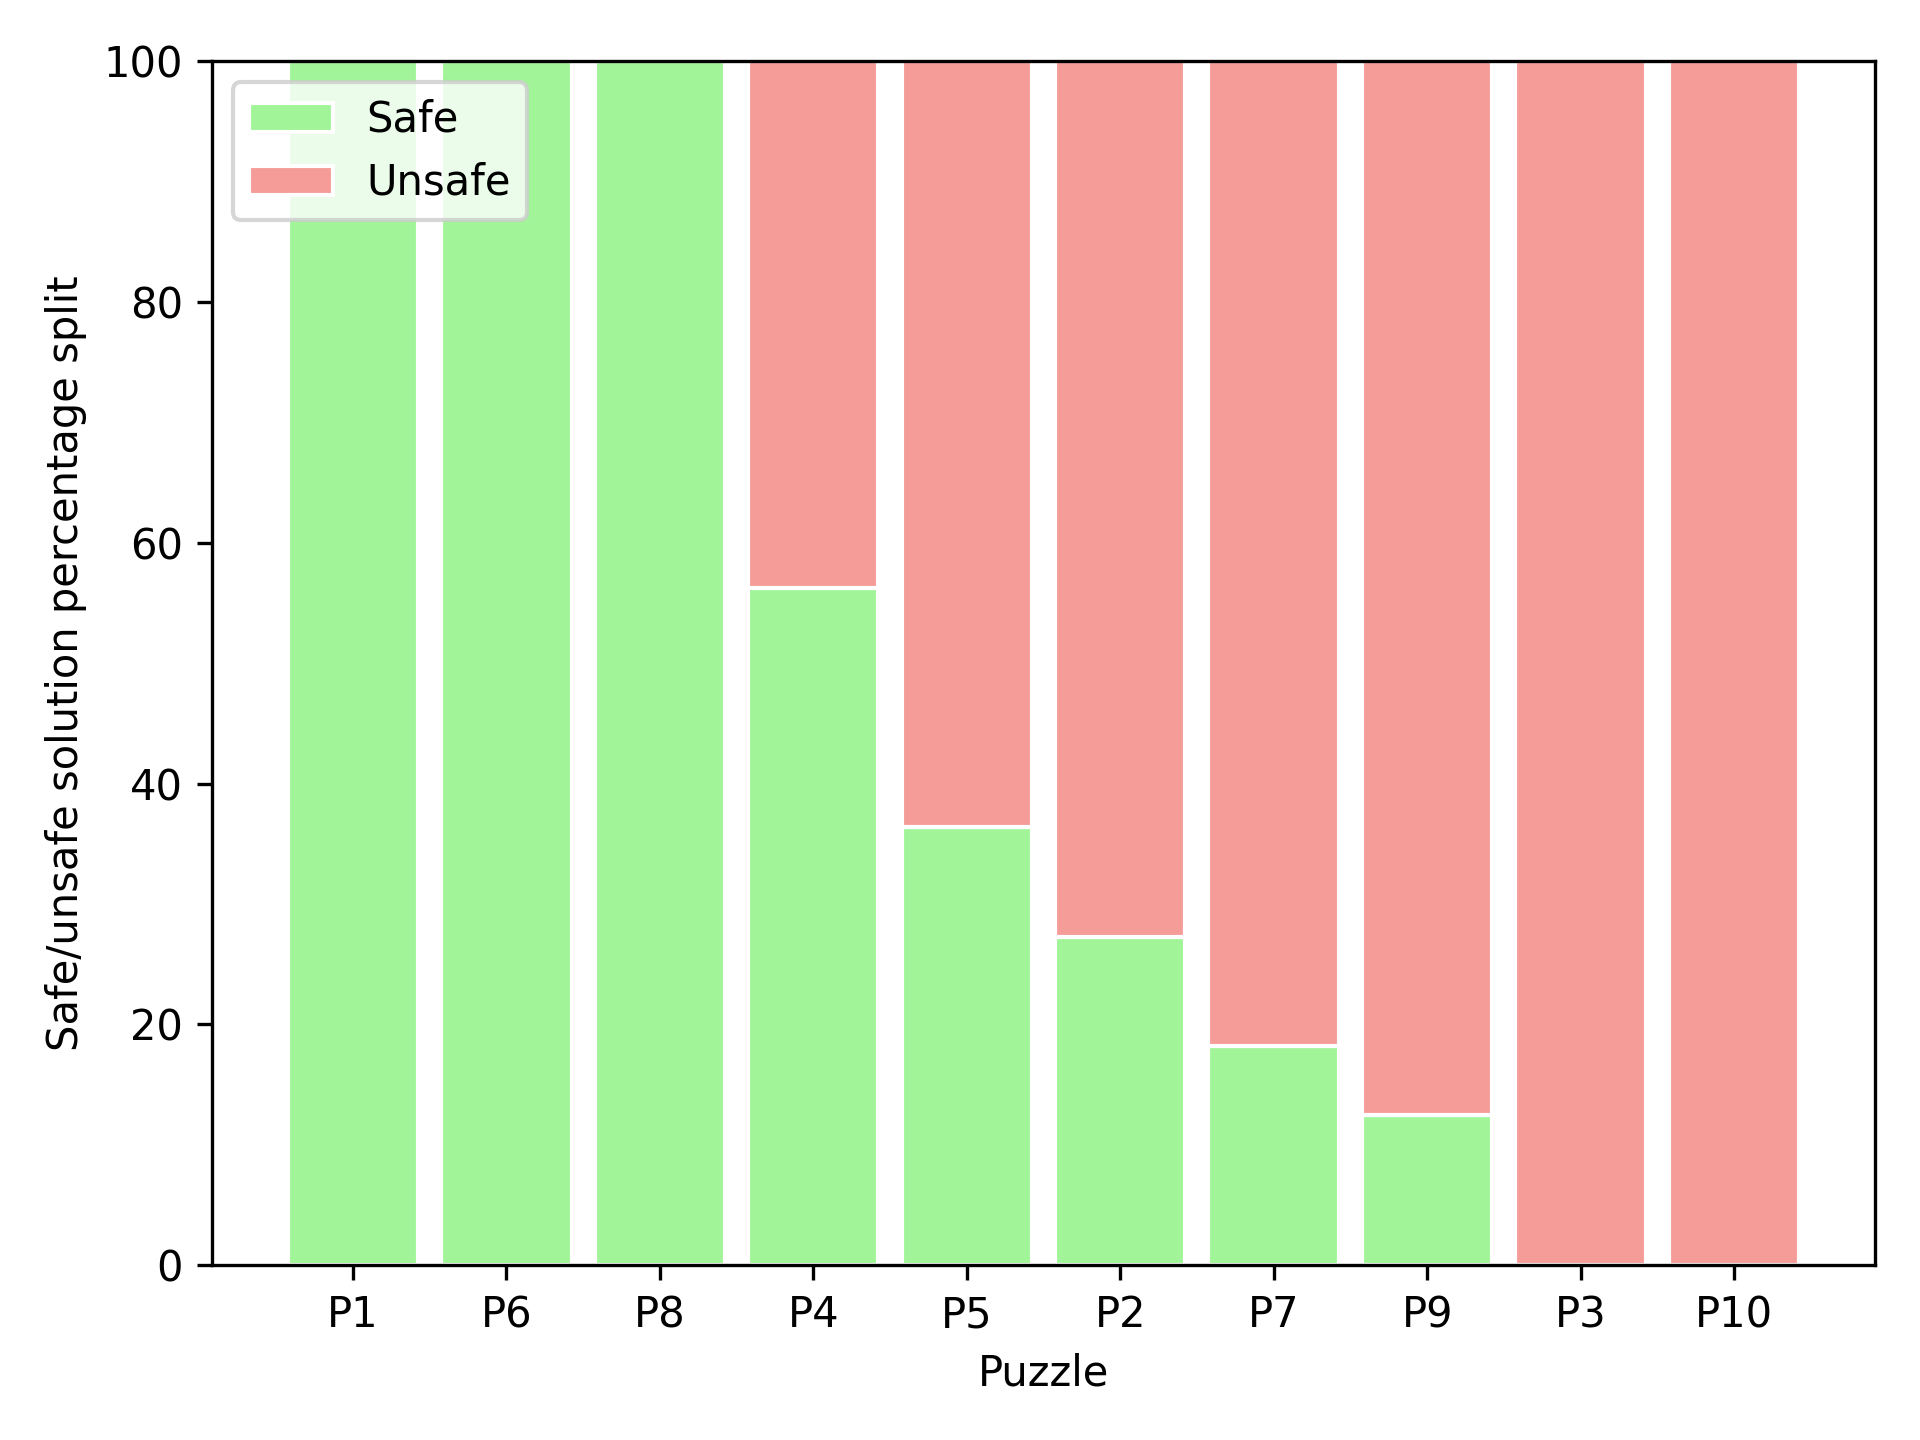
\includegraphics[width=0.5\columnwidth]{img/p2.png}
  \caption{Percentage split between unsafe and safe solutions produced by human users for puzzles P1 through P10}
  \label{fig:split}
\end{figure}
\begin{table}[htb]
\begin{tabular}{|l|l|l|l|l|l|l|l|l|l|l|}
\hline
\multicolumn{1}{|c|}{\multirow{2}{*}{PID}} &
  \multicolumn{5}{c|}{Safe Solutions} &
  \multicolumn{5}{c|}{Unsafe Solutions} \\ \cline{2-11} 
\multicolumn{1}{|c|}{} &
  \multicolumn{1}{c|}{Freq} &
  \multicolumn{1}{c|}{Min} &
  \multicolumn{1}{c|}{Max} &
  \multicolumn{1}{c|}{Mean} &
  \multicolumn{1}{c|}{SD} &
  \multicolumn{1}{c|}{Freq} &
  \multicolumn{1}{c|}{Min} &
  \multicolumn{1}{c|}{Max} &
  \multicolumn{1}{c|}{Mean} &
  \multicolumn{1}{c|}{SD} \\ \hline
P1  & 18 & 24 & 106 & 43.9  & 20.5  & -  & -  & -   & -    & -    \\ 
P2  &  3  & 44 & 158 & 99.3 & 57.1 & 8  & 78 & 378 & 190.3 & 120.0\\ 
P3  & -  & -  & -   & -     & -     & 12 & 25 & 50  & 35.5 & 8.3  \\ 
P4  & 9  & 23 & 46  & 30    & 7.1   & 7  & 25 & 124 & 67.4 & 33.9 \\ 
P5  & 4  & 23 & 32  & 26.5  & 3.9   & 7  & 14 & 82  & 32.0 & 23.3 \\
P6  & 14 & 22 & 55  & 29    & 10.3  & -  & -  & -   & -    & -    \\
P7  & 2  & 29 & 37  & 33    & 5.7   & 9  & 43 & 132 & 80.9 & 38.2 \\ 
P8  & 18 & 9  & 12  & 9.3   & 0.8   & -  & -  & -   & -    & -    \\
P9  & 2  & 21 & 27  & 24    & 4.2   & 14 & 29 & 169 & 66.3 & 39.0 \\
P10 & -  & -  & -   & -     & -     & 9  & 44 & 158 & 81.2 & 39.2 \\ \hline
\end{tabular}
\caption{Frequency, minimum, maximum, mean and std. deviation number of moves in users' solutions for the Rush Hour puzzles P1 through P10}
\label{tab:usersolutions}
\end{table}

\subsection*{Extracting Features}
We use the properties derived from the game state (positions of objects on the board) and the properties of the users' partial solution that has been observed up to now to extract features that correspond to the user's game play behavior. 
\subsubsection*{Game State}
We describe the game state using the \textit{vehicle positions} and  also their \textit{mobility}. With soft intervention, we hope to help the user reach the goal state, while avoiding the undesirable state. To this end, to learn the soft intervention model, instead of describing the positions of all the vehicles on the board, the features that capture the game state mainly focus on the positions of only the target vehicle (red color) and the forbidden vehicle and also their corresponding adjacent vehicles. We use the game state features associated with to the target car to measure how close the user is to the goal state. The features associated to the forbidden car evaluate how close the user is getting to triggering the undesirable state. Furthermore, we use a combination of raw feature values corresponding to the game state, as well as the abstractions of these features such as the mean and the frequency. This reduces the size of our input feature vector and at the same time gives us an estimate on where the user is in the state space; closer to moving the forbidden vehicle or advancing toward the goal state.

In general, the human solvers found it easier to avoid moving the forbidden vehicle in type A puzzles. Three of the four type A puzzles, had all or majority of human solvers managing to avoid the forbidden vehicle. Altogether, 83\% of subjects who solved type A puzzles avoided moving the forbidden vehicle. On the other hand, when the forbidden vehicle is on the perimeter of the board, type B, human solvers often moved the forbidden vehicle. In this case, only 36\% of the users who solved type B puzzles, managed to avoid moving the forbidden vehicle. All human solvers who attempted two puzzles of type B (P3, P10) moved the forbidden vehicle in their solutions. Ability to avoid moving the forbidden car dropped further for type C puzzles. The majority of the users (82\%) who attempted P7 (type C) moved the forbidden vehicle while solving the puzzle. This is intuitive because the forbidden vehicle in type C is the most exposed thus making the user less likely to correctly guess the forbidden car in advance.

Mobility of the two critical objects in the puzzle: target car and the forbidden vehicle, provide clues about the users' game state. As seen in the three puzzle types, more blocked the forbidden vehicle is the less likely the users are to move it. The objects on the path of the target car must first be moved out to clear the path. In doing so, the human user could move vehicles in such a way that the forbidden vehicle becomes free. In the initial configuration of the puzzles used for this experiment, the forbidden vehicles were blocked from all sides. Only puzzles P7 and P9 had the forbidden vehicles free in the initial configuration. We manually examined the human user solutions produced in this experiment to identify common movement patterns. We found that if the user was moving vehicles adjacent to the forbidden vehicle in such a way that the forbidden vehicle was freed, most users ended up moving it. This means that by monitoring the state changes that occur around the forbidden car, we can estimate whether the user will end up moving the forbidden vehicle or not. Similarly we capture the vehicle movements that take place on the target car's path to the exit, for example, the moves that result in reducing the number of vehicles blocking the target car is considered to be helpful to move the game state closer to the goal state.

Note that during a game play a human user can move the forbidden car multiple times because the simulator does not give any feedback in this experiment. When extracting features for the soft intervention model, we consider the partial solutions from the start to the point when the forbidden car was moved for the first time. In addition to the target and the forbidden vehicles, we introduce two additional critical vehicle sets: \textit{target car blockers} and \textit{forbidden car blockers}. Blockers are vehicles that are  directly on the path of another vehicle. Figure \ref{fig:blockers} illustrates an example board state. The target car's path is blocked by two vehicles C1 and T1. Therefore, \textit{target car blockers} $= \lbrace C1, T1\rbrace$. We only consider the vehicles that are between the target car and the exit cell as blockers because, only those vehicles are preventing the target car from reaching the goal state. The forbidden vehicle's movement is blocked by two vehicles C1 and C2. Therefore, \textit{forbidden car blockers} $=\lbrace C1, C2\rbrace$. We now describe the behavior features we designed considering the game state.

\begin{figure}[htb]
  \centering
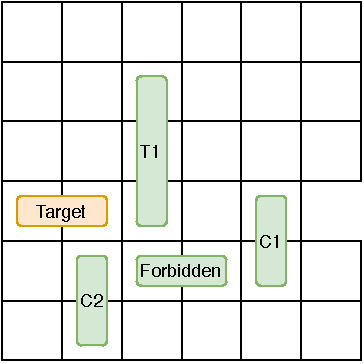
\includegraphics[width=0.35\columnwidth]{img/blockers.pdf}
  \caption{Blocker Vehicles}
  \label{fig:blockers}
\end{figure}
\begin{description}
\item[\texttt{blocks}:] number of times a move increased the number of cars blocking the target car's path
\item[\texttt{frees}:] number of times a move freed up empty spaces around the forbidden vehicle
\item[\texttt{freebci}:] number of times the number of empty spaces around the forbidden vehicle blockers increased
\item[\texttt{freebcd}:] number of times the number of empty spaces around the forbidden vehicle blockers decreased
\item[\texttt{freegci}:] number of times the number of empty spaces around the target car blockers increased
\item[\texttt{freegcd}:] number of times the number of empty spaces around around the target car blockers decreased
\item[\texttt{mgc}:] mean number of empty spaces around the target car blockers
\item[\texttt{mbc}:] mean number of empty spaces around the forbidden car blockers
\item[\texttt{reset}:] number of times the current move changed the state back to the initial puzzle configuration
\end{description}

\subsubsection*{Human Solvers' Partial Solutions}
The partial solutions the human users generate during game play provide clues to deciding whether or not the user will trigger the undesirable state. As seen in Table \ref{tab:usersolutions}, the mean number of moves for a safe solution (a solution that does not contain forbidden vehicle moves) is lower than the mean number of moves for an unsafe solution for the same puzzle. When we manually examined the human user solutions we found that the users who produced unsafe solutions often made unhelpful moves. For example, most of them moved the same vehicle back and forth many times in succession. For this study, we define one unhelpful move type called the \textit{h-step undo}.

\begin{definition}
Given a partial solution $\mathcal{M}=\lbrace m_1, m_2...m_i \rbrace$, $|\mathcal{M}|=i$, $\mathcal{M}\subseteq \mathcal{A}$ and initial state $I$, let state $s_i=\Delta(I,\mathcal{M})$. A h-step undo is a state transition such that $\Delta(s_i, \lbrace m_{i+1}, \ldots, m_h\rbrace)=s_i$ and $h>i$, $h \in \mathbb{N}$.
\end{definition}

The h-step undo is a move that takes the game state back to a previously seen state (i.e, an undo operation). In this work we only consider $h=1$, which asks the question did the current move just undo the move that happened immediately before?

Comparing the number of moves of the partial solution to that of an optimal solution is helpful in identifying whether the user is moving away from the goal state or making progress toward it. Here, we use the safe solution optimized for the number of moves. We used the HSP planner to find the optimal solution for each puzzle. Figure \ref{fig:difficuly} illustrates how the number of moves in users' solutions compare to a set of threshold values derived from the optimal solution. We define the threshold set $\theta$ as: given the optimal number of moves  $\alpha$ for a puzzle, $\theta=\lbrace \alpha, 1.2\times \alpha, 1.4\times \alpha, 1.6\times \alpha, 1.8\times \alpha\rbrace$. It can be seen that human solvers' solutions to P8 were very close to the optimal solution in the number of moves. Human solvers' found it very difficult to find a solution closer to the optimal number of moves for P2. Interestingly, users who attempted P3 and P5 found solutions shorter than the safe, optimal. Shorter solutions for these two puzzles all required the user to move the forbidden vehicles.

\begin{figure}[hbt]
  \centering
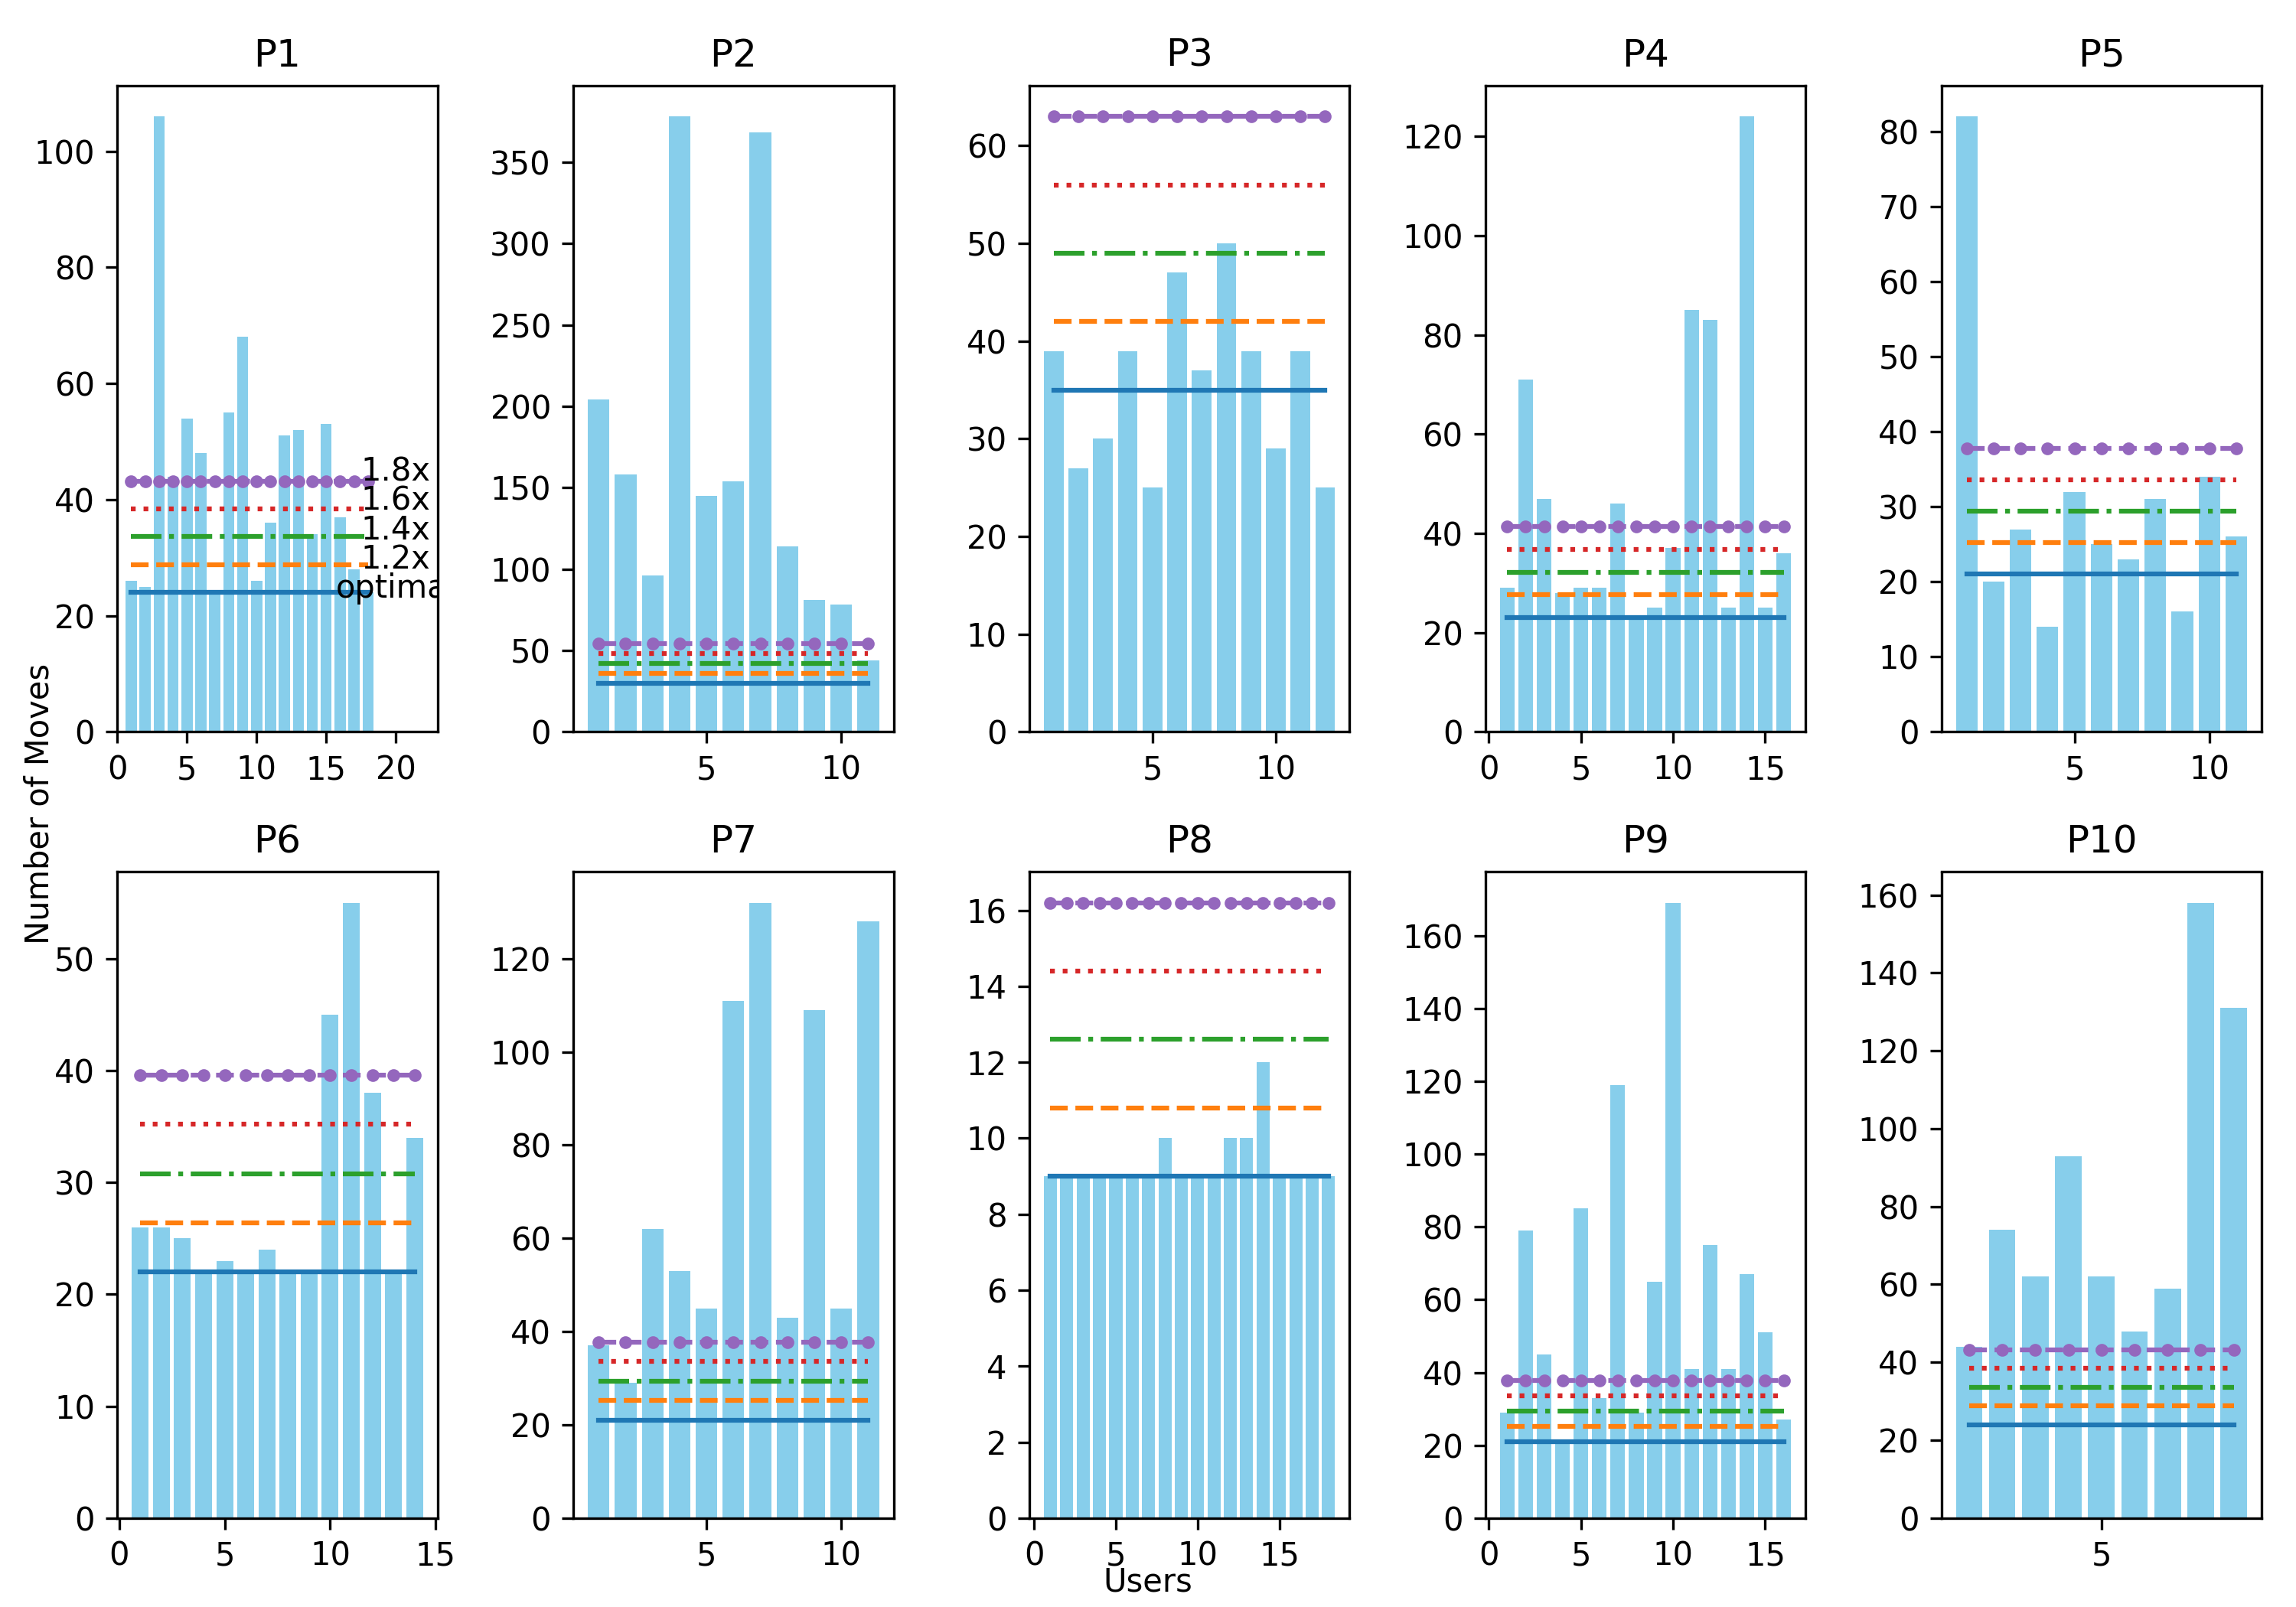
\includegraphics[width=\columnwidth]{img/difficulty.png}
  \caption{Number of moves in the users' solution compared to the optimal number of moves, and 1.2x, 1.4x, 1.6x, 1.8x the optimal number of moves for puzzles P1 through P10}
  \label{fig:difficuly}
\end{figure}

For each puzzle, we sorted users' solutions by the number of moves in the ascending order and split them into three groups (fast, medium, slow). We ensured that the three groups for each puzzle contained approximately equal number of users. Table \ref{tab:solvergroups} summarizes the findings. There were 46 users in the Fast group, 42 in the Medium and 48 in the Slow group. Mean refers to the mean number of moves in a solution produced by users who solved a specific puzzle. Forbidden moves refers to the number of times, the users who solved a specific puzzle moved the forbidden vehicle. Here, we consider the complete solution (i.e., moves from the initial state to the goal state).

\begin{table}[ht]
\begin{tabular}{|l|l|l|l|l|l|l|}
\hline
\multicolumn{1}{|c|}{\multirow{2}{*}{PID}} &
  \multicolumn{2}{c|}{Fast (46)} &
  \multicolumn{2}{c|}{Medium (42)} &
  \multicolumn{2}{c|}{Slow (48)} \\ \cline{2-7} 
\multicolumn{1}{|c|}{} &
  \multicolumn{1}{c|}{Mean} &
  \multicolumn{1}{c|}{\begin{tabular}[c]{@{}c@{}}Forbidden\\ Moves\end{tabular}} &
  \multicolumn{1}{c|}{Mean} &
  \multicolumn{1}{c|}{\begin{tabular}[c]{@{}c@{}}Forbidden\\ Moves\end{tabular}} &
  \multicolumn{1}{c|}{Mean} &
  \multicolumn{1}{c|}{\begin{tabular}[c]{@{}c@{}}Forbidden\\ Moves\end{tabular}} \\ \hline
P1  & 25.5 & 0  & 41.7  & 0  & 64.7  & 0  \\ 
P2  & 74.7 & 4  & 137.7 & 16 & 277   & 28 \\ 
P3  & 26.5 & 8  & 36.2  & 9  & 43.7  & 6  \\ 
P4  & 25.2 & 1  & 32    & 4  & 76    & 28 \\ 
P5  & 18.3 & 3  & 26    & 2  & 44.75 & 13 \\ 
P6  & 22   & 0  & 24.5  & 0  & 39.6  & 0  \\ 
P7  & 38.5 & 5  & 53.3  & 16 & 120   & 37 \\ 
P8  & 9    & 0  & 9     & 0  & 10    & 0  \\ 
P9  & 27.8 & 8  & 48.6  & 12 & 99    & 28 \\ 
P10 & 50.3 & 11 & 66    & 14 & 127.3 & 46 \\ \hline
\end{tabular}
\caption{Human solvers grouped by the mean number of moves and the corresponding forbidden moves}
\label{tab:solvergroups}
\end{table}

We can see that the longer the users' solutions are the more they will be moving the forbidden vehicle. Is this relationship statistically significant? We first perform the normality test between the two variables: number of moves and the number of times the forbidden car was moved. We used the Shapiro-Wilks test for the two distributions with $H_0:$ the distribution is normally distributed, and $H_A:$ the distribution is not normally distributed. Given $\alpha=0.05$, Shapiro-Wilks test gives that the p-value $<0.05$ for both forbidden vehicle moves and the number of moves. Thus we reject $H_0$ for both distributions.

To test the relationship between the number of moves and the forbidden vehicle moves, we define the null and alternative hypotheses as follows. Since we showed that there is evidence that the distributions are not normally distributed, we use the non-parametric test, Spearman's Rank Correlation to test the strength of relationship. Let $\rho_s$ be the Spearman's population correlation coefficient:
\begin{itemize}
\item $H_0: \rho_s=0$, there is no correlation between the two variables
\item $H_A: \rho_s\neq0$, there is a correlation between the two variables
\end{itemize}
Given $\alpha=0.05$, Spearman's rank correlation coefficient is $\rho_s=0.52$ and p-value $<0.05$. Thus we reject the null hypothesis.

We now describe the behavior features we extract from a partial solution.
\begin{description}
\item[\texttt{len}:] number of moves in the partial solution
\item[\texttt{len-opt}:] difference of the number of moves in the user's partial solution and the number of steps in the safe optimal solution produced by an automated planner
\item[\texttt{undos}:] number of 1-step undo in the user's partial solution
\item[\texttt{forbidden}:] number of times the forbidden vehicle is moved
\item[\texttt{first}:] number of moves until the forbidden vehicle was moved for the first time
\item[\texttt{prop}:] number of moves until the forbidden vehicle was moved for the first time divided by the number of moves in the safe, optimal solution
\item[\texttt{moved}:] number of vehicles moved in the partial solution
\end{description}

\subsection*{Learning Methods}
We ask three learning questions:
\begin{itemize}
\item Can we predict whether or not the user will move the forbidden car one step before it actually happens?
\item Can we predict whether or not the user will move the forbidden car two steps before it actually happens?
\item Can we predict whether or not the user will move the forbidden car there steps before it actually happens?
\end{itemize}

In order to answer these three questions, we first partition the data set into training (70\%) and test (30\%) sets. Each user solution is filtered to only include the moves until one step, two steps and three steps before the forbidden car was moved for the first time. We then filter the features to remove features that are obvious indicators of forbidden car movements, specifically first, prop and forbidden. We use the remaining features to train five classifiers to respond to each learning question with 10-fold cross validation. In this work, we explore a number of classifier learning methods: the decision tree, random forest, K-nearest neighbor, Logistic Regression and Naive Bayes. The classifiers are used in the supervised learning mode. We summarize the parameters used in each learning method below:
\begin{itemize}
\item \textit{Decision Tree:} We use the J48 classifier available on the WEKA platform \cite{hall09}. This classifier implements the C4.5 algorithm \cite{quinlan1993c45}. The decision tree classifier is tuned to user pruning confidence=0.25 and the minimum number of instance per leaf=2.
\item \textit{Random Forest:} This classifier is tuned to use bagging with 100 iterations and a base learner. These configuration parameters are available on the WEKA platform. 
\item \textit{k Nearest Neighbor:} We use this classifier with a Euclidean distance metric, considering the value $k=1$
\item \textit{Logistic Regression:} This classifier is tuned for ridge parameter $= 1.0E-8$.
\item \textit{Naive Bayes:} This classifier is tuned with the supervised discretization=True.
\end{itemize}

\subsection*{Results}
We then use each learned model on the test data set to predict the class for each user, i.e, whether the user be intervened or not given his partial solution. Table \ref{tab:accuracy} summarizes the precision, recall and F-measures for the three soft intervention models.
It can be seen that the Logistic Regression classifier performs best with high precision/recall compared to other classifiers when predicting soft intervention 1 or 2 steps early. The Logistic Regression classifier also predicts intervention 3 steps early with high recall albeit with slightly lower precision. As the prediction window expands, the precision of the decision tree classifier improves. However, the recall and F measures drop when predicting intervention 3 steps early. The Naive Bayes classifier reported the lowest precision compared to all other classifiers for all three intervention windows. It is interesting to note that the Random Forest classifier performs better than the Decision Tree when the intervention window is 1 and 3 steps. The accuracy drops for the Random Forest when the prediction window is 2.

\begin{table}[htb]
\begin{tabular}{|l|l|l|l|}
\hline
Q1 &
  \multicolumn{3}{l|}{\begin{tabular}[c]{@{}l@{}}Predict whether the user will be moving the forbidden car one\\ step before the move actually happens\end{tabular}} \\ \hline
\textbf{Classifier} &
  \textbf{Precision} &
  \textbf{Recall} &
  \textbf{F1} \\ \hline
Decision Tree       & 0.7  & 0.9  & 0.79 \\ 
Random Forest       & 0.76 & 0.9  & 0.83 \\ 
k Nearest Neighbor  & 0.89 & 0.76 & 0.82 \\
Logistic Regression & 0.91 & 0.95 & 0.93 \\ 
Naive Bayes         & 0.73 & 0.9  & 0.81 \\\hline
Q2 &
  \multicolumn{3}{l|}{\begin{tabular}[c]{@{}l@{}}Predict whether the user  will be moving the forbidden car two\\ steps before the move actually happens\end{tabular}} \\ \hline
Decision Tree       & 0.8  & 0.95 & 0.87 \\
Random Forest       & 0.75 & 0.86 & 0.8  \\ 
k Nearest Neighbor  & 0.86 & 0.86 & 0.86 \\ 
Logistic Regression & 0.87 & 1    & 0.93 \\
Naive Bayes         & 0.74 & 0.86 & 0.83 \\ \hline
Q3 &
  \multicolumn{3}{l|}{\begin{tabular}[c]{@{}l@{}}Predict whether the user  will be moving the forbidden car three\\ steps before the move actually happens\end{tabular}} \\ \hline
Decision Tree       & 0.89 & 0.81 & 0.85 \\ 
Random Forest       & 0.86 & 0.9  & 0.88 \\
k Nearest Neighbor  & 0.95 & 0.9  & 0.93 \\ 
Logistic Regression & 0.91 & 0.95 & 0.93 \\ 
Naive Bayes         & 0.68 & 0.9  & 0.78 \\ \hline
\end{tabular}
\caption{Precision, Recall and F-measure for the prediction accuracy for the three soft intervention learned models.}
\label{tab:accuracy}
\end{table}

\section*{Supporting Human Users with Soft Intervention}
We extend our soft intervention model to help human users complete cognitively engaging tasks by providing helpful hints. In the context of the Rush Hour puzzle solving task, a hint is a piece of information about the Rush Hour search problem. Hints are a special type of answer because they do not directly provide the complete solution to the problem (e.g., remaining moves to solve the Rush Hour puzzle). Our design of helpful hints allows the user to carefully probe the search space of the Rush Hour puzzle while avoiding the undesirable state. Hints are specially useful in situations where the human user wishes to retain some autonomy over the system he is interacting with (e.g., intelligent tutoring systems).
Formally, a hint is a function of the state space of the search problem. We represent the Rush Hour search problem as the planning task $\Pi_{agent}$ and the solution to which is a plan $\pi_{agent}$.
\begin{definition}
Given a partial user solution $\pi^\prime _{user}$, the initial state $I$, the user's goal $G_x$, and the undesirable state to avoid is $G_y$, we define the current state $s = \Delta (I,\pi^\prime _{user})$. Then, a hint is a function defined as: $\mathcal{H}(s,\lbrace G_x,G_y\rbrace) \rightarrow \Psi[\pi_{agent}]$, where $\Psi[\pi_{agent}]$ refers to some information about the solution plan $\pi_{agent}$.
\end{definition}
We conducted a human subject experiment to evaluate five hint types.
\begin{itemize}
\item Number of remaining moves, if $\Pi_{agent}$ is solved optimally, optimized for the number of moves.
\item Next move, if $\Pi_{agent}$ is solved optimally, optimized for the number of moves
\item The list of vehicles that must be moved to solve $\Pi_{agent}$
\item Restart game (i.e, restore $s$ back to $I$)
\item Ignore hint. Two successive choices of this option disables the hints.
\end{itemize}

For this study, we recruited 140 subjects from a graduate and undergraduate university student population. The participants were not compensated for their time. The sample comprised of college undergraduate and graduate students in Computer Science, Microbiology, Chemistry, Business majors. After obtaining informed consent, the participants were directed to the Web URL, which hosted the Rush Hour simulator software. In this study, we added three new functional features to the simulator, namely: an automated planner to probe the search space, a landmark computation component to support hint generation, and the soft intervention learned model.

Each participant was assigned to solve one Rush Hour puzzle randomly selected from a set of thirteen. We did not place any time restriction for the puzzle solving task. Participants were randomly assigned to two groups; one group was asked to watch a 44 second video tutorial on how the Rush Hour puzzle can be solved by avoiding the forbidden vehicle. This group was only allowed to start the puzzle after watching the video. The other group did not watch the video. Instead they were allowed to immediately start the puzzle. Additionally, all participants had the option to use an online tutorial (available on the simulator itself) on how to play the Rush Hour puzzle. Each of the thirteen puzzles contained one forbidden vehicle. Participants were informed that one of the vehicles on the game board is forbidden and the puzzle must be solved without moving the forbidden vehicle. In this phase, the simulator produced an alert message when the soft intervention learned model predicted that, based on the user's partial solution, the user will be moving the forbidden vehicle 1 move later. The alert message displayed the five hints (see Figure \ref{fig:help}) and the user is asked to select one. Based on the choice, a second alert message is shown, which contains the information $\Psi[\pi_{agent}]$. Once the puzzle solving task was completed, the participants were asked to complete a short demographic survey and rate the helpfulness of each hint type in avoiding the forbidden vehicle. Figure \ref{fig:phase2} illustrates the activity sequence of the experiment.

\begin{figure}[!htb]
  \centering
  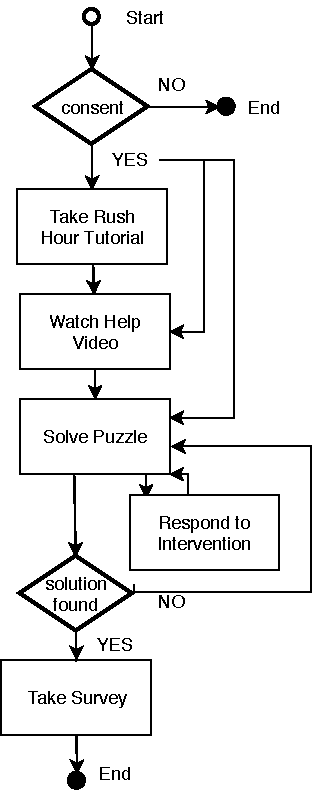
\includegraphics[height=0.6\columnwidth]{img/phase2.pdf}
  \caption{Activity sequence for evaluating hints during intervention for the Rush Hour human subject experiment}
  \label{fig:phase2}
\end{figure}

\subsection*{The Planning Component}
Two of the hints: number of remaining moves and next move, use the planning component. Our design of the planning component use the Fast Downward planner \cite{helmert2006} with the LM-cut heuristic (admissible) to find optimal plans, optimized for the number of moves. Given a partial user solution $\pi^\prime _{user}$, the initial state $I$, the user's goal $G_x$, and the undesirable state to avoid is $G_y$, we define the current state $s = \Delta (I,\pi^\prime _{user})$. Then, the planning component generates the planning task $\Pi_{agent} = \langle \mathcal{F}, \mathcal{A}, s, G \rangle$, where $\mathcal{F}$ is the propositions grounded with the objects $\mathcal{O}\setminus o_f$ where $o_f$ is the forbidden vehicle, $\mathcal{A}=A_d$ (i.e., actions that are not grounded with $o_f$), $s$ is the new initial state (i.e., state after executing the partial solution) and $G = G_x$ (i.e, target vehicle being at the exit).
The solution to $\Pi_{agent}$ is the plan $\pi_{agent}$, which is a sequence of actions $\lbrace a_1, a_2, \ldots, a_n\rbrace$, where $a_i \in \mathcal{A}$. Because we are using an admissible heuristic to find the plan, $\pi_{agent}$ is also the optimal plan to solve the puzzle from the current state $s$. When the user requests for the hint \textbf{number of remaining moves}, $\Psi[agent]=c(\pi_{agent})$, which refers to the cost of $\pi_{agent}$. Since we are assuming actions are of unit cost, this is equivalent to the number of actions in $\pi_{agent}$. This hint gives the user an indication of how many more moves the user needs to minimally make to solve the puzzle from the current state while avoiding the undesirable state. Similarly, when the user requests for the hint \textbf{next move}, $\Psi[agent]=a_1$, which is the first action in $\pi_{agent}$. This information tells the user the next action to execute if the user were to solve the puzzle with the minimum number of moves from the current state while avoiding the undesirable state.

The hint for the \textbf{list of vehicles that must be moved} requires us to find the landmarks for the planning task $\Pi_{agent}$. \textit{A landmark of a planning task are facts that must be true at some point during the execution of any solution plan} \cite{hoffman2004lm}. By this definition, the initial and the goal facts are trivially landmarks. We use the Ordered Landmark algorithm \shortcite{hoffman2004lm} to find landmarks in the planning task $\Pi_{agent}$. This algorithm uses a data structure called the Landmark Generation Graph (LGG) to find the landmarks and the greedy necessary orders between them. Nodes in LGG are the landmark propositions and the edges are the greedy-necessary orders. Starting from the goal (the first landmark candidates), the algorithm uses the back-chaining process to find the earliest actions that can be used to achieve each landmark. Here, early means a greedy approximation of reachability from the initial state. The landmark achievers are actions in $\mathcal{A}$. The landmark achievers are grounded with the objects that must be moved to solve the puzzle from the current state.

The two other hints \textbf{Restart} and \textbf{Ignore} are the last-resort kind of help. The restart game hint simply reverts the game state $s$ back to the initial state $I$ and allows the user to start from the beginning. In the experiment setup, we did not enforce any limits on the number of times a participant can restart a game. The ignore hint allows the user to continue the puzzle solving task. This does not modify the current game state. However, in the experiment setup we enforced a condition that if the participant selects the ignore option twice in a row, the intervention help system will permanently deactivate.

\subsection*{The Learning Component}
We use the Logistic Regression classifier learned from human solvers' solutions in the previous study to predict intervention in this experiment. Our learned models operate within three intervention intervals, where the user is intervened either one step before, two steps before or three steps before the forbidden vehicle is moved. For this experiment, we used the Logistic Regression classifier trained to intervene one step before the undesirable state. This classifier had the highest precision, recall and F measures compared to all other classifiers we experimented with.

Given a partial user solution $\pi^\prime _{user}$, and the initial state $I$, we define the current state $s = \Delta (I,\pi^\prime _{user})$. We then compute the feature values corresponding to the current game state ($s$) and also the feature values corresponding to the partial solution $\pi^\prime _{user}$. Then the feature vector combining both game state and partial solution features are provided as input to the classifier and a decision is obtained whether to intervene or not. If an intervention occurs the user is shown a set of hints. If not the user continues to solve the puzzle. This cycle continues for each new move the user makes unless the user instructs the system to stop intervention by choosing the Ignore Hint option.

%results
\subsection*{The Human Subject Experiment}
\subsubsection*{Experimental Design}
Our second human subject experiment evaluates how human solvers use the helpful hints during the Rush Hour puzzle solving task. As shown in Table \ref{tab:puzzles} (right), we created thirteen unique Rush Hour puzzles. We used ten puzzles (P1 through P10) from the previous study and added three new puzzles so that each puzzle type (A, B, C) had approximately the same number of puzzles. For this study, we recruited subjects from a graduate and undergraduate university student population. The participants were not compensated for their time. After obtaining informed consent, the participants were directed to the Web URL, which hosted the Rush Hour simulator software. In this experiment, the simulator software lets the user solve a puzzle but offers helpful hints upon recognizing the user may move the forbidden vehicle 1 step ahead into the future.

Before starting the puzzle solving task, the participants were randomly assigned to two groups. One group were shown a 44 second video of a Rush Hour puzzle solving task. The video showed a solution, which did not move the forbidden vehicle. Participants in this group were only allowed to continue on to the puzzle solving task after watching the video. Figure\ref{fig:video} illustrates the video screen. The other group did not see the video and was directed to start the puzzle solving task immediately. Each participant was assigned to solve one Rush Hour puzzle randomly selected from the set of thirteen. We did not place any time restriction for the puzzle solving task. All participants had the option to use an online tutorial (available on the simulator itself) on how to play the Rush Hour puzzle. All thirteen puzzles contained a forbidden vehicle. Participants were informed that one of the vehicles on the game board is forbidden and the puzzle must be solved without moving the forbidden vehicle. 

\begin{figure}[!htb]
  \centering
  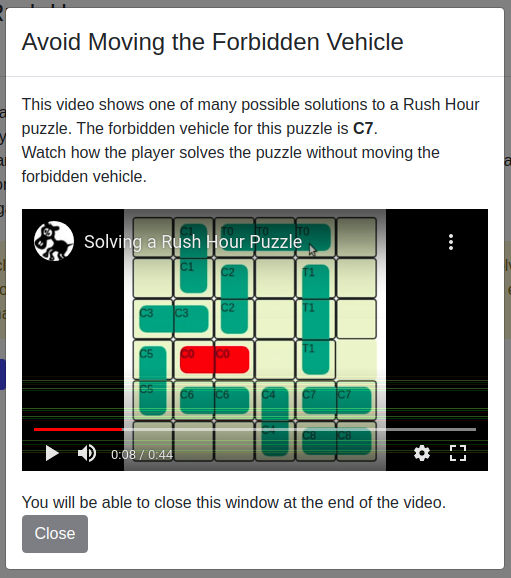
\includegraphics[width=0.6\columnwidth, keepaspectratio=true]{img/help.png}
  \caption{Help video screen}
  \label{fig:video}
\end{figure}

During the puzzle solving task when the decision to intervene is made, the participant sees pop-up message shown in Figure \ref{fig:help}, which offers four hints and the ignore option. Based on the choice the user makes, a response is displayed. In addition, if the user moves the forbidden vehicle the simulator displays an alert shown in Figure \ref{fig:badcar}. When this happens, the game engine automatically undoes the forbidden vehicle move. These functionalities are different from the previous experiment conditions where the participant did not get any visual cues during game play.
\begin{figure}[!htb]
  \centering
  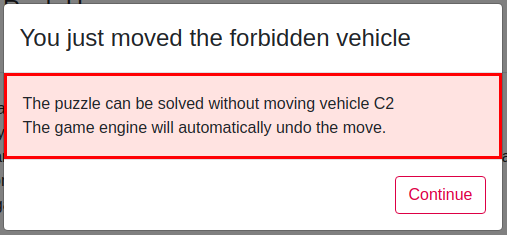
\includegraphics[width=0.5\columnwidth, keepaspectratio=true]{img/badcaralert.png}
  \caption{Forbidden vehicle move alert message}
  \label{fig:badcar}
\end{figure}
Once the puzzle solving task is completed, the participants are asked to complete a short survey to capture the demographics and also asks them to subjectively rate the helpfulness of each hint type on a 5-point Likert scale. 142 subjects participated the study. We removed records from seven participants from the analysis because they had quit the session mid-play, leaving 135 usable records. The sample comprised of college undergraduate and graduate students in Agriculture, Biology, Animal Sciences, Computer Science, Engineering, Horticulture, and Business majors. 131 of the 135 participants also completed the demographics survey.


RESULTS TBD




%%%%%%%%%%%%%%%%%%%%%%%%%%%%%%%%%%%%%%%%%%%%%%%%%%%%%%%%%%%%%%%%
\chapter{Planned Research}

We are interested in how automated planning and machine learning methods can be used to automatically recognize when a human user is about to do something they should not (e.g., click on a phishing email, move the forbidden vehicle). Let us first revisit the three major questions this research is trying to address introduced in Chapter 1.
\begin{itemize}
\item What are the salient characteristics for deciding when to intervene?
\begin{itemize}
\item when the user's goals \textbf{are known} (simulated in the Rush Hour domain)
\item when the user's goals \textbf{are not known} (simulated in the cyber-security domain)
\end{itemize}
\item How to help task continuation following intervention?
\item How to design tools to study intervention with human user participation?
\end{itemize}

Our intervention models are based on identifying pivotal actions in an observations of user actions that are critical to cause an undesirable state. This requires that we evaluate the
current state (i.e., state resulting from the observed action) based on how critical it is to
cause the undesirable state. In the two case studies we evaluate the criticality using two
different methods. For the cyber-security domain, we first model the domain as a STRIPS planning task and we identify salient features of the pivotal states by analyzing the plan space generated by the planning task. For the Rush Hour domain, we estimate the criticality of the current state using user behavior features extracted from the puzzle state.

Although we discuss two specific domains in this research, two of the three recognition algorithms we propose are domain-independent. This means that the salient characteristics that determine the decision to intervene are extracted from the planning problem representation and therefore can also be extended to be evaluated on benchmark planning domains. However, the two planning domains have unique characteristics in their representations and the assumptions we make for each case.

As illustrated in Figure~\ref{fig:breakdown} this research proposes three intervention algorithms. 
\begin{itemize}
\item Intervention by critical action recognition
\item Intervention by unhelpful plan prefix recognition
\item Intervention by user behavior classification.
\end{itemize}

\section*{Completed Tasks}
We plan to accomplish these three milestones following the tasks T1 through T8. Presently, we have completed tasks T1, T2, T4, T5, and T6. 

Task T7 is now in progress. The data collection for T7 is complete. We are now developing the learned models to recognize when the user needs help.

\begin{figure}[!htb]
  \centering
  \includegraphics[width=\columnwidth, keepaspectratio=true]{img/tasks.pdf}
  \caption{Research Task Breakdown}
  \label{fig:breakdown}
\end{figure}



%What are the differences between these two domains?
%Cyber-security experiment
%	Intervene by identifying critical actions
%Benchmarks
%	Intervene by identifying unhelpful plan prefix
%Rush Hour
%	Intervene by learning from user's behavior
	

\section*{Planned Work}
\textbf{T3: Intervention in Cyber-security Domain}\\
For the cyber-security domain we identify salient features of the critical state by analyzing the plan space of undesirable plans. Here, we assume that the user's goal is unknown. This is in line with the idea that it is difficult to anticipate a human user's goal, which may change from time to time. Therefore, unlike in the plan prefix recognition algorithm where we assumed the observer knows the user goal, we can not compare against a sample of helpful plans. Our idea is to model the cyber-security domain as a planning problem and use an existing automated planner to  sample the possible solutions (plans) that project possible undesirable outcomes and then trace back to actions critical to their occurrence.

We treat the undesirable plan (UP) achieving the undesirable goal state as the `ground truth' trace.

\textbf{T3: Experiment 1}\\
\textbf{Question}: How well did the proposed algorithm recognize critical actions in traces produced by human users?\\
\textbf{Method}:\\
Since activity logs captured during the experiment could not be properly controlled for extraneous and missing actions, we limit the assessment to accuracy of the cyber-security domain observations to the effect imposed by adjusting the weight of each decision metric. The weight assignments will systematically enable/disable the metrics that we use in the decision making process. When the algorithm identifies a critical action, it must (1) be an action that will appear in a ground truth plan and (2) it must not be an extraneous (noisy) action. Given these two conditions we can define the accuracy as the sum of (1) and (2). Then measure accuracy, by varying the metric weight assignments.\\
\textbf{Expectation} Identify which weight assignments provide best accuracy for recognizing critical actions in human user plans.

\textbf{T3: Experiment 2}\\
\textbf{Question}: What is the time cost of the proposed algorithm recognize critical actions in traces produced by human users?\\
\textbf{Method}:\\
Measure CPU time in seconds for the time period between the observation was submitted into the algorithm and critical action identification decision was produced.\\
\textbf{Expectation} Identify how long does it take for the algorithm to render its intervention decision. This allows us to evaluate whether or not the proposed algorithm could easily be integrated into an agent that mitigates cyber-security issues.
 
\textbf{T3: Experiment 3}\\
\textbf{Question}: Does the critical action recognition algorithm generalize to other planning domains?\\
\textbf{Method}:\\
We will select four benchmark planning domains (Blocks Words, IPC-Grid, Logistics and Navigator) from the International Planning competition planning problems. We will generate recognition problems for each planning domain for four undesirable states and corresponding plans using a diverse planner. The plans allows us to control for partial observability and noise in the observation traces given as input to the algorithm. We will consider partial observability ratios in the trace such that 25\%, 50\%, 75\%, 100\% from least observable to fully observable by removing actions in the trace.\\ We simulate extraneous actions in the trace by adding random actions that should not be in the solution plan into the trace such that 0\%, 50\%, 75\%, 100\%, from no extraneous actions to all extraneous actions.\\
\textbf{Expectation} A new test benchmark suite that can evaluate recognition algorithms with controlled levels of partial observability and extraneous actions.

\textbf{T3: Experiment 4}\\
\textbf{Question}: Does the critical action recognition algorithm avoid flagging noisy actions in the benchmark domains?\\
\textbf{Method}:\\
For observation traces in each class of noise levels, run the algorithm and record the count of times the algorithm did not flag a noisy action as the critical trigger action and compute the mean for that particular noise level. Repeat the experiment for varying metric weight assignments.
\\
\textbf{Expectation} Identify which decision metrics in the algorithm are sensitive to noise in the observation trace


\textbf{T3: Experiment 5}\\
\textbf{Question}: How the critical action recognition algorithm accuracy gets affected when there is partial observability in the benchmark domains?\\
\textbf{Method}:\\
For observation traces in each class of missing action levels, run the algorithm and record the count of times the algorithm accurately flagged a critical action that is also in a predefined ground-truth plan and compute the mean accuracy for that particular missing level. Repeat the experiment for varying metric weight assignments.
\\
\textbf{Expectation} Identify which decision metrics in the algorithm are sensitive to missing actions in the observation trace.

\textbf{T3: Experiment 6}\\
\textbf{Question}: What is the time cost of the proposed algorithm recognize critical actions in benchmark planning domains?\\
\textbf{Method}:\\
Measure CPU time in seconds for the time period between the observation was submitted into the algorithm and critical action identification decision was produced, for each observation trace in noise levels and missing action levels\\
\textbf{Expectation} Identify the effect of time for varying levels of noise and missing actions.
 






\textbf{T7: Human Behavior Features and Classifiers}

We are using the properties derived from the game state (positions of objects on the board) and the properties of the users' partial solution that has been observed up to now to extract features that correspond to the user's game play behavior. We plan to derive classifiers to answer three learning questions:

\begin{itemize}
\item Can we predict whether or not the user will move the forbidden car one step before it actually happens?
\item Can we predict whether or not the user will move the forbidden car two steps before it actually happens?
\item Can we predict whether or not the user will move the forbidden car there steps before it actually happens?
\end{itemize}

We will be using decision trees, logistic regression, k-nearest neighbor, random forests and Naive Bayes classifiers to evaluate how each classifier performs in recognizing intervention at the three different time steps.

\textbf{T7: Experiment 1}\\
\textbf{Question}: What classification models produce the best learned model for the user behavior classification?\\
\textbf{Method}:\\
Separate the data set collected from the Phase 1 experiment to 70\% training 30\% for testing. Run the selected classifiers on the training data with cross validation and generate the learned models. Run the learned models on the testing data set and calculate Precision, Recall and F-measures for the classifiers.

Repeat for the three learning questions.
\\
\textbf{Expectation} Identify which classification algorithms will accurately predict user behavior for the three learning questions.

\textbf{T8: Intervention with Helpful Hints}\\
Task T8 requires a few extensions to be added to the web simulator: a planner, the learned classifier and a hint generator. We will only integrate the top performing classifier into the web simulator. The implementations are now in progress.

We will conduct a human subject study that evaluates the effect of five helpful hints when human users solve Rush Hour puzzles. In the context of the Rush Hour puzzle solving task, a hint is a piece of information about the Rush Hour search problem. We designed helpful hints such that it allows the user to carefully probe the search space of the Rush Hour search problem, while avoiding the undesirable state.

\textbf{T8: Experiment 1}\\
\textbf{Questions}: \\
What were the most frequently used hints?\\
What is the effect on puzzle solution length on seeing hints?
\\
Did the hints help the user move closer to the optimal solution?\\
What is the effect on the number of times the forbidden vehicle was moved between the users who saw the hints and the users who did not?\\
\textbf{Expectation} Identify which hints the users found to be helpful.

I summarize the work that will be completed between December 2020 to July 2021 in Table~\ref{tab:planned}.
\begin{table}[]
\resizebox{\textwidth}{!}{%
\begin{tabular}{|l|l|l|}
\hline
\multicolumn{1}{|c|}{Timeline} &
  \multicolumn{1}{c|}{Task} &
  \multicolumn{1}{c|}{Notes} \\ \hline
Dec 2020 &
  T7/T8 &
  \begin{tabular}[c]{@{}l@{}}T7: Produce learned models from the data from Rush Hour experiment phase 1\\ T8: Finish coding for phase 2 extensions\end{tabular} \\ \hline
Jan 2021 &
  \begin{tabular}[c]{@{}l@{}}T3 \\ T8\end{tabular} &
  \begin{tabular}[c]{@{}l@{}}T3: Create benchmark planning problems test suite\\ T8: Recruit subjects, Testing and web application deployment\end{tabular} \\ \hline
Feb 2021 &
  \begin{tabular}[c]{@{}l@{}}T3\\ T8\end{tabular} &
  \begin{tabular}[c]{@{}l@{}}T3: Critical action recognition algorithm implementation\\ T3: Examine factors that affect the performance of the critical trigger recognition algorithm\\ Dependent variables: recognition accuracy, CPU time\\ Independent variables: objective weights, noise ratio, partial observability\\ T8: Collect data, journal article draft\end{tabular}  \\ \hline
Mar 2021 &
  T3 &   \begin{tabular}[c]{@{}l@{}}T8: Finish data collection (estimation $\approx$ 130 participants), result analysis, journal article\\ T3: Research article\end{tabular}
   \\ \hline
Apr 2021 &
  Dissertation Writing &
   \\ \hline
May 2021 &
  Dissertation Writing &
   \\ \hline
Jun 2021 &
  Revise Thesis &
   \\ \hline
Jul 2021 &
  Final Defense &
   \\ \hline
\end{tabular}%
}
\caption{Planned research between December 2020 to July 2021}
\label{tab:planned}
\end{table}
	
%one way would be to frame the user's task as a planning problem.
%that allows us to exploit the structure of the problem to extract features.
%thn the other way is to learn from user behavior.








































%%%%%%%%%%%%%%%%%%%%%%%%%%%%%%%%%%%%%%%%%%%%%%%%%%%%%%%%%%%%%%%%%%%
%  Appendices
%
%%%%%%%%%%%%%%%%%%%%%%%%%%%%%%%%%%%%%%%%%%%%%%%%%%%%%%%%%%%%%%%%%%%
\backmatter % starts unnumbered supplementary material
\appendix
\chapter{Cyber-security Experiment Materials: Pre-Study Survey}
\label{apx:cypre}
Dear Participant,\\
Thank you for participating in our user computer usage study. Please complete the following questionnaire as accurately as possible before completing the experiment tasks. The purpose of this questionnaire is to gather information about your computer usage patterns. The information you provide will be kept anonymous.\\
Please answer ALL questions.

\begin{enumerate}[topsep=-4em]
\item State your age in years
\begin{itemize}[topsep=-6em, label={o}]
\itemsep-1em 
\item 20 -- 25
\item 26 -- 30
\item 31 -- 35
\item 36 -- 40
\item 41 and above
\item I do not want to give that information
\end{itemize}
\item State your gender
\begin{itemize}[topsep=-6em, label={o}]
\itemsep-1em 
\item Male
\item Female
\item I do not want to give that information
\end{itemize}
\item State your education level
\begin{itemize}[topsep=-6em, label={o}]
\itemsep-1em 
\item Not currently in college - no bachelors or associates degree completed
\item Currently in college and working towards an associates degree
\item Currently in college and working towards a bachelors degree
\item Not currently in college - have completed bachelors degree within the last 5 years
\item Currently in college and working towards a graduate degree
\item Not currently in college - have a completed graduate degree
\item Other \rule{4cm}{0.4pt}
\item I do not want to give that information
\end{itemize}
\item How long have you been using computers?
\begin{itemize}[topsep=-6em, label={o}]
\itemsep-1em 
\item 1 -- 2 years
\item 3 -- 4 years
\item 5 -- 6 years
\item more than 6 years
\end{itemize}
\item How many hours per day do you use the computer?
\begin{itemize}[topsep=-6em, label={o}]
\itemsep-1em 
\item less than 2 hours
\item 2 -- 5 hours
\item 5 -- 8 hours
\item more than 8 hours
\end{itemize}
\item Which of the following computing devices do you own? (Select all that apply)
\begin{itemize}[topsep=-6em, label={o}]
\itemsep-1em 
\item Desktop PC
\item Laptop
\item Smart Phone
\item Tablet PC
\item E-reader
\item Other \rule{4cm}{0.4pt}
\end{itemize}
\item What software applications do you use regularly? (Select all that apply)
\begin{itemize}[topsep=-6em, label={o}]
\itemsep-1em 
\item Web browser (Internet Explorer, Firefox, Chrome)
\item Office application suite (Word processors, spreadsheets etc.)
\item Media players (windows media player, QuickTime, VLC media player etc.)
\item Adobe Acrobat Reader (for PDF files)
\item Computer games
\item Design and image processing applications (Adobe Photoshop, Flash, GIMP etc.)
\item Software development tools (Eclipse, Netbeans, IntelliJ IDEA)
\item Other \rule{4cm}{0.4pt}
\end{itemize}
\item For what purposes do you often use the computer? (Select all that apply)
\begin{itemize}[topsep=-6em, label={o}]
\itemsep-1em 
\item work/business
\item Education
\item Gathering information from the Internet (online news, weather, sports etc.)
\item Communicating with others (instant messaging, email, Facebook, Twitter etc)
\item Preparing documents, spreadsheets, presentations
\item Playing computer games
\item Financial activities (e.g. banking, online shopping, budgeting etc.)
\item Programming and other software design and development tasks
\item Other \rule{4cm}{0.4pt}
\end{itemize}
\item Which of the following tasks related to computer usage do you find most challenging? (Select all that apply)
\begin{itemize}[topsep=-6em, label={o}]
\itemsep-1em 
\item Finding application software that matches my requirements
\item Installing, configuring and getting a software application ready to be used
\item Finding and using help manuals
\item Identifying actions that may harm the computer
\item Taking steps to ensure the safety of the computer
\item Other \rule{4cm}{0.4pt}
\end{itemize}
\item Have you had any formal training to use the computer?
\begin{itemize}[topsep=-6em, label={o}]
\itemsep-1em 
\item I have taken computer programming courses (in college/university, online)
\item I have taken courses in using computer applications (in college/university, online)
\item I have followed online tutorials to learn how to use the computer
\item I have taken part in face-to-face seminars/tutorial classes on using the computer
\item Other \rule{4cm}{0.4pt}
\end{itemize}
\item Where do you go when you need help in how to use the computer? (Select all that apply)
\begin{itemize}[topsep=-6em, label={o}]
\itemsep-1em 
\item Internet
\item Relatives
\item Friends
\item Local stores (e.g., Apple Genius Bar)
\item Other \rule{4cm}{0.4pt}
\end{itemize}
\item Have you installed any anti-virus software in your personal computer?
\begin{itemize}[topsep=-6em, label={o}]
\itemsep-1em 
\item Yes
\item No
\end{itemize}
\item Which of the following commonly used software have you installed in your personal computer? (Select all that apply)
\begin{itemize}[topsep=-6em, label={o}]
\itemsep-1em 
\item Google Chrome
\item Mozilla Firefox
\item Microsoft Office Package (Microsoft Word, Microsoft Excel, PowerPoint etc.)
\item Opensource Office Package (LibreOffice, OpenOffice)
\item Apple QuickTime media player
\item VLC Media Player
\item Adobe Flash Player
\item Adobe Acrobat Reader
\item Skype
\item Third-party email clients (Thunderbird, Eudora, Outlook Express)
\item Other \rule{4cm}{0.4pt}
\end{itemize}
\end{enumerate}


\chapter{Cyber-security Experiment Materials: Post-Study Survey}
\label{apx:cypost}
\begin{enumerate}[noitemsep]
\item What was the full name you used for this study?
\item How difficult was it for you complete the Install and configure Antivirus software task?\\
Very Hard \hspace{1cm} Hard \hspace{1cm} Neither easy nor hard \hspace{1cm} Easy \hspace{1cm} Very easy 
\item I feel confident in my ability to configure and use an antivirus software.
\par Strongly Disagree \hspace{1cm} Disagree\hspace{1cm}Neutral\hspace{1cm} Agree\hspace{1cm} Strongly agree
\item I feel confident in my ability to select an antivirus software that matches my security requirements.
\par Strongly Disagree \hspace{1cm} Disagree\hspace{1cm}Neutral\hspace{1cm} Agree\hspace{1cm} Strongly agree
\item I feel confident in my ability to identify legitimate antivirus software.
\par Strongly Disagree \hspace{1cm} Disagree\hspace{1cm}Neutral\hspace{1cm} Agree\hspace{1cm} Strongly agree
\item I feel confident in my ability to identify and remove suspicious files on my computer using an antivirus software.
\par Strongly Disagree \hspace{1cm} Disagree\hspace{1cm}Neutral\hspace{1cm} Agree\hspace{1cm} Strongly agree
\item I feel confident in my ability to identify and remove suspicious files on my computer using an antivirus software without help.
\par Strongly Disagree \hspace{1cm} Disagree\hspace{1cm}Neutral\hspace{1cm} Agree\hspace{1cm} Strongly agree
\item Before choosing a source to download software, I first check if it is hosted by a trustworthy provider as it may expose me to a security threat.
\par Strongly Disagree \hspace{1cm} Disagree\hspace{1cm}Neutral\hspace{1cm} Agree\hspace{1cm} Strongly agree
\item I choose an antivirus software, which allows me to customize its features to match my security requirements.
\par Strongly Disagree \hspace{1cm} Disagree\hspace{1cm}Neutral\hspace{1cm} Agree\hspace{1cm} Strongly agree
\item I always use an antivirus software, configured to my preferred settings in my computer system.
\par Strongly Disagree \hspace{1cm} Disagree\hspace{1cm}Neutral\hspace{1cm} Agree\hspace{1cm} Strongly agree
\item Using an antivirus software to identify and remove suspicious files in my computer is important to me.
\par Strongly Disagree \hspace{1cm} Disagree\hspace{1cm}Neutral\hspace{1cm} Agree\hspace{1cm} Strongly agree
\item How difficult was it for you complete the Respond to direct messages from twitter account task?
\par Very Hard \hspace{1cm} Hard \hspace{1cm} Neither easy nor hard \hspace{1cm} Easy \hspace{1cm} Very easy
\item I feel confident in my ability to use the direct messaging feature in Twitter.
\par Strongly Disagree \hspace{1cm} Disagree\hspace{1cm}Neutral\hspace{1cm} Agree\hspace{1cm} Strongly agree
\item I feel confident in my ability to identify suspicious messages on Twitter.
\par Strongly Disagree \hspace{1cm} Disagree\hspace{1cm}Neutral\hspace{1cm} Agree\hspace{1cm} Strongly agree
\item I feel confident in my ability to identify suspicious messages on Twitter without help.
\par Strongly Disagree \hspace{1cm} Disagree\hspace{1cm}Neutral\hspace{1cm} Agree\hspace{1cm} Strongly agree
\item I feel confident in my ability to identify suspicious messages on Twitter even if it is the first time I had seen one.
\par Strongly Disagree \hspace{1cm} Disagree\hspace{1cm}Neutral\hspace{1cm} Agree\hspace{1cm} Strongly agree
\item Before following a link on Twitter, I first check if it was sent by an unknown sender or contains suspicious information.
\par Strongly Disagree \hspace{1cm} Disagree\hspace{1cm}Neutral\hspace{1cm} Agree\hspace{1cm} Strongly agree
\item I practice caution when I follow links sent to me on messages on Twitter as they may expose me to a security threat.
\par Strongly Disagree \hspace{1cm} Disagree\hspace{1cm}Neutral\hspace{1cm} Agree\hspace{1cm} Strongly agree
\item I do not follow links sent to me on Twitter messages, if the content looks suspicious.
\par Strongly Disagree \hspace{1cm} Disagree\hspace{1cm}Neutral\hspace{1cm} Agree\hspace{1cm} Strongly agree
\item When I see a message warning me about the security of a web site (e.g., expired certificate, http:// instead of https://) I am about to visit, I do not visit that web site.
\par Strongly Disagree \hspace{1cm} Disagree\hspace{1cm}Neutral\hspace{1cm} Agree\hspace{1cm} Strongly agree
\item I practice caution when responding to email from senders I am not familiar with.
\par Strongly Disagree \hspace{1cm} Disagree\hspace{1cm}Neutral\hspace{1cm} Agree\hspace{1cm} Strongly agree
\item I practice caution downloading attachments in emails from senders I am not familiar with.
\par Strongly Disagree \hspace{1cm} Disagree\hspace{1cm}Neutral\hspace{1cm} Agree\hspace{1cm} Strongly agree
\item When prompted to change default passwords I always change the password.
\par Strongly Disagree \hspace{1cm} Disagree\hspace{1cm}Neutral\hspace{1cm} Agree\hspace{1cm} Strongly agree
\item When I am changing passwords, I am confident in my ability to choose a strong password.
\par Strongly Disagree \hspace{1cm} Disagree\hspace{1cm}Neutral\hspace{1cm} Agree\hspace{1cm} Strongly agree
\item Are you capable of recognizing secure web pages from non-secure web pages?
\par Yes \hspace{1cm} No \hspace{1cm} I do not know
\item Was Twitter.com page you saw during the experiment a secure web page?
\par Yes \hspace{1cm} No \hspace{1cm} I do not know
\item When you are asked to submit private information to websites, are you concerned about the safety of information you give?
\par Yes \hspace{1cm} No \hspace{1cm} I do not know
\item  When you submit private information (passwords, email addresses) to websites, do you verify that the site is secure and your information is safe?
\par Yes \hspace{1cm} No \hspace{1cm} I do not know
\item During the experiment did you download the antivirus software from a secure web page?
\par Yes \hspace{1cm} No \hspace{1cm} I do not know
\item The descriptions given for two anti-virus programs (Security Shield and PCDoctor) were helpful in choosing what software to install.
\par Strongly Disagree \hspace{1cm} Disagree\hspace{1cm}Neutral\hspace{1cm} Agree\hspace{1cm} Strongly agree
\item How do you recognize a legitimate web page hosted by a trusted party from a illegitimate,
unsafe website? (Select all that apply)
\begin{itemize}[topsep=-6em, label={o}]
\itemsep-1em 
\item professional appearance (e.g, less flashy, formal writing etc.)
\item contact information (email, address, phone numbers) specified on the website
\item URL starting with https:\verb|//|
\item Content, and photos on the website look original and related to the host's products
\item Not displaying advertisements that belong to third parties
\item website is well known and popular
\item I do not know
\end{itemize}
\item How do you recognize harmful email (spam/phishing)? (Select all that apply)
\begin{itemize}[topsep=-6em, label={o}]
\itemsep-1em 
\item Email address is from a unrecognizable/unheard of domain and not relevant to the person or company represented in the email
\item contact information (email, address, phone numbers) specified on the website
\item Links on the email are not legitimate and not relevant to the person or company represented in the email
\item Incorrect grammar/spelling
\item Email greeting is not personalized (e.g., Dear Customer instead of Dear (Your Name) )
\item Email message contains attachments that seem irrelevant to email message
\item Email messages with threats (e.g., discontinuing a service if not responded, changing passwords and other private information without your acknowledgment etc.)
\item I do not know
\end{itemize}
\item  When installing a software do you usually read the end user license agreement?
\par Yes \hspace{1cm} No
\item If you answered NO, why did you decide not to read the license agreement? (Select the choice that seems MOST important)
\begin{itemize}[topsep=-6em, label={o}]
\itemsep-1em 
\item It is too long to read
\item It is worded in technical terms I do not understand
\item I do not ever read license agreements and no harm has happened to me
\item I have no choice but to click on accept, if I want to use the software
\item I do not think information on the license agreement is relevant to me
\end{itemize}
\item  Did you read the end user license agreement when downloading the anti-virus software during the experiment task?
\par Yes \hspace{1cm} No
\end{enumerate}

\chapter{Rush Hour Experiment Materials: Intervention Design Post-Survey}
\label{apx:rushpre}
Dear Participant,\\
Thank you for participating in our study. Please complete the following questionnaire as accurately as possible. The purpose of this questionnaire is to gather information about your interests in logic puzzle solving (e.g., Rush Hour, Sudoku, sliding puzzles). The information you provide will be kept anonymous. \\
Please answer ALL questions.

\begin{enumerate}[topsep=-4em]
\item State your age in years
\begin{itemize}[topsep=-6em, label={o}]
\itemsep-1em 
\item less than 20
\item 20 -- 25
\item 26 -- 30
\item 31 -- 35
\item 36 -- 40
\item 41 and above
\item I do not want to give that information
\end{itemize}
\item State your gender
\begin{itemize}[topsep=-6em, label={o}]
\itemsep-1em 
\item Male
\item Female
\item I do not want to give that information
\end{itemize}
\item Do you like solving logic puzzles in general (e.g., Sudoku, Sliding block puzzles)?
\par Strongly Disagree \hspace{1cm} Disagree\hspace{1cm}Neutral\hspace{1cm} Agree\hspace{1cm} Strongly agree
\item Did you like the Rush Hour puzzle solving task?
\par Strongly Disagree \hspace{1cm} Disagree\hspace{1cm}Neutral\hspace{1cm} Agree\hspace{1cm} Strongly agree
\item How many hours per day do you use the computer?
\begin{itemize}[topsep=-6em, label={o}]
\itemsep-1em 
\item less than 2 hours
\item 2 -- 5 hours
\item 5 -- 8 hours
\item more than 8 hours
\end{itemize}
\item What about solving logic puzzles that interest you the most? (Select all that apply)
\begin{itemize}[topsep=-6em, label={o}]
\itemsep-1em 
\item Fun and relaxing
\item Sharpens my critical thinking skills
\item Challenge my friends and family to beat my time/score
\item Other \rule{4cm}{0.4pt}
\end{itemize}
\item How often do you solve logic puzzles?
\begin{itemize}[topsep=-6em, label={o}]
\itemsep-1em 
\item More than once a day
\item Once a day
\item Once every two to three days
\item Once a week
\item Once every two to three weeks
\item Once a month
\item Other \rule{4cm}{0.4pt}
\end{itemize}
\item If the puzzle you are solving appear to be difficult, what do you most often do?
\begin{itemize}[topsep=-6em, label={o}]
\itemsep-1em 
\item Give up
\item Keep trying until I solve it
\item Ask for help (help guides, online forums etc.)
\item Other \rule{4cm}{0.4pt}
\end{itemize}
\item Imagine you are solving an all new puzzle that you have not seen before. If you were to get stuck while solving the puzzle, which of these options would you most like to be available?
\begin{itemize}[topsep=-6em, label={o}]
\itemsep-1em 
\item A suggestion/tip to help me get past the problem I am in now
\item A timely warning that lets me know my current strategy is faulty
\item A timely warning plus an explanation on how to avoid similar problems in the future
\item I do not want outside help. I want to solve a puzzle on my own
\item Other \rule{4cm}{0.4pt}
\end{itemize}
\item  What do you play logic puzzles on? (Select all that apply)
\begin{itemize}[topsep=-6em, label={o}]
\itemsep-1em 
\item Mobile
\item Gaming consoles (e.g., XBox)
\item Personal computer/laptop
\item Puzzle books, magazines, news papers
\item Other \rule{4cm}{0.4pt}
\end{itemize}
\end{enumerate}


\chapter{Rush Hour Experiment Materials: Evaluating Intervention Hints Post-Study Survey}
\label{apx:rushpost}
Dear Participant,\\
Thank you for participating in our study. Please complete the following questionnaire as accurately as possible. The purpose of this questionnaire is to gather information about your general impression on helpful hints that were produced during the Rush Hour puzzle solving task. The information you provide will be kept anonymous. \\
Please answer ALL questions.

\begin{enumerate}[topsep=-4em]
\item State your age in years
\begin{itemize}[topsep=-6em, label={o}]
\itemsep-1em 
\item less than 20
\item 20 -- 25
\item 26 -- 30
\item 31 -- 35
\item 36 -- 40
\item 41 and above
\item I do not want to give that information
\end{itemize}
\item What is your education background?
\begin{itemize}[topsep=-6em, label={o}]
\itemsep-1em 
\item Arts/Humanities
\item Business
\item Computer Science
\item Engineering
\item Other \rule{4cm}{0.4pt}
\end{itemize}
\item Have you solved a Rush Hour puzzle before?
\begin{itemize}[topsep=-6em, label={o}]
\itemsep-1em 
\item Yes
\item No
\end{itemize}
\item Did you see hint notifications during the puzzle solving task?
\begin{itemize}[topsep=-6em, label={o}]
\itemsep-1em 
\item Yes
\item No
\end{itemize}
\item The hints helped me avoid moving the forbidden vehicle while solving the puzzle BEFORE I knew what the forbidden vehicle was.
\par Strongly Disagree \hspace{1cm} Disagree\hspace{1cm}Neutral\hspace{1cm} Agree\hspace{1cm} Strongly agree
\item Rate the four hints based on how helpful they were for you to avoid moving the forbidden vehicle
\begin{itemize}[topsep=-6em, label={o}]
\itemsep-1em 
\item Hint 1: See the minimum remaining number of moves
\par (low) \hspace{0.5cm}1 \hspace{1cm} 2\hspace{1cm}3\hspace{1cm} 4\hspace{1cm} 5 \hspace{0.5cm} (high)
\item Hint 2: See the next best move 
\par (low) \hspace{0.5cm}1 \hspace{1cm} 2\hspace{1cm}3\hspace{1cm} 4\hspace{1cm} 5 \hspace{0.5cm} (high)
\item Hint 3: See the vehicles that must be moved
\par (low) \hspace{0.5cm}1 \hspace{1cm} 2\hspace{1cm}3\hspace{1cm} 4\hspace{1cm} 5 \hspace{0.5cm} (high)
\item Hint 4: Restart puzzle
\par (low) \hspace{0.5cm}1 \hspace{1cm} 2\hspace{1cm}3\hspace{1cm} 4\hspace{1cm} 5 \hspace{0.5cm} (high)
\end{itemize}

\end{enumerate}
%%%%%%%%%%%%%%%%%%%%%%%%%%%%%%%%%%%%%%%%%%%%%%%%%%%%%%%%%%%%%%%%
% Bibliography
%%%%%%%%%%%%%%%%%%%%%%%%%%%%%%%%%%%%%%%%%%%%%%%%%%%%%%%%%%%%%%%%
% unsorted BibTeX style
% check here for more:  https://www.sharelatex.com/learn/Bibtex_bibliography_styles
\newpage
\bibliographystyle{apacite} % apa style bibliography
%\bibliographystyle{aaai} % must have aaai17 added in preamble
\bibliography{refsicaps19.bib}
%%%%%%%%%%%%%%%%%%%%%%%%%%%%%%%%%%%%%%%%%%%%%%%%%%%%%%%%%%%%%%%%
\end{document}
